We now move on to a problem involving three-dimensional stress states. Consider a infinite medium in directions $\vect{e}_2$ and $\vect{e}_3$ and of length $L=6\:m$ in direction $\vect{e}_1$. Riemann-type initial conditions similar to those treated above are assumed to yield the following infinitesimal strain and Cauchy stress tensors:
\begin{align*}
  & \tens{\eps}= \eps \vect{e}_1 \otimes\vect{e}_1 \\
  & \tens{\sigma}=\sigma_L \vect{e}_1 \otimes \vect{e}_1 + \sigma_T \(\vect{e}_2 \otimes \vect{e}_2+\vect{e}_3 \otimes \vect{e}_3\) 
\end{align*}
which correspond to the plane wave case. In that configuration, a relation depending on the constitutive model considered exists between longitudinal and transverse stress components $\sigma_L$ and $\sigma_T$. As a consequence, a one-dimensional hyperbolic system is solved for $\sigma_L=\sigma$, and the transverse component is computed subsequently. In this section, the behavior of the DGMPM on relaxation systems (see section \ref{sec:general-formulation}) is looked at by considering a solid made of an elastic-viscoplastic material following Perzyna, or Sokolowskii-Malvern, model with linear kinematic hardening \cite{Perzyna}. In the asymptotic limit $\tau = (\eta/\sigma^y)^n\rightarrow 0$, where $\tau$ is the relaxation time, the computed elastic-viscoplastic solution should tend to the elastoplastic one derived in \cite{Thomas_EP}, the latter being studied afterwards. 
% \begin{table}[h!]
%   \centering
%     \begin{tabular}{l|lN}
    \hline
    $E=2\times 10^{11}\:Pa$ & $\sigma^y=1 \times 10^8 Pa$ & \\ [3pt]
    $\nu=0.3$ & $C=10^{8} Pa$  &\\[3pt]
    $\rho_0 = 7800 \: kg.m^{-3}$ & &\\[3pt]
    \hline
  \end{tabular}

%%% Local Variables:
%%% mode: latex
%%% TeX-master: "../manuscript"
%%% End:

%   \caption{Material parameters. The viscosity is expressed as a function of the relaxation time $\tau$.}
%   \label{tab:material}
% \end{table}
The writing of the viscosity as a function of the relaxation parameter in table \ref{tab:material} enables the tuning of the stiffness of the hyperbolic system by setting different values of $\tau$.
%Table \ref{tab:material} lists the values of material parameters considered. In particular, the viscosity $\eta$ is a function of the relaxation time that is used to tune the stiffness of the problem.  
The solid is initially in a free stress state and the initial velocity is set so that plastic flow occurs:
\begin{equation*}
  v_0=2\frac{Y_H}{\rho c_L}
\end{equation*}
where $Y_H=(\lambda+2\mu)/2\mu$ denotes the Hugoniot elastic limit, $c_L=\sqrt{(\lambda+2\mu)/\rho}$ is the elastic pressure wave speed, and $(\lambda,\mu)$ Lam\'e's parameters. Both ends of the medium are traction free so that rightward and leftward compression elastic waves reflect as unloading waves that interact with the incident plastic ones \cite{Thomas_EVP}.

\subsubsection{Elastoviscoplasticity}
The elastic-viscoplastic problem is solved with the MPM using both USL and USF formulations, the DGMPM-Euler with Godunov splitting, and the DGMPM-RK2 coupled to Strang splitting. The latter formulation is however not used for the stiff setting since this fractional method is known to not be well-suited in that case \cite{Thomas_EVP,Leveque_stiff}. The ODE systems resulting from fractional approaches are discretized with an implicit backward Euler scheme for Godunov and a backward differentiation formula of order 3 for Strang splitting. The viscoplastic flow rule is then integrated explicitly at the end of the time step to update viscoplastic strains. On the other hand, constitutive equations are integrated with a radial return algorithm \cite{Simo} within the MPM. First, the relaxation system is considered in a non-stiff setting characterized by a relaxation time bigger than the time step governed by the convection part, that is $\tau=50\Delta t$. Figure \ref{fig:nonstiff_elastoviscoplastic_RP} shows a comparison of numerical stress and plastic strain with the exact solutions of the elastoplastic limit.
%Pas de RK2 godunov car le RK2 n'a une influence que sur la partie convective qui est équivalent au 1ppc Euler.
\begin{figure}[h!]
  \centering
  {\phantomsubcaption \label{subfig:evp_nonstiff1}}
  {\phantomsubcaption \label{subfig:evp_nonstiff2}}
  {\phantomsubcaption \label{subfig:evp_nonstiff3}}
  {\begin{tikzpicture}[scale=.9]
\begin{groupplot}[group style={group size=3 by 2,
ylabels at=edge left, yticklabels at=edge left,horizontal sep=2.ex,
vertical sep=4ex,xticklabels at=edge bottom,xlabels at=edge bottom},
ymajorgrids=true,xmajorgrids=true,enlargelimits=0,xmin=0.,xmax=6.,xlabel=$x (m)$,
axis on top,scale only axis,width=0.32\linewidth
]
\nextgroupplot[ylabel=$\sigma (Pa)$,title={(a) $t = 4.17\times 10^{-4} $ s.},ymin=-1545202237.9160104,ymax=42415827.93308663,]
\addplot[Red,dashed,mark=none,very thick,mark size=3pt,mark repeat=2] coordinates{(0.0,-9466083.71137175) (0.12244897959183673,-35514206.734367736) (0.24489795918367346,-84113776.24908806) (0.36734693877551017,-172446629.58542818) (0.4897959183673469,-314805947.20807856) (0.6122448979591837,-511629446.98755276) (0.7346938775510203,-736313113.7069598) (0.8571428571428571,-931144828.2647986) (0.9795918367346939,-1068053644.3292406) (1.1020408163265305,-1170764300.0847378) (1.2244897959183674,-1252110103.6024575) (1.346938775510204,-1302676056.5462253) (1.4693877551020407,-1310165737.6186237) (1.5918367346938775,-1279757193.7171304) (1.7142857142857142,-1256553263.265204) (1.836734693877551,-1258006223.1072822) (1.9591836734693877,-1294050482.3234062) (2.0816326530612246,-1300642620.5987113) (2.204081632653061,-1307227334.5769467) (2.326530612244898,-1275303748.496001) (2.4489795918367347,-1289208797.7645764) (2.571428571428571,-1280826893.2226717) (2.693877551020408,-1303157436.709725) (2.816326530612245,-1289006021.9435475) (2.9387755102040813,-1289002398.658552) (3.061224489795918,-1289002460.452313) (3.183673469387755,-1289006071.890395) (3.306122448979592,-1303157225.279095) (3.4285714285714284,-1280827082.3206232) (3.5510204081632653,-1289208893.7221813) (3.673469387755102,-1275303766.5179212) (3.7959183673469385,-1307227387.3540978) (3.9183673469387754,-1300642664.183363) (4.040816326530612,-1294050357.0073159) (4.163265306122449,-1258006259.974342) (4.285714285714286,-1256553191.759347) (4.408163265306122,-1279757267.3487592) (4.530612244897959,-1310165771.052653) (4.653061224489796,-1302676007.627941) (4.775510204081632,-1252110079.6983936) (4.8979591836734695,-1170764547.776224) (5.020408163265306,-1068053501.3343573) (5.142857142857142,-931144730.4547592) (5.26530612244898,-736313057.6797745) (5.387755102040816,-511629430.76423925) (5.5102040816326525,-314805938.17461526) (5.63265306122449,-172446625.3783345) (5.755102040816326,-84113774.55431706) (5.877551020408163,-35514206.14830053) (6.0,-9466083.577332078) };
\addplot[Orange,dotted,mark=none,very thick,mark size=3pt,mark repeat=2] coordinates{(0.0,-21775616.685123403) (0.12244897959183673,-21775616.72164698) (0.24489795918367346,-112154769.91343763) (0.36734693877551017,-112154770.19419384) (0.4897959183673469,-357061973.86971843) (0.6122448979591837,-357061975.87384665) (0.7346938775510203,-790799603.3382715) (0.8571428571428571,-790799622.7090364) (0.9795918367346939,-1127863861.8971207) (1.1020408163265305,-1127863910.7156112) (1.2244897959183674,-1294097542.9943345) (1.346938775510204,-1294097833.9624486) (1.4693877551020407,-1264908473.5999227) (1.5918367346938775,-1264908907.9452155) (1.7142857142857142,-1170899419.842339) (1.836734693877551,-1170898869.1188018) (1.9591836734693877,-1404729307.196373) (2.0816326530612246,-1404729023.510617) (2.204081632653061,-1178030994.2246718) (2.326530612244898,-1178032103.900689) (2.4489795918367347,-1325532527.4682536) (2.571428571428571,-1325532662.4079945) (2.693877551020408,-1286992617.5223172) (2.816326530612245,-1286992228.933896) (2.9387755102040813,-1254505712.3434386) (3.061224489795918,-1254505904.1655023) (3.183673469387755,-1286992713.028294) (3.306122448979592,-1286993281.7005486) (3.4285714285714284,-1325532286.4512568) (3.5510204081632653,-1325532447.008532) (3.673469387755102,-1178031216.3396027) (3.7959183673469385,-1178031165.6288564) (3.9183673469387754,-1404729070.936975) (4.040816326530612,-1404729206.2986672) (4.163265306122449,-1170899488.2777543) (4.285714285714286,-1170899253.556783) (4.408163265306122,-1264908724.8211215) (4.530612244897959,-1264908806.5057957) (4.653061224489796,-1294097602.037558) (4.775510204081632,-1294097585.2606838) (4.8979591836734695,-1127863890.5307767) (5.020408163265306,-1127863857.5211554) (5.142857142857142,-790799615.9051313) (5.26530612244898,-790799601.5180427) (5.387755102040816,-357061976.4955751) (5.5102040816326525,-357061973.8588882) (5.63265306122449,-112154770.18131427) (5.755102040816326,-112154769.96143283) (5.877551020408163,-21775616.70163) (6.0,-21775616.698375184) };
\addplot[Blue,solid,mark=none,very thick,mark size=3pt,mark repeat=2] coordinates{(0.0,-6.648826343127885e-07) (0.12244897959183673,4.986619757345916e-07) (0.24489795918367346,-6.648826343127894e-07) (0.36734693877551017,6.648826343127889e-07) (0.4897959183673469,-3.324413171563951e-07) (0.6122448979591837,-874162257.8546059) (0.7346938775510203,-913424760.9782704) (0.8571428571428571,-969365384.6175718) (0.9795918367346939,-1042970790.4967976) (1.1020408163265305,-1132583339.8680727) (1.2244897959183674,-1201739241.5745146) (1.346938775510204,-1248614593.9146428) (1.4693877551020407,-1253812053.171889) (1.5918367346938775,-1277494278.936118) (1.7142857142857142,-1268975112.888906) (1.836734693877551,-1285312313.5954506) (1.9591836734693877,-1275249588.3375967) (2.0816326530612246,-1288549436.3162062) (2.204081632653061,-1278115488.7494104) (2.326530612244898,-1289609709.5365772) (2.4489795918367347,-1280020503.890194) (2.571428571428571,-1288883802.6033092) (2.693877551020408,-1282041862.894144) (2.816326530612245,-1286896451.527247) (2.9387755102040813,-1284697650.7072186) (3.061224489795918,-1284697650.7072196) (3.183673469387755,-1286896451.5272474) (3.306122448979592,-1282041862.8941436) (3.4285714285714284,-1288883802.6033094) (3.5510204081632653,-1280020503.890194) (3.673469387755102,-1289609709.5365787) (3.7959183673469385,-1278115488.74941) (3.9183673469387754,-1288549436.3162065) (4.040816326530612,-1275249588.337598) (4.163265306122449,-1285312313.5954502) (4.285714285714286,-1268975112.8889062) (4.408163265306122,-1277494278.9361184) (4.530612244897959,-1253812053.1718888) (4.653061224489796,-1248614593.914643) (4.775510204081632,-1201739241.5745142) (4.8979591836734695,-1132583339.8680727) (5.020408163265306,-1042970790.496798) (5.142857142857142,-969365384.6175721) (5.26530612244898,-913424760.9782704) (5.387755102040816,-874162257.8546067) (5.5102040816326525,6.648826343127891e-07) (5.63265306122449,-8.311032928909869e-07) (5.755102040816326,6.64882634312789e-07) (5.877551020408163,-4.986619757345927e-07) (6.0,6.648826343127891e-07) };
\addplot[Purple,solid,mark=+,very thick,mark size=3pt,mark repeat=2] coordinates{(0.0,-11522502.92600226) (0.06060606060606061,-31725620.091397233) (0.12121212121212122,-61304874.4765079) (0.18181818181818182,-93259931.32451278) (0.24242424242424243,-140838495.245558) (0.30303030303030304,-193913468.55103528) (0.36363636363636365,-265213878.38892987) (0.42424242424242425,-342130694.52595234) (0.48484848484848486,-432453677.3208593) (0.5454545454545454,-525041147.1169883) (0.6060606060606061,-618338331.152021) (0.6666666666666667,-708388503.4017504) (0.7272727272727273,-784021969.6614887) (0.7878787878787878,-850474949.5391626) (0.8484848484848485,-896076004.6724114) (0.9090909090909092,-935262643.3934776) (0.9696969696969697,-969337341.7916008) (1.0303030303030303,-1004304635.4591644) (1.0909090909090908,-1040567603.2284905) (1.1515151515151516,-1077307888.8979723) (1.2121212121212122,-1112635201.8637893) (1.2727272727272727,-1146677662.6062891) (1.3333333333333335,-1175184951.6380641) (1.393939393939394,-1201590500.124662) (1.4545454545454546,-1220740340.2067573) (1.5151515151515151,-1238089436.820448) (1.5757575757575757,-1249284876.1027403) (1.6363636363636365,-1259440830.6822593) (1.696969696969697,-1265589775.602502) (1.7575757575757576,-1271283785.6788774) (1.8181818181818183,-1274687789.8815384) (1.878787878787879,-1277922433.571672) (1.9393939393939394,-1279879339.775472) (2.0,-1281783669.6916373) (2.0606060606060606,-1282949267.7273479) (2.121212121212121,-1284109224.9776726) (2.1818181818181817,-1284819623.1742642) (2.2424242424242427,-1285544784.5476487) (2.303030303030303,-1285981972.386752) (2.3636363636363638,-1286442996.2191055) (2.4242424242424243,-1286710383.2766345) (2.484848484848485,-1287006241.599304) (2.5454545454545454,-1287165476.0382879) (2.606060606060606,-1287356422.5321994) (2.666666666666667,-1287445575.37196) (2.7272727272727275,-1287570603.4105794) (2.787878787878788,-1287613773.5740457) (2.8484848484848486,-1287701397.1398175) (2.909090909090909,-1287711163.0639696) (2.9696969696969697,-1287803837.1394258) (3.0303030303030303,-1287803837.1394258) (3.090909090909091,-1287711163.0639691) (3.1515151515151514,-1287701397.1398172) (3.2121212121212124,-1287613773.5740457) (3.272727272727273,-1287570603.4105797) (3.3333333333333335,-1287445575.37196) (3.393939393939394,-1287356422.5321996) (3.4545454545454546,-1287165476.038288) (3.515151515151515,-1287006241.5993047) (3.5757575757575757,-1286710383.276635) (3.6363636363636367,-1286442996.2191057) (3.6969696969696972,-1285981972.386752) (3.757575757575758,-1285544784.547649) (3.8181818181818183,-1284819623.1742642) (3.878787878787879,-1284109224.977673) (3.9393939393939394,-1282949267.7273483) (4.0,-1281783669.6916378) (4.0606060606060606,-1279879339.7754729) (4.121212121212121,-1277922433.571673) (4.181818181818182,-1274687789.881539) (4.242424242424242,-1271283785.678878) (4.303030303030303,-1265589775.602503) (4.363636363636363,-1259440830.6822598) (4.424242424242425,-1249284876.1027408) (4.484848484848485,-1238089436.8204484) (4.545454545454546,-1220740340.206758) (4.606060606060606,-1201590500.124663) (4.666666666666667,-1175184951.6380656) (4.7272727272727275,-1146677662.60629) (4.787878787878788,-1112635201.8637903) (4.848484848484849,-1077307888.8979728) (4.909090909090909,-1040567603.2284908) (4.96969696969697,-1004304635.459165) (5.03030303030303,-969337341.7916014) (5.090909090909091,-935262643.3934779) (5.151515151515151,-896076004.6724123) (5.212121212121212,-850474949.5391635) (5.2727272727272725,-784021969.6614897) (5.333333333333334,-708388503.401751) (5.3939393939393945,-618338331.1520219) (5.454545454545455,-525041147.11698914) (5.515151515151516,-432453677.3208602) (5.575757575757576,-342130694.5259528) (5.636363636363637,-265213878.3889301) (5.696969696969697,-193913468.55103546) (5.757575757575758,-140838495.24555832) (5.818181818181818,-93259931.3245125) (5.878787878787879,-61304874.4765082) (5.9393939393939394,-31725620.091397557) (6.0,-11522502.926002609) };
\addplot[Green,only marks,mark=x,thick,mark size=3pt,mark repeat=2] coordinates{(0.0,-2.0877147917780336e-07) (0.06060606060606061,-1.23669837978591e-07) (0.12121212121212122,1.0131895444177197e-06) (0.18181818181818182,9.814583585206487e-07) (0.24242424242424243,-5.619879278457838e-07) (0.30303030303030304,-7.677773407797948e-07) (0.36363636363636365,4.815476698956227e-07) (0.42424242424242425,1.8333496441716677e-07) (0.48484848484848486,1.0440135561077701e-07) (0.5454545454545454,2.2803996154561766e-07) (0.6060606060606061,-884550714.70502) (0.6666666666666667,-884550714.7050202) (0.7272727272727273,-936122014.0999393) (0.7878787878787878,-936122014.0999395) (0.8484848484848485,-1010904183.587626) (0.9090909090909092,-1010904183.5876261) (0.9696969696969697,-1105134845.294078) (1.0303030303030303,-1105134845.294077) (1.0909090909090908,-1200693543.9954407) (1.1515151515151516,-1200693543.9954407) (1.2121212121212122,-1242600895.2828481) (1.2727272727272727,-1242600895.2828481) (1.3333333333333335,-1280378553.9593801) (1.393939393939394,-1280378553.9593809) (1.4545454545454546,-1275721452.5659273) (1.5151515151515151,-1275721452.5659602) (1.5757575757575757,-1300299286.3908393) (1.6363636363636365,-1300299286.3908374) (1.696969696969697,-1289272425.5395763) (1.7575757575757576,-1289272425.5395694) (1.8181818181818183,-1306127301.5683103) (1.878787878787879,-1306127301.5683022) (1.9393939393939394,-1296028797.1903882) (2.0,-1296028797.1903853) (2.0606060606060606,-1308123608.354041) (2.121212121212121,-1308123608.3541112) (2.1818181818181817,-1299597735.2461388) (2.2424242424242427,-1299597735.246238) (2.303030303030303,-1308620980.1784377) (2.3636363636363638,-1308620980.1784313) (2.4242424242424243,-1301801281.3713925) (2.484848484848485,-1301801281.3713658) (2.5454545454545454,-1308121765.4283872) (2.606060606060606,-1308121765.4283755) (2.666666666666667,-1303587683.0677166) (2.7272727272727275,-1303587683.0677037) (2.787878787878788,-1306911469.4399674) (2.8484848484848486,-1306911469.4400563) (2.909090909090909,-1305310135.1663263) (2.9696969696969697,-1305310135.1662202) (3.0303030303030303,-1305310135.1663122) (3.090909090909091,-1305310135.1663315) (3.1515151515151514,-1306911469.4400697) (3.2121212121212124,-1306911469.4400973) (3.272727272727273,-1303587683.067521) (3.3333333333333335,-1303587683.0675333) (3.393939393939394,-1308121765.428341) (3.4545454545454546,-1308121765.4283326) (3.515151515151515,-1301801281.3712707) (3.5757575757575757,-1301801281.3712776) (3.6363636363636367,-1308620980.1785724) (3.6969696969696972,-1308620980.1785636) (3.757575757575758,-1299597735.2460728) (3.8181818181818183,-1299597735.2461448) (3.878787878787879,-1308123608.3541088) (3.9393939393939394,-1308123608.3540418) (4.0,-1296028797.1904147) (4.0606060606060606,-1296028797.190405) (4.121212121212121,-1306127301.5683162) (4.181818181818182,-1306127301.5683157) (4.242424242424242,-1289272425.5394864) (4.303030303030303,-1289272425.5394852) (4.363636363636363,-1300299286.390773) (4.424242424242425,-1300299286.3907716) (4.484848484848485,-1275721452.565949) (4.545454545454546,-1275721452.565983) (4.606060606060606,-1280378553.9593606) (4.666666666666667,-1280378553.9593616) (4.7272727272727275,-1242600895.2828217) (4.787878787878788,-1242600895.2828217) (4.848484848484849,-1200693543.9954677) (4.909090909090909,-1200693543.9954684) (4.96969696969697,-1105134845.294094) (5.03030303030303,-1105134845.2940938) (5.090909090909091,-1010904183.5876323) (5.151515151515151,-1010904183.5876321) (5.212121212121212,-936122014.0999426) (5.2727272727272725,-936122014.0999423) (5.333333333333334,-884550714.7050228) (5.3939393939393945,-884550714.7050234) (5.454545454545455,6.698192810303248e-07) (5.515151515151516,6.599459875952535e-07) (5.575757575757576,-9.369788715662316e-07) (5.636363636363637,-1.0576690313721361e-06) (5.696969696969697,1.675441116120912e-06) (5.757575757575758,1.6489720554430353e-06) (5.818181818181818,-1.0608989471845062e-06) (5.878787878787879,-9.337489557538617e-07) (5.9393939393939394,1.4751713795395358e-06) (6.0,1.5168004748680168e-06) };
\addplot[black,solid,mark=none,thin,mark size=3pt,mark repeat=2] coordinates{(0.0,-0.0) (0.12244897959183673,-0.0) (0.24489795918367346,-0.0) (0.36734693877551017,-0.0) (0.4897959183673469,-0.0) (0.6122448979591837,-700000000.0) (0.7346938775510203,-700000000.0) (0.8571428571428571,-700000000.0) (0.9795918367346939,-700000000.0) (1.1020408163265305,-1261004576.260559) (1.2244897959183674,-1261004576.260559) (1.346938775510204,-1261004576.260559) (1.4693877551020407,-1261004576.260559) (1.5918367346938775,-1261004576.260559) (1.7142857142857142,-1261004576.260559) (1.836734693877551,-1261004576.260559) (1.9591836734693877,-1261004576.260559) (2.0816326530612246,-1261004576.260559) (2.204081632653061,-1261004576.260559) (2.326530612244898,-1261004576.260559) (2.4489795918367347,-1261004576.260559) (2.571428571428571,-1261004576.260559) (2.693877551020408,-1261004576.260559) (2.816326530612245,-1261004576.260559) (2.9387755102040813,-1261004576.260559) (3.061224489795918,-1261004576.260559) (3.183673469387755,-1261004576.260559) (3.306122448979592,-1261004576.260559) (3.4285714285714284,-1261004576.260559) (3.5510204081632653,-1261004576.260559) (3.673469387755102,-1261004576.260559) (3.7959183673469385,-1261004576.260559) (3.9183673469387754,-1261004576.260559) (4.040816326530612,-1261004576.260559) (4.163265306122449,-1261004576.260559) (4.285714285714286,-1261004576.260559) (4.408163265306122,-1261004576.260559) (4.530612244897959,-1261004576.260559) (4.653061224489796,-1261004576.260559) (4.775510204081632,-1261004576.260559) (4.8979591836734695,-1261004576.260559) (5.020408163265306,-700000000.0) (5.142857142857142,-700000000.0) (5.26530612244898,-700000000.0) (5.387755102040816,-700000000.0) (5.5102040816326525,-0.0) (5.63265306122449,-0.0) (5.755102040816326,-0.0) (5.877551020408163,-0.0) (6.0,-0.0) };
\nextgroupplot[title={(b) $t = 6.25\times 10^{-4} $ s.},ymin=-1545202237.9160104,ymax=42415827.93308663,]
\addplot[Red,dashed,mark=none,very thick,mark size=3pt,mark repeat=2] coordinates{(0.0,-68320403.62221353) (0.12244897959183673,-225789676.02918974) (0.24489795918367346,-424791619.04833) (0.36734693877551017,-646380796.7713014) (0.4897959183673469,-849944016.2028724) (0.6122448979591837,-1006146061.0400205) (0.7346938775510203,-1114292580.0561018) (0.8571428571428571,-1188728982.2247245) (0.9795918367346939,-1241700251.4602263) (1.1020408163265305,-1273020972.5655205) (1.2244897959183674,-1284949093.1656094) (1.346938775510204,-1280762376.3082383) (1.4693877551020407,-1280131918.3035223) (1.5918367346938775,-1279490959.2062156) (1.7142857142857142,-1290763235.7380192) (1.836734693877551,-1286886471.7575386) (1.9591836734693877,-1293425757.5226574) (2.0816326530612246,-1281287553.8251324) (2.204081632653061,-1292409766.4422443) (2.326530612244898,-1282629752.438702) (2.4489795918367347,-1294945401.113779) (2.571428571428571,-1283794612.9732673) (2.693877551020408,-1291887694.9803798) (2.816326530612245,-1285785861.1559482) (2.9387755102040813,-1289860908.4664276) (3.061224489795918,-1289860960.9809775) (3.183673469387755,-1285785837.4934893) (3.306122448979592,-1291887487.9744287) (3.4285714285714284,-1283794664.8462174) (3.5510204081632653,-1294945447.7560375) (3.673469387755102,-1282629760.5221589) (3.7959183673469385,-1292409767.8294322) (3.9183673469387754,-1281287565.3495717) (4.040816326530612,-1293425764.3679597) (4.163265306122449,-1286886489.0287468) (4.285714285714286,-1290763226.34359) (4.408163265306122,-1279490965.7329388) (4.530612244897959,-1280131956.1996849) (4.653061224489796,-1280762451.4159694) (4.775510204081632,-1284949184.1714568) (4.8979591836734695,-1273020948.2916741) (5.020408163265306,-1241700137.1761186) (5.142857142857142,-1188728796.523432) (5.26530612244898,-1114292407.0488575) (5.387755102040816,-1006146274.5465661) (5.5102040816326525,-849944214.1880462) (5.63265306122449,-646381051.5707061) (5.755102040816326,-424791730.9041514) (5.877551020408163,-225789800.60525674) (6.0,-68320454.65089296) };
\addplot[Orange,dotted,mark=none,very thick,mark size=3pt,mark repeat=2] coordinates{(0.0,-156995048.72300234) (0.12244897959183673,-156995364.03184575) (0.24489795918367346,-578361553.8773596) (0.36734693877551017,-578361776.9652294) (0.4897959183673469,-947878572.789029) (0.6122448979591837,-947878629.0454134) (0.7346938775510203,-1122155365.9445817) (0.8571428571428571,-1122155222.890123) (0.9795918367346939,-1291825792.2012048) (1.1020408163265305,-1291825773.3810687) (1.2244897959183674,-1251635171.0476031) (1.346938775510204,-1251635100.0260744) (1.4693877551020407,-1232474111.1713145) (1.5918367346938775,-1232473886.0470812) (1.7142857142857142,-1376816804.9626572) (1.836734693877551,-1376817081.1171806) (1.9591836734693877,-1157922444.4640186) (2.0816326530612246,-1157922510.7665095) (2.204081632653061,-1403184236.5989518) (2.326530612244898,-1403184536.0603929) (2.4489795918367347,-1180859401.2507882) (2.571428571428571,-1180859508.133819) (2.693877551020408,-1368793239.5548983) (2.816326530612245,-1368793451.4344292) (2.9387755102040813,-1203835945.0107105) (3.061224489795918,-1203835622.7844667) (3.183673469387755,-1368793306.427742) (3.306122448979592,-1368793478.6580884) (3.4285714285714284,-1180859183.8880649) (3.5510204081632653,-1180859290.5038683) (3.673469387755102,-1403184136.6867287) (3.7959183673469385,-1403183761.77251) (3.9183673469387754,-1157922482.3658946) (4.040816326530612,-1157922352.2307622) (4.163265306122449,-1376817001.1907525) (4.285714285714286,-1376817315.2298005) (4.408163265306122,-1232474572.3256762) (4.530612244897959,-1232474451.4669452) (4.653061224489796,-1251634884.2142015) (4.775510204081632,-1251635269.3170545) (4.8979591836734695,-1291825665.5679488) (5.020408163265306,-1291825906.6643884) (5.142857142857142,-1122155225.5621386) (5.26530612244898,-1122155914.2048798) (5.387755102040816,-947878625.770502) (5.5102040816326525,-947877795.5933025) (5.63265306122449,-578361684.1093763) (5.755102040816326,-578362214.7513508) (5.877551020408163,-156995223.63768175) (6.0,-156995328.8817121) };
\addplot[Blue,solid,mark=none,very thick,mark size=3pt,mark repeat=2] coordinates{(0.0,-78094246.59211227) (0.12244897959183673,-202047177.96964124) (0.24489795918367346,-306454110.06972677) (0.36734693877551017,-380145390.26078814) (0.4897959183673469,-423404735.09272164) (0.6122448979591837,-1257853636.3109157) (0.7346938775510203,-1257085473.8466249) (0.8571428571428571,-1273738336.1650534) (0.9795918367346939,-1266172602.6079874) (1.1020408163265305,-1281249763.7189615) (1.2244897959183674,-1270901976.3756995) (1.346938775510204,-1284583664.611882) (1.4693877551020407,-1273997234.574172) (1.5918367346938775,-1285577300.0190902) (1.7142857142857142,-1276400493.5524273) (1.836734693877551,-1285417293.975184) (1.9591836734693877,-1278339664.6925926) (2.0816326530612246,-1284852686.1476386) (2.204081632653061,-1279850028.976812) (2.326530612244898,-1284238970.623943) (2.4489795918367347,-1280987011.9763784) (2.571428571428571,-1283670980.1448214) (2.693877551020408,-1281846768.3113825) (2.816326530612245,-1283114948.4817128) (2.9387755102040813,-1282695202.1981924) (3.061224489795918,-1282695202.1981914) (3.183673469387755,-1283114948.4817138) (3.306122448979592,-1281846768.3113823) (3.4285714285714284,-1283670980.1448233) (3.5510204081632653,-1280987011.9763772) (3.673469387755102,-1284238970.6239436) (3.7959183673469385,-1279850028.9768124) (3.9183673469387754,-1284852686.147639) (4.040816326530612,-1278339664.6925926) (4.163265306122449,-1285417293.9751842) (4.285714285714286,-1276400493.5524268) (4.408163265306122,-1285577300.0190902) (4.530612244897959,-1273997234.5741723) (4.653061224489796,-1284583664.6118824) (4.775510204081632,-1270901976.3757002) (4.8979591836734695,-1281249763.718962) (5.020408163265306,-1266172602.6079872) (5.142857142857142,-1273738336.1650534) (5.26530612244898,-1257085473.8466249) (5.387755102040816,-1257853636.3109152) (5.5102040816326525,-423404735.092723) (5.63265306122449,-380145390.2607865) (5.755102040816326,-306454110.0697275) (5.877551020408163,-202047177.96964) (6.0,-78094246.59211358) };
\addplot[Purple,solid,mark=+,very thick,mark size=3pt,mark repeat=2] coordinates{(0.0,-29927303.866736423) (0.06060606060606061,-91056397.63368599) (0.12121212121212122,-151613704.523153) (0.18181818181818182,-216112605.28132087) (0.24242424242424243,-280335641.2622369) (0.30303030303030304,-352344393.75337386) (0.36363636363636365,-424489613.7233627) (0.42424242424242425,-505847292.410384) (0.48484848484848486,-586999789.9597377) (0.5454545454545454,-673998041.6926832) (0.6060606060606061,-759351839.9800754) (0.6666666666666667,-843513643.4035325) (0.7272727272727273,-923946644.5385387) (0.7878787878787878,-995414783.6619084) (0.8484848484848485,-1061232446.5295665) (0.9090909090909092,-1113218962.1696506) (0.9696969696969697,-1159051731.4367843) (1.0303030303030303,-1191404581.2317898) (1.0909090909090908,-1218844186.0222213) (1.1515151515151516,-1236684855.8963497) (1.2121212121212122,-1251383919.797765) (1.2727272727272727,-1260493728.1975224) (1.3333333333333335,-1267812955.7854612) (1.393939393939394,-1272272932.5908973) (1.4545454545454546,-1275765921.540089) (1.5151515151515151,-1277936320.3680944) (1.5757575757575757,-1279592582.5775201) (1.6363636363636365,-1280693510.9832897) (1.696969696969697,-1281513981.0637147) (1.7575757575757576,-1282125151.9012914) (1.8181818181818183,-1282572071.178818) (1.878787878787879,-1282950867.4850798) (1.9393939393939394,-1283223494.4286144) (2.0,-1283480133.76503) (2.0606060606060606,-1283661506.7126255) (2.121212121212121,-1283844490.520339) (2.1818181818181817,-1283970476.588324) (2.2424242424242427,-1284103730.0809987) (2.303030303030303,-1284191946.2274148) (2.3636363636363638,-1284289437.5825508) (2.4242424242424243,-1284350224.7858446) (2.484848484848485,-1284421413.7540164) (2.5454545454545454,-1284461770.7762535) (2.606060606060606,-1284513746.332839) (2.666666666666667,-1284538764.3494127) (2.7272727272727275,-1284577367.2906) (2.787878787878788,-1284590745.1308227) (2.8484848484848486,-1284621851.9102542) (2.909090909090909,-1284624878.9151099) (2.9696969696969697,-1284663796.6518083) (3.0303030303030303,-1284663796.6518083) (3.090909090909091,-1284624878.9151099) (3.1515151515151514,-1284621851.9102545) (3.2121212121212124,-1284590745.1308224) (3.272727272727273,-1284577367.2906) (3.3333333333333335,-1284538764.3494127) (3.393939393939394,-1284513746.332839) (3.4545454545454546,-1284461770.7762532) (3.515151515151515,-1284421413.7540162) (3.5757575757575757,-1284350224.7858446) (3.6363636363636367,-1284289437.582551) (3.6969696969696972,-1284191946.227415) (3.757575757575758,-1284103730.0809991) (3.8181818181818183,-1283970476.5883245) (3.878787878787879,-1283844490.5203397) (3.9393939393939394,-1283661506.712626) (4.0,-1283480133.7650306) (4.0606060606060606,-1283223494.4286153) (4.121212121212121,-1282950867.4850807) (4.181818181818182,-1282572071.1788187) (4.242424242424242,-1282125151.901292) (4.303030303030303,-1281513981.0637155) (4.363636363636363,-1280693510.9832904) (4.424242424242425,-1279592582.577521) (4.484848484848485,-1277936320.3680952) (4.545454545454546,-1275765921.5400894) (4.606060606060606,-1272272932.5908978) (4.666666666666667,-1267812955.785462) (4.7272727272727275,-1260493728.1975229) (4.787878787878788,-1251383919.797766) (4.848484848484849,-1236684855.8963506) (4.909090909090909,-1218844186.0222228) (4.96969696969697,-1191404581.231791) (5.03030303030303,-1159051731.4367847) (5.090909090909091,-1113218962.169651) (5.151515151515151,-1061232446.529567) (5.212121212121212,-995414783.6619091) (5.2727272727272725,-923946644.5385387) (5.333333333333334,-843513643.4035326) (5.3939393939393945,-759351839.9800754) (5.454545454545455,-673998041.6926835) (5.515151515151516,-586999789.9597379) (5.575757575757576,-505847292.4103844) (5.636363636363637,-424489613.7233631) (5.696969696969697,-352344393.7533744) (5.757575757575758,-280335641.2622374) (5.818181818181818,-216112605.28132126) (5.878787878787879,-151613704.5231535) (5.9393939393939394,-91056397.63368621) (6.0,-29927303.86673645) };
\addplot[Green,only marks,mark=x,thick,mark size=3pt,mark repeat=2] coordinates{(0.0,-79916002.67055239) (0.06060606060606061,-79916002.67055224) (0.12121212121212122,-212751355.9722632) (0.18181818181818182,-212751355.97226292) (0.24242424242424243,-312518540.6021343) (0.30303030303030304,-312518540.60213417) (0.36363636363636365,-394252960.7380532) (0.42424242424242425,-394252960.73804915) (0.48484848484848486,-435228881.2798793) (0.5454545454545454,-435228881.27987766) (0.6060606060606061,-1285411981.4217432) (0.6666666666666667,-1285411981.4217405) (0.7272727272727273,-1280711603.3230183) (0.7878787878787878,-1280711603.3230135) (0.8484848484848485,-1295937493.3862524) (0.9090909090909092,-1295937493.3862624) (0.9696969696969697,-1287988489.6130652) (1.0303030303030303,-1287988489.6129992) (1.0909090909090908,-1301349142.6084783) (1.1515151515151516,-1301349142.6085305) (1.2121212121212122,-1292031977.182477) (1.2727272727272727,-1292031977.1824605) (1.3333333333333335,-1304158962.6097703) (1.393939393939394,-1304158962.609774) (1.4545454545454546,-1294615911.7133598) (1.5151515151515151,-1294615911.713364) (1.5757575757575757,-1305409469.234389) (1.6363636363636365,-1305409469.2343793) (1.696969696969697,-1296575097.169732) (1.7575757575757576,-1296575097.1696386) (1.8181818181818183,-1305694934.8057256) (1.878787878787879,-1305694934.8056414) (1.9393939393939394,-1298237888.1883545) (2.0,-1298237888.1883388) (2.0606060606060606,-1305422829.3343308) (2.121212121212121,-1305422829.3343291) (2.1818181818181817,-1299681183.8928425) (2.2424242424242427,-1299681183.8927386) (2.303030303030303,-1304867646.3713446) (2.3636363636363638,-1304867646.3713348) (2.4242424242424243,-1300902385.280055) (2.484848484848485,-1300902385.280057) (2.5454545454545454,-1304201666.8734922) (2.606060606060606,-1304201666.8733885) (2.666666666666667,-1301910986.9763758) (2.7272727272727275,-1301910986.9763756) (2.787878787878788,-1303498906.5357742) (2.8484848484848486,-1303498906.535786) (2.909090909090909,-1302755121.5435212) (2.9696969696969697,-1302755121.5435221) (3.0303030303030303,-1302755121.543637) (3.090909090909091,-1302755121.543634) (3.1515151515151514,-1303498906.5355883) (3.2121212121212124,-1303498906.5355833) (3.272727272727273,-1301910986.97636) (3.3333333333333335,-1301910986.9762814) (3.393939393939394,-1304201666.8734074) (3.4545454545454546,-1304201666.8733807) (3.515151515151515,-1300902385.280354) (3.5757575757575757,-1300902385.2803435) (3.6363636363636367,-1304867646.3712885) (3.6969696969696972,-1304867646.3712816) (3.757575757575758,-1299681183.8926687) (3.8181818181818183,-1299681183.8927484) (3.878787878787879,-1305422829.3345184) (3.9393939393939394,-1305422829.3345306) (4.0,-1298237888.1883025) (4.0606060606060606,-1298237888.1882656) (4.121212121212121,-1305694934.8057399) (4.181818181818182,-1305694934.8057516) (4.242424242424242,-1296575097.1697433) (4.303030303030303,-1296575097.1697195) (4.363636363636363,-1305409469.2346466) (4.424242424242425,-1305409469.2346435) (4.484848484848485,-1294615911.7133439) (4.545454545454546,-1294615911.713418) (4.606060606060606,-1304158962.609734) (4.666666666666667,-1304158962.6097326) (4.7272727272727275,-1292031977.1825411) (4.787878787878788,-1292031977.1825192) (4.848484848484849,-1301349142.6085944) (4.909090909090909,-1301349142.6086338) (4.96969696969697,-1287988489.6129642) (5.03030303030303,-1287988489.6129599) (5.090909090909091,-1295937493.3861973) (5.151515151515151,-1295937493.38624) (5.212121212121212,-1280711603.3229506) (5.2727272727272725,-1280711603.3229578) (5.333333333333334,-1285411981.4217515) (5.3939393939393945,-1285411981.4217482) (5.454545454545455,-435228881.27979714) (5.515151515151516,-435228881.2797981) (5.575757575757576,-394252960.7380172) (5.636363636363637,-394252960.7380113) (5.696969696969697,-312518540.6021377) (5.757575757575758,-312518540.6021374) (5.818181818181818,-212751355.9722441) (5.878787878787879,-212751355.97224396) (5.9393939393939394,-79916002.67054233) (6.0,-79916002.67054217) };
\addplot[black,solid,mark=none,thin,mark size=3pt,mark repeat=2] coordinates{(0.0,-0.0) (0.12244897959183673,-630502288.1302795) (0.24489795918367346,-630502288.1302795) (0.36734693877551017,-630502288.1302795) (0.4897959183673469,-630502288.1302795) (0.6122448979591837,-1261004576.260559) (0.7346938775510203,-1261004576.260559) (0.8571428571428571,-1261004576.260559) (0.9795918367346939,-1261004576.260559) (1.1020408163265305,-1261004576.260559) (1.2244897959183674,-1261004576.260559) (1.346938775510204,-1261004576.260559) (1.4693877551020407,-1261004576.260559) (1.5918367346938775,-1261004576.260559) (1.7142857142857142,-1261004576.260559) (1.836734693877551,-1261004576.260559) (1.9591836734693877,-1261004576.260559) (2.0816326530612246,-1261004576.260559) (2.204081632653061,-1261004576.260559) (2.326530612244898,-1261004576.260559) (2.4489795918367347,-1261004576.260559) (2.571428571428571,-1261004576.260559) (2.693877551020408,-1261004576.260559) (2.816326530612245,-1261004576.260559) (2.9387755102040813,-1261004576.260559) (3.061224489795918,-1261004576.260559) (3.183673469387755,-1261004576.260559) (3.306122448979592,-1261004576.260559) (3.4285714285714284,-1261004576.260559) (3.5510204081632653,-1261004576.260559) (3.673469387755102,-1261004576.260559) (3.7959183673469385,-1261004576.260559) (3.9183673469387754,-1261004576.260559) (4.040816326530612,-1261004576.260559) (4.163265306122449,-1261004576.260559) (4.285714285714286,-1261004576.260559) (4.408163265306122,-1261004576.260559) (4.530612244897959,-1261004576.260559) (4.653061224489796,-1261004576.260559) (4.775510204081632,-1261004576.260559) (4.8979591836734695,-1261004576.260559) (5.020408163265306,-1261004576.260559) (5.142857142857142,-1261004576.260559) (5.26530612244898,-1261004576.260559) (5.387755102040816,-1261004576.260559) (5.5102040816326525,-630502288.1302795) (5.63265306122449,-630502288.1302795) (5.755102040816326,-630502288.1302795) (5.877551020408163,-630502288.1302795) (6.0,-0.0) };
\nextgroupplot[title={(c) $t = 9.38\times 10^{-4} $ s.},ymin=-1545202237.9160104,ymax=42415827.93308663,]
\addplot[Red,dashed,mark=none,very thick,mark size=3pt,mark repeat=2] coordinates{(0.0,2179887.8741577687) (0.12244897959183673,4271567.711108255) (0.24489795918367346,966738.2718996657) (0.36734693877551017,-6271723.611613803) (0.4897959183673469,-14030025.543121472) (0.6122448979591837,-17300156.3048836) (0.7346938775510203,-17305066.9959836) (0.8571428571428571,-14566418.551567167) (0.9795918367346939,-16305735.244086802) (1.1020408163265305,-18440246.43842104) (1.2244897959183674,-25972388.96555254) (1.346938775510204,-28555956.198484987) (1.4693877551020407,-43094669.87634274) (1.5918367346938775,-66731576.159464) (1.7142857142857142,-133302673.15943551) (1.836734693877551,-231217066.04087403) (1.9591836734693877,-383807433.4614241) (2.0816326530612246,-549183051.8960142) (2.204081632653061,-735150557.5668448) (2.326530612244898,-890613203.5459447) (2.4489795918367347,-1031087113.7887726) (2.571428571428571,-1123706429.10668) (2.693877551020408,-1194507158.1924114) (2.816326530612245,-1229880900.951359) (2.9387755102040813,-1249229731.1506605) (3.061224489795918,-1249229803.8387284) (3.183673469387755,-1229880902.2439501) (3.306122448979592,-1194507007.9696314) (3.4285714285714284,-1123706429.6820912) (3.5510204081632653,-1031087100.453649) (3.673469387755102,-890613181.8274102) (3.7959183673469385,-735150574.6185814) (3.9183673469387754,-549183123.0526139) (4.040816326530612,-383807527.3296739) (4.163265306122449,-231217177.34179434) (4.285714285714286,-133302750.31143498) (4.408163265306122,-66731611.9840056) (4.530612244897959,-43094655.69694871) (4.653061224489796,-28555893.171867877) (4.775510204081632,-25972299.275931567) (4.8979591836734695,-18440109.135098517) (5.020408163265306,-16305650.867872208) (5.142857142857142,-14566439.8601152) (5.26530612244898,-17305083.8923935) (5.387755102040816,-17300346.919932812) (5.5102040816326525,-14030070.633207008) (5.63265306122449,-6271789.10862004) (5.755102040816326,966856.2919337559) (5.877551020408163,4271661.846636482) (6.0,2179930.654313549) };
\addplot[Orange,dotted,mark=none,very thick,mark size=3pt,mark repeat=2] coordinates{(0.0,8883152.476342868) (0.12244897959183673,8883358.002238374) (0.24489795918367346,-39614765.19711469) (0.36734693877551017,-39614781.617487594) (0.4897959183673469,24130879.525100976) (0.6122448979591837,24130829.63196762) (0.7346938775510203,-40981273.713695824) (0.8571428571428571,-40980726.61947498) (0.9795918367346939,-95245444.76221448) (1.1020408163265305,-95245719.55893344) (1.2244897959183674,38559738.26329234) (1.346938775510204,38559724.01425779) (1.4693877551020407,-123578328.23144782) (1.5918367346938775,-123578620.59498507) (1.7142857142857142,-89067391.13390172) (1.836734693877551,-89067687.0153715) (1.9591836734693877,-568996208.7327635) (2.0816326530612246,-568996136.0973773) (2.204081632653061,-830835672.4769804) (2.326530612244898,-830836152.4761271) (2.4489795918367347,-1110775491.352927) (2.571428571428571,-1110775490.2064652) (2.693877551020408,-1223264981.9607182) (2.816326530612245,-1223264942.7032547) (2.9387755102040813,-1228957267.7971613) (3.061224489795918,-1228957189.2818208) (3.183673469387755,-1223264630.7040293) (3.306122448979592,-1223264842.4695811) (3.4285714285714284,-1110775448.9306216) (3.5510204081632653,-1110775936.5413404) (3.673469387755102,-830835758.9049939) (3.7959183673469385,-830835610.4351878) (3.9183673469387754,-568996303.5281599) (4.040816326530612,-568996287.8557086) (4.163265306122449,-89067587.66263753) (4.285714285714286,-89067845.72452801) (4.408163265306122,-123578268.096769) (4.530612244897959,-123578358.14286369) (4.653061224489796,38559843.5755333) (4.775510204081632,38559828.238871574) (4.8979591836734695,-95245164.13589382) (5.020408163265306,-95245758.53559154) (5.142857142857142,-40981325.88530624) (5.26530612244898,-40980952.94831386) (5.387755102040816,24130912.477825537) (5.5102040816326525,24131492.332650885) (5.63265306122449,-39614327.50948672) (5.755102040816326,-39614529.485087976) (5.877551020408163,8883033.068865106) (6.0,8882866.208991345) };
\addplot[Blue,solid,mark=none,very thick,mark size=3pt,mark repeat=2] coordinates{(0.0,-17128300.102667417) (0.12244897959183673,13752835.432253828) (0.24489795918367346,-20542070.36579649) (0.36734693877551017,9627575.944852384) (0.4897959183673469,-24583114.49486078) (0.6122448979591837,3553087.8993602726) (0.7346938775510203,-30196416.494030617) (0.8571428571428571,-6254279.5006018765) (0.9795918367346939,-39643433.03070669) (1.1020408163265305,-23398742.14579887) (1.2244897959183674,-58622349.405956574) (1.346938775510204,-58612611.005193084) (1.4693877551020407,-104358757.95436558) (1.5918367346938775,-142747990.62676075) (1.7142857142857142,-216604223.34056965) (1.836734693877551,-284014503.7465758) (1.9591836734693877,-355763297.3031307) (2.0816326530612246,-400412643.93499076) (2.204081632653061,-450041758.38666886) (2.326530612244898,-471943820.1052512) (2.4489795918367347,-1281104809.5651186) (2.571428571428571,-1279794858.2655103) (2.693877551020408,-1280800959.7472942) (2.816326530612245,-1280157396.7060692) (2.9387755102040813,-1280585488.3021743) (3.061224489795918,-1280585488.302175) (3.183673469387755,-1280157396.7060692) (3.306122448979592,-1280800959.7472951) (3.4285714285714284,-1279794858.2655094) (3.5510204081632653,-1281104809.5651186) (3.673469387755102,-471943820.10525143) (3.7959183673469385,-450041758.3866677) (3.9183673469387754,-400412643.9349916) (4.040816326530612,-355763297.3031296) (4.163265306122449,-284014503.74657553) (4.285714285714286,-216604223.34056863) (4.408163265306122,-142747990.62676063) (4.530612244897959,-104358757.95436497) (4.653061224489796,-58612611.00519418) (4.775510204081632,-58622349.40595588) (4.8979591836734695,-23398742.145799696) (5.020408163265306,-39643433.03070569) (5.142857142857142,-6254279.500602099) (5.26530612244898,-30196416.494029872) (5.387755102040816,3553087.899359706) (5.5102040816326525,-24583114.494859148) (5.63265306122449,9627575.944852106) (5.755102040816326,-20542070.365794413) (5.877551020408163,13752835.432252467) (6.0,-17128300.10266669) };
\addplot[Purple,solid,mark=+,very thick,mark size=3pt,mark repeat=2] coordinates{(0.0,-541585.4569046181) (0.06060606060606061,-1707474.8835564104) (0.12121212121212122,-2830207.55651644) (0.18181818181818182,-4085576.273737057) (0.24242424242424243,-5333599.888376622) (0.30303030303030304,-6783527.424069693) (0.36363636363636365,-8264113.22583064) (0.42424242424242425,-10048634.75441422) (0.48484848484848486,-11910748.32917964) (0.5454545454545454,-14231193.751474395) (0.6060606060606061,-16693688.049955105) (0.6666666666666667,-19846444.732987218) (0.7272727272727273,-23233445.153957445) (0.7878787878787878,-27643962.404877316) (0.8484848484848485,-32417320.089586973) (0.9090909090909092,-38654451.54188632) (0.9696969696969697,-45419294.84551809) (1.0303030303030303,-54159189.00456727) (1.0909090909090908,-63609801.58190335) (1.1515151515151516,-75525254.67750409) (1.2121212121212122,-88312648.84858769) (1.2727272727272727,-103904227.46168624) (1.3333333333333335,-120458077.3316795) (1.393939393939394,-139913393.9011292) (1.4545454545454546,-160326296.83086172) (1.5151515151515151,-183546734.18897414) (1.5757575757575757,-207666482.259661) (1.6363636363636365,-234552749.3577987) (1.696969696969697,-262339698.06796068) (1.7575757575757576,-293232999.53865474) (1.8181818181818183,-325207293.9873926) (1.878787878787879,-361144702.9112083) (1.9393939393939394,-398529242.72082573) (2.0,-440933710.48029673) (2.0606060606060606,-485152835.4909869) (2.121212121212121,-534896828.13938504) (2.1818181818181817,-586502388.8960851) (2.2424242424242427,-642788141.8891436) (2.303030303030303,-700380650.3721517) (2.3636363636363638,-760150889.2209504) (2.4242424242424243,-820009358.6982999) (2.484848484848485,-878356122.5558186) (2.5454545454545454,-935101641.3519866) (2.606060606060606,-986513990.571936) (2.666666666666667,-1034469694.8460171) (2.7272727272727275,-1074217363.83751) (2.787878787878788,-1108703084.7840602) (2.8484848484848486,-1133621193.2437282) (2.909090909090909,-1151583876.8985791) (2.9696969696969697,-1160048656.4594278) (3.0303030303030303,-1160048656.4594278) (3.090909090909091,-1151583876.8985794) (3.1515151515151514,-1133621193.2437282) (3.2121212121212124,-1108703084.78406) (3.272727272727273,-1074217363.83751) (3.3333333333333335,-1034469694.8460171) (3.393939393939394,-986513990.5719361) (3.4545454545454546,-935101641.3519864) (3.515151515151515,-878356122.5558182) (3.5757575757575757,-820009358.698299) (3.6363636363636367,-760150889.2209498) (3.6969696969696972,-700380650.3721509) (3.757575757575758,-642788141.8891426) (3.8181818181818183,-586502388.8960847) (3.878787878787879,-534896828.1393841) (3.9393939393939394,-485152835.4909859) (4.0,-440933710.48029554) (4.0606060606060606,-398529242.7208244) (4.121212121212121,-361144702.9112071) (4.181818181818182,-325207293.9873912) (4.242424242424242,-293232999.5386535) (4.303030303030303,-262339698.06795943) (4.363636363636363,-234552749.35779724) (4.424242424242425,-207666482.25965968) (4.484848484848485,-183546734.18897298) (4.545454545454546,-160326296.83086058) (4.606060606060606,-139913393.90112785) (4.666666666666667,-120458077.33167791) (4.7272727272727275,-103904227.46168497) (4.787878787878788,-88312648.84858635) (4.848484848484849,-75525254.6775028) (4.909090909090909,-63609801.581902206) (4.96969696969697,-54159189.00456546) (5.03030303030303,-45419294.84551654) (5.090909090909091,-38654451.54188498) (5.151515151515151,-32417320.089585822) (5.212121212121212,-27643962.404876202) (5.2727272727272725,-23233445.153956342) (5.333333333333334,-19846444.73298632) (5.3939393939393945,-16693688.04995447) (5.454545454545455,-14231193.75147377) (5.515151515151516,-11910748.32917916) (5.575757575757576,-10048634.754414348) (5.636363636363637,-8264113.225830698) (5.696969696969697,-6783527.424069647) (5.757575757575758,-5333599.888376636) (5.818181818181818,-4085576.2737371516) (5.878787878787879,-2830207.5565166394) (5.9393939393939394,-1707474.8835564505) (6.0,-541585.4569045396) };
\addplot[Green,only marks,mark=x,thick,mark size=3pt,mark repeat=2] coordinates{(0.0,-16836281.596309483) (0.06060606060606061,-16836281.596309483) (0.12121212121212122,13528879.74648283) (0.18181818181818182,13528879.74648314) (0.24242424242424243,-19840778.529280808) (0.30303030303030304,-19840778.52928066) (0.36363636363636365,9409372.398811035) (0.42424242424242425,9409372.398810677) (0.48484848484848486,-23175330.27129864) (0.5454545454545454,-23175330.271298837) (0.6060606060606061,3887406.044270666) (0.6666666666666667,3887406.0442706374) (0.7272727272727273,-27841376.753276974) (0.7878787878787878,-27841376.753277313) (0.8484848484848485,-4011097.644325354) (0.9090909090909092,-4011097.6443253257) (0.9696969696969697,-35560412.25616072) (1.0303030303030303,-35560412.25616075) (1.0909090909090908,-16484244.905824633) (1.1515151515151516,-16484244.905824747) (1.2121212121212122,-49663309.397277884) (1.2727272727272727,-49663309.39727789) (1.3333333333333335,-39585762.320686) (1.393939393939394,-39585762.3206859) (1.4545454545454546,-78452898.43975739) (1.5151515151515151,-78452898.43975717) (1.5757575757575757,-91994104.06309095) (1.6363636363636365,-91994104.06309123) (1.696969696969697,-153888897.7206582) (1.7575757575757576,-153888897.72065923) (1.8181818181818183,-223892326.68599266) (1.878787878787879,-223892326.68599212) (1.9393939393939394,-314852536.0977569) (2.0,-314852536.09775525) (2.0606060606060606,-381219462.99090356) (2.121212121212121,-381219462.9909031) (2.1818181818181817,-444209496.1655325) (2.2424242424242427,-444209496.16553354) (2.303030303030303,-475282881.90097636) (2.3636363636363638,-475282881.90097123) (2.4242424242424243,-1300360647.43035) (2.484848484848485,-1300360647.4303486) (2.5454545454545454,-1298924850.7588007) (2.606060606060606,-1298924850.758798) (2.666666666666667,-1300044621.2026408) (2.7272727272727275,-1300044621.202648) (2.787878787878788,-1299311835.8957896) (2.8484848484848486,-1299311835.895792) (2.909090909090909,-1299688706.8771496) (2.9696969696969697,-1299688706.8771513) (3.0303030303030303,-1299688706.8771021) (3.090909090909091,-1299688706.8770843) (3.1515151515151514,-1299311835.8957226) (3.2121212121212124,-1299311835.8956983) (3.272727272727273,-1300044621.2025735) (3.3333333333333335,-1300044621.2026062) (3.393939393939394,-1298924850.7588916) (3.4545454545454546,-1298924850.7588956) (3.515151515151515,-1300360647.4302964) (3.5757575757575757,-1300360647.430339) (3.6363636363636367,-475282881.9010127) (3.6969696969696972,-475282881.9010165) (3.757575757575758,-444209496.16562814) (3.8181818181818183,-444209496.16562206) (3.878787878787879,-381219462.99098104) (3.9393939393939394,-381219462.9909808) (4.0,-314852536.09785473) (4.0606060606060606,-314852536.09785485) (4.121212121212121,-223892326.6861491) (4.181818181818182,-223892326.68614894) (4.242424242424242,-153888897.72050443) (4.303030303030303,-153888897.72050413) (4.363636363636363,-91994104.0631401) (4.424242424242425,-91994104.06314051) (4.484848484848485,-78452898.43975492) (4.545454545454546,-78452898.4397549) (4.606060606060606,-39585762.32079419) (4.666666666666667,-39585762.32079405) (4.7272727272727275,-49663309.39727524) (4.787878787878788,-49663309.39727541) (4.848484848484849,-16484244.905752357) (4.909090909090909,-16484244.905752463) (4.96969696969697,-35560412.25606804) (5.03030303030303,-35560412.25606806) (5.090909090909091,-4011097.644423037) (5.151515151515151,-4011097.6444229176) (5.212121212121212,-27841376.753157236) (5.2727272727272725,-27841376.753157146) (5.333333333333334,3887406.044228817) (5.3939393939393945,3887406.044229184) (5.454545454545455,-23175330.271067325) (5.515151515151516,-23175330.27106756) (5.575757575757576,9409372.398717826) (5.636363636363637,9409372.398717865) (5.696969696969697,-19840778.529392365) (5.757575757575758,-19840778.529392414) (5.818181818181818,13528879.746665912) (5.878787878787879,13528879.74666594) (5.9393939393939394,-16836281.59648862) (6.0,-16836281.59648856) };
\addplot[black,solid,mark=none,thin,mark size=3pt,mark repeat=2] coordinates{(0.0,-0.0) (0.12244897959183673,-0.0) (0.24489795918367346,-0.0) (0.36734693877551017,-0.0) (0.4897959183673469,-0.0) (0.6122448979591837,-0.0) (0.7346938775510203,-0.0) (0.8571428571428571,-0.0) (0.9795918367346939,-0.0) (1.1020408163265305,-0.0) (1.2244897959183674,-0.0) (1.346938775510204,-0.0) (1.4693877551020407,-0.0) (1.5918367346938775,-0.0) (1.7142857142857142,-0.0) (1.836734693877551,-630502288.1302795) (1.9591836734693877,-630502288.1302795) (2.0816326530612246,-630502288.1302795) (2.204081632653061,-630502288.1302795) (2.326530612244898,-630502288.1302795) (2.4489795918367347,-1261004576.260559) (2.571428571428571,-1261004576.260559) (2.693877551020408,-1261004576.260559) (2.816326530612245,-1261004576.260559) (2.9387755102040813,-1261004576.260559) (3.061224489795918,-1261004576.260559) (3.183673469387755,-1261004576.260559) (3.306122448979592,-1261004576.260559) (3.4285714285714284,-1261004576.260559) (3.5510204081632653,-1261004576.260559) (3.673469387755102,-630502288.1302795) (3.7959183673469385,-630502288.1302795) (3.9183673469387754,-630502288.1302795) (4.040816326530612,-630502288.1302795) (4.163265306122449,-630502288.1302795) (4.285714285714286,-0.0) (4.408163265306122,-0.0) (4.530612244897959,-0.0) (4.653061224489796,-0.0) (4.775510204081632,-0.0) (4.8979591836734695,-0.0) (5.020408163265306,-0.0) (5.142857142857142,-0.0) (5.26530612244898,-0.0) (5.387755102040816,-0.0) (5.5102040816326525,-0.0) (5.63265306122449,-0.0) (5.755102040816326,-0.0) (5.877551020408163,-0.0) (6.0,-0.0) };
\nextgroupplot[ylabel=$\eps^p $,ymin=-0.002848816960075993,ymax=0.0,]
\addplot[Red,dashed,mark=none,very thick,mark size=3pt,mark repeat=2] coordinates{(0.0,0.0) (0.12244897959183673,0.0) (0.24489795918367346,0.0) (0.36734693877551017,0.0) (0.4897959183673469,0.0) (0.6122448979591837,0.0) (0.7346938775510203,-2.4706782429363735e-08) (0.8571428571428571,-5.867248412773822e-05) (0.9795918367346939,-0.0002853985909009103) (1.1020408163265305,-0.0005954308472358931) (1.2244897959183674,-0.0009067525645628951) (1.346938775510204,-0.0011607638587132671) (1.4693877551020407,-0.0013217065077757637) (1.5918367346938775,-0.001393523421223813) (1.7142857142857142,-0.0014402781682397202) (1.836734693877551,-0.001461552187294357) (1.9591836734693877,-0.0015250051575437162) (2.0816326530612246,-0.0015397083451698904) (2.204081632653061,-0.0016263965881897985) (2.326530612244898,-0.001584700145509203) (2.4489795918367347,-0.0017078111584935985) (2.571428571428571,-0.0016048877218035973) (2.693877551020408,-0.0018328835327606574) (2.816326530612245,-0.0016358851522103) (2.9387755102040813,-0.0021294274804773317) (3.061224489795918,-0.002129426547597653) (3.183673469387755,-0.0016358852194835601) (3.306122448979592,-0.0018328832921382582) (3.4285714285714284,-0.001604886057347882) (3.5510204081632653,-0.0017078117058325802) (3.673469387755102,-0.0015847007508890318) (3.7959183673469385,-0.0016263971582342353) (3.9183673469387754,-0.0015397084813633913) (4.040816326530612,-0.0015250053001396053) (4.163265306122449,-0.0014615511159168702) (4.285714285714286,-0.0014402781807440878) (4.408163265306122,-0.0013935236806247933) (4.530612244897959,-0.001321706579770408) (4.653061224489796,-0.0011607638047327214) (4.775510204081632,-0.0009067523623300537) (4.8979591836734695,-0.0005954315608474032) (5.020408163265306,-0.00028539897431746516) (5.142857142857142,-5.8672396327078764e-05) (5.26530612244898,-2.4706615951376558e-08) (5.387755102040816,0.0) (5.5102040816326525,0.0) (5.63265306122449,0.0) (5.755102040816326,0.0) (5.877551020408163,0.0) (6.0,0.0) };
\addplot[Orange,dotted,mark=none,very thick,mark size=3pt,mark repeat=2] coordinates{(0.0,0.0) (0.12244897959183673,0.0) (0.24489795918367346,0.0) (0.36734693877551017,0.0) (0.4897959183673469,0.0) (0.6122448979591837,0.0) (0.7346938775510203,-1.3329387423615422e-06) (0.8571428571428571,-1.3329399682741624e-06) (0.9795918367346939,-0.0004338120793096049) (1.1020408163265305,-0.00043381217614808966) (1.2244897959183674,-0.001078652776713751) (1.346938775510204,-0.0010786535293541098) (1.4693877551020407,-0.0013650099887886696) (1.5918367346938775,-0.0013650113404006328) (1.7142857142857142,-0.0014329121375811849) (1.836734693877551,-0.0014329136944043039) (1.9591836734693877,-0.0016624890765427765) (2.0816326530612246,-0.0016624896584601775) (2.204081632653061,-0.0018093716904116442) (2.326530612244898,-0.0018093557849666007) (2.4489795918367347,-0.001937275181781511) (2.571428571428571,-0.0019372767907533067) (2.693877551020408,-0.002155642178534488) (2.816326530612245,-0.002155640662975193) (2.9387755102040813,-0.002589762284338859) (3.061224489795918,-0.002589762175847431) (3.183673469387755,-0.002155641790343871) (3.306122448979592,-0.0021556425157575805) (3.4285714285714284,-0.0019372793251291578) (3.5510204081632653,-0.0019372778636785944) (3.673469387755102,-0.001809371471616459) (3.7959183673469385,-0.0018093710487213093) (3.9183673469387754,-0.0016624882379853954) (4.040816326530612,-0.0016624885719197634) (4.163265306122449,-0.0014329097917241942) (4.285714285714286,-0.0014329117775789128) (4.408163265306122,-0.0013650088316187207) (4.530612244897959,-0.001365009042422446) (4.653061224489796,-0.001078652980021462) (4.775510204081632,-0.001078652849949022) (4.8979591836734695,-0.00043381214864893664) (5.020408163265306,-0.0004338120674484783) (5.142857142857142,-1.3329395376771903e-06) (5.26530612244898,-1.332938627165289e-06) (5.387755102040816,0.0) (5.5102040816326525,0.0) (5.63265306122449,0.0) (5.755102040816326,0.0) (5.877551020408163,0.0) (6.0,0.0) };
\addplot[Blue,solid,mark=none,very thick,mark size=3pt,mark repeat=2] coordinates{(0.0,0.0) (0.12244897959183673,0.0) (0.24489795918367346,0.0) (0.36734693877551017,0.0) (0.4897959183673469,0.0) (0.6122448979591837,-4.674064137054689e-05) (0.7346938775510203,-0.00013518141641477002) (0.8571428571428571,-0.0003011735782562717) (0.9795918367346939,-0.0005636191184290303) (1.1020408163265305,-0.0008947918749973022) (1.2244897959183674,-0.0011384428542662672) (1.346938775510204,-0.0013187180973942406) (1.4693877551020407,-0.001408189281014569) (1.5918367346938775,-0.0014907417101391338) (1.7142857142857142,-0.001537189060000376) (1.836734693877551,-0.0015836563418978444) (1.9591836734693877,-0.0016130039487940052) (2.0816326530612246,-0.0016435577731461581) (2.204081632653061,-0.0016642561995700664) (2.326530612244898,-0.0016867439942769163) (2.4489795918367347,-0.001703774730043751) (2.571428571428571,-0.0017222255334447718) (2.693877551020408,-0.0017362714731070671) (2.816326530612245,-0.0017483096006135576) (2.9387755102040813,-0.0019170417268551047) (3.061224489795918,-0.0019170417268550973) (3.183673469387755,-0.0017483096006135571) (3.306122448979592,-0.0017362714731070667) (3.4285714285714284,-0.0017222255334447718) (3.5510204081632653,-0.001703774730043751) (3.673469387755102,-0.001686743994276917) (3.7959183673469385,-0.0016642561995700667) (3.9183673469387754,-0.0016435577731461586) (4.040816326530612,-0.001613003948794007) (4.163265306122449,-0.001583656341897845) (4.285714285714286,-0.0015371890600003768) (4.408163265306122,-0.0014907417101391342) (4.530612244897959,-0.001408189281014569) (4.653061224489796,-0.001318718097394241) (4.775510204081632,-0.0011384428542662657) (4.8979591836734695,-0.000894791874997302) (5.020408163265306,-0.0005636191184290323) (5.142857142857142,-0.00030117357825627236) (5.26530612244898,-0.0001351814164147703) (5.387755102040816,-4.674064137054787e-05) (5.5102040816326525,0.0) (5.63265306122449,0.0) (5.755102040816326,0.0) (5.877551020408163,0.0) (6.0,0.0) };
\addplot[Purple,solid,mark=+,very thick,mark size=3pt,mark repeat=2] coordinates{(0.0,0.0) (0.06060606060606061,0.0) (0.12121212121212122,0.0) (0.18181818181818182,0.0) (0.24242424242424243,0.0) (0.30303030303030304,0.0) (0.36363636363636365,0.0) (0.42424242424242425,0.0) (0.48484848484848486,0.0) (0.5454545454545454,0.0) (0.6060606060606061,0.0) (0.6666666666666667,-4.0531023418027623e-11) (0.7272727272727273,-9.569933907036341e-07) (0.7878787878787878,-1.343261689597016e-05) (0.8484848484848485,-4.9558531577573574e-05) (0.9090909090909092,-0.00012085333050559284) (0.9696969696969697,-0.00021200690708122615) (1.0303030303030303,-0.0003243493959749349) (1.0909090909090908,-0.0004471679110108456) (1.1515151515151516,-0.0005777044805089968) (1.2121212121212122,-0.0007079212371215294) (1.2727272727272727,-0.0008366965691899573) (1.3333333333333335,-0.0009513341656497712) (1.393939393939394,-0.0010611178168264638) (1.4545454545454546,-0.0011492229400598727) (1.5151515151515151,-0.0012334657955739342) (1.5757575757575757,-0.0012964181089512702) (1.6363636363636365,-0.0013579641179089666) (1.696969696969697,-0.0014023349566352568) (1.7575757575757576,-0.0014472561599906432) (1.8181818181818183,-0.0014792542904296902) (1.878787878787879,-0.0015129085145436797) (1.9393939393939394,-0.001536820399711865) (2.0,-0.0015629352013383615) (2.0606060606060606,-0.001581443333690898) (2.121212121212121,-0.0016024369422373745) (2.1818181818181817,-0.0016172073793473665) (2.2424242424242427,-0.0016346556959052913) (2.303030303030303,-0.0016467496593637076) (2.3636363636363638,-0.0016617233860291073) (2.4242424242424243,-0.0016718388130052982) (2.484848484848485,-0.0016851233861680903) (2.5454545454545454,-0.0016937313987460364) (2.606060606060606,-0.0017059907853383823) (2.666666666666667,-0.0017134098017108522) (2.7272727272727275,-0.0017253826926178872) (2.787878787878788,-0.0017318058838217147) (2.8484848484848486,-0.0017448175639310159) (2.909090909090909,-0.00175019771707795) (2.9696969696969697,-0.0017717316670483852) (3.0303030303030303,-0.0017717316670483854) (3.090909090909091,-0.00175019771707795) (3.1515151515151514,-0.0017448175639310163) (3.2121212121212124,-0.001731805883821715) (3.272727272727273,-0.0017253826926178879) (3.3333333333333335,-0.001713409801710852) (3.393939393939394,-0.0017059907853383828) (3.4545454545454546,-0.001693731398746037) (3.515151515151515,-0.001685123386168091) (3.5757575757575757,-0.0016718388130052986) (3.6363636363636367,-0.0016617233860291081) (3.6969696969696972,-0.001646749659363708) (3.757575757575758,-0.001634655695905292) (3.8181818181818183,-0.0016172073793473672) (3.878787878787879,-0.0016024369422373756) (3.9393939393939394,-0.001581443333690899) (4.0,-0.0015629352013383628) (4.0606060606060606,-0.0015368203997118664) (4.121212121212121,-0.0015129085145436816) (4.181818181818182,-0.0014792542904296917) (4.242424242424242,-0.001447256159990645) (4.303030303030303,-0.0014023349566352596) (4.363636363636363,-0.00135796411790897) (4.424242424242425,-0.0012964181089512726) (4.484848484848485,-0.001233465795573936) (4.545454545454546,-0.0011492229400598753) (4.606060606060606,-0.0010611178168264672) (4.666666666666667,-0.0009513341656497752) (4.7272727272727275,-0.000836696569189961) (4.787878787878788,-0.0007079212371215326) (4.848484848484849,-0.0005777044805089981) (4.909090909090909,-0.00044716791101084754) (4.96969696969697,-0.00032434939597493647) (5.03030303030303,-0.0002120069070812274) (5.090909090909091,-0.00012085333050559367) (5.151515151515151,-4.955853157757462e-05) (5.212121212121212,-1.3432616895970462e-05) (5.2727272727272725,-9.56993390703686e-07) (5.333333333333334,-4.0531023418038635e-11) (5.3939393939393945,0.0) (5.454545454545455,0.0) (5.515151515151516,0.0) (5.575757575757576,0.0) (5.636363636363637,0.0) (5.696969696969697,0.0) (5.757575757575758,0.0) (5.818181818181818,0.0) (5.878787878787879,0.0) (5.9393939393939394,0.0) (6.0,0.0) };
\addplot[Green,only marks,mark=x,thick,mark size=3pt,mark repeat=2] coordinates{(0.0,0.0) (0.06060606060606061,0.0) (0.12121212121212122,0.0) (0.18181818181818182,0.0) (0.24242424242424243,0.0) (0.30303030303030304,0.0) (0.36363636363636365,0.0) (0.42424242424242425,0.0) (0.48484848484848486,0.0) (0.5454545454545454,0.0) (0.6060606060606061,-5.95994308592662e-05) (0.6666666666666667,-5.959943085926653e-05) (0.7272727272727273,-0.00018884662936873652) (0.7878787878787878,-0.00018884662936873706) (0.8484848484848485,-0.0004463332330303008) (0.9090909090909092,-0.00044633323303030104) (0.9696969696969697,-0.0008024468949020794) (1.0303030303030303,-0.0008024468949020728) (1.0909090909090908,-0.0011402025229616407) (1.1515151515151516,-0.0011402025229616413) (1.2121212121212122,-0.001303374963621311) (1.2727272727272727,-0.0013033749636213118) (1.3333333333333335,-0.0014435674663425906) (1.393939393939394,-0.0014435674663425915) (1.4545454545454546,-0.0015100315038270278) (1.5151515151515151,-0.0015100315038270632) (1.5757575757575757,-0.0015802302171187615) (1.6363636363636365,-0.0015802302171187552) (1.696969696969697,-0.0016188693449786943) (1.7575757575757576,-0.0016188693449786839) (1.8181818181818183,-0.0016602445166918156) (1.878787878787879,-0.0016602445166918167) (1.9393939393939394,-0.0016861774822787279) (2.0,-0.0016861774822787287) (2.0606060606060606,-0.0017138047010635522) (2.121212121212121,-0.0017138047010635828) (2.1818181818181817,-0.001733009016979971) (2.2424242424242427,-0.001733009016980024) (2.303030303030303,-0.0017535801619425328) (2.3636363636363638,-0.0017535801619425221) (2.4242424242424243,-0.0017693554459473537) (2.484848484848485,-0.001769355445947317) (2.5454545454545454,-0.0017856035728642274) (2.606060606060606,-0.0017856035728642042) (2.666666666666667,-0.0017976908098995877) (2.7272727272727275,-0.0017976908098995808) (2.787878787878788,-0.001806107529340324) (2.8484848484848486,-0.001806107529340337) (2.909090909090909,-0.0018091152724179298) (2.9696969696969697,-0.0018091152724178296) (3.0303030303030303,-0.001809115272417879) (3.090909090909091,-0.001809115272417851) (3.1515151515151514,-0.0018061075293403382) (3.2121212121212124,-0.0018061075293403603) (3.272727272727273,-0.0017976908098994923) (3.3333333333333335,-0.0017976908098994875) (3.393939393939394,-0.0017856035728641474) (3.4545454545454546,-0.0017856035728641513) (3.515151515151515,-0.0017693554459472887) (3.5757575757575757,-0.0017693554459472952) (3.6363636363636367,-0.0017535801619425245) (3.6969696969696972,-0.0017535801619425078) (3.757575757575758,-0.0017330090169799064) (3.8181818181818183,-0.0017330090169799365) (3.878787878787879,-0.0017138047010635275) (3.9393939393939394,-0.0017138047010634284) (4.0,-0.0016861774822786698) (4.0606060606060606,-0.0016861774822786624) (4.121212121212121,-0.0016602445166917154) (4.181818181818182,-0.0016602445166917187) (4.242424242424242,-0.0016188693449785446) (4.303030303030303,-0.0016188693449785436) (4.363636363636363,-0.001580230217118671) (4.424242424242425,-0.0015802302171186698) (4.484848484848485,-0.0015100315038270133) (4.545454545454546,-0.0015100315038270502) (4.606060606060606,-0.0014435674663425381) (4.666666666666667,-0.0014435674663425414) (4.7272727272727275,-0.0013033749636212864) (4.787878787878788,-0.0013033749636212884) (4.848484848484849,-0.0011402025229617428) (4.909090909090909,-0.0011402025229617456) (4.96969696969697,-0.0008024468949021485) (5.03030303030303,-0.0008024468949021475) (5.090909090909091,-0.000446333233030326) (5.151515151515151,-0.0004463332330303249) (5.212121212121212,-0.00018884662936874592) (5.2727272727272725,-0.00018884662936874598) (5.333333333333334,-5.95994308592702e-05) (5.3939393939393945,-5.959943085927111e-05) (5.454545454545455,0.0) (5.515151515151516,0.0) (5.575757575757576,0.0) (5.636363636363637,0.0) (5.696969696969697,0.0) (5.757575757575758,0.0) (5.818181818181818,0.0) (5.878787878787879,0.0) (5.9393939393939394,0.0) (6.0,0.0) };
\addplot[black,solid,mark=none,thin,mark size=3pt,mark repeat=2] coordinates{(0.0,-0.0) (0.12244897959183673,-0.0) (0.24489795918367346,-0.0) (0.36734693877551017,-0.0) (0.4897959183673469,-0.0) (0.6122448979591837,-0.0) (0.7346938775510203,-0.0) (0.8571428571428571,-0.0) (0.9795918367346939,-0.0) (1.1020408163265305,-0.002030785796418313) (1.2244897959183674,-0.002030785796418313) (1.346938775510204,-0.002030785796418313) (1.4693877551020407,-0.002030785796418313) (1.5918367346938775,-0.002030785796418313) (1.7142857142857142,-0.002030785796418313) (1.836734693877551,-0.002030785796418313) (1.9591836734693877,-0.002030785796418313) (2.0816326530612246,-0.002030785796418313) (2.204081632653061,-0.002030785796418313) (2.326530612244898,-0.002030785796418313) (2.4489795918367347,-0.002030785796418313) (2.571428571428571,-0.002030785796418313) (2.693877551020408,-0.002030785796418313) (2.816326530612245,-0.002030785796418313) (2.9387755102040813,-0.002030785796418313) (3.061224489795918,-0.002030785796418313) (3.183673469387755,-0.002030785796418313) (3.306122448979592,-0.002030785796418313) (3.4285714285714284,-0.002030785796418313) (3.5510204081632653,-0.002030785796418313) (3.673469387755102,-0.002030785796418313) (3.7959183673469385,-0.002030785796418313) (3.9183673469387754,-0.002030785796418313) (4.040816326530612,-0.002030785796418313) (4.163265306122449,-0.002030785796418313) (4.285714285714286,-0.002030785796418313) (4.408163265306122,-0.002030785796418313) (4.530612244897959,-0.002030785796418313) (4.653061224489796,-0.002030785796418313) (4.775510204081632,-0.002030785796418313) (4.8979591836734695,-0.002030785796418313) (5.020408163265306,-0.0) (5.142857142857142,-0.0) (5.26530612244898,-0.0) (5.387755102040816,-0.0) (5.5102040816326525,-0.0) (5.63265306122449,-0.0) (5.755102040816326,-0.0) (5.877551020408163,-0.0) (6.0,-0.0) };
\nextgroupplot[ymin=-0.002848816960075993,ymax=0.0,]
\addplot[Red,dashed,mark=none,very thick,mark size=3pt,mark repeat=2] coordinates{(0.0,0.0) (0.12244897959183673,0.0) (0.24489795918367346,-9.09743714498828e-06) (0.36734693877551017,-0.00028060178384402246) (0.4897959183673469,-0.000690645014524663) (0.6122448979591837,-0.0010172754869474821) (0.7346938775510203,-0.0012174879404668873) (0.8571428571428571,-0.001327790359856718) (0.9795918367346939,-0.0014002058405938708) (1.1020408163265305,-0.0014574762656029724) (1.2244897959183674,-0.001505353831791513) (1.346938775510204,-0.0015338005451529275) (1.4693877551020407,-0.0015635221192807454) (1.5918367346938775,-0.0015753991257001431) (1.7142857142857142,-0.0016098352308080907) (1.836734693877551,-0.0016105966109038212) (1.9591836734693877,-0.0016554023072314432) (2.0816326530612246,-0.0016360935152320186) (2.204081632653061,-0.0016986137246127954) (2.326530612244898,-0.0016550171076523833) (2.4489795918367347,-0.0017506128422217714) (2.571428571428571,-0.001670222601515723) (2.693877551020408,-0.001843959044053449) (2.816326530612245,-0.0016915571845227079) (2.9387755102040813,-0.002129427489038802) (3.061224489795918,-0.0021294265561618607) (3.183673469387755,-0.0016915572429560084) (3.306122448979592,-0.0018439587286891077) (3.4285714285714284,-0.0016702218101354916) (3.5510204081632653,-0.001750613256004356) (3.673469387755102,-0.0016550174088773542) (3.7959183673469385,-0.001698614023304057) (3.9183673469387754,-0.0016360936167129818) (4.040816326530612,-0.0016554021914399486) (4.163265306122449,-0.0016105964191050952) (4.285714285714286,-0.0016098352679559734) (4.408163265306122,-0.0015753992486767384) (4.530612244897959,-0.0015635221977266104) (4.653061224489796,-0.0015338005571043653) (4.775510204081632,-0.0015053538409978895) (4.8979591836734695,-0.001457476331976043) (5.020408163265306,-0.001400205486223803) (5.142857142857142,-0.0013277905131784619) (5.26530612244898,-0.0012174886002592263) (5.387755102040816,-0.0010172757767319969) (5.5102040816326525,-0.0006906448932635886) (5.63265306122449,-0.0002806022282810553) (5.755102040816326,-9.097387796699236e-06) (5.877551020408163,0.0) (6.0,0.0) };
\addplot[Orange,dotted,mark=none,very thick,mark size=3pt,mark repeat=2] coordinates{(0.0,0.0) (0.12244897959183673,0.0) (0.24489795918367346,-0.00013125567272782819) (0.36734693877551017,-0.00013125591615145197) (0.4897959183673469,-0.0008813832603320562) (0.6122448979591837,-0.0008813838642660081) (0.7346938775510203,-0.0012247428359422696) (0.8571428571428571,-0.0012247425724953693) (0.9795918367346939,-0.001397689841428779) (1.1020408163265305,-0.0013976897509958288) (1.2244897959183674,-0.001536227538045054) (1.346938775510204,-0.001536227937408319) (1.4693877551020407,-0.0015850329963259663) (1.5918367346938775,-0.0015850318594526924) (1.7142857142857142,-0.0017348225074951447) (1.836734693877551,-0.0017348212862825618) (1.9591836734693877,-0.0018063592675864129) (2.0816326530612246,-0.001806359731310172) (2.204081632653061,-0.0019134829069542122) (2.326530612244898,-0.0019134752699114365) (2.4489795918367347,-0.0020308300009669426) (2.571428571428571,-0.0020308316942653946) (2.693877551020408,-0.0021721534919969363) (2.816326530612245,-0.0021721522612295503) (2.9387755102040813,-0.002589832926025744) (3.061224489795918,-0.0025898328149225646) (3.183673469387755,-0.002172153099923732) (3.306122448979592,-0.002172153496185014) (3.4285714285714284,-0.0020308319106928136) (3.5510204081632653,-0.002030831353584487) (3.673469387755102,-0.0019134829101521314) (3.7959183673469385,-0.0019134826107273153) (3.9183673469387754,-0.0018063586181389377) (4.040816326530612,-0.0018063592789159533) (4.163265306122449,-0.001734821842983902) (4.285714285714286,-0.0017348222168737536) (4.408163265306122,-0.0015850322909855233) (4.530612244897959,-0.0015850322551182372) (4.653061224489796,-0.0015362286519360463) (4.775510204081632,-0.0015362274905299917) (4.8979591836734695,-0.0013976888757025222) (5.020408163265306,-0.0013976898142422994) (5.142857142857142,-0.0012247427216731783) (5.26530612244898,-0.0012247427719878296) (5.387755102040816,-0.0008813837524078346) (5.5102040816326525,-0.000881379580518873) (5.63265306122449,-0.00013125562655680082) (5.755102040816326,-0.0001312556126026732) (5.877551020408163,0.0) (6.0,0.0) };
\addplot[Blue,solid,mark=none,very thick,mark size=3pt,mark repeat=2] coordinates{(0.0,-3.288656606774586e-05) (0.12244897959183673,-0.00017641909201459894) (0.24489795918367346,-0.000506646129358451) (0.36734693877551017,-0.0009600605637646077) (0.4897959183673469,-0.001253427110389605) (0.6122448979591837,-0.0014089288532961235) (0.7346938775510203,-0.0014636954486616234) (0.8571428571428571,-0.0015173032590703268) (0.9795918367346939,-0.001551337471828278) (1.1020408163265305,-0.0015875427344901954) (1.2244897959183674,-0.0016109960299248184) (1.346938775510204,-0.0016369488867646299) (1.4693877551020407,-0.0016544898328871023) (1.5918367346938775,-0.0016739161084835994) (1.7142857142857142,-0.001687923915138772) (1.836734693877551,-0.0017030619275038906) (1.9591836734693877,-0.0017147494357043645) (2.0816326530612246,-0.0017269459689745993) (2.204081632653061,-0.0017370154541442267) (2.326530612244898,-0.001747456536468629) (2.4489795918367347,-0.0017569942648830645) (2.571428571428571,-0.0017669191588267057) (2.693877551020408,-0.0017756679773472232) (2.816326530612245,-0.0017829750209496743) (2.9387755102040813,-0.0019198249761128202) (3.061224489795918,-0.001919824976112813) (3.183673469387755,-0.001782975020949674) (3.306122448979592,-0.0017756679773472232) (3.4285714285714284,-0.001766919158826706) (3.5510204081632653,-0.0017569942648830654) (3.673469387755102,-0.0017474565364686298) (3.7959183673469385,-0.0017370154541442278) (3.9183673469387754,-0.0017269459689746) (4.040816326530612,-0.0017147494357043658) (4.163265306122449,-0.0017030619275038915) (4.285714285714286,-0.0016879239151387725) (4.408163265306122,-0.0016739161084836) (4.530612244897959,-0.0016544898328871031) (4.653061224489796,-0.001636948886764631) (4.775510204081632,-0.0016109960299248193) (4.8979591836734695,-0.001587542734490196) (5.020408163265306,-0.0015513374718282788) (5.142857142857142,-0.0015173032590703277) (5.26530612244898,-0.0014636954486616236) (5.387755102040816,-0.0014089288532961226) (5.5102040816326525,-0.0012534271103896038) (5.63265306122449,-0.000960060563764606) (5.755102040816326,-0.0005066461293584512) (5.877551020408163,-0.00017641909201459888) (6.0,-3.2886566067745944e-05) };
\addplot[Purple,solid,mark=+,very thick,mark size=3pt,mark repeat=2] coordinates{(0.0,0.0) (0.06060606060606061,0.0) (0.12121212121212122,0.0) (0.18181818181818182,0.0) (0.24242424242424243,0.0) (0.30303030303030304,-1.192012716404481e-07) (0.36363636363636365,-1.4562449689300448e-05) (0.42424242424242425,-9.236457975705467e-05) (0.48484848484848486,-0.0002470376030914057) (0.5454545454545454,-0.000425718225432667) (0.6060606060606061,-0.0006194023809233477) (0.6666666666666667,-0.0007903226149766369) (0.7272727272727273,-0.0009484637233093347) (0.7878787878787878,-0.001077982039857484) (0.8484848484848485,-0.0011884743153909919) (0.9090909090909092,-0.001277319324857129) (0.9696969696969697,-0.0013502507843687374) (1.0303030303030303,-0.0014093248881660956) (1.0909090909090908,-0.001456586468333663) (1.1515151515151516,-0.0014954551893398439) (1.2121212121212122,-0.0015258020679790962) (1.2727272727272727,-0.0015519977804941763) (1.3333333333333335,-0.0015722461442494063) (1.393939393939394,-0.0015911837536253385) (1.4545454545454546,-0.0016058566241831974) (1.5151515151515151,-0.0016207034860120757) (1.5757575757575757,-0.0016322577806829907) (1.6363636363636365,-0.0016446308515186924) (1.696969696969697,-0.0016542659958777353) (1.7575757575757576,-0.0016649744154638819) (1.8181818181818183,-0.0016732800734457133) (1.878787878787879,-0.0016827672710207039) (1.9393939393939394,-0.0016900659440740899) (2.0,-0.0016986145006445332) (2.0606060606060606,-0.0017051104495914072) (2.121212121212121,-0.0017129279540977528) (2.1818181818181817,-0.0017187667900267708) (2.2424242424242427,-0.0017260236649975474) (2.303030303030303,-0.0017313165739623365) (2.3636363636363638,-0.0017381681294236975) (2.4242424242424243,-0.0017430027538714655) (2.484848484848485,-0.0017496107790071042) (2.5454545454545454,-0.0017540562886207848) (2.606060606060606,-0.0017606250777175883) (2.666666666666667,-0.0017647324970514386) (2.7272727272727275,-0.0017715990863667725) (2.787878787878788,-0.0017753916177228703) (2.8484848484848486,-0.0017833572523661626) (2.909090909090909,-0.0017867388502595498) (2.9696969696969697,-0.0018009642034702022) (3.0303030303030303,-0.0018009642034702024) (3.090909090909091,-0.0017867388502595498) (3.1515151515151514,-0.0017833572523661633) (3.2121212121212124,-0.0017753916177228705) (3.272727272727273,-0.0017715990863667731) (3.3333333333333335,-0.0017647324970514388) (3.393939393939394,-0.0017606250777175893) (3.4545454545454546,-0.0017540562886207858) (3.515151515151515,-0.0017496107790071053) (3.5757575757575757,-0.0017430027538714663) (3.6363636363636367,-0.0017381681294236994) (3.6969696969696972,-0.0017313165739623376) (3.757575757575758,-0.0017260236649975485) (3.8181818181818183,-0.0017187667900267715) (3.878787878787879,-0.0017129279540977545) (3.9393939393939394,-0.0017051104495914087) (4.0,-0.0016986145006445343) (4.0606060606060606,-0.0016900659440740914) (4.121212121212121,-0.0016827672710207056) (4.181818181818182,-0.001673280073445715) (4.242424242424242,-0.0016649744154638838) (4.303030303030303,-0.0016542659958777375) (4.363636363636363,-0.0016446308515186954) (4.424242424242425,-0.0016322577806829933) (4.484848484848485,-0.0016207034860120783) (4.545454545454546,-0.0016058566241832003) (4.606060606060606,-0.001591183753625341) (4.666666666666667,-0.0015722461442494097) (4.7272727272727275,-0.001551997780494179) (4.787878787878788,-0.0015258020679791) (4.848484848484849,-0.0014954551893398465) (4.909090909090909,-0.0014565864683336663) (4.96969696969697,-0.0014093248881660982) (5.03030303030303,-0.0013502507843687402) (5.090909090909091,-0.0012773193248571315) (5.151515151515151,-0.001188474315390994) (5.212121212121212,-0.001077982039857487) (5.2727272727272725,-0.0009484637233093383) (5.333333333333334,-0.0007903226149766394) (5.3939393939393945,-0.0006194023809233497) (5.454545454545455,-0.00042571822543266863) (5.515151515151516,-0.000247037603091407) (5.575757575757576,-9.236457975705492e-05) (5.636363636363637,-1.4562449689300525e-05) (5.696969696969697,-1.1920127164044906e-07) (5.757575757575758,0.0) (5.818181818181818,0.0) (5.878787878787879,0.0) (5.9393939393939394,0.0) (6.0,0.0) };
\addplot[Green,only marks,mark=x,thick,mark size=3pt,mark repeat=2] coordinates{(0.0,-4.077076000132571e-05) (0.06060606060606061,-4.077076000132737e-05) (0.12121212121212122,-0.000259465833593339) (0.18181818181818182,-0.0002594658335933402) (0.24242424242424243,-0.0007718131581974564) (0.30303030303030304,-0.0007718131581974544) (0.36363636363636365,-0.0012089832811266732) (0.42424242424242425,-0.0012089832811266726) (0.48484848484848486,-0.0014141342215499664) (0.5454545454545454,-0.001414134221549973) (0.6060606060606061,-0.0015288994593393016) (0.6666666666666667,-0.0015288994593392992) (0.7272727272727273,-0.001570800224198939) (0.7878787878787878,-0.0015708002241989342) (0.8484848484848485,-0.0016141244026557006) (0.9090909090909092,-0.0016141244026557173) (0.9696969696969697,-0.0016423561224507385) (1.0303030303030303,-0.0016423561224507043) (1.0909090909090908,-0.0016729153381830181) (1.1515151515151516,-0.0016729153381830314) (1.2121212121212122,-0.0016934523002053714) (1.2727272727272727,-0.0016934523002054237) (1.3333333333333335,-0.001716262292786097) (1.393939393939394,-0.0017162622927860622) (1.4545454545454546,-0.0017321137630453758) (1.5151515151515151,-0.0017321137630453532) (1.5757575757575757,-0.0017497799126621094) (1.6363636363636365,-0.0017497799126621125) (1.696969696969697,-0.0017625571698028399) (1.7575757575757576,-0.0017625571698028355) (1.8181818181818183,-0.001776558904084057) (1.878787878787879,-0.0017765589040840486) (1.9393939393939394,-0.0017871695859244035) (2.0,-0.0017871695859243287) (2.0606060606060606,-0.0017985263217785796) (2.121212121212121,-0.0017985263217786393) (2.1818181818181817,-0.0018077111881619988) (2.2424242424242427,-0.0018077111881619735) (2.303030303030303,-0.0018174288517170986) (2.3636363636363638,-0.0018174288517171257) (2.4242424242424243,-0.0018259390176408893) (2.484848484848485,-0.0018259390176408438) (2.5454545454545454,-0.001834601910130878) (2.606060606060606,-0.00183460191013079) (2.666666666666667,-0.0018417911948099834) (2.7272727272727275,-0.0018417911948099739) (2.787878787878788,-0.0018466992729078942) (2.8484848484848486,-0.001846699272907896) (2.909090909090909,-0.0018486141474135926) (2.9696969696969697,-0.001848614147413537) (3.0303030303030303,-0.001848614147413566) (3.090909090909091,-0.0018486141474135737) (3.1515151515151514,-0.001846699272907917) (3.2121212121212124,-0.001846699272907892) (3.272727272727273,-0.0018417911948100014) (3.3333333333333335,-0.0018417911948099752) (3.393939393939394,-0.001834601910130857) (3.4545454545454546,-0.0018346019101308337) (3.515151515151515,-0.0018259390176409316) (3.5757575757575757,-0.001825939017640955) (3.6363636363636367,-0.0018174288517171517) (3.6969696969696972,-0.0018174288517170893) (3.757575757575758,-0.001807711188161973) (3.8181818181818183,-0.0018077111881620055) (3.878787878787879,-0.001798526321778638) (3.9393939393939394,-0.001798526321778626) (4.0,-0.001787169585924375) (4.0606060606060606,-0.0017871695859243203) (4.121212121212121,-0.0017765589040840638) (4.181818181818182,-0.0017765589040839964) (4.242424242424242,-0.0017625571698028266) (4.303030303030303,-0.0017625571698028134) (4.363636363636363,-0.0017497799126621459) (4.424242424242425,-0.001749779912662138) (4.484848484848485,-0.0017321137630453144) (4.545454545454546,-0.0017321137630453304) (4.606060606060606,-0.0017162622927860659) (4.666666666666667,-0.0017162622927860381) (4.7272727272727275,-0.0016934523002054068) (4.787878787878788,-0.0016934523002054246) (4.848484848484849,-0.0016729153381829882) (4.909090909090909,-0.001672915338182986) (4.96969696969697,-0.001642356122450608) (5.03030303030303,-0.001642356122450549) (5.090909090909091,-0.0016141244026555914) (5.151515151515151,-0.001614124402655621) (5.212121212121212,-0.0015708002241988284) (5.2727272727272725,-0.0015708002241988448) (5.333333333333334,-0.0015288994593392303) (5.3939393939393945,-0.001528899459339235) (5.454545454545455,-0.0014141342215499202) (5.515151515151516,-0.001414134221549916) (5.575757575757576,-0.0012089832811266546) (5.636363636363637,-0.001208983281126654) (5.696969696969697,-0.000771813158197516) (5.757575757575758,-0.000771813158197514) (5.818181818181818,-0.0002594658335933476) (5.878787878787879,-0.00025946583359334876) (5.9393939393939394,-4.0770760001336276e-05) (6.0,-4.077076000133824e-05) };
\addplot[black,solid,mark=none,thin,mark size=3pt,mark repeat=2] coordinates{(0.0,-0.0) (0.12244897959183673,-0.0) (0.24489795918367346,-0.0) (0.36734693877551017,-0.002030785796418313) (0.4897959183673469,-0.002030785796418313) (0.6122448979591837,-0.002030785796418313) (0.7346938775510203,-0.002030785796418313) (0.8571428571428571,-0.002030785796418313) (0.9795918367346939,-0.002030785796418313) (1.1020408163265305,-0.002030785796418313) (1.2244897959183674,-0.002030785796418313) (1.346938775510204,-0.002030785796418313) (1.4693877551020407,-0.002030785796418313) (1.5918367346938775,-0.002030785796418313) (1.7142857142857142,-0.002030785796418313) (1.836734693877551,-0.002030785796418313) (1.9591836734693877,-0.002030785796418313) (2.0816326530612246,-0.002030785796418313) (2.204081632653061,-0.002030785796418313) (2.326530612244898,-0.002030785796418313) (2.4489795918367347,-0.002030785796418313) (2.571428571428571,-0.002030785796418313) (2.693877551020408,-0.002030785796418313) (2.816326530612245,-0.002030785796418313) (2.9387755102040813,-0.002030785796418313) (3.061224489795918,-0.002030785796418313) (3.183673469387755,-0.002030785796418313) (3.306122448979592,-0.002030785796418313) (3.4285714285714284,-0.002030785796418313) (3.5510204081632653,-0.002030785796418313) (3.673469387755102,-0.002030785796418313) (3.7959183673469385,-0.002030785796418313) (3.9183673469387754,-0.002030785796418313) (4.040816326530612,-0.002030785796418313) (4.163265306122449,-0.002030785796418313) (4.285714285714286,-0.002030785796418313) (4.408163265306122,-0.002030785796418313) (4.530612244897959,-0.002030785796418313) (4.653061224489796,-0.002030785796418313) (4.775510204081632,-0.002030785796418313) (4.8979591836734695,-0.002030785796418313) (5.020408163265306,-0.002030785796418313) (5.142857142857142,-0.002030785796418313) (5.26530612244898,-0.002030785796418313) (5.387755102040816,-0.002030785796418313) (5.5102040816326525,-0.002030785796418313) (5.63265306122449,-0.002030785796418313) (5.755102040816326,-0.0) (5.877551020408163,-0.0) (6.0,-0.0) };
\nextgroupplot[legend style={at={($(0.35,-0.45)+(0.9cm,1cm)$)},legend columns=3},ymin=-0.002848816960075993,ymax=0.0]
\addplot[Red,dashed,mark=none,very thick,mark size=3pt,mark repeat=2] coordinates{(0.0,0.0) (0.12244897959183673,0.0) (0.24489795918367346,-9.09743714498828e-06) (0.36734693877551017,-0.00028060178384402246) (0.4897959183673469,-0.000690645014524663) (0.6122448979591837,-0.0010172754869474821) (0.7346938775510203,-0.0012174879404668873) (0.8571428571428571,-0.0013280180462532844) (0.9795918367346939,-0.001405573314687709) (1.1020408163265305,-0.0014715381825829389) (1.2244897959183674,-0.0015240182188866489) (1.346938775510204,-0.0015561890073244227) (1.4693877551020407,-0.0015945318145481168) (1.5918367346938775,-0.0016110732006773488) (1.7142857142857142,-0.0016486349228612136) (1.836734693877551,-0.0016475965034896671) (1.9591836734693877,-0.0016928166346279892) (2.0816326530612246,-0.001674127735672926) (2.204081632653061,-0.0017324385481802082) (2.326530612244898,-0.0016946099760850012) (2.4489795918367347,-0.0017749462373902935) (2.571428571428571,-0.0017118415467530894) (2.693877551020408,-0.0018524608793206972) (2.816326530612245,-0.0017331235724179987) (2.9387755102040813,-0.0021294274890493736) (3.061224489795918,-0.0021294265561724456) (3.183673469387755,-0.0017331236195573326) (3.306122448979592,-0.001852460536357857) (3.4285714285714284,-0.0017118410940132381) (3.5510204081632653,-0.0017749465825430376) (3.673469387755102,-0.0016946101804939575) (3.7959183673469385,-0.0017324387664782147) (3.9183673469387754,-0.0016741278276934143) (4.040816326530612,-0.0016928165624296699) (4.163265306122449,-0.00164759638416514) (4.285714285714286,-0.0016486349315771296) (4.408163265306122,-0.0016110732691248558) (4.530612244897959,-0.0015945318680601172) (4.653061224489796,-0.001556189037305485) (4.775510204081632,-0.001524018258266158) (4.8979591836734695,-0.0014715382275786231) (5.020408163265306,-0.001405572961530602) (5.142857142857142,-0.0013280181972431424) (5.26530612244898,-0.0012174886002592263) (5.387755102040816,-0.0010172757767319969) (5.5102040816326525,-0.0006906448932635886) (5.63265306122449,-0.0002806022282810553) (5.755102040816326,-9.097387796699236e-06) (5.877551020408163,0.0) (6.0,0.0) };
\addplot[Orange,dotted,mark=none,very thick,mark size=3pt,mark repeat=2] coordinates{(0.0,0.0) (0.12244897959183673,0.0) (0.24489795918367346,-0.00013125567272782819) (0.36734693877551017,-0.00013125591615145197) (0.4897959183673469,-0.0008813832603320562) (0.6122448979591837,-0.0008813838642660081) (0.7346938775510203,-0.0012247851551192936) (0.8571428571428571,-0.001224784890440556) (0.9795918367346939,-0.0014249339778741803) (1.1020408163265305,-0.0014249341228939742) (1.2244897959183674,-0.0015414554008737465) (1.346938775510204,-0.0015414557554649711) (1.4693877551020407,-0.0016738699379305296) (1.5918367346938775,-0.0016738690962649337) (1.7142857142857142,-0.0017713609761048244) (1.836734693877551,-0.0017713599892547082) (1.9591836734693877,-0.0018625169761770728) (2.0816326530612246,-0.0018625172930377735) (2.204081632653061,-0.001961668570283414) (2.326530612244898,-0.0019616634232208813) (2.4489795918367347,-0.0020602990364256483) (2.571428571428571,-0.002060300428159983) (2.693877551020408,-0.0021870752843109642) (2.816326530612245,-0.002187074359760412) (2.9387755102040813,-0.0025898336000690844) (3.061224489795918,-0.002589833489024399) (3.183673469387755,-0.0021870749435822555) (3.306122448979592,-0.002187075320243097) (3.4285714285714284,-0.0020603004028730636) (3.5510204081632653,-0.002060299945635322) (3.673469387755102,-0.001961668579229524) (3.7959183673469385,-0.0019616680989035505) (3.9183673469387754,-0.0018625166965802594) (4.040816326530612,-0.0018625168203206587) (4.163265306122449,-0.0017713603337100934) (4.285714285714286,-0.0017713606793835414) (4.408163265306122,-0.0016738693883742992) (4.530612244897959,-0.0016738697730550773) (4.653061224489796,-0.0015414564688055982) (4.775510204081632,-0.0015414554924597567) (4.8979591836734695,-0.0014249331462970946) (5.020408163265306,-0.0014249341572060055) (5.142857142857142,-0.0012247850399668774) (5.26530612244898,-0.0012247850927630157) (5.387755102040816,-0.0008813837524078346) (5.5102040816326525,-0.000881379580518873) (5.63265306122449,-0.00013125562655680082) (5.755102040816326,-0.0001312556126026732) (5.877551020408163,0.0) (6.0,0.0) };
\addplot[Blue,solid,mark=none,very thick,mark size=3pt,mark repeat=2] coordinates{(0.0,-3.288656606774586e-05) (0.12244897959183673,-0.00017641909201459894) (0.24489795918367346,-0.000506646129358451) (0.36734693877551017,-0.0009600605637646077) (0.4897959183673469,-0.001253427110389605) (0.6122448979591837,-0.0014089288532961235) (0.7346938775510203,-0.0015026011419136643) (0.8571428571428571,-0.001565293794672) (0.9795918367346939,-0.0016103019952792266) (1.1020408163265305,-0.0016443092318309375) (1.2244897959183674,-0.0016710851917384134) (1.346938775510204,-0.0016928947021507517) (1.4693877551020407,-0.0017111467618282528) (1.5918367346938775,-0.0017267494967250386) (1.7142857142857142,-0.0017403137159348924) (1.836734693877551,-0.0017522656495641753) (1.9591836734693877,-0.001762910933906492) (2.0816326530612246,-0.0017724849002508218) (2.204081632653061,-0.0017812092168724533) (2.326530612244898,-0.0017893372375162816) (2.4489795918367347,-0.0017971292304773366) (2.571428571428571,-0.0018028821955502943) (2.693877551020408,-0.001808444866884443) (2.816326530612245,-0.0018130412304102766) (2.9387755102040813,-0.0019230246639419233) (3.061224489795918,-0.0019230246639419168) (3.183673469387755,-0.0018130412304102766) (3.306122448979592,-0.0018084448668844427) (3.4285714285714284,-0.0018028821955502943) (3.5510204081632653,-0.0017971292304773364) (3.673469387755102,-0.001789337237516282) (3.7959183673469385,-0.0017812092168724533) (3.9183673469387754,-0.0017724849002508222) (4.040816326530612,-0.0017629109339064928) (4.163265306122449,-0.0017522656495641761) (4.285714285714286,-0.0017403137159348928) (4.408163265306122,-0.0017267494967250392) (4.530612244897959,-0.0017111467618282537) (4.653061224489796,-0.0016928947021507528) (4.775510204081632,-0.0016710851917384147) (4.8979591836734695,-0.0016443092318309384) (5.020408163265306,-0.0016103019952792275) (5.142857142857142,-0.0015652937946720002) (5.26530612244898,-0.0015026011419136645) (5.387755102040816,-0.0014089288532961226) (5.5102040816326525,-0.0012534271103896038) (5.63265306122449,-0.000960060563764606) (5.755102040816326,-0.0005066461293584512) (5.877551020408163,-0.00017641909201459888) (6.0,-3.2886566067745944e-05) };
\addplot[Purple,solid,mark=+,very thick,mark size=3pt,mark repeat=2] coordinates{(0.0,0.0) (0.06060606060606061,0.0) (0.12121212121212122,0.0) (0.18181818181818182,0.0) (0.24242424242424243,0.0) (0.30303030303030304,-1.192012716404481e-07) (0.36363636363636365,-1.4562449689300448e-05) (0.42424242424242425,-9.236457975705467e-05) (0.48484848484848486,-0.0002470376030914057) (0.5454545454545454,-0.000425718225432667) (0.6060606060606061,-0.0006194023809233477) (0.6666666666666667,-0.0007903226149766369) (0.7272727272727273,-0.0009484637233093347) (0.7878787878787878,-0.001077982039857484) (0.8484848484848485,-0.0011884743153909919) (0.9090909090909092,-0.0012773195387653395) (0.9696969696969697,-0.0013503241670041015) (1.0303030303030303,-0.001409796082479071) (1.0909090909090908,-0.0014583480549292883) (1.1515151515151516,-0.0014990691785553964) (1.2121212121212122,-0.001532634293540362) (1.2727272727272727,-0.0015617399134726206) (1.3333333333333335,-0.001586062175435623) (1.393939393939394,-0.0016078293446067581) (1.4545454545454546,-0.0016262338715510181) (1.5151515151515151,-0.001643180831438476) (1.5757575757575757,-0.0016576237624494952) (1.6363636363636365,-0.0016712735201587126) (1.696969696969697,-0.0016829510081107126) (1.7575757575757576,-0.0016942623813313538) (1.8181818181818183,-0.0017039376377052072) (1.878787878787879,-0.0017135407339944407) (1.9393939393939394,-0.0017217209993662537) (2.0,-0.0017300484677818617) (2.0606060606060606,-0.0017370834090525541) (2.121212121212121,-0.0017444459391041044) (2.1818181818181817,-0.0017505843922233017) (2.2424242424242427,-0.0017572167380121037) (2.303030303030303,-0.001762640671184707) (2.3636363636363638,-0.0017687329203175824) (2.4242424242424243,-0.001773578372791256) (2.484848484848485,-0.0017793021961517623) (2.5454545454545454,-0.0017836713385720238) (2.606060606060606,-0.0017892111800406046) (2.666666666666667,-0.0017931725139159105) (2.7272727272727275,-0.0017987833607665908) (2.787878787878788,-0.0018023374500229436) (2.8484848484848486,-0.0018085450123705392) (2.909090909090909,-0.0018114866594578884) (2.9696969696969697,-0.0018219548603554173) (3.0303030303030303,-0.0018219548603554173) (3.090909090909091,-0.0018114866594578886) (3.1515151515151514,-0.0018085450123705396) (3.2121212121212124,-0.0018023374500229436) (3.272727272727273,-0.0017987833607665915) (3.3333333333333335,-0.0017931725139159105) (3.393939393939394,-0.0017892111800406057) (3.4545454545454546,-0.0017836713385720247) (3.515151515151515,-0.0017793021961517634) (3.5757575757575757,-0.001773578372791257) (3.6363636363636367,-0.0017687329203175842) (3.6969696969696972,-0.001762640671184708) (3.757575757575758,-0.0017572167380121046) (3.8181818181818183,-0.0017505843922233024) (3.878787878787879,-0.001744445939104106) (3.9393939393939394,-0.001737083409052556) (4.0,-0.001730048467781863) (4.0606060606060606,-0.0017217209993662553) (4.121212121212121,-0.0017135407339944429) (4.181818181818182,-0.0017039376377052092) (4.242424242424242,-0.0016942623813313554) (4.303030303030303,-0.001682951008110715) (4.363636363636363,-0.0016712735201587158) (4.424242424242425,-0.0016576237624494976) (4.484848484848485,-0.0016431808314384786) (4.545454545454546,-0.0016262338715510212) (4.606060606060606,-0.0016078293446067605) (4.666666666666667,-0.0015860621754356262) (4.7272727272727275,-0.0015617399134726232) (4.787878787878788,-0.0015326342935403658) (4.848484848484849,-0.001499069178555399) (4.909090909090909,-0.0014583480549292915) (4.96969696969697,-0.0014097960824790735) (5.03030303030303,-0.0013503241670041043) (5.090909090909091,-0.001277319538765342) (5.151515151515151,-0.001188474315390994) (5.212121212121212,-0.001077982039857487) (5.2727272727272725,-0.0009484637233093383) (5.333333333333334,-0.0007903226149766394) (5.3939393939393945,-0.0006194023809233497) (5.454545454545455,-0.00042571822543266863) (5.515151515151516,-0.000247037603091407) (5.575757575757576,-9.236457975705492e-05) (5.636363636363637,-1.4562449689300525e-05) (5.696969696969697,-1.1920127164044906e-07) (5.757575757575758,0.0) (5.818181818181818,0.0) (5.878787878787879,0.0) (5.9393939393939394,0.0) (6.0,0.0) };
\addplot[Green,only marks,mark=x,thick,mark size=3pt,mark repeat=2] coordinates{(0.0,-4.077076000132571e-05) (0.06060606060606061,-4.077076000132737e-05) (0.12121212121212122,-0.000259465833593339) (0.18181818181818182,-0.0002594658335933402) (0.24242424242424243,-0.0007718131581974564) (0.30303030303030304,-0.0007718131581974544) (0.36363636363636365,-0.0012089832811266732) (0.42424242424242425,-0.0012089832811266726) (0.48484848484848486,-0.0014141342215499664) (0.5454545454545454,-0.001414134221549973) (0.6060606060606061,-0.0015288994593393016) (0.6666666666666667,-0.0015288994593392992) (0.7272727272727273,-0.0016029665582682814) (0.7878787878787878,-0.001602966558268278) (0.8484848484848485,-0.0016551199014982736) (0.9090909090909092,-0.0016551199014982778) (0.9696969696969697,-0.0016940331277700556) (1.0303030303030303,-0.0016940331277700057) (1.0909090909090908,-0.0017243190666879598) (1.1515151515151516,-0.0017243190666879724) (1.2121212121212122,-0.0017486866487560883) (1.2727272727272727,-0.0017486866487561213) (1.3333333333333335,-0.0017688316976578436) (1.393939393939394,-0.0017688316976578477) (1.4545454545454546,-0.0017858590186458695) (1.5151515151515151,-0.0017858590186458387) (1.5757575757575757,-0.0018005101271067834) (1.6363636363636365,-0.0018005101271067736) (1.696969696969697,-0.0018132946633597053) (1.7575757575757576,-0.0018132946633597259) (1.8181818181818183,-0.00182457508601051) (1.878787878787879,-0.0018245750860104307) (1.9393939393939394,-0.001834624347118453) (2.0,-0.0018346243471183607) (2.0606060606060606,-0.001843670277560878) (2.121212121212121,-0.0018436702775609134) (2.1818181818181817,-0.0018519224832849526) (2.2424242424242427,-0.0018519224832849433) (2.303030303030303,-0.0018595755969304344) (2.3636363636363638,-0.0018595755969304478) (2.4242424242424243,-0.001866774912000736) (2.484848484848485,-0.0018667749120006947) (2.5454545454545454,-0.0018717168578134178) (2.606060606060606,-0.0018717168578133384) (2.666666666666667,-0.0018762896055176878) (2.7272727272727275,-0.0018762896055176657) (2.787878787878788,-0.0018792797576299039) (2.8484848484848486,-0.0018792797576299045) (2.909090909090909,-0.001880550937857017) (2.9696969696969697,-0.00188055093785699) (3.0303030303030303,-0.0018805509378570053) (3.090909090909091,-0.0018805509378570073) (3.1515151515151514,-0.0018792797576299065) (3.2121212121212124,-0.001879279757629902) (3.272727272727273,-0.001876289605517675) (3.3333333333333335,-0.001876289605517668) (3.393939393939394,-0.0018717168578134007) (3.4545454545454546,-0.0018717168578133664) (3.515151515151515,-0.0018667749120007465) (3.5757575757575757,-0.001866774912000763) (3.6363636363636367,-0.0018595755969305057) (3.6969696969696972,-0.0018595755969304632) (3.757575757575758,-0.0018519224832849548) (3.8181818181818183,-0.0018519224832849778) (3.878787878787879,-0.0018436702775609186) (3.9393939393939394,-0.001843670277560879) (4.0,-0.0018346243471183954) (4.0606060606060606,-0.0018346243471184) (4.121212121212121,-0.0018245750860105118) (4.181818181818182,-0.0018245750860104893) (4.242424242424242,-0.0018132946633598174) (4.303030303030303,-0.0018132946633597768) (4.363636363636363,-0.00180051012710686) (4.424242424242425,-0.0018005101271068298) (4.484848484848485,-0.0017858590186459107) (4.545454545454546,-0.0017858590186459104) (4.606060606060606,-0.0017688316976579388) (4.666666666666667,-0.0017688316976579457) (4.7272727272727275,-0.0017486866487561841) (4.787878787878788,-0.0017486866487562028) (4.848484848484849,-0.0017243190666880394) (4.909090909090909,-0.00172431906668802) (4.96969696969697,-0.0016940331277700575) (5.03030303030303,-0.0016940331277700458) (5.090909090909091,-0.0016551199014982507) (5.151515151515151,-0.0016551199014982487) (5.212121212121212,-0.0016029665582681547) (5.2727272727272725,-0.0016029665582681708) (5.333333333333334,-0.0015288994593392303) (5.3939393939393945,-0.001528899459339235) (5.454545454545455,-0.0014141342215499202) (5.515151515151516,-0.001414134221549916) (5.575757575757576,-0.0012089832811266546) (5.636363636363637,-0.001208983281126654) (5.696969696969697,-0.000771813158197516) (5.757575757575758,-0.000771813158197514) (5.818181818181818,-0.0002594658335933476) (5.878787878787879,-0.00025946583359334876) (5.9393939393939394,-4.0770760001336276e-05) (6.0,-4.077076000133824e-05) };
\addplot[black,solid,mark=none,thin,mark size=3pt,mark repeat=2] coordinates{(0.0,-0.0) (0.12244897959183673,-0.0) (0.24489795918367346,-0.0) (0.36734693877551017,-0.002030785796418313) (0.4897959183673469,-0.002030785796418313) (0.6122448979591837,-0.002030785796418313) (0.7346938775510203,-0.002030785796418313) (0.8571428571428571,-0.002030785796418313) (0.9795918367346939,-0.002030785796418313) (1.1020408163265305,-0.002030785796418313) (1.2244897959183674,-0.002030785796418313) (1.346938775510204,-0.002030785796418313) (1.4693877551020407,-0.002030785796418313) (1.5918367346938775,-0.002030785796418313) (1.7142857142857142,-0.002030785796418313) (1.836734693877551,-0.002030785796418313) (1.9591836734693877,-0.002030785796418313) (2.0816326530612246,-0.002030785796418313) (2.204081632653061,-0.002030785796418313) (2.326530612244898,-0.002030785796418313) (2.4489795918367347,-0.002030785796418313) (2.571428571428571,-0.002030785796418313) (2.693877551020408,-0.002030785796418313) (2.816326530612245,-0.002030785796418313) (2.9387755102040813,-0.002030785796418313) (3.061224489795918,-0.002030785796418313) (3.183673469387755,-0.002030785796418313) (3.306122448979592,-0.002030785796418313) (3.4285714285714284,-0.002030785796418313) (3.5510204081632653,-0.002030785796418313) (3.673469387755102,-0.002030785796418313) (3.7959183673469385,-0.002030785796418313) (3.9183673469387754,-0.002030785796418313) (4.040816326530612,-0.002030785796418313) (4.163265306122449,-0.002030785796418313) (4.285714285714286,-0.002030785796418313) (4.408163265306122,-0.002030785796418313) (4.530612244897959,-0.002030785796418313) (4.653061224489796,-0.002030785796418313) (4.775510204081632,-0.002030785796418313) (4.8979591836734695,-0.002030785796418313) (5.020408163265306,-0.002030785796418313) (5.142857142857142,-0.002030785796418313) (5.26530612244898,-0.002030785796418313) (5.387755102040816,-0.002030785796418313) (5.5102040816326525,-0.002030785796418313) (5.63265306122449,-0.002030785796418313) (5.755102040816326,-0.0) (5.877551020408163,-0.0) (6.0,-0.0) };
\addlegendentry{usl 1ppc}
\addlegendentry{usf 1ppc}
\addlegendentry{dgmpm 1ppc}
\addlegendentry{dgmpm 2ppc}
\addlegendentry{dgmpm 2ppc (RK2 + strang)}
\addlegendentry{plastic solution}

\end{groupplot}
\end{tikzpicture}
%%% Local Variables:
%%% mode: latex
%%% TeX-master: "../../mainManuscript"
%%% End:
}
  \caption{Plastic strain and longitudinal stress resulting from MPM and DGMPM simulations before (column \subref{subfig:evp_nonstiff1}) and after (columns \subref{subfig:evp_nonstiff2} and \subref{subfig:evp_nonstiff3}) reflection of incident plane waves on the free boundaries. Non-stiff problem: $\tau=50\Delta t$.}
  \label{fig:nonstiff_elastoviscoplastic_RP}
\end{figure}
For this non-stiff configuration, viscous effects lead to much smoother solutions compared to the elastic-plastic ones as can be seen in figures \ref{fig:nonstiff_elastoviscoplastic_RP}\subref{subfig:evp_nonstiff1}. Godunov (with 1ppc) and Strang splitting solutions both result in an overestimated apparent tensile yield stress and hence plastic waves speed. On the other hand, elastic and plastic waves cannot even be distinguished in the MPM and DGMPM-Euler for 2ppc solutions due to the diffusion they suffer from. Furthermore, local overshoots appear in the viscoplastic strain computed with the MPM and the DGMPM-Euler when one ppc is used. While the former can be explained by the locking in the MPM velocity field, the latter can be eliminated by integrating implicitly the viscoplastic flow rule \cite{Thomas_EVP}.

A lower relaxation time $\tau=\Delta t \times 10^{-2}$, leading to a stiffer system, is set for the results of figure \ref{fig:siff_elastoviscoplastic_RP}.
\begin{figure}[h!]
  \centering
  {\phantomsubcaption \label{subfig:evp_stiff1}}
  {\phantomsubcaption \label{subfig:evp_stiff2}}
  {\phantomsubcaption \label{subfig:evp_stiff3}}
  {\begin{tikzpicture}[scale=.9]
\begin{groupplot}[group style={group size=3 by 2,
ylabels at=edge left, yticklabels at=edge left,horizontal sep=2.ex,
vertical sep=4ex,xticklabels at=edge bottom,xlabels at=edge bottom},
ymajorgrids=true,xmajorgrids=true,enlargelimits=0,xmin=0.,xmax=6.,xlabel=$x (m)$,
axis on top,scale only axis,width=0.32\linewidth
]
\nextgroupplot[title={(a) $t = 4.17\times 10^{-4} $ s.},ylabel=$\sigma (Pa)$,]
\addplot[Red,dashed,mark=none,very thick,mark size=2pt] coordinates{(0.0,-8613486.93743) (0.122448979592,-32098082.5236) (0.244897959184,-75184156.8145) (0.367346938776,-152006982.041) (0.489795918367,-272918299.757) (0.612244897959,-434866115.392) (0.734693877551,-610982765.913) (0.857142857143,-748144953.223) (0.979591836735,-845561032.327) (1.10204081633,-958425749.071) (1.22448979592,-1093872940.39) (1.34693877551,-1225940785.15) (1.4693877551,-1306595231.23) (1.59183673469,-1292395303.43) (1.71428571429,-1224981707.48) (1.83673469388,-1199290066.91) (1.95918367347,-1243789659.08) (2.08163265306,-1268868931.22) (2.20408163265,-1279555678.01) (2.32653061224,-1233843965.2) (2.44897959184,-1247141973.55) (2.57142857143,-1238578154.73) (2.69387755102,-1267018472.2) (2.81632653061,-1251288495.12) (2.9387755102,-1243897445.96) (3.0612244898,-1243897435.65) (3.18367346939,-1251288503.29) (3.30612244898,-1267018428.6) (3.42857142857,-1238578260.81) (3.55102040816,-1247141795.02) (3.67346938776,-1233843980.26) (3.79591836735,-1279555708.06) (3.91836734694,-1268868951.89) (4.04081632653,-1243789871.06) (4.16326530612,-1199290088.72) (4.28571428571,-1224981642.77) (4.40816326531,-1292395301.96) (4.5306122449,-1306595226.54) (4.65306122449,-1225940771.12) (4.77551020408,-1093872923.65) (4.89795918367,-958425734.434) (5.02040816327,-845561024.684) (5.14285714286,-748144947.385) (5.26530612245,-610982760.968) (5.38775510204,-434866113.851) (5.51020408163,-272918299.199) (5.63265306122,-152006981.876) (5.75510204082,-75184156.7767) (5.87755102041,-32098082.5178) (6.0,-8613486.93711) };
\addplot[Orange,dotted,mark=none,very thick,mark size=2pt] coordinates{(0.0,-19486450.0053) (0.122448979592,-19486451.3726) (0.244897959184,-98883525.1619) (0.367346938776,-98883532.3588) (0.489795918367,-307042948.533) (0.612244897959,-307042973.839) (0.734693877551,-653662753.211) (0.857142857143,-653662791.344) (0.979591836735,-895033212.208) (1.10204081633,-895033210.229) (1.22448979592,-1149711785.04) (1.34693877551,-1149711707.64) (1.4693877551,-1302739092.37) (1.59183673469,-1302739042.56) (1.71428571429,-1094479333.51) (1.83673469388,-1094479363.64) (1.95918367347,-1367729442.05) (2.08163265306,-1367729367.59) (2.20408163265,-1161379499.15) (2.32653061224,-1161379598.2) (2.44897959184,-1238878624.56) (2.57142857143,-1238878689.46) (2.69387755102,-1294478206.92) (2.81632653061,-1294478350.01) (2.9387755102,-1158113298.59) (3.0612244898,-1158113331.67) (3.18367346939,-1294477877.37) (3.30612244898,-1294477954.28) (3.42857142857,-1238878389.37) (3.55102040816,-1238878336.51) (3.67346938776,-1161379397.0) (3.79591836735,-1161379295.22) (3.91836734694,-1367729506.32) (4.04081632653,-1367729486.42) (4.16326530612,-1094479488.85) (4.28571428571,-1094479504.22) (4.40816326531,-1302739089.26) (4.5306122449,-1302739090.63) (4.65306122449,-1149711763.41) (4.77551020408,-1149711761.67) (4.89795918367,-895033202.77) (5.02040816327,-895033202.84) (5.14285714286,-653662748.871) (5.26530612245,-653662750.578) (5.38775510204,-307042947.212) (5.51020408163,-307042947.981) (5.63265306122,-98883524.9673) (5.75510204082,-98883525.0874) (5.87755102041,-19486450.1286) (6.0,-19486450.1376) };
\addplot[Blue,solid,mark=none,very thick,mark size=2pt] coordinates{(0.0,-6.64882634313e-07) (0.122448979592,4.98661975735e-07) (0.244897959184,-6.64882634313e-07) (0.367346938776,6.64882634313e-07) (0.489795918367,-3.32441317156e-07) (0.612244897959,-715667367.439) (0.734693877551,-721624002.215) (0.857142857143,-733440346.598) (0.979591836735,-762779433.812) (1.10204081633,-852759583.072) (1.22448979592,-1101085033.48) (1.34693877551,-1298836944.14) (1.4693877551,-1171100114.21) (1.59183673469,-1244615764.43) (1.71428571429,-1279401316.72) (1.83673469388,-1238612976.72) (1.95918367347,-1268822286.95) (2.08163265306,-1251851454.26) (2.20408163265,-1246344358.28) (2.32653061224,-1274636654.59) (2.44897959184,-1226444366.54) (2.57142857143,-1297309357.61) (2.69387755102,-1203729922.91) (2.81632653061,-1267608663.45) (2.9387755102,-1250429639.7) (3.0612244898,-1250429639.7) (3.18367346939,-1267608663.45) (3.30612244898,-1203729922.91) (3.42857142857,-1297309357.61) (3.55102040816,-1226444366.54) (3.67346938776,-1274636654.59) (3.79591836735,-1246344358.28) (3.91836734694,-1251851454.26) (4.04081632653,-1268822286.95) (4.16326530612,-1238612976.72) (4.28571428571,-1279401316.72) (4.40816326531,-1244615764.43) (4.5306122449,-1171100114.21) (4.65306122449,-1298836944.14) (4.77551020408,-1101085033.48) (4.89795918367,-852759583.072) (5.02040816327,-762779433.812) (5.14285714286,-733440346.598) (5.26530612245,-721624002.215) (5.38775510204,-715667367.439) (5.51020408163,6.64882634313e-07) (5.63265306122,-8.31103292891e-07) (5.75510204082,6.64882634313e-07) (5.87755102041,-4.98661975735e-07) (6.0,6.64882634313e-07) };
\addplot[Purple,solid,mark=|,very thick,mark size=2pt] coordinates{(0.0,-10102308.6961) (0.0606060606061,-27819035.4086) (0.121212121212,-53548174.1016) (0.181818181818,-81220530.9155) (0.242424242424,-121996638.128) (0.30303030303,-167271442.914) (0.363636363636,-227374416.822) (0.424242424242,-291884207.627) (0.484848484848,-366561331.824) (0.545454545455,-442651846.101) (0.606060606061,-517981788.651) (0.666666666667,-590163308.883) (0.727272727273,-649294423.832) (0.787878787879,-701741095.12) (0.848484848485,-730769282.795) (0.909090909091,-756872056.376) (0.969696969697,-801569181.741) (1.0303030303,-849177673.08) (1.09090909091,-911084939.773) (1.15151515152,-974214002.717) (1.21212121212,-1038167680.05) (1.27272727273,-1099090105.67) (1.33333333333,-1147307672.57) (1.39393939394,-1190753537.81) (1.45454545455,-1216875899.95) (1.51515151515,-1239215801.9) (1.57575757576,-1249066695.01) (1.63636363636,-1257474117.15) (1.69696969697,-1260287231.57) (1.75757575758,-1262882155.59) (1.81818181818,-1263639434.44) (1.87878787879,-1264451227.6) (1.93939393939,-1264700974.33) (2.0,-1264995274.09) (2.06060606061,-1265081753.3) (2.12121212121,-1265196971.58) (2.18181818182,-1265214637.0) (2.24242424242,-1265254598.96) (2.30303030303,-1265245140.11) (2.36363636364,-1265256293.55) (2.42424242424,-1265242505.39) (2.48484848485,-1265248286.88) (2.54545454545,-1265240360.29) (2.60606060606,-1265250508.03) (2.66666666667,-1265248914.13) (2.72727272727,-1265263548.09) (2.78787878788,-1265262744.31) (2.84848484848,-1265286671.34) (2.90909090909,-1265283781.39) (2.9696969697,-1265290450.46) (3.0303030303,-1265290450.46) (3.09090909091,-1265283781.39) (3.15151515152,-1265286671.34) (3.21212121212,-1265262744.31) (3.27272727273,-1265263548.09) (3.33333333333,-1265248914.13) (3.39393939394,-1265250508.03) (3.45454545455,-1265240360.29) (3.51515151515,-1265248286.88) (3.57575757576,-1265242505.39) (3.63636363636,-1265256293.55) (3.69696969697,-1265245140.11) (3.75757575758,-1265254598.96) (3.81818181818,-1265214637.0) (3.87878787879,-1265196971.58) (3.93939393939,-1265081753.3) (4.0,-1264995274.09) (4.06060606061,-1264700974.33) (4.12121212121,-1264451227.6) (4.18181818182,-1263639434.44) (4.24242424242,-1262882155.59) (4.30303030303,-1260287231.57) (4.36363636364,-1257474117.15) (4.42424242424,-1249066695.01) (4.48484848485,-1239215801.9) (4.54545454545,-1216875899.95) (4.60606060606,-1190753537.81) (4.66666666667,-1147307672.57) (4.72727272727,-1099090105.67) (4.78787878788,-1038167680.05) (4.84848484848,-974214002.717) (4.90909090909,-911084939.773) (4.9696969697,-849177673.08) (5.0303030303,-801569181.741) (5.09090909091,-756872056.376) (5.15151515152,-730769282.795) (5.21212121212,-701741095.12) (5.27272727273,-649294423.832) (5.33333333333,-590163308.883) (5.39393939394,-517981788.651) (5.45454545455,-442651846.101) (5.51515151515,-366561331.824) (5.57575757576,-291884207.627) (5.63636363636,-227374416.822) (5.69696969697,-167271442.914) (5.75757575758,-121996638.128) (5.81818181818,-81220530.9155) (5.87878787879,-53548174.1016) (5.93939393939,-27819035.4086) (6.0,-10102308.6961) };
\addplot[Green,only marks,mark=x,thick,mark size=2pt] coordinates{(0.0,-2.08771479178e-07) (0.0606060606061,-1.23669837979e-07) (0.121212121212,1.01318954442e-06) (0.181818181818,9.81458358521e-07) (0.242424242424,-5.61987927846e-07) (0.30303030303,-7.6777734078e-07) (0.363636363636,4.81547669896e-07) (0.424242424242,1.83334964417e-07) (0.484848484848,1.04401355611e-07) (0.545454545455,2.28039961546e-07) (0.606060606061,-716376930.589) (0.666666666667,-716376930.589) (0.727272727273,-722477457.359) (0.787878787879,-722477457.359) (0.848484848485,-732178472.636) (0.909090909091,-732178472.636) (0.969696969697,-747351730.286) (1.0303030303,-747351730.286) (1.09090909091,-768562816.038) (1.15151515152,-768562816.038) (1.21212121212,-794945415.874) (1.27272727273,-794945415.874) (1.33333333333,-825275759.49) (1.39393939394,-825275759.49) (1.45454545455,-858914148.209) (1.51515151515,-858914148.209) (1.57575757576,-895001130.813) (1.63636363636,-895001130.813) (1.69696969697,-933584126.621) (1.75757575758,-933584126.621) (1.81818181818,-973568810.431) (1.87878787879,-973568810.431) (1.93939393939,-1015496794.57) (2.0,-1015496794.57) (2.06060606061,-1057685588.33) (2.12121212121,-1057685588.33) (2.18181818182,-1100692545.97) (2.24242424242,-1100692545.97) (2.30303030303,-1139792908.63) (2.36363636364,-1139792908.63) (2.42424242424,-1154354135.23) (2.48484848485,-1154354135.23) (2.54545454545,-1172832255.31) (2.60606060606,-1172832255.31) (2.66666666667,-1168855409.36) (2.72727272727,-1168855409.36) (2.78787878788,-1181372468.85) (2.84848484848,-1181372468.85) (2.90909090909,-1178905236.48) (2.9696969697,-1178905236.48) (3.0303030303,-1178905236.48) (3.09090909091,-1178905236.48) (3.15151515152,-1181372468.85) (3.21212121212,-1181372468.85) (3.27272727273,-1168855409.36) (3.33333333333,-1168855409.36) (3.39393939394,-1172832255.31) (3.45454545455,-1172832255.31) (3.51515151515,-1154354135.23) (3.57575757576,-1154354135.23) (3.63636363636,-1139792908.63) (3.69696969697,-1139792908.63) (3.75757575758,-1100692545.97) (3.81818181818,-1100692545.97) (3.87878787879,-1057685588.33) (3.93939393939,-1057685588.33) (4.0,-1015496794.57) (4.06060606061,-1015496794.57) (4.12121212121,-973568810.431) (4.18181818182,-973568810.431) (4.24242424242,-933584126.621) (4.30303030303,-933584126.621) (4.36363636364,-895001130.813) (4.42424242424,-895001130.813) (4.48484848485,-858914148.209) (4.54545454545,-858914148.209) (4.60606060606,-825275759.49) (4.66666666667,-825275759.49) (4.72727272727,-794945415.874) (4.78787878788,-794945415.874) (4.84848484848,-768562816.038) (4.90909090909,-768562816.038) (4.9696969697,-747351730.286) (5.0303030303,-747351730.286) (5.09090909091,-732178472.636) (5.15151515152,-732178472.636) (5.21212121212,-722477457.359) (5.27272727273,-722477457.359) (5.33333333333,-716376930.589) (5.39393939394,-716376930.589) (5.45454545455,6.6981928103e-07) (5.51515151515,6.59945987595e-07) (5.57575757576,-9.36978871566e-07) (5.63636363636,-1.05766903137e-06) (5.69696969697,1.67544111612e-06) (5.75757575758,1.64897205544e-06) (5.81818181818,-1.06089894718e-06) (5.87878787879,-9.33748955754e-07) (5.93939393939,1.47517137954e-06) (6.0,1.51680047487e-06) };
\addplot[black,solid,mark=none,thin,mark size=2pt] coordinates{(0.0,-0.0) (0.122448979592,-0.0) (0.244897959184,-0.0) (0.367346938776,-0.0) (0.489795918367,-0.0) (0.612244897959,-700000000.0) (0.734693877551,-700000000.0) (0.857142857143,-700000000.0) (0.979591836735,-700000000.0) (1.10204081633,-1261004576.26) (1.22448979592,-1261004576.26) (1.34693877551,-1261004576.26) (1.4693877551,-1261004576.26) (1.59183673469,-1261004576.26) (1.71428571429,-1261004576.26) (1.83673469388,-1261004576.26) (1.95918367347,-1261004576.26) (2.08163265306,-1261004576.26) (2.20408163265,-1261004576.26) (2.32653061224,-1261004576.26) (2.44897959184,-1261004576.26) (2.57142857143,-1261004576.26) (2.69387755102,-1261004576.26) (2.81632653061,-1261004576.26) (2.9387755102,-1261004576.26) (3.0612244898,-1261004576.26) (3.18367346939,-1261004576.26) (3.30612244898,-1261004576.26) (3.42857142857,-1261004576.26) (3.55102040816,-1261004576.26) (3.67346938776,-1261004576.26) (3.79591836735,-1261004576.26) (3.91836734694,-1261004576.26) (4.04081632653,-1261004576.26) (4.16326530612,-1261004576.26) (4.28571428571,-1261004576.26) (4.40816326531,-1261004576.26) (4.5306122449,-1261004576.26) (4.65306122449,-1261004576.26) (4.77551020408,-1261004576.26) (4.89795918367,-1261004576.26) (5.02040816327,-700000000.0) (5.14285714286,-700000000.0) (5.26530612245,-700000000.0) (5.38775510204,-700000000.0) (5.51020408163,-0.0) (5.63265306122,-0.0) (5.75510204082,-0.0) (5.87755102041,-0.0) (6.0,-0.0) };
\nextgroupplot[title={(b) $t = 6.25\times 10^{-4} $ s.},]
\addplot[Red,dashed,mark=none,very thick,mark size=2pt] coordinates{(0.0,-74755364.7453) (0.122448979592,-248208896.125) (0.244897959184,-468625717.803) (0.367346938776,-719013533.737) (0.489795918367,-947742026.64) (0.612244897959,-1094792437.46) (0.734693877551,-1153839566.26) (0.857142857143,-1174113393.29) (0.979591836735,-1207454154.86) (1.10204081633,-1248053189.03) (1.22448979592,-1269531290.73) (1.34693877551,-1257538829.84) (1.4693877551,-1246174055.53) (1.59183673469,-1243899733.86) (1.71428571429,-1257815798.85) (1.83673469388,-1259247134.62) (1.95918367347,-1263208926.53) (2.08163265306,-1248288130.42) (2.20408163265,-1261500638.81) (2.32653061224,-1248516389.04) (2.44897959184,-1265795229.66) (2.57142857143,-1251562844.07) (2.69387755102,-1262749976.85) (2.81632653061,-1255375541.07) (2.9387755102,-1253751855.68) (3.0612244898,-1253751839.08) (3.18367346939,-1255375534.8) (3.30612244898,-1262749921.74) (3.42857142857,-1251562950.17) (3.55102040816,-1265795057.75) (3.67346938776,-1248516391.97) (3.79591836735,-1261500630.05) (3.91836734694,-1248288097.11) (4.04081632653,-1263209080.43) (4.16326530612,-1259247117.65) (4.28571428571,-1257815707.77) (4.40816326531,-1243899712.38) (4.5306122449,-1246174035.74) (4.65306122449,-1257539140.24) (4.77551020408,-1269531234.7) (4.89795918367,-1248053690.7) (5.02040816327,-1207453700.94) (5.14285714286,-1174113502.22) (5.26530612245,-1153838796.9) (5.38775510204,-1094792530.96) (5.51020408163,-947741675.277) (5.63265306122,-719013481.173) (5.75510204082,-468625706.559) (5.87755102041,-248208829.828) (6.0,-74755344.979) };
\addplot[Orange,dotted,mark=none,very thick,mark size=2pt] coordinates{(0.0,-146910686.543) (0.122448979592,-146910576.678) (0.244897959184,-599499161.455) (0.367346938776,-599499345.029) (0.489795918367,-1050556946.94) (0.612244897959,-1050556810.85) (0.734693877551,-1120414463.9) (0.857142857143,-1120414507.68) (0.979591836735,-1229455185.2) (1.10204081633,-1229455106.21) (1.22448979592,-1269042253.77) (1.34693877551,-1269042214.68) (1.4693877551,-1144813454.01) (1.59183673469,-1144813966.49) (1.71428571429,-1385034660.97) (1.83673469388,-1385034240.69) (1.95918367347,-1088744428.4) (2.08163265306,-1088744356.79) (2.20408163265,-1383996748.47) (2.32653061224,-1383996722.0) (2.44897959184,-1144999088.77) (2.57142857143,-1144998814.97) (2.69387755102,-1320236218.12) (2.81632653061,-1320236958.48) (2.9387755102,-1174522093.17) (3.0612244898,-1174521439.55) (3.18367346939,-1320235859.91) (3.30612244898,-1320235657.29) (3.42857142857,-1145000190.51) (3.55102040816,-1144999698.22) (3.67346938776,-1383996750.8) (3.79591836735,-1383996409.82) (3.91836734694,-1088744644.35) (4.04081632653,-1088744177.34) (4.16326530612,-1385034239.36) (4.28571428571,-1385034463.08) (4.40816326531,-1144813430.52) (4.5306122449,-1144813914.09) (4.65306122449,-1269041947.11) (4.77551020408,-1269041892.72) (4.89795918367,-1229455306.21) (5.02040816327,-1229455419.04) (5.14285714286,-1120414629.73) (5.26530612245,-1120414606.24) (5.38775510204,-1050556872.91) (5.51020408163,-1050556814.26) (5.63265306122,-599499269.439) (5.75510204082,-599499363.047) (5.87755102041,-146910684.641) (6.0,-146910614.328) };
\addplot[Blue,solid,mark=none,very thick,mark size=2pt] coordinates{(0.0,-73372434.8203) (0.122448979592,-233858719.552) (0.244897959184,-495938295.487) (0.367346938776,-592504781.155) (0.489795918367,-609199055.941) (0.612244897959,-1257272451.07) (0.734693877551,-1256464300.3) (0.857142857143,-1258068523.2) (0.979591836735,-1267655174.04) (1.10204081633,-1274486401.37) (1.22448979592,-1252604107.07) (1.34693877551,-1276531816.9) (1.4693877551,-1227937227.7) (1.59183673469,-1245313491.04) (1.71428571429,-1262325040.19) (1.83673469388,-1235608282.66) (1.95918367347,-1251386670.87) (2.08163265306,-1249617525.18) (2.20408163265,-1242442736.37) (2.32653061224,-1269356567.51) (2.44897959184,-1229053885.15) (2.57142857143,-1271114130.25) (2.69387755102,-1234588132.09) (2.81632653061,-1270149960.41) (2.9387755102,-1260862894.96) (3.0612244898,-1260862894.96) (3.18367346939,-1270149960.41) (3.30612244898,-1234588132.09) (3.42857142857,-1271114130.25) (3.55102040816,-1229053885.15) (3.67346938776,-1269356567.51) (3.79591836735,-1242442736.37) (3.91836734694,-1249617525.18) (4.04081632653,-1251386670.87) (4.16326530612,-1235608282.66) (4.28571428571,-1262325040.19) (4.40816326531,-1245313491.04) (4.5306122449,-1227937227.7) (4.65306122449,-1276531816.9) (4.77551020408,-1252604107.07) (4.89795918367,-1274486401.37) (5.02040816327,-1267655174.04) (5.14285714286,-1258068523.2) (5.26530612245,-1256464300.3) (5.38775510204,-1257272451.07) (5.51020408163,-609199055.941) (5.63265306122,-592504781.155) (5.75510204082,-495938295.487) (5.87755102041,-233858719.552) (6.0,-73372434.8203) };
\addplot[Purple,solid,mark=|,very thick,mark size=2pt] coordinates{(0.0,-47333356.2278) (0.0606060606061,-138756545.06) (0.121212121212,-229985791.053) (0.181818181818,-318140237.458) (0.242424242424,-402202061.107) (0.30303030303,-486791312.406) (0.363636363636,-564994266.288) (0.424242424242,-646698716.524) (0.484848484848,-721593111.938) (0.545454545455,-799220239.616) (0.606060606061,-870833555.632) (0.666666666667,-940547799.377) (0.727272727273,-1004764341.06) (0.787878787879,-1060903097.5) (0.848484848485,-1111526011.85) (0.909090909091,-1150516460.51) (0.969696969697,-1184534064.1) (1.0303030303,-1207708133.02) (1.09090909091,-1227220308.63) (1.15151515152,-1239136300.84) (1.21212121212,-1248834908.93) (1.27272727273,-1254207515.38) (1.33333333333,-1258429252.13) (1.39393939394,-1260585212.88) (1.45454545455,-1262234236.09) (1.51515151515,-1263047159.4) (1.57575757576,-1263653386.83) (1.63636363636,-1263951357.56) (1.69696969697,-1264163825.86) (1.75757575758,-1264271933.08) (1.81818181818,-1264341903.23) (1.87878787879,-1264380965.55) (1.93939393939,-1264400307.68) (2.0,-1264413367.75) (2.06060606061,-1264414399.15) (2.12121212121,-1264416892.31) (2.18181818182,-1264411289.28) (2.24242424242,-1264409453.89) (2.30303030303,-1264402104.4) (2.36363636364,-1264399159.08) (2.42424242424,-1264392461.82) (2.48484848485,-1264390501.27) (2.54545454545,-1264385501.28) (2.60606060606,-1264385712.57) (2.66666666667,-1264382271.7) (2.72727272727,-1264384650.23) (2.78787878788,-1264381389.23) (2.84848484848,-1264388956.0) (2.90909090909,-1264385898.77) (2.9696969697,-1264387667.91) (3.0303030303,-1264387667.91) (3.09090909091,-1264385898.77) (3.15151515152,-1264388956.0) (3.21212121212,-1264381389.23) (3.27272727273,-1264384650.23) (3.33333333333,-1264382271.7) (3.39393939394,-1264385712.57) (3.45454545455,-1264385501.28) (3.51515151515,-1264390501.27) (3.57575757576,-1264392461.82) (3.63636363636,-1264399159.08) (3.69696969697,-1264402104.4) (3.75757575758,-1264409453.89) (3.81818181818,-1264411289.28) (3.87878787879,-1264416892.31) (3.93939393939,-1264414399.15) (4.0,-1264413367.75) (4.06060606061,-1264400307.68) (4.12121212121,-1264380965.55) (4.18181818182,-1264341903.23) (4.24242424242,-1264271933.08) (4.30303030303,-1264163825.86) (4.36363636364,-1263951357.56) (4.42424242424,-1263653386.83) (4.48484848485,-1263047159.4) (4.54545454545,-1262234236.09) (4.60606060606,-1260585212.88) (4.66666666667,-1258429252.13) (4.72727272727,-1254207515.38) (4.78787878788,-1248834908.93) (4.84848484848,-1239136300.84) (4.90909090909,-1227220308.63) (4.9696969697,-1207708133.02) (5.0303030303,-1184534064.1) (5.09090909091,-1150516460.51) (5.15151515152,-1111526011.85) (5.21212121212,-1060903097.5) (5.27272727273,-1004764341.06) (5.33333333333,-940547799.377) (5.39393939394,-870833555.632) (5.45454545455,-799220239.616) (5.51515151515,-721593111.938) (5.57575757576,-646698716.524) (5.63636363636,-564994266.288) (5.69696969697,-486791312.406) (5.75757575758,-402202061.107) (5.81818181818,-318140237.458) (5.87878787879,-229985791.053) (5.93939393939,-138756545.06) (6.0,-47333356.2278) };
\addplot[Green,only marks,mark=x,thick,mark size=2pt] coordinates{(0.0,-20229275.5206) (0.0606060606061,-20229275.5206) (0.121212121212,-53902709.1926) (0.181818181818,-53902709.1926) (0.242424242424,-93046882.1558) (0.30303030303,-93046882.1558) (0.363636363636,-124818495.636) (0.424242424242,-124818495.636) (0.484848484848,-163811216.361) (0.545454545455,-163811216.361) (0.606060606061,-881303240.577) (0.666666666667,-881303240.577) (0.727272727273,-914303290.611) (0.787878787879,-914303290.611) (0.848484848485,-949108866.315) (0.909090909091,-949108866.315) (0.969696969697,-985587474.27) (1.0303030303,-985587474.27) (1.09090909091,-1023460684.75) (1.15151515152,-1023460684.75) (1.21212121212,-1062676463.98) (1.27272727273,-1062676463.98) (1.33333333333,-1102710418.55) (1.39393939394,-1102710418.55) (1.45454545455,-1142958071.22) (1.51515151515,-1142958071.22) (1.57575757576,-1177713108.45) (1.63636363636,-1177713108.45) (1.69696969697,-1178607832.51) (1.75757575758,-1178607832.51) (1.81818181818,-1202493123.97) (1.87878787879,-1202493123.97) (1.93939393939,-1187462459.63) (2.0,-1187462459.63) (2.06060606061,-1213334125.43) (2.12121212121,-1213334125.43) (2.18181818182,-1194303471.35) (2.24242424242,-1194303471.35) (2.30303030303,-1213800467.2) (2.36363636364,-1213800467.2) (2.42424242424,-1198169738.04) (2.48484848485,-1198169738.04) (2.54545454545,-1213000678.55) (2.60606060606,-1213000678.55) (2.66666666667,-1201083468.12) (2.72727272727,-1201083468.12) (2.78787878788,-1210046074.45) (2.84848484848,-1210046074.45) (2.90909090909,-1205397510.4) (2.9696969697,-1205397510.4) (3.0303030303,-1205397510.4) (3.09090909091,-1205397510.4) (3.15151515152,-1210046074.45) (3.21212121212,-1210046074.45) (3.27272727273,-1201083468.12) (3.33333333333,-1201083468.12) (3.39393939394,-1213000678.55) (3.45454545455,-1213000678.55) (3.51515151515,-1198169738.04) (3.57575757576,-1198169738.04) (3.63636363636,-1213800467.2) (3.69696969697,-1213800467.2) (3.75757575758,-1194303471.35) (3.81818181818,-1194303471.35) (3.87878787879,-1213334125.43) (3.93939393939,-1213334125.43) (4.0,-1187462459.63) (4.06060606061,-1187462459.63) (4.12121212121,-1202493123.97) (4.18181818182,-1202493123.97) (4.24242424242,-1178607832.51) (4.30303030303,-1178607832.51) (4.36363636364,-1177713108.45) (4.42424242424,-1177713108.45) (4.48484848485,-1142958071.22) (4.54545454545,-1142958071.22) (4.60606060606,-1102710418.55) (4.66666666667,-1102710418.55) (4.72727272727,-1062676463.98) (4.78787878788,-1062676463.98) (4.84848484848,-1023460684.75) (4.90909090909,-1023460684.75) (4.9696969697,-985587474.27) (5.0303030303,-985587474.27) (5.09090909091,-949108866.315) (5.15151515152,-949108866.315) (5.21212121212,-914303290.611) (5.27272727273,-914303290.611) (5.33333333333,-881303240.577) (5.39393939394,-881303240.577) (5.45454545455,-163811216.361) (5.51515151515,-163811216.361) (5.57575757576,-124818495.636) (5.63636363636,-124818495.636) (5.69696969697,-93046882.1558) (5.75757575758,-93046882.1558) (5.81818181818,-53902709.1926) (5.87878787879,-53902709.1926) (5.93939393939,-20229275.5206) (6.0,-20229275.5206) };
\addplot[black,solid,mark=none,thin,mark size=2pt] coordinates{(0.0,-0.0) (0.122448979592,-630502288.13) (0.244897959184,-630502288.13) (0.367346938776,-630502288.13) (0.489795918367,-630502288.13) (0.612244897959,-1261004576.26) (0.734693877551,-1261004576.26) (0.857142857143,-1261004576.26) (0.979591836735,-1261004576.26) (1.10204081633,-1261004576.26) (1.22448979592,-1261004576.26) (1.34693877551,-1261004576.26) (1.4693877551,-1261004576.26) (1.59183673469,-1261004576.26) (1.71428571429,-1261004576.26) (1.83673469388,-1261004576.26) (1.95918367347,-1261004576.26) (2.08163265306,-1261004576.26) (2.20408163265,-1261004576.26) (2.32653061224,-1261004576.26) (2.44897959184,-1261004576.26) (2.57142857143,-1261004576.26) (2.69387755102,-1261004576.26) (2.81632653061,-1261004576.26) (2.9387755102,-1261004576.26) (3.0612244898,-1261004576.26) (3.18367346939,-1261004576.26) (3.30612244898,-1261004576.26) (3.42857142857,-1261004576.26) (3.55102040816,-1261004576.26) (3.67346938776,-1261004576.26) (3.79591836735,-1261004576.26) (3.91836734694,-1261004576.26) (4.04081632653,-1261004576.26) (4.16326530612,-1261004576.26) (4.28571428571,-1261004576.26) (4.40816326531,-1261004576.26) (4.5306122449,-1261004576.26) (4.65306122449,-1261004576.26) (4.77551020408,-1261004576.26) (4.89795918367,-1261004576.26) (5.02040816327,-1261004576.26) (5.14285714286,-1261004576.26) (5.26530612245,-1261004576.26) (5.38775510204,-1261004576.26) (5.51020408163,-630502288.13) (5.63265306122,-630502288.13) (5.75510204082,-630502288.13) (5.87755102041,-630502288.13) (6.0,-0.0) };
\nextgroupplot[title={(c) $t = 9.38\times 10^{-4} $ s.},]
\addplot[Red,dashed,mark=none,very thick,mark size=2pt] coordinates{(0.0,8100218.98589) (0.122448979592,14983948.7758) (0.244897959184,3065303.7777) (0.367346938776,-17354590.021) (0.489795918367,-26555329.6205) (0.612244897959,-12824149.387) (0.734693877551,14261925.1303) (0.857142857143,41239684.7948) (0.979591836735,42981760.2477) (1.10204081633,17394984.677) (1.22448979592,-39003925.4332) (1.34693877551,-100669568.902) (1.4693877551,-172570284.21) (1.59183673469,-238551717.404) (1.71428571429,-322092047.041) (1.83673469388,-418388547.465) (1.95918367347,-548108313.617) (2.08163265306,-680342433.529) (2.20408163265,-832071939.058) (2.32653061224,-948005332.2) (2.44897959184,-1063243916.02) (2.57142857143,-1130611645.33) (2.69387755102,-1190106400.76) (2.81632653061,-1215662110.09) (2.9387755102,-1225659224.27) (3.0612244898,-1225659218.99) (3.18367346939,-1215662124.09) (3.30612244898,-1190106350.86) (3.42857142857,-1130611730.52) (3.55102040816,-1063243717.36) (3.67346938776,-948005336.546) (3.79591836735,-832071975.919) (3.91836734694,-680342472.489) (4.04081632653,-548108533.796) (4.16326530612,-418388587.802) (4.28571428571,-322092019.174) (4.40816326531,-238551759.481) (4.5306122449,-172570278.36) (4.65306122449,-100669845.537) (4.77551020408,-39003825.8967) (4.89795918367,17394507.293) (5.02040816327,42982157.649) (5.14285714286,41239499.3723) (5.26530612245,14262637.3037) (5.38775510204,-12824318.4944) (5.51020408163,-26554970.3009) (5.63265306122,-17354464.3902) (5.75510204082,3065296.99589) (5.87755102041,14983943.0012) (6.0,8100210.88002) };
\addplot[Orange,dotted,mark=none,very thick,mark size=2pt] coordinates{(0.0,79941232.8759) (0.122448979592,79940995.6252) (0.244897959184,-55809171.9881) (0.367346938776,-55809402.4949) (0.489795918367,-39933682.5283) (0.612244897959,-39933831.1386) (0.734693877551,60925982.6688) (0.857142857143,60925630.7165) (0.979591836735,-82962530.8638) (1.10204081633,-82962677.324) (1.22448979592,20034514.9005) (1.34693877551,20034888.6359) (1.4693877551,-322110118.449) (1.59183673469,-322109507.876) (1.71428571429,-267533210.495) (1.83673469388,-267532981.272) (1.95918367347,-694013824.996) (2.08163265306,-694013734.406) (2.20408163265,-914195580.263) (2.32653061224,-914195628.521) (2.44897959184,-1097382565.16) (2.57142857143,-1097382271.96) (2.69387755102,-1236026146.18) (2.81632653061,-1236026632.43) (2.9387755102,-1175752956.19) (3.0612244898,-1175753038.63) (3.18367346939,-1236025505.92) (3.30612244898,-1236025340.83) (3.42857142857,-1097383536.5) (3.55102040816,-1097382979.39) (3.67346938776,-914196010.827) (3.79591836735,-914195787.854) (3.91836734694,-694013840.216) (4.04081632653,-694013838.031) (4.16326530612,-267532997.362) (4.28571428571,-267533381.059) (4.40816326531,-322109864.443) (4.5306122449,-322109599.22) (4.65306122449,20034579.8562) (4.77551020408,20034947.4173) (4.89795918367,-82962759.182) (5.02040816327,-82962968.1575) (5.14285714286,60925950.8771) (5.26530612245,60925675.2367) (5.38775510204,-39933287.1125) (5.51020408163,-39933535.6266) (5.63265306122,-55809573.4212) (5.75510204082,-55809655.7369) (5.87755102041,79941010.1122) (6.0,79940742.1838) };
\addplot[Blue,solid,mark=none,very thick,mark size=2pt] coordinates{(0.0,14130460.3231) (0.122448979592,5087311.70927) (0.244897959184,-30234054.8276) (0.367346938776,37710047.9979) (0.489795918367,-25015310.2239) (0.612244897959,43546997.7289) (0.734693877551,-30261741.0445) (0.857142857143,33390865.7295) (0.979591836735,-33248911.9233) (1.10204081633,13989939.0916) (1.22448979592,-25008435.1052) (1.34693877551,-7984576.14817) (1.4693877551,-104377263.226) (1.59183673469,-360279631.752) (1.71428571429,-477035841.537) (1.83673469388,-580297382.801) (1.95918367347,-574345909.646) (2.08163265306,-607580480.402) (2.20408163265,-601044348.068) (2.32653061224,-603231823.18) (2.44897959184,-1260898968.03) (2.57142857143,-1248099759.51) (2.69387755102,-1256648452.52) (2.81632653061,-1268001564.75) (2.9387755102,-1267131993.05) (3.0612244898,-1267131993.05) (3.18367346939,-1268001564.75) (3.30612244898,-1256648452.52) (3.42857142857,-1248099759.51) (3.55102040816,-1260898968.03) (3.67346938776,-603231823.18) (3.79591836735,-601044348.068) (3.91836734694,-607580480.402) (4.04081632653,-574345909.646) (4.16326530612,-580297382.801) (4.28571428571,-477035841.537) (4.40816326531,-360279631.752) (4.5306122449,-104377263.226) (4.65306122449,-7984576.14817) (4.77551020408,-25008435.1052) (4.89795918367,13989939.0916) (5.02040816327,-33248911.9233) (5.14285714286,33390865.7295) (5.26530612245,-30261741.0445) (5.38775510204,43546997.7289) (5.51020408163,-25015310.2239) (5.63265306122,37710047.9979) (5.75510204082,-30234054.8276) (5.87755102041,5087311.70927) (6.0,14130460.3231) };
\addplot[Purple,solid,mark=|,very thick,mark size=2pt] coordinates{(0.0,-28464.8000611) (0.0606060606061,-96508.3190712) (0.121212121212,-160041.762292) (0.181818181818,-245432.888832) (0.242424242424,-332579.011825) (0.30303030303,-464153.803797) (0.363636363636,-607169.475855) (0.424242424242,-847881.231862) (0.484848484848,-1120881.64694) (0.545454545455,-1619038.68583) (0.606060606061,-2199532.83298) (0.666666666667,-3290170.99064) (0.727272727273,-4577021.7365) (0.787878787879,-6936617.43917) (0.848484848485,-9717653.6831) (0.909090909091,-14515350.7149) (0.969696969697,-20104663.688) (1.0303030303,-29010455.8285) (1.09090909091,-39194181.9055) (1.15151515152,-54082673.3044) (1.21212121212,-70723488.13) (1.27272727273,-93046280.9904) (1.33333333333,-117382416.816) (1.39393939394,-147454040.832) (1.45454545455,-179419388.401) (1.51515151515,-216075197.876) (1.57575757576,-254125106.334) (1.63636363636,-295117570.136) (1.69696969697,-336844082.074) (1.75757575758,-379893725.159) (1.81818181818,-423188300.675) (1.87878787879,-467075522.281) (1.93939393939,-511111529.376) (2.0,-556036408.221) (2.06060606061,-601343192.05) (2.12121212121,-648220799.355) (2.18181818182,-695711812.741) (2.24242424242,-744835379.777) (2.30303030303,-794419155.899) (2.36363636364,-844407738.96) (2.42424242424,-894131696.928) (2.48484848485,-941874136.366) (2.54545454545,-988154808.277) (2.60606060606,-1029731114.49) (2.66666666667,-1068439658.8) (2.72727272727,-1100341076.55) (2.78787878788,-1127981010.62) (2.84848484848,-1147868463.82) (2.90909090909,-1162193883.7) (2.9696969697,-1168926501.9) (3.0303030303,-1168926501.9) (3.09090909091,-1162193883.7) (3.15151515152,-1147868463.82) (3.21212121212,-1127981010.62) (3.27272727273,-1100341076.55) (3.33333333333,-1068439658.8) (3.39393939394,-1029731114.49) (3.45454545455,-988154808.277) (3.51515151515,-941874136.366) (3.57575757576,-894131696.928) (3.63636363636,-844407738.96) (3.69696969697,-794419155.899) (3.75757575758,-744835379.777) (3.81818181818,-695711812.741) (3.87878787879,-648220799.355) (3.93939393939,-601343192.05) (4.0,-556036408.221) (4.06060606061,-511111529.376) (4.12121212121,-467075522.281) (4.18181818182,-423188300.675) (4.24242424242,-379893725.159) (4.30303030303,-336844082.074) (4.36363636364,-295117570.136) (4.42424242424,-254125106.334) (4.48484848485,-216075197.876) (4.54545454545,-179419388.401) (4.60606060606,-147454040.832) (4.66666666667,-117382416.816) (4.72727272727,-93046280.9904) (4.78787878788,-70723488.13) (4.84848484848,-54082673.3044) (4.90909090909,-39194181.9055) (4.9696969697,-29010455.8285) (5.0303030303,-20104663.688) (5.09090909091,-14515350.7149) (5.15151515152,-9717653.6831) (5.21212121212,-6936617.43917) (5.27272727273,-4577021.7365) (5.33333333333,-3290170.99064) (5.39393939394,-2199532.83298) (5.45454545455,-1619038.68583) (5.51515151515,-1120881.64694) (5.57575757576,-847881.231861) (5.63636363636,-607169.475854) (5.69696969697,-464153.803797) (5.75757575758,-332579.011825) (5.81818181818,-245432.888831) (5.87878787879,-160041.762292) (5.93939393939,-96508.3190709) (6.0,-28464.8000611) };
\addplot[Green,only marks,mark=x,thick,mark size=2pt] coordinates{(0.0,-23084754.7396) (0.0606060606061,-23084754.7396) (0.121212121212,-51094357.0533) (0.181818181818,-51094357.0533) (0.242424242424,-115701823.752) (0.30303030303,-115701823.752) (0.363636363636,-139406126.106) (0.424242424242,-139406126.106) (0.484848484848,-210350934.381) (0.545454545455,-210350934.381) (0.606060606061,-224839148.331) (0.666666666667,-224839148.331) (0.727272727273,-292174001.529) (0.787878787879,-292174001.529) (0.848484848485,-304527873.161) (0.909090909091,-304527873.161) (0.969696969697,-367849981.905) (1.0303030303,-367849981.905) (1.09090909091,-378450991.01) (1.15151515152,-378450991.01) (1.21212121212,-436373074.329) (1.27272727273,-436373074.329) (1.33333333333,-445387879.033) (1.39393939394,-445387879.033) (1.45454545455,-496482644.845) (1.51515151515,-496482644.845) (1.57575757576,-502315166.516) (1.63636363636,-502315166.516) (1.69696969697,-546167179.582) (1.75757575758,-546167179.582) (1.81818181818,-545199732.904) (1.87878787879,-545199732.904) (1.93939393939,-580913010.108) (2.0,-580913010.108) (2.06060606061,-571226191.048) (2.12121212121,-571226191.048) (2.18181818182,-598855839.025) (2.24242424242,-598855839.025) (2.30303030303,-584523548.138) (2.36363636364,-584523548.138) (2.42424242424,-1227414241.69) (2.48484848485,-1227414241.69) (2.54545454545,-1224188874.18) (2.60606060606,-1224188874.18) (2.66666666667,-1226344898.98) (2.72727272727,-1226344898.98) (2.78787878788,-1226223385.7) (2.84848484848,-1226223385.7) (2.90909090909,-1226384208.29) (2.9696969697,-1226384208.29) (3.0303030303,-1226384208.29) (3.09090909091,-1226384208.29) (3.15151515152,-1226223385.7) (3.21212121212,-1226223385.7) (3.27272727273,-1226344898.98) (3.33333333333,-1226344898.98) (3.39393939394,-1224188874.18) (3.45454545455,-1224188874.18) (3.51515151515,-1227414241.69) (3.57575757576,-1227414241.69) (3.63636363636,-584523548.138) (3.69696969697,-584523548.138) (3.75757575758,-598855839.026) (3.81818181818,-598855839.026) (3.87878787879,-571226191.049) (3.93939393939,-571226191.049) (4.0,-580913010.108) (4.06060606061,-580913010.108) (4.12121212121,-545199732.903) (4.18181818182,-545199732.903) (4.24242424242,-546167179.582) (4.30303030303,-546167179.582) (4.36363636364,-502315166.516) (4.42424242424,-502315166.516) (4.48484848485,-496482644.845) (4.54545454545,-496482644.845) (4.60606060606,-445387879.033) (4.66666666667,-445387879.033) (4.72727272727,-436373074.329) (4.78787878788,-436373074.329) (4.84848484848,-378450991.01) (4.90909090909,-378450991.01) (4.9696969697,-367849981.905) (5.0303030303,-367849981.905) (5.09090909091,-304527873.161) (5.15151515152,-304527873.161) (5.21212121212,-292174001.529) (5.27272727273,-292174001.529) (5.33333333333,-224839148.331) (5.39393939394,-224839148.331) (5.45454545455,-210350934.381) (5.51515151515,-210350934.381) (5.57575757576,-139406126.106) (5.63636363636,-139406126.106) (5.69696969697,-115701823.752) (5.75757575758,-115701823.752) (5.81818181818,-51094357.0533) (5.87878787879,-51094357.0533) (5.93939393939,-23084754.7396) (6.0,-23084754.7396) };
\addplot[black,solid,mark=none,thin,mark size=2pt] coordinates{(0.0,-0.0) (0.122448979592,-0.0) (0.244897959184,-0.0) (0.367346938776,-0.0) (0.489795918367,-0.0) (0.612244897959,-0.0) (0.734693877551,-0.0) (0.857142857143,-0.0) (0.979591836735,-0.0) (1.10204081633,-0.0) (1.22448979592,-0.0) (1.34693877551,-0.0) (1.4693877551,-0.0) (1.59183673469,-0.0) (1.71428571429,-0.0) (1.83673469388,-630502288.13) (1.95918367347,-630502288.13) (2.08163265306,-630502288.13) (2.20408163265,-630502288.13) (2.32653061224,-630502288.13) (2.44897959184,-1261004576.26) (2.57142857143,-1261004576.26) (2.69387755102,-1261004576.26) (2.81632653061,-1261004576.26) (2.9387755102,-1261004576.26) (3.0612244898,-1261004576.26) (3.18367346939,-1261004576.26) (3.30612244898,-1261004576.26) (3.42857142857,-1261004576.26) (3.55102040816,-1261004576.26) (3.67346938776,-630502288.13) (3.79591836735,-630502288.13) (3.91836734694,-630502288.13) (4.04081632653,-630502288.13) (4.16326530612,-630502288.13) (4.28571428571,-0.0) (4.40816326531,-0.0) (4.5306122449,-0.0) (4.65306122449,-0.0) (4.77551020408,-0.0) (4.89795918367,-0.0) (5.02040816327,-0.0) (5.14285714286,-0.0) (5.26530612245,-0.0) (5.38775510204,-0.0) (5.51020408163,-0.0) (5.63265306122,-0.0) (5.75510204082,-0.0) (5.87755102041,-0.0) (6.0,-0.0) };
\nextgroupplot[ylabel=$\eps^p $,]
\addplot[Red,dashed,mark=none,very thick,mark size=2pt] coordinates{(0.0,0.0) (0.122448979592,0.0) (0.244897959184,0.0) (0.367346938776,0.0) (0.489795918367,0.0) (0.612244897959,0.0) (0.734693877551,0.0) (0.857142857143,-6.20247873042e-05) (0.979591836735,-0.000368130967041) (1.10204081633,-0.000769152882315) (1.22448979592,-0.00125435410211) (1.34693877551,-0.00173561662112) (1.4693877551,-0.00204875563591) (1.59183673469,-0.0020944303101) (1.71428571429,-0.00212975514188) (1.83673469388,-0.0021313029264) (1.95918367347,-0.00218452151251) (2.08163265306,-0.00218056135788) (2.20408163265,-0.00225820110975) (2.32653061224,-0.00222598267477) (2.44897959184,-0.00238854372755) (2.57142857143,-0.00224442695225) (2.69387755102,-0.00260054789118) (2.81632653061,-0.00225976264238) (2.9387755102,-0.00306142801991) (3.0612244898,-0.0030614280215) (3.18367346939,-0.00225976250909) (3.30612244898,-0.00260054789124) (3.42857142857,-0.00224442714918) (3.55102040816,-0.00238854509684) (3.67346938776,-0.00222598261343) (3.79591836735,-0.00225820098671) (3.91836734694,-0.00218056127576) (4.04081632653,-0.00218452143574) (4.16326530612,-0.00213130275939) (4.28571428571,-0.00212975510063) (4.40816326531,-0.00209443031391) (4.5306122449,-0.00204875561364) (4.65306122449,-0.00173561656291) (4.77551020408,-0.00125435404209) (4.89795918367,-0.000769152830692) (5.02040816327,-0.000368130950541) (5.14285714286,-6.20247816764e-05) (5.26530612245,0.0) (5.38775510204,0.0) (5.51020408163,0.0) (5.63265306122,0.0) (5.75510204082,0.0) (5.87755102041,0.0) (6.0,0.0) };
\addplot[Orange,dotted,mark=none,very thick,mark size=2pt] coordinates{(0.0,0.0) (0.122448979592,0.0) (0.244897959184,0.0) (0.367346938776,0.0) (0.489795918367,0.0) (0.612244897959,0.0) (0.734693877551,0.0) (0.857142857143,0.0) (0.979591836735,-0.00054287357473) (1.10204081633,-0.000542873574453) (1.22448979592,-0.00145720186023) (1.34693877551,-0.00145720159026) (1.4693877551,-0.00206501156285) (1.59183673469,-0.00206501155642) (1.71428571429,-0.00213912948164) (1.83673469388,-0.00213912924447) (1.95918367347,-0.00229961644603) (2.08163265306,-0.00229961628805) (2.20408163265,-0.00251634694766) (2.32653061224,-0.00251634686052) (2.44897959184,-0.00266147625001) (2.57142857143,-0.00266147616581) (2.69387755102,-0.00291418495197) (2.81632653061,-0.00291418494496) (2.9387755102,-0.00355844239473) (3.0612244898,-0.003558442395) (3.18367346939,-0.00291418495197) (3.30612244898,-0.00291418495345) (3.42857142857,-0.00266147684576) (3.55102040816,-0.00266147677782) (3.67346938776,-0.00251634718276) (3.79591836735,-0.00251634711566) (3.91836734694,-0.00229961667177) (4.04081632653,-0.00229961660842) (4.16326530612,-0.00213912939206) (4.28571428571,-0.00213912937542) (4.40816326531,-0.00206501174529) (4.5306122449,-0.0020650117518) (4.65306122449,-0.00145720175105) (4.77551020408,-0.00145720177639) (4.89795918367,-0.000542873542474) (5.02040816327,-0.000542873542903) (5.14285714286,0.0) (5.26530612245,0.0) (5.38775510204,0.0) (5.51020408163,0.0) (5.63265306122,0.0) (5.75510204082,0.0) (5.87755102041,0.0) (6.0,0.0) };
\addplot[Blue,solid,mark=none,very thick,mark size=2pt] coordinates{(0.0,0.0) (0.122448979592,0.0) (0.244897959184,0.0) (0.367346938776,0.0) (0.489795918367,0.0) (0.612244897959,-6.27809864731e-06) (0.734693877551,-2.40417345265e-05) (0.857142857143,-8.23125235446e-05) (0.979591836735,-0.000299159644973) (1.10204081633,-0.00101795885893) (1.22448979592,-0.00211651125786) (1.34693877551,-0.00216262754696) (1.4693877551,-0.0020650780473) (1.59183673469,-0.00209464638179) (1.71428571429,-0.00222259690885) (1.83673469388,-0.00220280476516) (1.95918367347,-0.00210847620096) (2.08163265306,-0.00219610619572) (2.20408163265,-0.0022608722738) (2.32653061224,-0.00214019797097) (2.44897959184,-0.00212605861322) (2.57142857143,-0.00218351175043) (2.69387755102,-0.00278314555636) (2.81632653061,-0.00216030893127) (2.9387755102,-0.00410115942266) (3.0612244898,-0.00410115942266) (3.18367346939,-0.00216030893127) (3.30612244898,-0.00278314555636) (3.42857142857,-0.00218351175043) (3.55102040816,-0.00212605861322) (3.67346938776,-0.00214019797097) (3.79591836735,-0.0022608722738) (3.91836734694,-0.00219610619572) (4.04081632653,-0.00210847620096) (4.16326530612,-0.00220280476516) (4.28571428571,-0.00222259690885) (4.40816326531,-0.00209464638179) (4.5306122449,-0.0020650780473) (4.65306122449,-0.00216262754696) (4.77551020408,-0.00211651125786) (4.89795918367,-0.00101795885893) (5.02040816327,-0.000299159644973) (5.14285714286,-8.23125235446e-05) (5.26530612245,-2.40417345265e-05) (5.38775510204,-6.27809864731e-06) (5.51020408163,0.0) (5.63265306122,0.0) (5.75510204082,0.0) (5.87755102041,0.0) (6.0,0.0) };
\addplot[Purple,solid,mark=|,very thick,mark size=2pt] coordinates{(0.0,0.0) (0.0606060606061,0.0) (0.121212121212,0.0) (0.181818181818,0.0) (0.242424242424,0.0) (0.30303030303,0.0) (0.363636363636,0.0) (0.424242424242,0.0) (0.484848484848,0.0) (0.545454545455,0.0) (0.606060606061,0.0) (0.666666666667,0.0) (0.727272727273,0.0) (0.787878787879,-2.10208702651e-10) (0.848484848485,-5.93345444513e-05) (0.909090909091,-0.000196664412114) (0.969696969697,-0.000374409291698) (1.0303030303,-0.00057226488666) (1.09090909091,-0.00080568934725) (1.15151515152,-0.00103934455341) (1.21212121212,-0.00125824265112) (1.27272727273,-0.00146334367932) (1.33333333333,-0.00161273078637) (1.39393939394,-0.00174605050195) (1.45454545455,-0.00182181795151) (1.51515151515,-0.00188982710106) (1.57575757576,-0.00192127063797) (1.63636363636,-0.00195177531647) (1.69696969697,-0.00196402002418) (1.75757575758,-0.001977789235) (1.81818181818,-0.00198321411931) (1.87878787879,-0.00199049567632) (1.93939393939,-0.00199342792077) (2.0,-0.0019980258451) (2.06060606061,-0.00199986967503) (2.12121212121,-0.00200321873014) (2.18181818182,-0.00200447056737) (2.24242424242,-0.0020071540285) (2.30303030303,-0.00200799966506) (2.36363636364,-0.00201032098233) (2.42424242424,-0.00201085415838) (2.48484848485,-0.00201314689627) (2.54545454545,-0.00201346262378) (2.60606060606,-0.00201614387493) (2.66666666667,-0.0020161343939) (2.72727272727,-0.00201958433697) (2.78787878788,-0.00201882148922) (2.84848484848,-0.00204167927405) (2.90909090909,-0.00202643303138) (2.9696969697,-0.00228690578292) (3.0303030303,-0.00228690578292) (3.09090909091,-0.00202643303138) (3.15151515152,-0.00204167927405) (3.21212121212,-0.00201882148922) (3.27272727273,-0.00201958433697) (3.33333333333,-0.0020161343939) (3.39393939394,-0.00201614387493) (3.45454545455,-0.00201346262378) (3.51515151515,-0.00201314689627) (3.57575757576,-0.00201085415838) (3.63636363636,-0.00201032098233) (3.69696969697,-0.00200799966506) (3.75757575758,-0.0020071540285) (3.81818181818,-0.00200447056737) (3.87878787879,-0.00200321873014) (3.93939393939,-0.00199986967503) (4.0,-0.0019980258451) (4.06060606061,-0.00199342792077) (4.12121212121,-0.00199049567632) (4.18181818182,-0.00198321411931) (4.24242424242,-0.001977789235) (4.30303030303,-0.00196402002418) (4.36363636364,-0.00195177531647) (4.42424242424,-0.00192127063797) (4.48484848485,-0.00188982710106) (4.54545454545,-0.00182181795151) (4.60606060606,-0.00174605050195) (4.66666666667,-0.00161273078637) (4.72727272727,-0.00146334367932) (4.78787878788,-0.00125824265112) (4.84848484848,-0.00103934455341) (4.90909090909,-0.00080568934725) (4.9696969697,-0.00057226488666) (5.0303030303,-0.000374409291698) (5.09090909091,-0.000196664412114) (5.15151515152,-5.93345444513e-05) (5.21212121212,-2.10208702651e-10) (5.27272727273,0.0) (5.33333333333,0.0) (5.39393939394,0.0) (5.45454545455,0.0) (5.51515151515,0.0) (5.57575757576,0.0) (5.63636363636,0.0) (5.69696969697,0.0) (5.75757575758,0.0) (5.81818181818,0.0) (5.87878787879,0.0) (5.93939393939,0.0) (6.0,0.0) };
\addplot[Green,only marks,mark=x,thick,mark size=2pt] coordinates{(0.0,0.0) (0.0606060606061,0.0) (0.121212121212,0.0) (0.181818181818,0.0) (0.242424242424,0.0) (0.30303030303,0.0) (0.363636363636,0.0) (0.424242424242,0.0) (0.484848484848,0.0) (0.545454545455,0.0) (0.606060606061,-7.54192886824e-06) (0.666666666667,-7.54192886823e-06) (0.727272727273,-2.70840179573e-05) (0.787878787879,-2.70840179573e-05) (0.848484848485,-6.85971373904e-05) (0.909090909091,-6.85971373904e-05) (0.969696969697,-0.000134488759122) (1.0303030303,-0.000134488759122) (1.09090909091,-0.000221522368773) (1.15151515152,-0.000221522368773) (1.21212121212,-0.000324252379746) (1.27272727273,-0.000324252379746) (1.33333333333,-0.000440117524117) (1.39393939394,-0.000440117524117) (1.45454545455,-0.00056527837365) (1.51515151515,-0.00056527837365) (1.57575757576,-0.000700466875984) (1.63636363636,-0.000700466875984) (1.69696969697,-0.000840729883015) (1.75757575758,-0.000840729883015) (1.81818181818,-0.000989679938851) (1.87878787879,-0.000989679938851) (1.93939393939,-0.00113948810538) (2.0,-0.00113948810538) (2.06060606061,-0.00129622189957) (2.12121212121,-0.00129622189957) (2.18181818182,-0.00144424612835) (2.24242424242,-0.00144424612835) (2.30303030303,-0.00158702135801) (2.36363636364,-0.00158702135801) (2.42424242424,-0.00160995201503) (2.48484848485,-0.00160995201503) (2.54545454545,-0.0016826381193) (2.60606060606,-0.0016826381193) (2.66666666667,-0.00167121245876) (2.72727272727,-0.00167121245876) (2.78787878788,-0.00169843187795) (2.84848484848,-0.00169843187795) (2.90909090909,-0.00168039160608) (2.9696969697,-0.00168039160608) (3.0303030303,-0.00168039160608) (3.09090909091,-0.00168039160608) (3.15151515152,-0.00169843187795) (3.21212121212,-0.00169843187795) (3.27272727273,-0.00167121245876) (3.33333333333,-0.00167121245876) (3.39393939394,-0.0016826381193) (3.45454545455,-0.0016826381193) (3.51515151515,-0.00160995201503) (3.57575757576,-0.00160995201503) (3.63636363636,-0.00158702135801) (3.69696969697,-0.00158702135801) (3.75757575758,-0.00144424612835) (3.81818181818,-0.00144424612835) (3.87878787879,-0.00129622189957) (3.93939393939,-0.00129622189957) (4.0,-0.00113948810538) (4.06060606061,-0.00113948810538) (4.12121212121,-0.000989679938851) (4.18181818182,-0.000989679938851) (4.24242424242,-0.000840729883015) (4.30303030303,-0.000840729883015) (4.36363636364,-0.000700466875984) (4.42424242424,-0.000700466875984) (4.48484848485,-0.00056527837365) (4.54545454545,-0.00056527837365) (4.60606060606,-0.000440117524117) (4.66666666667,-0.000440117524117) (4.72727272727,-0.000324252379746) (4.78787878788,-0.000324252379746) (4.84848484848,-0.000221522368773) (4.90909090909,-0.000221522368773) (4.9696969697,-0.000134488759122) (5.0303030303,-0.000134488759122) (5.09090909091,-6.85971373905e-05) (5.15151515152,-6.85971373905e-05) (5.21212121212,-2.70840179573e-05) (5.27272727273,-2.70840179573e-05) (5.33333333333,-7.54192886823e-06) (5.39393939394,-7.54192886823e-06) (5.45454545455,0.0) (5.51515151515,0.0) (5.57575757576,0.0) (5.63636363636,0.0) (5.69696969697,0.0) (5.75757575758,0.0) (5.81818181818,0.0) (5.87878787879,0.0) (5.93939393939,0.0) (6.0,0.0) };
\addplot[black,solid,mark=none,thin,mark size=2pt] coordinates{(0.0,-0.0) (0.122448979592,-0.0) (0.244897959184,-0.0) (0.367346938776,-0.0) (0.489795918367,-0.0) (0.612244897959,-0.0) (0.734693877551,-0.0) (0.857142857143,-0.0) (0.979591836735,-0.0) (1.10204081633,-0.00203078579642) (1.22448979592,-0.00203078579642) (1.34693877551,-0.00203078579642) (1.4693877551,-0.00203078579642) (1.59183673469,-0.00203078579642) (1.71428571429,-0.00203078579642) (1.83673469388,-0.00203078579642) (1.95918367347,-0.00203078579642) (2.08163265306,-0.00203078579642) (2.20408163265,-0.00203078579642) (2.32653061224,-0.00203078579642) (2.44897959184,-0.00203078579642) (2.57142857143,-0.00203078579642) (2.69387755102,-0.00203078579642) (2.81632653061,-0.00203078579642) (2.9387755102,-0.00203078579642) (3.0612244898,-0.00203078579642) (3.18367346939,-0.00203078579642) (3.30612244898,-0.00203078579642) (3.42857142857,-0.00203078579642) (3.55102040816,-0.00203078579642) (3.67346938776,-0.00203078579642) (3.79591836735,-0.00203078579642) (3.91836734694,-0.00203078579642) (4.04081632653,-0.00203078579642) (4.16326530612,-0.00203078579642) (4.28571428571,-0.00203078579642) (4.40816326531,-0.00203078579642) (4.5306122449,-0.00203078579642) (4.65306122449,-0.00203078579642) (4.77551020408,-0.00203078579642) (4.89795918367,-0.00203078579642) (5.02040816327,-0.0) (5.14285714286,-0.0) (5.26530612245,-0.0) (5.38775510204,-0.0) (5.51020408163,-0.0) (5.63265306122,-0.0) (5.75510204082,-0.0) (5.87755102041,-0.0) (6.0,-0.0) };
\nextgroupplot[]
\addplot[Red,dashed,mark=none,very thick,mark size=2pt] coordinates{(0.0,0.0) (0.122448979592,0.0) (0.244897959184,0.0) (0.367346938776,-0.000264838495784) (0.489795918367,-0.00101352144305) (0.612244897959,-0.00159941839658) (0.734693877551,-0.00189489758398) (0.857142857143,-0.00200317576325) (0.979591836735,-0.00203256172244) (1.10204081633,-0.00204522802808) (1.22448979592,-0.00205373229029) (1.34693877551,-0.00206869842766) (1.4693877551,-0.00208580241756) (1.59183673469,-0.0020944303101) (1.71428571429,-0.00212975514188) (1.83673469388,-0.0021313029264) (1.95918367347,-0.00218452151251) (2.08163265306,-0.00218056135788) (2.20408163265,-0.00225820110975) (2.32653061224,-0.00222598267477) (2.44897959184,-0.00238854372755) (2.57142857143,-0.00224442695225) (2.69387755102,-0.00260054789118) (2.81632653061,-0.00225976264238) (2.9387755102,-0.00306142801991) (3.0612244898,-0.0030614280215) (3.18367346939,-0.00225976250909) (3.30612244898,-0.00260054789124) (3.42857142857,-0.00224442714918) (3.55102040816,-0.00238854509684) (3.67346938776,-0.00222598261343) (3.79591836735,-0.00225820098671) (3.91836734694,-0.00218056127576) (4.04081632653,-0.00218452143574) (4.16326530612,-0.00213130275939) (4.28571428571,-0.00212975510063) (4.40816326531,-0.00209443031391) (4.5306122449,-0.00208580228126) (4.65306122449,-0.00206869903407) (4.77551020408,-0.00205373210149) (4.89795918367,-0.00204522764699) (5.02040816327,-0.00203256129321) (5.14285714286,-0.00200317577355) (5.26530612245,-0.00189490322339) (5.38775510204,-0.00159941828573) (5.51020408163,-0.00101352130991) (5.63265306122,-0.000264840090468) (5.75510204082,0.0) (5.87755102041,0.0) (6.0,0.0) };
\addplot[Orange,dotted,mark=none,very thick,mark size=2pt] coordinates{(0.0,0.0) (0.122448979592,0.0) (0.244897959184,-5.73017551058e-05) (0.367346938776,-5.73018945558e-05) (0.489795918367,-0.0013347906502) (0.612244897959,-0.00133479016791) (0.734693877551,-0.00189788536211) (0.857142857143,-0.00189788503189) (0.979591836735,-0.0019688602343) (1.10204081633,-0.00196885964326) (1.22448979592,-0.00212941792934) (1.34693877551,-0.00212941838682) (1.4693877551,-0.00219445078639) (1.59183673469,-0.00219445001707) (1.71428571429,-0.0023596286392) (1.83673469388,-0.00235963249898) (1.95918367347,-0.00244826113804) (2.08163265306,-0.00244826174983) (2.20408163265,-0.0025330451235) (2.32653061224,-0.00253304542013) (2.44897959184,-0.0026644433283) (2.57142857143,-0.00266444315943) (2.69387755102,-0.00291418495197) (2.81632653061,-0.00291418494496) (2.9387755102,-0.00355844239473) (3.0612244898,-0.003558442395) (3.18367346939,-0.00291418495197) (3.30612244898,-0.00291418495345) (3.42857142857,-0.00266444419899) (3.55102040816,-0.00266444384108) (3.67346938776,-0.00253304480699) (3.79591836735,-0.00253304570117) (3.91836734694,-0.00244825645245) (4.04081632653,-0.00244826192865) (4.16326530612,-0.00235963244324) (4.28571428571,-0.00235963297478) (4.40816326531,-0.00219445073459) (4.5306122449,-0.00219444973871) (4.65306122449,-0.00212941836689) (4.77551020408,-0.00212941834906) (4.89795918367,-0.00196886011822) (5.02040816327,-0.00196885943137) (5.14285714286,-0.00189788544986) (5.26530612245,-0.00189788513818) (5.38775510204,-0.00133479042451) (5.51020408163,-0.00133479018895) (5.63265306122,-5.73018524334e-05) (5.75510204082,-5.73018548534e-05) (5.87755102041,0.0) (6.0,0.0) };
\addplot[Blue,solid,mark=none,very thick,mark size=2pt] coordinates{(0.0,-3.89307906742e-06) (0.122448979592,-3.04795700377e-05) (0.244897959184,-0.000194336720102) (0.367346938776,-0.0012876041625) (0.489795918367,-0.00192899549502) (0.612244897959,-0.00200922717323) (0.734693877551,-0.00207778637012) (0.857142857143,-0.00223759872927) (0.979591836735,-0.0023072199656) (1.10204081633,-0.0022435605292) (1.22448979592,-0.00214450987836) (1.34693877551,-0.00216262754696) (1.4693877551,-0.00206531470232) (1.59183673469,-0.00209765563492) (1.71428571429,-0.00222259690885) (1.83673469388,-0.00220280597566) (1.95918367347,-0.00211854376952) (2.08163265306,-0.00219610619572) (2.20408163265,-0.0022608722738) (2.32653061224,-0.00214019797097) (2.44897959184,-0.00212605861322) (2.57142857143,-0.00218351175043) (2.69387755102,-0.00278314555636) (2.81632653061,-0.00216030893127) (2.9387755102,-0.00410115942266) (3.0612244898,-0.00410115942266) (3.18367346939,-0.00216030893127) (3.30612244898,-0.00278314555636) (3.42857142857,-0.00218351175043) (3.55102040816,-0.00212605861322) (3.67346938776,-0.00214019797097) (3.79591836735,-0.0022608722738) (3.91836734694,-0.00219610619572) (4.04081632653,-0.00211854376952) (4.16326530612,-0.00220280597566) (4.28571428571,-0.00222259690885) (4.40816326531,-0.00209765563492) (4.5306122449,-0.00206531470232) (4.65306122449,-0.00216262754696) (4.77551020408,-0.00214450987836) (4.89795918367,-0.0022435605292) (5.02040816327,-0.0023072199656) (5.14285714286,-0.00223759872927) (5.26530612245,-0.00207778637012) (5.38775510204,-0.00200922717323) (5.51020408163,-0.00192899549502) (5.63265306122,-0.0012876041625) (5.75510204082,-0.000194336720102) (5.87755102041,-3.04795700377e-05) (6.0,-3.89307906742e-06) };
\addplot[Purple,solid,mark=|,very thick,mark size=2pt] coordinates{(0.0,0.0) (0.0606060606061,0.0) (0.121212121212,0.0) (0.181818181818,0.0) (0.242424242424,0.0) (0.30303030303,0.0) (0.363636363636,0.0) (0.424242424242,-9.47845455779e-05) (0.484848484848,-0.000473376320364) (0.545454545455,-0.000814341803859) (0.606060606061,-0.00111922644858) (0.666666666667,-0.00136397778401) (0.727272727273,-0.00155443171041) (0.787878787879,-0.0016969397044) (0.848484848485,-0.00179493314991) (0.909090909091,-0.00186541992223) (0.969696969697,-0.00190916032069) (1.0303030303,-0.0019406187411) (1.09090909091,-0.00195903340225) (1.15151515152,-0.00197301648464) (1.21212121212,-0.00198129748095) (1.27272727273,-0.00198821654081) (1.33333333333,-0.00199251792082) (1.39393939394,-0.00199644892143) (1.45454545455,-0.00199884753177) (1.51515151515,-0.0020012976354) (1.57575757576,-0.00200272334028) (1.63636363636,-0.00200447670031) (1.69696969697,-0.00200545595461) (1.75757575758,-0.0020068717566) (1.81818181818,-0.00200762439145) (1.87878787879,-0.00200885104794) (1.93939393939,-0.00200946195623) (2.0,-0.00201058175107) (2.06060606061,-0.00201109701599) (2.12121212121,-0.0020121761339) (2.18181818182,-0.00201261714677) (2.24242424242,-0.00201369685482) (2.30303030303,-0.00201405629944) (2.36363636364,-0.002015172058) (2.42424242424,-0.00201543499219) (2.48484848485,-0.00201671121869) (2.54545454545,-0.00201688761142) (2.60606060606,-0.00201859251735) (2.66666666667,-0.00201857805935) (2.72727272727,-0.00202106317307) (2.78787878788,-0.00202048071347) (2.84848484848,-0.002041679486) (2.90909090909,-0.00202682736209) (2.9696969697,-0.00228690578292) (3.0303030303,-0.00228690578292) (3.09090909091,-0.00202682736209) (3.15151515152,-0.002041679486) (3.21212121212,-0.00202048071347) (3.27272727273,-0.00202106317307) (3.33333333333,-0.00201857805935) (3.39393939394,-0.00201859251735) (3.45454545455,-0.00201688761142) (3.51515151515,-0.00201671121869) (3.57575757576,-0.00201543499219) (3.63636363636,-0.002015172058) (3.69696969697,-0.00201405629944) (3.75757575758,-0.00201369685482) (3.81818181818,-0.00201261714677) (3.87878787879,-0.0020121761339) (3.93939393939,-0.00201109701599) (4.0,-0.00201058175107) (4.06060606061,-0.00200946195623) (4.12121212121,-0.00200885104794) (4.18181818182,-0.00200762439145) (4.24242424242,-0.0020068717566) (4.30303030303,-0.00200545595461) (4.36363636364,-0.00200447670031) (4.42424242424,-0.00200272334028) (4.48484848485,-0.0020012976354) (4.54545454545,-0.00199884753177) (4.60606060606,-0.00199644892143) (4.66666666667,-0.00199251792082) (4.72727272727,-0.00198821654081) (4.78787878788,-0.00198129748095) (4.84848484848,-0.00197301648464) (4.90909090909,-0.00195903340225) (4.9696969697,-0.0019406187411) (5.0303030303,-0.00190916032069) (5.09090909091,-0.00186541992223) (5.15151515152,-0.00179493314991) (5.21212121212,-0.0016969397044) (5.27272727273,-0.00155443171041) (5.33333333333,-0.00136397778401) (5.39393939394,-0.00111922644858) (5.45454545455,-0.000814341803859) (5.51515151515,-0.000473376320364) (5.57575757576,-9.47845455779e-05) (5.63636363636,0.0) (5.69696969697,0.0) (5.75757575758,0.0) (5.81818181818,0.0) (5.87878787879,0.0) (5.93939393939,0.0) (6.0,0.0) };
\addplot[Green,only marks,mark=x,thick,mark size=2pt] coordinates{(0.0,-4.65355667645e-06) (0.0606060606061,-4.65355667647e-06) (0.121212121212,-3.55359736545e-05) (0.181818181818,-3.55359736545e-05) (0.242424242424,-0.000122814701802) (0.30303030303,-0.000122814701802) (0.363636363636,-0.000264093085295) (0.424242424242,-0.000264093085295) (0.484848484848,-0.000441030894165) (0.545454545455,-0.000441030894165) (0.606060606061,-0.000641965342652) (0.666666666667,-0.000641965342652) (0.727272727273,-0.000764221878826) (0.787878787879,-0.000764221878826) (0.848484848485,-0.000892846212114) (0.909090909091,-0.000892846212114) (0.969696969697,-0.00102670207032) (1.0303030303,-0.00102670207032) (1.09090909091,-0.00116589637757) (1.15151515152,-0.00116589637757) (1.21212121212,-0.00130848476007) (1.27272727273,-0.00130848476007) (1.33333333333,-0.00145475788064) (1.39393939394,-0.00145475788064) (1.45454545455,-0.00159448754522) (1.51515151515,-0.00159448754522) (1.57575757576,-0.00170707417864) (1.63636363636,-0.00170707417864) (1.69696969697,-0.00171506237094) (1.75757575758,-0.00171506237094) (1.81818181818,-0.00179029887521) (1.87878787879,-0.00179029887521) (1.93939393939,-0.00178719993807) (2.0,-0.00178719993807) (2.06060606061,-0.00180390032132) (2.12121212121,-0.00180390032132) (2.18181818182,-0.00180023310897) (2.24242424242,-0.00180023310897) (2.30303030303,-0.00180663565263) (2.36363636364,-0.00180663565263) (2.42424242424,-0.00180051195791) (2.48484848485,-0.00180051195791) (2.54545454545,-0.00180274193099) (2.60606060606,-0.00180274193099) (2.66666666667,-0.00179089827899) (2.72727272727,-0.00179089827899) (2.78787878788,-0.00179204325537) (2.84848484848,-0.00179204325537) (2.90909090909,-0.00178325414675) (2.9696969697,-0.00178325414675) (3.0303030303,-0.00178325414675) (3.09090909091,-0.00178325414675) (3.15151515152,-0.00179204325537) (3.21212121212,-0.00179204325537) (3.27272727273,-0.00179089827899) (3.33333333333,-0.00179089827899) (3.39393939394,-0.00180274193099) (3.45454545455,-0.00180274193099) (3.51515151515,-0.00180051195791) (3.57575757576,-0.00180051195791) (3.63636363636,-0.00180663565263) (3.69696969697,-0.00180663565263) (3.75757575758,-0.00180023310897) (3.81818181818,-0.00180023310897) (3.87878787879,-0.00180390032132) (3.93939393939,-0.00180390032132) (4.0,-0.00178719993807) (4.06060606061,-0.00178719993807) (4.12121212121,-0.00179029887521) (4.18181818182,-0.00179029887521) (4.24242424242,-0.00171506237094) (4.30303030303,-0.00171506237094) (4.36363636364,-0.00170707417864) (4.42424242424,-0.00170707417864) (4.48484848485,-0.00159448754522) (4.54545454545,-0.00159448754522) (4.60606060606,-0.00145475788064) (4.66666666667,-0.00145475788064) (4.72727272727,-0.00130848476007) (4.78787878788,-0.00130848476007) (4.84848484848,-0.00116589637757) (4.90909090909,-0.00116589637757) (4.9696969697,-0.00102670207032) (5.0303030303,-0.00102670207032) (5.09090909091,-0.000892846212114) (5.15151515152,-0.000892846212114) (5.21212121212,-0.000764221878826) (5.27272727273,-0.000764221878826) (5.33333333333,-0.000641965342652) (5.39393939394,-0.000641965342652) (5.45454545455,-0.000441030894165) (5.51515151515,-0.000441030894165) (5.57575757576,-0.000264093085295) (5.63636363636,-0.000264093085295) (5.69696969697,-0.000122814701802) (5.75757575758,-0.000122814701802) (5.81818181818,-3.55359736545e-05) (5.87878787879,-3.55359736545e-05) (5.93939393939,-4.65355667645e-06) (6.0,-4.65355667649e-06) };
\addplot[black,solid,mark=none,thin,mark size=2pt] coordinates{(0.0,-0.0) (0.122448979592,-0.0) (0.244897959184,-0.0) (0.367346938776,-0.00203078579642) (0.489795918367,-0.00203078579642) (0.612244897959,-0.00203078579642) (0.734693877551,-0.00203078579642) (0.857142857143,-0.00203078579642) (0.979591836735,-0.00203078579642) (1.10204081633,-0.00203078579642) (1.22448979592,-0.00203078579642) (1.34693877551,-0.00203078579642) (1.4693877551,-0.00203078579642) (1.59183673469,-0.00203078579642) (1.71428571429,-0.00203078579642) (1.83673469388,-0.00203078579642) (1.95918367347,-0.00203078579642) (2.08163265306,-0.00203078579642) (2.20408163265,-0.00203078579642) (2.32653061224,-0.00203078579642) (2.44897959184,-0.00203078579642) (2.57142857143,-0.00203078579642) (2.69387755102,-0.00203078579642) (2.81632653061,-0.00203078579642) (2.9387755102,-0.00203078579642) (3.0612244898,-0.00203078579642) (3.18367346939,-0.00203078579642) (3.30612244898,-0.00203078579642) (3.42857142857,-0.00203078579642) (3.55102040816,-0.00203078579642) (3.67346938776,-0.00203078579642) (3.79591836735,-0.00203078579642) (3.91836734694,-0.00203078579642) (4.04081632653,-0.00203078579642) (4.16326530612,-0.00203078579642) (4.28571428571,-0.00203078579642) (4.40816326531,-0.00203078579642) (4.5306122449,-0.00203078579642) (4.65306122449,-0.00203078579642) (4.77551020408,-0.00203078579642) (4.89795918367,-0.00203078579642) (5.02040816327,-0.00203078579642) (5.14285714286,-0.00203078579642) (5.26530612245,-0.00203078579642) (5.38775510204,-0.00203078579642) (5.51020408163,-0.00203078579642) (5.63265306122,-0.00203078579642) (5.75510204082,-0.0) (5.87755102041,-0.0) (6.0,-0.0) };
\nextgroupplot[legend style={at={($(0.35,-0.45)+(0.9cm,1cm)$)},legend columns=3}]
\addplot[Red,dashed,mark=none,very thick,mark size=2pt] coordinates{(0.0,0.0) (0.122448979592,0.0) (0.244897959184,0.0) (0.367346938776,-0.000264838495784) (0.489795918367,-0.00101352144305) (0.612244897959,-0.00159941839658) (0.734693877551,-0.00189489758398) (0.857142857143,-0.00200317576325) (0.979591836735,-0.00203256172244) (1.10204081633,-0.00204522802808) (1.22448979592,-0.00205373229029) (1.34693877551,-0.00206869842766) (1.4693877551,-0.00208580241756) (1.59183673469,-0.0020944303101) (1.71428571429,-0.00212975514188) (1.83673469388,-0.0021313029264) (1.95918367347,-0.00218452151251) (2.08163265306,-0.00218056135788) (2.20408163265,-0.00225820110975) (2.32653061224,-0.00222598267477) (2.44897959184,-0.00238854372755) (2.57142857143,-0.00224442695225) (2.69387755102,-0.00260054789118) (2.81632653061,-0.00225976264238) (2.9387755102,-0.00306142801991) (3.0612244898,-0.0030614280215) (3.18367346939,-0.00225976250909) (3.30612244898,-0.00260054789124) (3.42857142857,-0.00224442714918) (3.55102040816,-0.00238854509684) (3.67346938776,-0.00222598261343) (3.79591836735,-0.00225820098671) (3.91836734694,-0.00218056127576) (4.04081632653,-0.00218452143574) (4.16326530612,-0.00213130275939) (4.28571428571,-0.00212975510063) (4.40816326531,-0.00209443031391) (4.5306122449,-0.00208580228126) (4.65306122449,-0.00206869903407) (4.77551020408,-0.00205373210149) (4.89795918367,-0.00204522764699) (5.02040816327,-0.00203256129321) (5.14285714286,-0.00200317577355) (5.26530612245,-0.00189490322339) (5.38775510204,-0.00159941828573) (5.51020408163,-0.00101352130991) (5.63265306122,-0.000264840090468) (5.75510204082,0.0) (5.87755102041,0.0) (6.0,0.0) };
\addplot[Orange,dotted,mark=none,very thick,mark size=2pt] coordinates{(0.0,0.0) (0.122448979592,0.0) (0.244897959184,-5.73017551058e-05) (0.367346938776,-5.73018945558e-05) (0.489795918367,-0.0013347906502) (0.612244897959,-0.00133479016791) (0.734693877551,-0.00189788536211) (0.857142857143,-0.00189788503189) (0.979591836735,-0.00197997154342) (1.10204081633,-0.00197996960508) (1.22448979592,-0.00212941792934) (1.34693877551,-0.00212941838682) (1.4693877551,-0.00225594641011) (1.59183673469,-0.0022559455216) (1.71428571429,-0.002361988524) (1.83673469388,-0.0023619917427) (1.95918367347,-0.00246105255439) (2.08163265306,-0.00246105356237) (2.20408163265,-0.00255672501945) (2.32653061224,-0.00255672488809) (2.44897959184,-0.00266444358292) (2.57142857143,-0.0026644434136) (2.69387755102,-0.00291418495197) (2.81632653061,-0.00291418494496) (2.9387755102,-0.00355844239473) (3.0612244898,-0.003558442395) (3.18367346939,-0.00291418495197) (3.30612244898,-0.00291418495345) (3.42857142857,-0.0026644444535) (3.55102040816,-0.0026644440953) (3.67346938776,-0.00255672220269) (3.79591836735,-0.0025567253236) (3.91836734694,-0.00246105049767) (4.04081632653,-0.00246104744611) (4.16326530612,-0.00236199139938) (4.28571428571,-0.00236199211993) (4.40816326531,-0.00225594651457) (4.5306122449,-0.00225594610477) (4.65306122449,-0.00212941836689) (4.77551020408,-0.00212941834906) (4.89795918367,-0.00197997002647) (5.02040816327,-0.00197996955024) (5.14285714286,-0.00189788544986) (5.26530612245,-0.00189788513818) (5.38775510204,-0.00133479042451) (5.51020408163,-0.00133479018895) (5.63265306122,-5.73018524334e-05) (5.75510204082,-5.73018548534e-05) (5.87755102041,0.0) (6.0,0.0) };
\addplot[Blue,solid,mark=none,very thick,mark size=2pt] coordinates{(0.0,-3.89307906742e-06) (0.122448979592,-3.04795700377e-05) (0.244897959184,-0.000194336720102) (0.367346938776,-0.0012876041625) (0.489795918367,-0.00192899549502) (0.612244897959,-0.00200922717323) (0.734693877551,-0.00207778637012) (0.857142857143,-0.00223759872927) (0.979591836735,-0.0023072199656) (1.10204081633,-0.0022435605292) (1.22448979592,-0.00214450987836) (1.34693877551,-0.00216262754696) (1.4693877551,-0.00208021676274) (1.59183673469,-0.0020981207024) (1.71428571429,-0.00222259690885) (1.83673469388,-0.00220280597566) (1.95918367347,-0.00211854376952) (2.08163265306,-0.00219610619572) (2.20408163265,-0.0022608722738) (2.32653061224,-0.00214145642927) (2.44897959184,-0.00212638789675) (2.57142857143,-0.00218351175043) (2.69387755102,-0.00278314555636) (2.81632653061,-0.00216030893127) (2.9387755102,-0.00410115942266) (3.0612244898,-0.00410115942266) (3.18367346939,-0.00216030893127) (3.30612244898,-0.00278314555636) (3.42857142857,-0.00218351175043) (3.55102040816,-0.00212638789675) (3.67346938776,-0.00214145642927) (3.79591836735,-0.0022608722738) (3.91836734694,-0.00219610619572) (4.04081632653,-0.00211854376952) (4.16326530612,-0.00220280597566) (4.28571428571,-0.00222259690885) (4.40816326531,-0.0020981207024) (4.5306122449,-0.00208021676274) (4.65306122449,-0.00216262754696) (4.77551020408,-0.00214450987836) (4.89795918367,-0.0022435605292) (5.02040816327,-0.0023072199656) (5.14285714286,-0.00223759872927) (5.26530612245,-0.00207778637012) (5.38775510204,-0.00200922717323) (5.51020408163,-0.00192899549502) (5.63265306122,-0.0012876041625) (5.75510204082,-0.000194336720102) (5.87755102041,-3.04795700377e-05) (6.0,-3.89307906742e-06) };
\addplot[Purple,solid,mark=|,very thick,mark size=2pt] coordinates{(0.0,0.0) (0.0606060606061,0.0) (0.121212121212,0.0) (0.181818181818,0.0) (0.242424242424,0.0) (0.30303030303,0.0) (0.363636363636,0.0) (0.424242424242,-9.47845455779e-05) (0.484848484848,-0.000473376320364) (0.545454545455,-0.000814341803859) (0.606060606061,-0.00111922644858) (0.666666666667,-0.00136397778401) (0.727272727273,-0.00155443171041) (0.787878787879,-0.0016969397044) (0.848484848485,-0.00179493314991) (0.909090909091,-0.00186541992223) (0.969696969697,-0.00190916032069) (1.0303030303,-0.0019406187411) (1.09090909091,-0.00195903340225) (1.15151515152,-0.00197301648464) (1.21212121212,-0.00198129748095) (1.27272727273,-0.00198821654081) (1.33333333333,-0.00199252538945) (1.39393939394,-0.00199651137313) (1.45454545455,-0.00199910093998) (1.51515151515,-0.00200172496125) (1.57575757576,-0.00200346200106) (1.63636363636,-0.00200537196445) (1.69696969697,-0.00200662602425) (1.75757575758,-0.00200811636919) (1.81818181818,-0.00200906271111) (1.87878787879,-0.00201028754755) (1.93939393939,-0.00201102370563) (2.0,-0.00201208645761) (2.06060606061,-0.00201267982406) (2.12121212121,-0.00201366162551) (2.18181818182,-0.0020141516716) (2.24242424242,-0.00201510475196) (2.30303030303,-0.00201549998183) (2.36363636364,-0.00201646570043) (2.42424242424,-0.00201676221923) (2.48484848485,-0.00201785104754) (2.54545454545,-0.00201806027154) (2.60606060606,-0.00201950952896) (2.66666666667,-0.00201954459895) (2.72727272727,-0.00202169311022) (2.78787878788,-0.00202121851735) (2.84848484848,-0.00204167948652) (2.90909090909,-0.00202700530092) (2.9696969697,-0.00228690578292) (3.0303030303,-0.00228690578292) (3.09090909091,-0.00202700530092) (3.15151515152,-0.00204167948652) (3.21212121212,-0.00202121851735) (3.27272727273,-0.00202169311022) (3.33333333333,-0.00201954459895) (3.39393939394,-0.00201950952896) (3.45454545455,-0.00201806027154) (3.51515151515,-0.00201785104754) (3.57575757576,-0.00201676221923) (3.63636363636,-0.00201646570043) (3.69696969697,-0.00201549998183) (3.75757575758,-0.00201510475196) (3.81818181818,-0.0020141516716) (3.87878787879,-0.00201366162551) (3.93939393939,-0.00201267982406) (4.0,-0.00201208645761) (4.06060606061,-0.00201102370563) (4.12121212121,-0.00201028754755) (4.18181818182,-0.00200906271111) (4.24242424242,-0.00200811636919) (4.30303030303,-0.00200662602425) (4.36363636364,-0.00200537196445) (4.42424242424,-0.00200346200106) (4.48484848485,-0.00200172496125) (4.54545454545,-0.00199910093998) (4.60606060606,-0.00199651137313) (4.66666666667,-0.00199252538945) (4.72727272727,-0.00198821654081) (4.78787878788,-0.00198129748095) (4.84848484848,-0.00197301648464) (4.90909090909,-0.00195903340225) (4.9696969697,-0.0019406187411) (5.0303030303,-0.00190916032069) (5.09090909091,-0.00186541992223) (5.15151515152,-0.00179493314991) (5.21212121212,-0.0016969397044) (5.27272727273,-0.00155443171041) (5.33333333333,-0.00136397778401) (5.39393939394,-0.00111922644858) (5.45454545455,-0.000814341803859) (5.51515151515,-0.000473376320364) (5.57575757576,-9.47845455779e-05) (5.63636363636,0.0) (5.69696969697,0.0) (5.75757575758,0.0) (5.81818181818,0.0) (5.87878787879,0.0) (5.93939393939,0.0) (6.0,0.0) };
\addplot[Green,only marks,mark=x,thick,mark size=2pt] coordinates{(0.0,-4.65355667645e-06) (0.0606060606061,-4.65355667647e-06) (0.121212121212,-3.55359736545e-05) (0.181818181818,-3.55359736545e-05) (0.242424242424,-0.000122814701802) (0.30303030303,-0.000122814701802) (0.363636363636,-0.000264093085295) (0.424242424242,-0.000264093085295) (0.484848484848,-0.000441030894165) (0.545454545455,-0.000441030894165) (0.606060606061,-0.000641965342652) (0.666666666667,-0.000641965342652) (0.727272727273,-0.000860295760843) (0.787878787879,-0.000860295760843) (0.848484848485,-0.00109182314119) (0.909090909091,-0.00109182314119) (0.969696969697,-0.00133318669735) (1.0303030303,-0.00133318669735) (1.09090909091,-0.00157801765051) (1.15151515152,-0.00157801765051) (1.21212121212,-0.00174627224994) (1.27272727273,-0.00174627224994) (1.33333333333,-0.00181393775091) (1.39393939394,-0.00181393775091) (1.45454545455,-0.00183706836442) (1.51515151515,-0.00183706836442) (1.57575757576,-0.00184469477118) (1.63636363636,-0.00184469477118) (1.69696969697,-0.00184962718778) (1.75757575758,-0.00184962718778) (1.81818181818,-0.00185239900101) (1.87878787879,-0.00185239900101) (1.93939393939,-0.00185385593308) (2.0,-0.00185385593308) (2.06060606061,-0.0018554941824) (2.12121212121,-0.0018554941824) (2.18181818182,-0.00185771974275) (2.24242424242,-0.00185771974275) (2.30303030303,-0.00185942355136) (2.36363636364,-0.00185942355136) (2.42424242424,-0.00186042865723) (2.48484848485,-0.00186042865723) (2.54545454545,-0.00185769389294) (2.60606060606,-0.00185769389294) (2.66666666667,-0.0018583535136) (2.72727272727,-0.0018583535136) (2.78787878788,-0.00185774929016) (2.84848484848,-0.00185774929016) (2.90909090909,-0.00185774925252) (2.9696969697,-0.00185774925252) (3.0303030303,-0.00185774925252) (3.09090909091,-0.00185774925252) (3.15151515152,-0.00185774929016) (3.21212121212,-0.00185774929016) (3.27272727273,-0.0018583535136) (3.33333333333,-0.0018583535136) (3.39393939394,-0.00185769389294) (3.45454545455,-0.00185769389294) (3.51515151515,-0.00186042865723) (3.57575757576,-0.00186042865723) (3.63636363636,-0.00185942355136) (3.69696969697,-0.00185942355136) (3.75757575758,-0.00185771974275) (3.81818181818,-0.00185771974275) (3.87878787879,-0.0018554941824) (3.93939393939,-0.0018554941824) (4.0,-0.00185385593308) (4.06060606061,-0.00185385593308) (4.12121212121,-0.00185239900101) (4.18181818182,-0.00185239900101) (4.24242424242,-0.00184962718778) (4.30303030303,-0.00184962718778) (4.36363636364,-0.00184469477118) (4.42424242424,-0.00184469477118) (4.48484848485,-0.00183706836442) (4.54545454545,-0.00183706836442) (4.60606060606,-0.00181393775091) (4.66666666667,-0.00181393775091) (4.72727272727,-0.00174627224994) (4.78787878788,-0.00174627224994) (4.84848484848,-0.00157801765051) (4.90909090909,-0.00157801765051) (4.9696969697,-0.00133318669735) (5.0303030303,-0.00133318669735) (5.09090909091,-0.00109182314119) (5.15151515152,-0.00109182314119) (5.21212121212,-0.000860295760843) (5.27272727273,-0.000860295760843) (5.33333333333,-0.000641965342652) (5.39393939394,-0.000641965342652) (5.45454545455,-0.000441030894165) (5.51515151515,-0.000441030894165) (5.57575757576,-0.000264093085295) (5.63636363636,-0.000264093085295) (5.69696969697,-0.000122814701802) (5.75757575758,-0.000122814701802) (5.81818181818,-3.55359736545e-05) (5.87878787879,-3.55359736545e-05) (5.93939393939,-4.65355667645e-06) (6.0,-4.65355667649e-06) };
\addplot[black,solid,mark=none,thin,mark size=2pt] coordinates{(0.0,-0.0) (0.122448979592,-0.0) (0.244897959184,-0.0) (0.367346938776,-0.00203078579642) (0.489795918367,-0.00203078579642) (0.612244897959,-0.00203078579642) (0.734693877551,-0.00203078579642) (0.857142857143,-0.00203078579642) (0.979591836735,-0.00203078579642) (1.10204081633,-0.00203078579642) (1.22448979592,-0.00203078579642) (1.34693877551,-0.00203078579642) (1.4693877551,-0.00203078579642) (1.59183673469,-0.00203078579642) (1.71428571429,-0.00203078579642) (1.83673469388,-0.00203078579642) (1.95918367347,-0.00203078579642) (2.08163265306,-0.00203078579642) (2.20408163265,-0.00203078579642) (2.32653061224,-0.00203078579642) (2.44897959184,-0.00203078579642) (2.57142857143,-0.00203078579642) (2.69387755102,-0.00203078579642) (2.81632653061,-0.00203078579642) (2.9387755102,-0.00203078579642) (3.0612244898,-0.00203078579642) (3.18367346939,-0.00203078579642) (3.30612244898,-0.00203078579642) (3.42857142857,-0.00203078579642) (3.55102040816,-0.00203078579642) (3.67346938776,-0.00203078579642) (3.79591836735,-0.00203078579642) (3.91836734694,-0.00203078579642) (4.04081632653,-0.00203078579642) (4.16326530612,-0.00203078579642) (4.28571428571,-0.00203078579642) (4.40816326531,-0.00203078579642) (4.5306122449,-0.00203078579642) (4.65306122449,-0.00203078579642) (4.77551020408,-0.00203078579642) (4.89795918367,-0.00203078579642) (5.02040816327,-0.00203078579642) (5.14285714286,-0.00203078579642) (5.26530612245,-0.00203078579642) (5.38775510204,-0.00203078579642) (5.51020408163,-0.00203078579642) (5.63265306122,-0.00203078579642) (5.75510204082,-0.0) (5.87755102041,-0.0) (6.0,-0.0) };
\addlegendentry{usl 1ppc}
\addlegendentry{usf 1ppc}
\addlegendentry{dgmpm 1ppc}
\addlegendentry{dgmpm 2ppc}
\addlegendentry{dgmpm 2ppc (RK2 + strang)}
\addlegendentry{plastic solution}

\end{groupplot}
\end{tikzpicture}
%%% Local Variables:
%%% mode: latex
%%% TeX-master: "../../mainManuscript"
%%% End:
}
  \caption{Plastic strain and longitudinal stress resulting from MPM and DGMPM simuations before (column \subref{subfig:evp_stiff1}) and after (columns \subref{subfig:evp_stiff2} and \subref{subfig:evp_stiff3}) reflection of incident plane waves on the free boundaries. Stiff problem: $\tau=\Delta t \times 10^{-2}$.}
  \label{fig:siff_elastoviscoplastic_RP}
\end{figure}
The same remarks as before can be made though numerical solutions are sharper and get closer to the elastic-plastic stress and strain. Once again, the overshoots arising in the DGMPM-Euler viscoplastic strain can be removed by integrating implicitly the flow rule. This is also the case for the spurious oscillations that can be observed in the stress solution \cite{Thomas_EVP}. %Moreover, Strang splitting yield an underestimated plastic wave that leads to a delayed solution compared to that of Godunov splitting and MPM. This behaviour is known for Strang splitting applied to stiff problems \cite{Leveque_stiff,Thomas_EVP}.

The two simulations performed in this section show that the DGMPM enables more flexibility than the original MPM in order to adapt the scheme so that a problem is solved in a more accurate manner. This versatility is further demonstrated on the elastic-plastic problem that is now considered.

\subsubsection{Elastoplasticity}
%% On utilise la forme quasi linear pour la dgmpm donc on est un peu différent des volumes finis car on a un retour radial en plus. Il faut que ca soit clair ça !
Recall that the conservative form corresponding to elastic-plastic under small strains, on which the DGMPM weak form is based, and an associated quasi-linear form used for the computation of intercell fluxes, have been derived in section \ref{sec:general-formulation}. Those two systems respectively involves the vector of conserved quantities and an auxiliary vector and read:
\begin{equation*}
  \begin{aligned}
  & \Ucb_t + \sum_{i=1}^D \drond{\Fcb\cdot \vect{e}_i}{x_i} = \vect{0} \\
  & \Qcb_t + \Absf^i \drond{\Qcb}{x_i} = \vect{0}
  \end{aligned} \quad,\text{with}\quad \Ucb =\matrice{\vect{v} \\ \tens{\eps}} \:,\: \Fcb\cdot\vect{e}_i = \matrice{-\frac{1}{\rho}\tens{\sigma}\cdot\vect{e}_i\\-\frac{\vect{v}\otimes\vect{e}_i +\vect{e}_i \otimes\vect{v} }{2} } \text{ and } \Qcb=\matrice{\vect{v}\\ \tens{\sigma}}
\end{equation*}
The computation of the stationary solution of Riemann problem $\Qcb^*$, providing intercell fluxes, can be made by two different ways that are studied here.
First, the plastic part can be omitted in the convection problem by only taking into account elastic waves in the Riemann problems. At the end of each time step, plastic quantities are updated at material points with a radial return algorithm. %This type of solver in which only elastic waves are considered is referred to as an \textit{elastic solver}.
Alternatively, one can compute intercell fluxes by means of an elastoplastic approximate Riemann solver based on the exact solution developed in section \ref{subsec:elasto-plastic_problem}. This solver, by accounting for both elastic and plastic waves, should yield more accurate results.
Nevertheless, since the discrete system is solved for $\Ucb$, plastic quantities must be updated with a radial return algorithm at material points at the end of each time step in both cases.

The solutions of DGMPM-Euler scheme, combined with the two approaches discussed above, are compared to MPM and exact solutions on the 1ppc space discretization in figure \ref{fig:RP_EP_dgmpm_mpm}. 
\begin{figure}[h!]
  \centering
  {\phantomsubcaption \label{subfig:ep_dgmpm_mpm1}}
  {\phantomsubcaption \label{subfig:ep_dgmpm_mpm2}}
  {\phantomsubcaption \label{subfig:ep_dgmpm_mpm3}}
  {% \begin{tikzpicture}[scale=0.4]
% \begin{groupplot}[group style={group size=1 by 1,
% ylabels at=edge left, yticklabels at=edge left,horizontal sep=2.ex,
% vertical sep=4ex,xticklabels at=edge bottom,xlabels at=edge bottom},
% ymajorgrids=true,xmajorgrids=true,enlargelimits=0,xmin=0.,xmax=6.,xlabel=$x (m)$,
% axis on top,scale only axis
% ]
% % \nextgroupplot[ylabel=$\sigma (Pa)$,title={$t = 4.17\times 10^{-4} $ s.},ymin=-1.35e9,ymax=56579516.10614197,]
% % \addplot[Blue,solid,mark=x,very thick,mark size=3pt,mark repeat=3] coordinates{(0.0,-3.2561158711216654e-07) (0.12244897959183673,-6.54162606232603e-22) (0.24489795918367346,0.0) (0.36734693877551017,3.2561158711216643e-07) (0.4897959183673469,-4.884173806682499e-07) (0.6122448979591837,-706703995.0062007) (0.7346938775510203,-739923853.3127105) (0.8571428571428571,-818114621.3278772) (0.9795918367346939,-934350667.0858994) (1.1020408163265305,-1056745717.4113452) (1.2244897959183674,-1153785079.176232) (1.346938775510204,-1213891661.9862223) (1.4693877551020407,-1243675875.166416) (1.5918367346938775,-1255667377.4619899) (1.7142857142857142,-1259628756.7765899) (1.836734693877551,-1260708382.472525) (1.9591836734693877,-1260951555.06527) (2.0816326530612246,-1260996741.6987677) (2.204081632653061,-1261003631.246593) (2.326530612244898,-1261004484.7294881) (2.4489795918367347,-1261004569.3136225) (2.571428571428571,-1261004575.8625927) (2.693877551020408,-1261004576.2443771) (2.816326530612245,-1261004576.2601426) (2.9387755102040813,-1261004576.2605536) (3.061224489795918,-1261004576.2605536) (3.183673469387755,-1261004576.2601426) (3.306122448979592,-1261004576.2443776) (3.4285714285714284,-1261004575.862593) (3.5510204081632653,-1261004569.3136227) (3.673469387755102,-1261004484.7294881) (3.7959183673469385,-1261003631.2465928) (3.9183673469387754,-1260996741.6987677) (4.040816326530612,-1260951555.0652697) (4.163265306122449,-1260708382.4725246) (4.285714285714286,-1259628756.7765894) (4.408163265306122,-1255667377.4619899) (4.530612244897959,-1243675875.1664157) (4.653061224489796,-1213891661.9862223) (4.775510204081632,-1153785079.176232) (4.8979591836734695,-1056745717.4113454) (5.020408163265306,-934350667.0858992) (5.142857142857142,-818114621.327877) (5.26530612244898,-739923853.3127109) (5.387755102040816,-706703995.0062011) (5.5102040816326525,-4.884173806682498e-07) (5.63265306122449,0.0) (5.755102040816326,-4.884173806682498e-07) (5.877551020408163,0.0) (6.0,-4.884173806682498e-07) };
% % \addplot[Purple,solid,mark=+,thick,mark size=3pt,mark repeat=3] coordinates{(0.0,-3.2561158711216654e-07) (0.12244897959183673,-6.54162606232603e-22) (0.24489795918367346,0.0) (0.36734693877551017,3.2561158711216643e-07) (0.4897959183673469,-4.884173806682499e-07) (0.6122448979591837,-710637837.2357953) (0.7346938775510203,-747893724.781927) (0.8571428571428571,-827829409.8631966) (0.9795918367346939,-936780409.853217) (1.1020408163265305,-1054073198.2499647) (1.2244897959183674,-1144128439.1849532) (1.346938775510204,-1207925723.6670742) (1.4693877551020407,-1232372577.7948787) (1.5918367346938775,-1254253728.274747) (1.7142857142857142,-1243570946.3490026) (1.836734693877551,-1268139963.2569304) (1.9591836734693877,-1248035262.8872383) (2.0816326530612246,-1268992337.693115) (2.204081632653061,-1251285653.8729925) (2.326530612244898,-1266352346.5241969) (2.4489795918367347,-1253527311.8706975) (2.571428571428571,-1264419055.233534) (2.693877551020408,-1255474245.0991223) (2.816326530612245,-1261578869.0693417) (2.9387755102040813,-1258168698.6750736) (3.061224489795918,-1258168698.6750731) (3.183673469387755,-1261578869.069342) (3.306122448979592,-1255474245.0991209) (3.4285714285714284,-1264419055.233534) (3.5510204081632653,-1253527311.870696) (3.673469387755102,-1266352346.5241973) (3.7959183673469385,-1251285653.8729923) (3.9183673469387754,-1268992337.6931143) (4.040816326530612,-1248035262.8872375) (4.163265306122449,-1268139963.2569308) (4.285714285714286,-1243570946.3490026) (4.408163265306122,-1254253728.2747467) (4.530612244897959,-1232372577.7948787) (4.653061224489796,-1207925723.6670735) (4.775510204081632,-1144128439.1849532) (4.8979591836734695,-1054073198.2499645) (5.020408163265306,-936780409.853217) (5.142857142857142,-827829409.8631967) (5.26530612244898,-747893724.7819276) (5.387755102040816,-710637837.2357956) (5.5102040816326525,-4.884173806682498e-07) (5.63265306122449,0.0) (5.755102040816326,-4.884173806682498e-07) (5.877551020408163,0.0) (6.0,-4.884173806682498e-07) };
% % \addplot[black,solid,mark=none,thin,mark size=3pt,mark repeat=3] coordinates{(0.0,-0.0) (0.12244897959183673,-0.0) (0.24489795918367346,-0.0) (0.36734693877551017,-0.0) (0.4897959183673469,-0.0) (0.6122448979591837,-700000000.0) (0.7346938775510203,-700000000.0) (0.8571428571428571,-700000000.0) (0.9795918367346939,-700000000.0) (1.1020408163265305,-1261004576.260559) (1.2244897959183674,-1261004576.260559) (1.346938775510204,-1261004576.260559) (1.4693877551020407,-1261004576.260559) (1.5918367346938775,-1261004576.260559) (1.7142857142857142,-1261004576.260559) (1.836734693877551,-1261004576.260559) (1.9591836734693877,-1261004576.260559) (2.0816326530612246,-1261004576.260559) (2.204081632653061,-1261004576.260559) (2.326530612244898,-1261004576.260559) (2.4489795918367347,-1261004576.260559) (2.571428571428571,-1261004576.260559) (2.693877551020408,-1261004576.260559) (2.816326530612245,-1261004576.260559) (2.9387755102040813,-1261004576.260559) (3.061224489795918,-1261004576.260559) (3.183673469387755,-1261004576.260559) (3.306122448979592,-1261004576.260559) (3.4285714285714284,-1261004576.260559) (3.5510204081632653,-1261004576.260559) (3.673469387755102,-1261004576.260559) (3.7959183673469385,-1261004576.260559) (3.9183673469387754,-1261004576.260559) (4.040816326530612,-1261004576.260559) (4.163265306122449,-1261004576.260559) (4.285714285714286,-1261004576.260559) (4.408163265306122,-1261004576.260559) (4.530612244897959,-1261004576.260559) (4.653061224489796,-1261004576.260559) (4.775510204081632,-1261004576.260559) (4.8979591836734695,-1261004576.260559) (5.020408163265306,-700000000.0) (5.142857142857142,-700000000.0) (5.26530612244898,-700000000.0) (5.387755102040816,-700000000.0) (5.5102040816326525,-0.0) (5.63265306122449,-0.0) (5.755102040816326,-0.0) (5.877551020408163,-0.0) (6.0,-0.0) };
% \nextgroupplot[ylabel=$\eps^p $,ymin=-0.0021,ymax=0.0,title={Elastic-plastic plane waves}]
% \addplot[Blue,solid,mark=x,very thick,mark size=3pt,mark repeat=3] coordinates{(0.0,0.0) (0.12244897959183673,0.0) (0.24489795918367346,0.0) (0.36734693877551017,0.0) (0.4897959183673469,0.0) (0.6122448979591837,-2.4267855226065594e-05) (0.7346938775510203,-0.00014452073597361284) (0.8571428571428571,-0.0004275642401009131) (0.9795918367346939,-0.0008483282066457896) (1.1020408163265305,-0.0012913872123487611) (1.2244897959183674,-0.001642660920094959) (1.346938775510204,-0.0018602413103573651) (1.4693877551020407,-0.0019680574666657586) (1.5918367346938775,-0.00201146561977191) (1.7142857142857142,-0.002025805454394895) (1.836734693877551,-0.0020297136017104972) (1.9591836734693877,-0.002030593864489664) (2.0816326530612246,-0.002030757436013639) (2.204081632653061,-0.0020307823755532774) (2.326530612244898,-0.002030785465084119) (2.4489795918367347,-0.0020307857712710334) (2.571428571428571,-0.00203078579497771) (2.693877551020408,-0.0020307857963597366) (2.816326530612245,-0.002030785796416807) (2.9387755102040813,-0.002030785796418294) (3.061224489795918,-0.002030785796418294) (3.183673469387755,-0.0020307857964168056) (3.306122448979592,-0.002030785796359739) (3.4285714285714284,-0.0020307857949777124) (3.5510204081632653,-0.002030785771271032) (3.673469387755102,-0.002030785465084119) (3.7959183673469385,-0.002030782375553277) (3.9183673469387754,-0.0020307574360136386) (4.040816326530612,-0.002030593864489664) (4.163265306122449,-0.0020297136017104964) (4.285714285714286,-0.0020258054543948927) (4.408163265306122,-0.002011465619771909) (4.530612244897959,-0.0019680574666657573) (4.653061224489796,-0.0018602413103573651) (4.775510204081632,-0.0016426609200949592) (4.8979591836734695,-0.001291387212348762) (5.020408163265306,-0.0008483282066457893) (5.142857142857142,-0.00042756424010091193) (5.26530612244898,-0.00014452073597361384) (5.387755102040816,-2.4267855226067292e-05) (5.5102040816326525,0.0) (5.63265306122449,0.0) (5.755102040816326,0.0) (5.877551020408163,0.0) (6.0,0.0) };
% \addplot[Purple,solid,mark=+,thick,mark size=3pt,mark repeat=3] coordinates{(0.0,0.0) (0.12244897959183673,0.0) (0.24489795918367346,0.0) (0.36734693877551017,0.0) (0.4897959183673469,0.0) (0.6122448979591837,-3.850800809337606e-05) (0.7346938775510203,-0.00017337094943683953) (0.8571428571428571,-0.00046273089543238553) (0.9795918367346939,-0.000857123655577256) (1.1020408163265305,-0.0012817129348415013) (1.2244897959183674,-0.0016077047572306) (1.346938775510204,-0.0018386451535459692) (1.4693877551020407,-0.0019271405531036338) (1.5918367346938775,-0.002006348337646142) (1.7142857142857142,-0.002018045326373221) (1.836734693877551,-0.002056615251608797) (1.9591836734693877,-0.0020613216365693464) (2.0816326530612246,-0.002064203896841495) (2.204081632653061,-0.0020644266901542695) (2.326530612244898,-0.0020621094945296272) (2.4489795918367347,-0.002062767607181189) (2.571428571428571,-0.002061489252343496) (2.693877551020408,-0.0020573197208032658) (2.816326530612245,-0.0020502799029179) (2.9387755102040813,-0.0020377776694292327) (3.061224489795918,-0.0020377776694292327) (3.183673469387755,-0.002050279902917899) (3.306122448979592,-0.002057319720803265) (3.4285714285714284,-0.0020614892523434956) (3.5510204081632653,-0.0020627676071811878) (3.673469387755102,-0.0020621094945296285) (3.7959183673469385,-0.0020644266901542695) (3.9183673469387754,-0.0020642038968414953) (4.040816326530612,-0.0020613216365693477) (4.163265306122449,-0.002056615251608799) (4.285714285714286,-0.0020180453263732205) (4.408163265306122,-0.0020063483376461405) (4.530612244897959,-0.0019271405531036334) (4.653061224489796,-0.0018386451535459673) (4.775510204081632,-0.0016077047572305996) (4.8979591836734695,-0.0012817129348415002) (5.020408163265306,-0.0008571236555772557) (5.142857142857142,-0.000462730895432386) (5.26530612244898,-0.0001733709494368422) (5.387755102040816,-3.850800809337776e-05) (5.5102040816326525,0.0) (5.63265306122449,0.0) (5.755102040816326,0.0) (5.877551020408163,0.0) (6.0,0.0) };
% \addplot[black,solid,mark=none,thin,mark size=3pt,mark repeat=3] coordinates{(0.0,-0.0) (0.12244897959183673,-0.0) (0.24489795918367346,-0.0) (0.36734693877551017,-0.0) (0.4897959183673469,-0.0) (0.6122448979591837,-0.0) (0.7346938775510203,-0.0) (0.8571428571428571,-0.0) (0.9795918367346939,-0.0) (1.1020408163265305,-0.002030785796418313) (1.2244897959183674,-0.002030785796418313) (1.346938775510204,-0.002030785796418313) (1.4693877551020407,-0.002030785796418313) (1.5918367346938775,-0.002030785796418313) (1.7142857142857142,-0.002030785796418313) (1.836734693877551,-0.002030785796418313) (1.9591836734693877,-0.002030785796418313) (2.0816326530612246,-0.002030785796418313) (2.204081632653061,-0.002030785796418313) (2.326530612244898,-0.002030785796418313) (2.4489795918367347,-0.002030785796418313) (2.571428571428571,-0.002030785796418313) (2.693877551020408,-0.002030785796418313) (2.816326530612245,-0.002030785796418313) (2.9387755102040813,-0.002030785796418313) (3.061224489795918,-0.002030785796418313) (3.183673469387755,-0.002030785796418313) (3.306122448979592,-0.002030785796418313) (3.4285714285714284,-0.002030785796418313) (3.5510204081632653,-0.002030785796418313) (3.673469387755102,-0.002030785796418313) (3.7959183673469385,-0.002030785796418313) (3.9183673469387754,-0.002030785796418313) (4.040816326530612,-0.002030785796418313) (4.163265306122449,-0.002030785796418313) (4.285714285714286,-0.002030785796418313) (4.408163265306122,-0.002030785796418313) (4.530612244897959,-0.002030785796418313) (4.653061224489796,-0.002030785796418313) (4.775510204081632,-0.002030785796418313) (4.8979591836734695,-0.002030785796418313) (5.020408163265306,-0.0) (5.142857142857142,-0.0) (5.26530612244898,-0.0) (5.387755102040816,-0.0) (5.5102040816326525,-0.0) (5.63265306122449,-0.0) (5.755102040816326,-0.0) (5.877551020408163,-0.0) (6.0,-0.0) };

% \addlegendentry{fvm (elastic-plastic Riemann solver)}
% \addlegendentry{fvm (elastic Riemann solver)}
% \addlegendentry{exact}

% \end{groupplot}
% \end{tikzpicture}


\begin{tikzpicture}[spy using outlines={rectangle, magnification=2, size=.15cm, connect spies},scale=0.7]
\begin{axis}[xlabel=$x \:(\text{m})$,ylabel=$\eps^p $,ymajorgrids=true,xmajorgrids=true,legend pos=north east,title={Plastic waves},xmin=0.,xmax=6.,ymin=-0.0021,ymax=0.00001]
\addplot[Blue,solid,mark=x,very thick,mark size=3pt,mark repeat=3] coordinates{(0.0,0.0) (0.12244897959183673,0.0) (0.24489795918367346,0.0) (0.36734693877551017,0.0) (0.4897959183673469,0.0) (0.6122448979591837,-2.4267855226065594e-05) (0.7346938775510203,-0.00014452073597361284) (0.8571428571428571,-0.0004275642401009131) (0.9795918367346939,-0.0008483282066457896) (1.1020408163265305,-0.0012913872123487611) (1.2244897959183674,-0.001642660920094959) (1.346938775510204,-0.0018602413103573651) (1.4693877551020407,-0.0019680574666657586) (1.5918367346938775,-0.00201146561977191) (1.7142857142857142,-0.002025805454394895) (1.836734693877551,-0.0020297136017104972) (1.9591836734693877,-0.002030593864489664) (2.0816326530612246,-0.002030757436013639) (2.204081632653061,-0.0020307823755532774) (2.326530612244898,-0.002030785465084119) (2.4489795918367347,-0.0020307857712710334) (2.571428571428571,-0.00203078579497771) (2.693877551020408,-0.0020307857963597366) (2.816326530612245,-0.002030785796416807) (2.9387755102040813,-0.002030785796418294) (3.061224489795918,-0.002030785796418294) (3.183673469387755,-0.0020307857964168056) (3.306122448979592,-0.002030785796359739) (3.4285714285714284,-0.0020307857949777124) (3.5510204081632653,-0.002030785771271032) (3.673469387755102,-0.002030785465084119) (3.7959183673469385,-0.002030782375553277) (3.9183673469387754,-0.0020307574360136386) (4.040816326530612,-0.002030593864489664) (4.163265306122449,-0.0020297136017104964) (4.285714285714286,-0.0020258054543948927) (4.408163265306122,-0.002011465619771909) (4.530612244897959,-0.0019680574666657573) (4.653061224489796,-0.0018602413103573651) (4.775510204081632,-0.0016426609200949592) (4.8979591836734695,-0.001291387212348762) (5.020408163265306,-0.0008483282066457893) (5.142857142857142,-0.00042756424010091193) (5.26530612244898,-0.00014452073597361384) (5.387755102040816,-2.4267855226067292e-05) (5.5102040816326525,0.0) (5.63265306122449,0.0) (5.755102040816326,0.0) (5.877551020408163,0.0) (6.0,0.0) };
\addplot[Red,solid,mark=+,very thick,mark size=3pt,mark repeat=3] coordinates{(0.0,0.0) (0.12244897959183673,0.0) (0.24489795918367346,0.0) (0.36734693877551017,0.0) (0.4897959183673469,0.0) (0.6122448979591837,-3.850800809337606e-05) (0.7346938775510203,-0.00017337094943683953) (0.8571428571428571,-0.00046273089543238553) (0.9795918367346939,-0.000857123655577256) (1.1020408163265305,-0.0012817129348415013) (1.2244897959183674,-0.0016077047572306) (1.346938775510204,-0.0018386451535459692) (1.4693877551020407,-0.0019271405531036338) (1.5918367346938775,-0.002006348337646142) (1.7142857142857142,-0.002018045326373221) (1.836734693877551,-0.002056615251608797) (1.9591836734693877,-0.0020613216365693464) (2.0816326530612246,-0.002064203896841495) (2.204081632653061,-0.0020644266901542695) (2.326530612244898,-0.0020621094945296272) (2.4489795918367347,-0.002062767607181189) (2.571428571428571,-0.002061489252343496) (2.693877551020408,-0.0020573197208032658) (2.816326530612245,-0.0020502799029179) (2.9387755102040813,-0.0020377776694292327) (3.061224489795918,-0.0020377776694292327) (3.183673469387755,-0.002050279902917899) (3.306122448979592,-0.002057319720803265) (3.4285714285714284,-0.0020614892523434956) (3.5510204081632653,-0.0020627676071811878) (3.673469387755102,-0.0020621094945296285) (3.7959183673469385,-0.0020644266901542695) (3.9183673469387754,-0.0020642038968414953) (4.040816326530612,-0.0020613216365693477) (4.163265306122449,-0.002056615251608799) (4.285714285714286,-0.0020180453263732205) (4.408163265306122,-0.0020063483376461405) (4.530612244897959,-0.0019271405531036334) (4.653061224489796,-0.0018386451535459673) (4.775510204081632,-0.0016077047572305996) (4.8979591836734695,-0.0012817129348415002) (5.020408163265306,-0.0008571236555772557) (5.142857142857142,-0.000462730895432386) (5.26530612244898,-0.0001733709494368422) (5.387755102040816,-3.850800809337776e-05) (5.5102040816326525,0.0) (5.63265306122449,0.0) (5.755102040816326,0.0) (5.877551020408163,0.0) (6.0,0.0) };
\addplot[black,solid,mark=none,thick,mark size=3pt,mark repeat=3] coordinates{(0.0,-0.0) (0.12244897959183673,-0.0) (0.24489795918367346,-0.0) (0.36734693877551017,-0.0) (0.4897959183673469,-0.0) (0.6122448979591837,-0.0) (0.7346938775510203,-0.0) (0.8571428571428571,-0.0) (0.9795918367346939,-0.0) (1.1020408163265305,-0.002030785796418313) (1.2244897959183674,-0.002030785796418313) (1.346938775510204,-0.002030785796418313) (1.4693877551020407,-0.002030785796418313) (1.5918367346938775,-0.002030785796418313) (1.7142857142857142,-0.002030785796418313) (1.836734693877551,-0.002030785796418313) (1.9591836734693877,-0.002030785796418313) (2.0816326530612246,-0.002030785796418313) (2.204081632653061,-0.002030785796418313) (2.326530612244898,-0.002030785796418313) (2.4489795918367347,-0.002030785796418313) (2.571428571428571,-0.002030785796418313) (2.693877551020408,-0.002030785796418313) (2.816326530612245,-0.002030785796418313) (2.9387755102040813,-0.002030785796418313) (3.061224489795918,-0.002030785796418313) (3.183673469387755,-0.002030785796418313) (3.306122448979592,-0.002030785796418313) (3.4285714285714284,-0.002030785796418313) (3.5510204081632653,-0.002030785796418313) (3.673469387755102,-0.002030785796418313) (3.7959183673469385,-0.002030785796418313) (3.9183673469387754,-0.002030785796418313) (4.040816326530612,-0.002030785796418313) (4.163265306122449,-0.002030785796418313) (4.285714285714286,-0.002030785796418313) (4.408163265306122,-0.002030785796418313) (4.530612244897959,-0.002030785796418313) (4.653061224489796,-0.002030785796418313) (4.775510204081632,-0.002030785796418313) (4.8979591836734695,-0.002030785796418313) (5.020408163265306,-0.0) (5.142857142857142,-0.0) (5.26530612244898,-0.0) (5.387755102040816,-0.0) (5.5102040816326525,-0.0) (5.63265306122449,-0.0) (5.755102040816326,-0.0) (5.877551020408163,-0.0) (6.0,-0.0) };
\begin{scope}
\spy[black,size=1.5cm] on (1.45,0.3) in node [fill=none] at (3.5,2.7);
\end{scope}

\legend{fvm ("elastic-plastic" fluxes),fvm ("elastic" fluxes),exact}
\end{axis}
\end{tikzpicture}
%%% Local Variables:
%%% mode: latex
%%% TeX-master: "../../presentation"
%%% End:
}
  \caption{Plane wave solution of the Riemann problem in an elastoplastic material with linear hardening. Comparison between DGMPM-Euler using either an elastic or an elastoplastic Riemann solver, MPM, and exact solutions in terms of stress and plastic strain.}
  \label{fig:RP_EP_dgmpm_mpm}
\end{figure}
It can be seen in figures \ref{fig:RP_EP_dgmpm_mpm}\subref{subfig:ep_dgmpm_mpm1} and \ref{fig:RP_EP_dgmpm_mpm}\subref{subfig:ep_dgmpm_mpm2} that the elastic solver yields a slight error in the apparent tensile yield stress which does not subsist with the elastoplastic solver. Furthermore, the solution provided by the former exhibits spurious oscillations behind the elastic unloading waves that result from the reflection of waves on the free boundaries (see figure \ref{fig:RP_EP_dgmpm_mpm}\subref{subfig:ep_dgmpm_mpm3}). The use of an elastoplastic Riemann solver also enables the removal of this noise. At last, the MPM stress oscillates around the plastic plateau which is a similar behavior to that observed for elasticity. As a consequence, the final plastic strain computed with the MPM differs from DGMPM and exact solutions that are, on the other hand, pretty close.

%%%%%%%%%%%%%%%%%%%%%%%%%%%%%%%%%%%%%%%%%%%%%%%%%%%%%%%%%%%%%%%%%%%%%
%% 2 PPC disrcetization removed since there is no significant differences 
% We now focus on the influence of the number of material points in cells by also considering the 2ppc discretization for the MPM and DGMPM schemes using the elastoplastic Riemann solver.
% Comparison with mpm for 1ppc and 2ppcs with RK2 (requires additional bc treatment and constitutive if a quasilinear form is used which is not mandatory for 1d problems). Only ep solver
% \begin{figure}[h!]
%   \centering
%   % {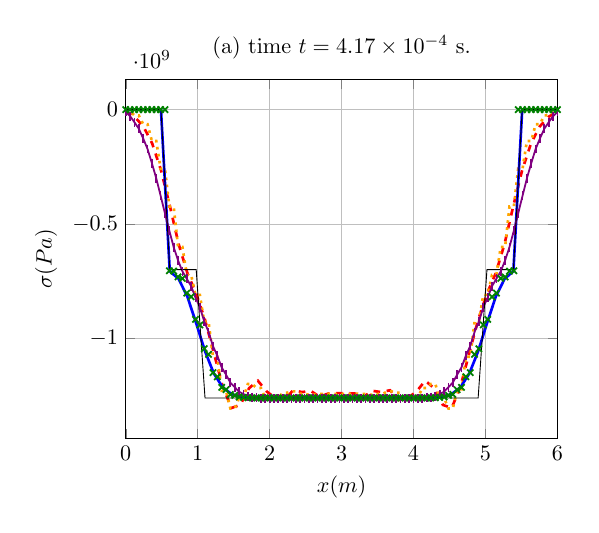
\begin{tikzpicture}[scale=0.8]
\begin{axis}[xlabel=$x (m)$,ylabel=$\sigma (Pa)$,ymajorgrids=true,xmajorgrids=true,legend pos=outer north east,title={(a) time $t = 4.17\times 10^{-4} $ s.},xmin=0.,xmax=6.]
\addplot[Red,very thick,mark=none,dashed] coordinates {(0.0,-8433215.03790355) (0.12244897959183673,-31379937.150059074) (0.24489795918367346,-73325965.87671247) (0.36734693877551017,-147815909.35881704) (0.4897959183673469,-264501011.32373637) (0.6122448979591837,-419797360.6339785) (0.7346938775510203,-586994803.1537646) (0.8571428571428571,-715242874.2277462) (0.9795918367346939,-804731796.1198385) (1.1020408163265305,-919403784.9173691) (1.2244897959183674,-1063504114.033879) (1.346938775510204,-1209904754.949398) (1.4693877551020407,-1304654513.0867395) (1.5918367346938775,-1291382612.5749428) (1.7142857142857142,-1218226204.6353252) (1.836734693877551,-1185455835.0777807) (1.9591836734693877,-1232745182.470082) (2.0816326530612246,-1261396271.0817113) (2.204081632653061,-1270103667.4391637) (2.326530612244898,-1227250869.598082) (2.4489795918367347,-1235273389.504192) (2.571428571428571,-1229787858.686364) (2.693877551020408,-1255621316.42765) (2.816326530612245,-1241442333.7811728) (2.9387755102040813,-1239848703.7218106) (3.061224489795918,-1239848703.7218091) (3.183673469387755,-1241442333.781176) (3.306122448979592,-1255621316.4276485) (3.4285714285714284,-1229787858.6863654) (3.5510204081632653,-1235273389.5041904) (3.673469387755102,-1227250869.598084) (3.7959183673469385,-1270103667.439164) (3.9183673469387754,-1261396271.081712) (4.040816326530612,-1232745182.4700806) (4.163265306122449,-1185455835.0777805) (4.285714285714286,-1218226204.6353254) (4.408163265306122,-1291382612.5749435) (4.530612244897959,-1304654513.0867395) (4.653061224489796,-1209904754.9493968) (4.775510204081632,-1063504114.033878) (4.8979591836734695,-919403784.917369) (5.020408163265306,-804731796.1198374) (5.142857142857142,-715242874.2277458) (5.26530612244898,-586994803.1537648) (5.387755102040816,-419797360.63397753) (5.5102040816326525,-264501011.3237358) (5.63265306122449,-147815909.35881624) (5.755102040816326,-73325965.8767119) (5.877551020408163,-31379937.150058918) (6.0,-8433215.037903389) };
\addplot[Orange,very thick,mark=none,dotted] coordinates {(0.0,-6487195.537951967) (0.06060606060606061,-6487195.537951967) (0.12121212121212122,-25447135.693615116) (0.18181818181818182,-25447135.693615116) (0.24242424242424243,-63824482.75083538) (0.30303030303030304,-63824482.75083538) (0.36363636363636365,-137285465.71899292) (0.42424242424242425,-137285465.71899292) (0.48484848484848486,-258389785.15975574) (0.5454545454545454,-258389785.15975574) (0.6060606060606061,-423881256.5395016) (0.6666666666666667,-423881256.5395016) (0.7272727272727273,-600583024.9453735) (0.7878787878787878,-600583024.9453735) (0.8484848484848485,-722865198.6395395) (0.9090909090909092,-722865198.6395395) (0.9696969696969697,-810023297.3770617) (1.0303030303030303,-810023297.3770617) (1.0909090909090908,-927952236.069318) (1.1515151515151516,-927952236.069318) (1.2121212121212122,-1080376380.893252) (1.2727272727272727,-1080376380.893252) (1.3333333333333335,-1229973271.6895852) (1.393939393939394,-1229973271.6895852) (1.4545454545454546,-1306874646.9216745) (1.5151515151515151,-1306874646.9216745) (1.5757575757575757,-1260590226.5138178) (1.6363636363636365,-1260590226.5138178) (1.696969696969697,-1200189199.3767865) (1.7575757575757576,-1200189199.3767865) (1.8181818181818183,-1217233767.7027068) (1.878787878787879,-1217233767.7027068) (1.9393939393939394,-1260358671.3727095) (2.0,-1260358671.3727095) (2.0606060606060606,-1261618284.922131) (2.121212121212121,-1261618284.922131) (2.1818181818181817,-1238228645.818687) (2.2424242424242427,-1238228645.818687) (2.303030303030303,-1232247837.5911345) (2.3636363636363638,-1232247837.5911345) (2.4242424242424243,-1242565564.7913089) (2.484848484848485,-1242565564.7913089) (2.5454545454545454,-1247187746.3284252) (2.606060606060606,-1247187746.3284252) (2.666666666666667,-1243527207.3601675) (2.7272727272727275,-1243527207.3601675) (2.787878787878788,-1241890915.1682148) (2.8484848484848486,-1241890915.1682148) (2.909090909090909,-1243871775.6139772) (2.9696969696969697,-1243871775.6139772) (3.0303030303030303,-1243871775.613977) (3.090909090909091,-1243871775.613977) (3.1515151515151514,-1241890915.1682146) (3.2121212121212124,-1241890915.1682146) (3.272727272727273,-1243527207.3601675) (3.3333333333333335,-1243527207.3601675) (3.393939393939394,-1247187746.3284254) (3.4545454545454546,-1247187746.3284254) (3.515151515151515,-1242565564.7913094) (3.5757575757575757,-1242565564.7913094) (3.6363636363636367,-1232247837.591135) (3.6969696969696972,-1232247837.591135) (3.757575757575758,-1238228645.818687) (3.8181818181818183,-1238228645.818687) (3.878787878787879,-1261618284.9221313) (3.9393939393939394,-1261618284.9221313) (4.0,-1260358671.37271) (4.0606060606060606,-1260358671.37271) (4.121212121212121,-1217233767.7027078) (4.181818181818182,-1217233767.7027078) (4.242424242424242,-1200189199.3767872) (4.303030303030303,-1200189199.3767872) (4.363636363636363,-1260590226.5138175) (4.424242424242425,-1260590226.5138175) (4.484848484848485,-1306874646.9216745) (4.545454545454546,-1306874646.9216745) (4.606060606060606,-1229973271.6895852) (4.666666666666667,-1229973271.6895852) (4.7272727272727275,-1080376380.893252) (4.787878787878788,-1080376380.893252) (4.848484848484849,-927952236.069318) (4.909090909090909,-927952236.069318) (4.96969696969697,-810023297.3770617) (5.03030303030303,-810023297.3770617) (5.090909090909091,-722865198.6395395) (5.151515151515151,-722865198.6395395) (5.212121212121212,-600583024.9453732) (5.2727272727272725,-600583024.9453732) (5.333333333333334,-423881256.5395015) (5.3939393939393945,-423881256.5395015) (5.454545454545455,-258389785.1597556) (5.515151515151516,-258389785.1597556) (5.575757575757576,-137285465.71899268) (5.636363636363637,-137285465.71899268) (5.696969696969697,-63824482.75083506) (5.757575757575758,-63824482.75083506) (5.818181818181818,-25447135.69361456) (5.878787878787879,-25447135.69361456) (5.9393939393939394,-6487195.537951966) (6.0,-6487195.537951966) };
\addplot[Blue,very thick,mark=none,solid] coordinates {(0.0,-3.2561158711216654e-07) (0.12244897959183673,-6.54162606232603e-22) (0.24489795918367346,0.0) (0.36734693877551017,3.2561158711216643e-07) (0.4897959183673469,-4.884173806682499e-07) (0.6122448979591837,-706703995.0062007) (0.7346938775510203,-739923853.3127105) (0.8571428571428571,-818114621.3278772) (0.9795918367346939,-934350667.0858994) (1.1020408163265305,-1056745717.4113452) (1.2244897959183674,-1153785079.176232) (1.346938775510204,-1213891661.9862223) (1.4693877551020407,-1243675875.166416) (1.5918367346938775,-1255667377.4619899) (1.7142857142857142,-1259628756.7765899) (1.836734693877551,-1260708382.472525) (1.9591836734693877,-1260951555.06527) (2.0816326530612246,-1260996741.6987677) (2.204081632653061,-1261003631.246593) (2.326530612244898,-1261004484.7294881) (2.4489795918367347,-1261004569.3136225) (2.571428571428571,-1261004575.8625927) (2.693877551020408,-1261004576.2443771) (2.816326530612245,-1261004576.2601426) (2.9387755102040813,-1261004576.2605536) (3.061224489795918,-1261004576.2605536) (3.183673469387755,-1261004576.2601426) (3.306122448979592,-1261004576.2443776) (3.4285714285714284,-1261004575.862593) (3.5510204081632653,-1261004569.3136227) (3.673469387755102,-1261004484.7294881) (3.7959183673469385,-1261003631.2465928) (3.9183673469387754,-1260996741.6987677) (4.040816326530612,-1260951555.0652697) (4.163265306122449,-1260708382.4725246) (4.285714285714286,-1259628756.7765894) (4.408163265306122,-1255667377.4619899) (4.530612244897959,-1243675875.1664157) (4.653061224489796,-1213891661.9862223) (4.775510204081632,-1153785079.176232) (4.8979591836734695,-1056745717.4113454) (5.020408163265306,-934350667.0858992) (5.142857142857142,-818114621.327877) (5.26530612244898,-739923853.3127109) (5.387755102040816,-706703995.0062011) (5.5102040816326525,-4.884173806682498e-07) (5.63265306122449,0.0) (5.755102040816326,-4.884173806682498e-07) (5.877551020408163,0.0) (6.0,-4.884173806682498e-07) };
\addplot[Purple,thick,mark=|,solid] coordinates {(0.0,-10397459.452423438) (0.06060606060606061,-28629486.986752886) (0.12121212121212122,-55131928.25663453) (0.18181818181818182,-83646270.11748616) (0.24242424242424243,-125654961.11636907) (0.30303030303030304,-172284594.0778725) (0.36363636363636365,-234043640.37607408) (0.42424242424242425,-300242328.04419184) (0.48484848484848486,-376432798.7765728) (0.5454545454545454,-453818751.237467) (0.6060606060606061,-529414416.2674847) (0.6666666666666667,-601300645.223565) (0.7272727272727273,-659382521.0565735) (0.7878787878787878,-707161316.1944203) (0.8484848484848485,-739803034.1794951) (0.9090909090909092,-772004069.950914) (0.9696969696969697,-822251842.2420584) (1.0303030303030303,-864154645.8439147) (1.0909090909090908,-925876995.0130453) (1.1515151515151516,-972279835.0233293) (1.2121212121212122,-1033743758.8085552) (1.2727272727272727,-1076108794.246372) (1.3333333333333335,-1126940545.3466995) (1.393939393939394,-1158983016.4555871) (1.4545454545454546,-1193843324.3931508) (1.5151515151515151,-1213855388.0055108) (1.5757575757575757,-1233610942.154643) (1.6363636363636365,-1243855259.0681229) (1.696969696969697,-1252984033.6395779) (1.7575757575757576,-1257191611.231863) (1.8181818181818183,-1260529554.0622826) (1.878787878787879,-1261847454.6142046) (1.9393939393939394,-1262731019.2058864) (2.0,-1262988692.0798318) (2.0606060606060606,-1263095211.659083) (2.121212121212121,-1263057284.7251215) (2.1818181818181817,-1263041880.329979) (2.2424242424242427,-1262967457.2713077) (2.303030303030303,-1262995543.9612422) (2.3636363636363638,-1262899504.1699014) (2.4242424242424243,-1262951100.2551603) (2.484848484848485,-1262880485.8465211) (2.5454545454545454,-1262941766.4492297) (2.606060606060606,-1262877340.9880557) (2.666666666666667,-1262975476.3750632) (2.7272727272727275,-1262864851.3501468) (2.787878787878788,-1263076922.0461023) (2.8484848484848486,-1262804308.8537025) (2.909090909090909,-1263257734.3780806) (2.9696969696969697,-1262658504.412126) (3.0303030303030303,-1262658504.4121263) (3.090909090909091,-1263257734.3780804) (3.1515151515151514,-1262804308.8537023) (3.2121212121212124,-1263076922.046102) (3.272727272727273,-1262864851.3501468) (3.3333333333333335,-1262975476.375064) (3.393939393939394,-1262877340.988056) (3.4545454545454546,-1262941766.4492295) (3.515151515151515,-1262880485.8465207) (3.5757575757575757,-1262951100.2551603) (3.6363636363636367,-1262899504.169902) (3.6969696969696972,-1262995543.961243) (3.757575757575758,-1262967457.2713082) (3.8181818181818183,-1263041880.329979) (3.878787878787879,-1263057284.7251215) (3.9393939393939394,-1263095211.6590827) (4.0,-1262988692.0798314) (4.0606060606060606,-1262731019.205886) (4.121212121212121,-1261847454.6142046) (4.181818181818182,-1260529554.0622826) (4.242424242424242,-1257191611.2318633) (4.303030303030303,-1252984033.6395783) (4.363636363636363,-1243855259.0681233) (4.424242424242425,-1233610942.1546435) (4.484848484848485,-1213855388.0055118) (4.545454545454546,-1193843324.3931518) (4.606060606060606,-1158983016.4555879) (4.666666666666667,-1126940545.3467004) (4.7272727272727275,-1076108794.2463727) (4.787878787878788,-1033743758.8085555) (4.848484848484849,-972279835.0233293) (4.909090909090909,-925876995.0130455) (4.96969696969697,-864154645.8439149) (5.03030303030303,-822251842.2420586) (5.090909090909091,-772004069.9509139) (5.151515151515151,-739803034.1794952) (5.212121212121212,-707161316.1944203) (5.2727272727272725,-659382521.0565742) (5.333333333333334,-601300645.2235655) (5.3939393939393945,-529414416.26748544) (5.454545454545455,-453818751.23746747) (5.515151515151516,-376432798.776573) (5.575757575757576,-300242328.0441918) (5.636363636363637,-234043640.37607414) (5.696969696969697,-172284594.0778724) (5.757575757575758,-125654961.1163687) (5.818181818181818,-83646270.11748542) (5.878787878787879,-55131928.256634116) (5.9393939393939394,-28629486.98675295) (6.0,-10397459.452423694) };
\addplot[Green,thick,mark=x,only marks] coordinates {(0.0,-9.938985241112485e-07) (0.06060606060606061,-1.2853825856739185e-06) (0.12121212121212122,8.201488924992559e-07) (0.18181818181818182,4.822974559494094e-07) (0.24242424242424243,-9.83648482392308e-07) (0.30303030303030304,-1.2956326273928566e-06) (0.36363636363636365,1.9586488831001813e-06) (0.42424242424242425,2.5999133364701503e-06) (0.48484848484848486,-1.4790882727589648e-06) (0.5454545454545454,-1.4514160112505328e-06) (0.6060606060606061,-704729842.2455659) (0.6666666666666667,-706002047.1314592) (0.7272727272727273,-731613409.0827894) (0.7878787878787878,-738307360.3254093) (0.8484848484848485,-802443845.4106181) (0.9090909090909092,-818702029.0002648) (0.9696969696969697,-917273418.4084023) (1.0303030303030303,-941457325.3246986) (1.0909090909090908,-1045498983.9435152) (1.1515151515151516,-1070147015.0174686) (1.2121212121212122,-1150104083.776542) (1.2727272727272727,-1168347225.6924338) (1.3333333333333335,-1214623647.0248165) (1.393939393939394,-1224762462.1158886) (1.4545454545454546,-1245337865.7733397) (1.5151515151515151,-1249651955.7951238) (1.5757575757575757,-1256756187.728854) (1.6363636363636365,-1258176137.8011208) (1.696969696969697,-1260087550.9276555) (1.7575757575757576,-1260449997.1780932) (1.8181818181818183,-1260849081.875068) (1.878787878787879,-1260920429.9830258) (1.9393939393939394,-1260984677.091578) (2.0,-1260995458.2161036) (2.0606060606060606,-1261002466.8790119) (2.121212121212121,-1261003454.0601096) (2.1818181818181817,-1261004228.03729) (2.2424242424242427,-1261004332.3287823) (2.303030303030303,-1261004658.4164412) (2.3636363636363638,-1261004353.5092869) (2.4242424242424243,-1261005248.8606844) (2.484848484848485,-1261004976.0401845) (2.5454545454545454,-1261004543.3087149) (2.606060606060606,-1261003848.6940825) (2.666666666666667,-1261005173.6392112) (2.7272727272727275,-1261003422.415637) (2.787878787878788,-1261005964.7480397) (2.8484848484848486,-1261003205.9507174) (2.909090909090909,-1261018212.4618385) (2.9696969696969697,-1260990356.2943678) (3.0303030303030303,-1260990356.2943668) (3.090909090909091,-1261018212.4618378) (3.1515151515151514,-1261003205.950717) (3.2121212121212124,-1261005964.7480397) (3.272727272727273,-1261003422.415637) (3.3333333333333335,-1261005173.6392105) (3.393939393939394,-1261003848.6940827) (3.4545454545454546,-1261004543.3087158) (3.515151515151515,-1261004976.0401855) (3.5757575757575757,-1261005248.860685) (3.6363636363636367,-1261004353.5092869) (3.6969696969696972,-1261004658.4164414) (3.757575757575758,-1261004332.328783) (3.8181818181818183,-1261004228.0372908) (3.878787878787879,-1261003454.0601094) (3.9393939393939394,-1261002466.8790114) (4.0,-1260995458.2161038) (4.0606060606060606,-1260984677.091578) (4.121212121212121,-1260920429.9830256) (4.181818181818182,-1260849081.8750677) (4.242424242424242,-1260449997.1780937) (4.303030303030303,-1260087550.9276562) (4.363636363636363,-1258176137.8011205) (4.424242424242425,-1256756187.728854) (4.484848484848485,-1249651955.795124) (4.545454545454546,-1245337865.7733407) (4.606060606060606,-1224762462.1158893) (4.666666666666667,-1214623647.024817) (4.7272727272727275,-1168347225.692434) (4.787878787878788,-1150104083.7765424) (4.848484848484849,-1070147015.0174688) (4.909090909090909,-1045498983.9435161) (4.96969696969697,-941457325.3246986) (5.03030303030303,-917273418.4084023) (5.090909090909091,-818702029.0002651) (5.151515151515151,-802443845.4106187) (5.212121212121212,-738307360.3254088) (5.2727272727272725,-731613409.0827891) (5.333333333333334,-706002047.1314601) (5.3939393939393945,-704729842.2455676) (5.454545454545455,-9.052507597537938e-07) (5.515151515151516,-7.228071758070392e-07) (5.575757575757576,8.567216523351019e-07) (5.636363636363637,7.713362832257307e-07) (5.696969696969697,-5.847958087280893e-07) (5.757575757575758,-7.176505397205777e-07) (5.818181818181818,1.1498742353244018e-06) (5.878787878787879,1.4550184615729307e-06) (5.9393939393939394,-2.547964815114839e-06) (6.0,-2.336208991567657e-06) };
\addplot[black,thin,mark=none,solid] coordinates {(0.0,-0.0) (0.12244897959183673,-0.0) (0.24489795918367346,-0.0) (0.36734693877551017,-0.0) (0.4897959183673469,-0.0) (0.6122448979591837,-700000000.0) (0.7346938775510203,-700000000.0) (0.8571428571428571,-700000000.0) (0.9795918367346939,-700000000.0) (1.1020408163265305,-1261004576.260559) (1.2244897959183674,-1261004576.260559) (1.346938775510204,-1261004576.260559) (1.4693877551020407,-1261004576.260559) (1.5918367346938775,-1261004576.260559) (1.7142857142857142,-1261004576.260559) (1.836734693877551,-1261004576.260559) (1.9591836734693877,-1261004576.260559) (2.0816326530612246,-1261004576.260559) (2.204081632653061,-1261004576.260559) (2.326530612244898,-1261004576.260559) (2.4489795918367347,-1261004576.260559) (2.571428571428571,-1261004576.260559) (2.693877551020408,-1261004576.260559) (2.816326530612245,-1261004576.260559) (2.9387755102040813,-1261004576.260559) (3.061224489795918,-1261004576.260559) (3.183673469387755,-1261004576.260559) (3.306122448979592,-1261004576.260559) (3.4285714285714284,-1261004576.260559) (3.5510204081632653,-1261004576.260559) (3.673469387755102,-1261004576.260559) (3.7959183673469385,-1261004576.260559) (3.9183673469387754,-1261004576.260559) (4.040816326530612,-1261004576.260559) (4.163265306122449,-1261004576.260559) (4.285714285714286,-1261004576.260559) (4.408163265306122,-1261004576.260559) (4.530612244897959,-1261004576.260559) (4.653061224489796,-1261004576.260559) (4.775510204081632,-1261004576.260559) (4.8979591836734695,-1261004576.260559) (5.020408163265306,-700000000.0) (5.142857142857142,-700000000.0) (5.26530612244898,-700000000.0) (5.387755102040816,-700000000.0) (5.5102040816326525,-0.0) (5.63265306122449,-0.0) (5.755102040816326,-0.0) (5.877551020408163,-0.0) (6.0,-0.0) };
%\legend{usl 1ppc,usl 2ppc,dgmpm 1ppc,dgmpm 2ppc,dgmpm 2ppc (RK2),exact}
\end{axis}
\end{tikzpicture}
%%% Local Variables:
%%% mode: latex
%%% TeX-master: "../../mainManuscript"
%%% End:
}
%   % {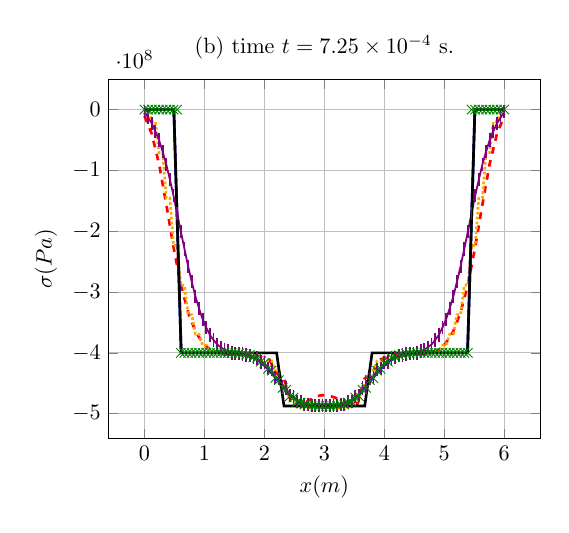
\begin{tikzpicture}[scale=0.8]
\begin{axis}[xlabel=$x (m)$,ylabel=$\sigma (Pa)$,ymajorgrids=true,xmajorgrids=true,legend pos=outer north east,title={(b) time $t = 7.25\times 10^{-4} $ s.}]
\addplot[Red,very thick,mark=none,dashed,mark size=3pt] coordinates {(0.0,-10477027.22040739) (0.12244897959183673,-40202439.77672757) (0.24489795918367346,-90268409.98400429) (0.36734693877551017,-157917330.96394995) (0.4897959183673469,-229098117.24026006) (0.6122448979591837,-290170966.79273176) (0.7346938775510203,-335449952.79523534) (0.8571428571428571,-366063963.8356788) (0.9795918367346939,-384934670.81956863) (1.1020408163265305,-394978768.22705775) (1.2244897959183674,-399539747.49342227) (1.346938775510204,-401064801.98949975) (1.4693877551020407,-401261686.3649931) (1.5918367346938775,-401362011.1717392) (1.7142857142857142,-402125702.7814173) (1.836734693877551,-402648608.50963366) (1.9591836734693877,-407517028.59914577) (2.0816326530612246,-411133976.99807984) (2.204081632653061,-433339939.374477) (2.326530612244898,-442099776.2163934) (2.4489795918367347,-483576545.68129754) (2.571428571428571,-481854124.4484605) (2.693877551020408,-481095256.73223835) (2.816326530612245,-473792554.1947772) (2.9387755102040813,-469732138.6842222) (3.061224489795918,-469732138.6842212) (3.183673469387755,-473792554.1947779) (3.306122448979592,-481095256.73223734) (3.4285714285714284,-481854124.4484616) (3.5510204081632653,-483576545.6812961) (3.673469387755102,-442099776.2163934) (3.7959183673469385,-433339939.3744765) (3.9183673469387754,-411133976.99807984) (4.040816326530612,-407517028.5991456) (4.163265306122449,-402648608.50963354) (4.285714285714286,-402125702.78141725) (4.408163265306122,-401362011.1717393) (4.530612244897959,-401261686.3649931) (4.653061224489796,-401064801.9894998) (4.775510204081632,-399539747.4934223) (4.8979591836734695,-394978768.22705775) (5.020408163265306,-384934670.81956846) (5.142857142857142,-366063963.83567846) (5.26530612244898,-335449952.79523504) (5.387755102040816,-290170966.7927308) (5.5102040816326525,-229098117.24025902) (5.63265306122449,-157917330.96394882) (5.755102040816326,-90268409.98400334) (5.877551020408163,-40202439.77672676) (6.0,-10477027.22040709) };
\addplot[Orange,very thick,mark=none,densely dotted,mark size=3pt] coordinates {(0.0,-1522322.3567553319) (0.06060606060606061,-1522322.3567553319) (0.12121212121212122,-19741546.758713853) (0.18181818181818182,-19741546.758713853) (0.24242424242424243,-70452847.74734518) (0.30303030303030304,-70452847.74734518) (0.36363636363636365,-145569726.72165304) (0.42424242424242425,-145569726.72165304) (0.48484848484848486,-223558621.35896367) (0.5454545454545454,-223558621.35896367) (0.6060606060606061,-288852526.8705149) (0.6666666666666667,-288852526.8705149) (0.7272727272727273,-337120167.47142065) (0.7878787878787878,-337120167.47142065) (0.8484848484848485,-369182466.2528492) (0.9090909090909092,-369182466.2528492) (0.9696969696969697,-387695734.7050902) (1.0303030303030303,-387695734.7050902) (1.0909090909090908,-396787746.7545124) (1.1515151515151516,-396787746.7545124) (1.2121212121212122,-400346482.5664338) (1.2727272727272727,-400346482.5664338) (1.3333333333333335,-401071106.301628) (1.393939393939394,-401071106.301628) (1.4545454545454546,-401189158.25601304) (1.5151515151515151,-401189158.25601304) (1.5757575757575757,-401411626.48080814) (1.6363636363636365,-401411626.48080814) (1.696969696969697,-401847412.82243955) (1.7575757575757576,-401847412.82243955) (1.8181818181818183,-402892812.90166867) (1.878787878787879,-402892812.90166867) (1.9393939393939394,-405871331.09740126) (2.0,-405871331.09740126) (2.0606060606060606,-413271912.46434987) (2.121212121212121,-413271912.46434987) (2.1818181818181817,-428650643.90280265) (2.2424242424242427,-428650643.90280265) (2.303030303030303,-453302573.20518476) (2.3636363636363638,-453302573.20518476) (2.4242424242424243,-478258276.212825) (2.484848484848485,-478258276.212825) (2.5454545454545454,-489476664.1834195) (2.606060606060606,-489476664.1834195) (2.666666666666667,-489046885.64068294) (2.7272727272727275,-489046885.64068294) (2.787878787878788,-491447894.73413926) (2.8484848484848486,-491447894.73413926) (2.909090909090909,-486436945.7103945) (2.9696969696969697,-486436945.7103945) (3.0303030303030303,-486436945.7103945) (3.090909090909091,-486436945.7103945) (3.1515151515151514,-491447894.73413926) (3.2121212121212124,-491447894.73413926) (3.272727272727273,-489046885.64068294) (3.3333333333333335,-489046885.64068294) (3.393939393939394,-489476664.1834195) (3.4545454545454546,-489476664.1834195) (3.515151515151515,-478258276.212825) (3.5757575757575757,-478258276.212825) (3.6363636363636367,-453302573.2051846) (3.6969696969696972,-453302573.2051846) (3.757575757575758,-428650643.9028025) (3.8181818181818183,-428650643.9028025) (3.878787878787879,-413271912.46434987) (3.9393939393939394,-413271912.46434987) (4.0,-405871331.09740126) (4.0606060606060606,-405871331.09740126) (4.121212121212121,-402892812.90166855) (4.181818181818182,-402892812.90166855) (4.242424242424242,-401847412.82243955) (4.303030303030303,-401847412.82243955) (4.363636363636363,-401411626.4808081) (4.424242424242425,-401411626.4808081) (4.484848484848485,-401189158.25601304) (4.545454545454546,-401189158.25601304) (4.606060606060606,-401071106.3016279) (4.666666666666667,-401071106.3016279) (4.7272727272727275,-400346482.5664337) (4.787878787878788,-400346482.5664337) (4.848484848484849,-396787746.75451225) (4.909090909090909,-396787746.75451225) (4.96969696969697,-387695734.7050903) (5.03030303030303,-387695734.7050903) (5.090909090909091,-369182466.25284934) (5.151515151515151,-369182466.25284934) (5.212121212121212,-337120167.47142065) (5.2727272727272725,-337120167.47142065) (5.333333333333334,-288852526.8705149) (5.3939393939393945,-288852526.8705149) (5.454545454545455,-223558621.35896364) (5.515151515151516,-223558621.35896364) (5.575757575757576,-145569726.72165304) (5.636363636363637,-145569726.72165304) (5.696969696969697,-70452847.74734521) (5.757575757575758,-70452847.74734521) (5.818181818181818,-19741546.758713897) (5.878787878787879,-19741546.758713897) (5.9393939393939394,-1522322.3567553656) (6.0,-1522322.3567553656) };
\addplot[Blue,very thick,mark=none,solid,mark size=3pt] coordinates {(0.0,-0.016398596440346053) (0.12244897959183673,-0.06425322857955201) (0.24489795918367346,-0.7380674881804443) (0.36734693877551017,-2.12047390173559) (0.4897959183673469,-28.76271861558054) (0.6122448979591837,-400000015.4159754) (0.7346938775510203,-400000102.7573024) (0.8571428571428571,-400000598.1932516) (0.9795918367346939,-400003055.79803795) (1.1020408163265305,-400013747.0436081) (1.2244897959183674,-400054602.7199052) (1.346938775510204,-400191823.2382515) (1.4693877551020407,-400596672.6802674) (1.5918367346938775,-401644186.51493835) (1.7142857142857142,-404014374.4754996) (1.836734693877551,-408684632.25449073) (1.9591836734693877,-416652037.9726774) (2.0816326530612246,-428329061.0045163) (2.204081632653061,-442879954.5361007) (2.326530612244898,-458084443.80872595) (2.4489795918367347,-471157539.9020842) (2.571428571428571,-480164339.19475454) (2.693877551020408,-484944715.5259052) (2.816326530612245,-486779650.5319825) (2.9387755102040813,-487233015.60471344) (3.061224489795918,-487233015.60471344) (3.183673469387755,-486779650.5319825) (3.306122448979592,-484944715.5259052) (3.4285714285714284,-480164339.19475454) (3.5510204081632653,-471157539.9020842) (3.673469387755102,-458084443.80872613) (3.7959183673469385,-442879954.5361007) (3.9183673469387754,-428329061.0045163) (4.040816326530612,-416652037.9726776) (4.163265306122449,-408684632.2544908) (4.285714285714286,-404014374.4754996) (4.408163265306122,-401644186.5149382) (4.530612244897959,-400596672.68026733) (4.653061224489796,-400191823.2382513) (4.775510204081632,-400054602.7199051) (4.8979591836734695,-400013747.04360807) (5.020408163265306,-400003055.79803795) (5.142857142857142,-400000598.19325155) (5.26530612244898,-400000102.75730234) (5.387755102040816,-400000015.4159754) (5.5102040816326525,-28.762718512303003) (5.63265306122449,-2.1204742438100417) (5.755102040816326,-0.7380675867576459) (5.877551020408163,-0.06425320166977637) (6.0,-0.01639854380134023) };
\addplot[Purple,thick,mark=|,solid,mark size=3pt] coordinates {(0.0,-3643722.4057531543) (0.06060606060606061,-13253871.94771175) (0.12121212121212122,-22430884.29879855) (0.18181818181818182,-35710388.05852378) (0.24242424242424243,-49954062.55465116) (0.30303030303030304,-69199724.63429566) (0.36363636363636365,-90001064.05703217) (0.42424242424242425,-115227809.11229268) (0.48484848484848486,-141771114.02793142) (0.5454545454545454,-170682311.90803242) (0.6060606060606061,-200079540.00258502) (0.6666666666666667,-229014826.8013297) (0.7272727272727273,-257430278.9843493) (0.7878787878787878,-282843592.21811193) (0.8484848484848485,-306971268.4010445) (0.9090909090909092,-326667104.7497092) (0.9696969696969697,-344782488.29979676) (1.0303030303030303,-358341830.7310785) (1.0909090909090908,-370462827.7146289) (1.1515151515151516,-378821810.49726343) (1.2121212121212122,-386102976.6619535) (1.2727272727272727,-390706555.81264853) (1.3333333333333335,-394846891.2394369) (1.393939393939394,-396879468.6459066) (1.4545454545454546,-400395334.89461267) (1.5151515151515151,-400547253.1901776) (1.5757575757575757,-401393994.5226969) (1.6363636363636365,-401653877.80383056) (1.696969696969697,-403469259.9494932) (1.7575757575757576,-403991527.1056523) (1.8181818181818183,-407625905.94533336) (1.878787878787879,-408563059.4680144) (1.9393939393939394,-414922856.8689467) (2.0,-416374885.2462252) (2.0606060606060606,-425987877.61701065) (2.121212121212121,-427906862.049074) (2.1818181818181817,-440309840.98849624) (2.2424242424242427,-442439362.1915814) (2.303030303030303,-455885132.24318355) (2.3636363636363638,-457826856.56220615) (2.4242424242424243,-469809715.6908375) (2.484848484848485,-471219084.61224025) (2.5454545454545454,-479722411.6158245) (2.606060606060606,-480495963.9518887) (2.666666666666667,-485058185.3772167) (2.7272727272727275,-485348110.0144077) (2.787878787878788,-487020339.6946885) (2.8484848484848486,-487075458.5679951) (2.909090909090909,-487055267.13670456) (2.9696969696969697,-486361892.7822711) (3.0303030303030303,-486361892.78227144) (3.090909090909091,-487055267.1367042) (3.1515151515151514,-487075458.5679951) (3.2121212121212124,-487020339.69468886) (3.272727272727273,-485348110.0144077) (3.3333333333333335,-485058185.37721705) (3.393939393939394,-480495963.9518887) (3.4545454545454546,-479722411.6158245) (3.515151515151515,-471219084.61224025) (3.5757575757575757,-469809715.6908375) (3.6363636363636367,-457826856.5622063) (3.6969696969696972,-455885132.24318355) (3.757575757575758,-442439362.1915814) (3.8181818181818183,-440309840.98849636) (3.878787878787879,-427906862.0490741) (3.9393939393939394,-425987877.6170107) (4.0,-416374885.2462253) (4.0606060606060606,-414922856.86894685) (4.121212121212121,-408563059.46801454) (4.181818181818182,-407625905.94533336) (4.242424242424242,-403991527.1056523) (4.303030303030303,-403469259.9494934) (4.363636363636363,-401653877.80383074) (4.424242424242425,-401393994.522697) (4.484848484848485,-400547253.19017774) (4.545454545454546,-400395334.89461285) (4.606060606060606,-396879468.6459065) (4.666666666666667,-394846891.23943704) (4.7272727272727275,-390706555.81264836) (4.787878787878788,-386102976.66195333) (4.848484848484849,-378821810.4972633) (4.909090909090909,-370462827.71462864) (4.96969696969697,-358341830.73107857) (5.03030303030303,-344782488.29979694) (5.090909090909091,-326667104.7497094) (5.151515151515151,-306971268.4010446) (5.212121212121212,-282843592.21811193) (5.2727272727272725,-257430278.98434916) (5.333333333333334,-229014826.8013294) (5.3939393939393945,-200079540.00258464) (5.454545454545455,-170682311.90803197) (5.515151515151516,-141771114.0279309) (5.575757575757576,-115227809.11229216) (5.636363636363637,-90001064.0570316) (5.696969696969697,-69199724.63429512) (5.757575757575758,-49954062.55465064) (5.818181818181818,-35710388.058523305) (5.878787878787879,-22430884.29879819) (5.9393939393939394,-13253871.947711527) (6.0,-3643722.4057530854) };
\addplot[Green,thin,mark=x,only marks,mark size=3pt] coordinates {(0.0,-0.0009905544907868183) (0.06060606060606061,-0.001035109508555422) (0.12121212121212122,-0.005117191018500656) (0.18181818181818182,-0.0052978434023460315) (0.24242424242424243,-0.06517986204950546) (0.30303030303030304,-0.07566277987844348) (0.36363636363636365,-0.24962042121048697) (0.42424242424242425,-0.26937038060136104) (0.48484848484848486,-3.010621421655401) (0.5454545454545454,-5.186761151690843) (0.6060606060606061,-400000002.01453906) (0.6666666666666667,-400000003.4473042) (0.7272727272727273,-400000017.3967542) (0.7878787878787878,-400000028.78236) (0.8484848484848485,-400000129.15230495) (0.9090909090909092,-400000206.4599203) (0.9696969696969697,-400000827.7884989) (1.0303030303030303,-400001277.7907757) (1.0909090909090908,-400004594.5128382) (1.1515151515151516,-400006844.3811263) (1.2121212121212122,-400022128.58005637) (1.2727272727272727,-400031796.16010183) (1.3333333333333335,-400092597.4804089) (1.393939393939394,-400128278.6945615) (1.4545454545454546,-400336842.6530185) (1.5151515151515151,-400449754.98737735) (1.5757575757575757,-401065298.1117383) (1.6363636363636365,-401370713.3108358) (1.696969696969697,-402928435.1963118) (1.7575757575757576,-403631417.36330265) (1.8181818181818183,-406995518.8189568) (1.878787878787879,-408364026.9334509) (1.9393939393939394,-414524891.6433188) (2.0,-416759867.3744382) (2.0606060606060606,-426248412.6400655) (2.121212121212121,-429277915.8940706) (2.1818181818181817,-441434961.5049247) (2.2424242424242427,-444795234.23076177) (2.303030303030303,-457568597.61163) (2.3636363636363638,-460560432.82157856) (2.4242424242424243,-471355976.94533) (2.484848484848485,-473437539.61930424) (2.5454545454545454,-480581531.6160863) (2.606060606060606,-481669280.4693011) (2.666666666666667,-485226958.9355893) (2.7272727272727275,-485627667.237451) (2.787878787878788,-486879003.35388845) (2.8484848484848486,-486971605.60944414) (2.909090909090909,-487248222.53163636) (2.9696969696969697,-487258302.19873005) (3.0303030303030303,-487258302.19873005) (3.090909090909091,-487248222.53163636) (3.1515151515151514,-486971605.60944414) (3.2121212121212124,-486879003.35388845) (3.272727272727273,-485627667.237451) (3.3333333333333335,-485226958.9355893) (3.393939393939394,-481669280.4693011) (3.4545454545454546,-480581531.6160863) (3.515151515151515,-473437539.6193044) (3.5757575757575757,-471355976.94533) (3.6363636363636367,-460560432.82157856) (3.6969696969696972,-457568597.61163) (3.757575757575758,-444795234.23076177) (3.8181818181818183,-441434961.5049247) (3.878787878787879,-429277915.8940706) (3.9393939393939394,-426248412.64006543) (4.0,-416759867.3744382) (4.0606060606060606,-414524891.64331895) (4.121212121212121,-408364026.933451) (4.181818181818182,-406995518.8189568) (4.242424242424242,-403631417.3633025) (4.303030303030303,-402928435.1963118) (4.363636363636363,-401370713.3108358) (4.424242424242425,-401065298.11173844) (4.484848484848485,-400449754.9873774) (4.545454545454546,-400336842.65301853) (4.606060606060606,-400128278.6945615) (4.666666666666667,-400092597.48040897) (4.7272727272727275,-400031796.16010183) (4.787878787878788,-400022128.5800565) (4.848484848484849,-400006844.3811263) (4.909090909090909,-400004594.51283836) (4.96969696969697,-400001277.7907758) (5.03030303030303,-400000827.7884989) (5.090909090909091,-400000206.4599203) (5.151515151515151,-400000129.152305) (5.212121212121212,-400000028.7823601) (5.2727272727272725,-400000017.39675426) (5.333333333333334,-400000003.4473042) (5.3939393939393945,-400000002.014539) (5.454545454545455,-5.186761729700046) (5.515151515151516,-3.0106210293278775) (5.575757575757576,-0.26937051997179645) (5.636363636363637,-0.249620419252184) (5.696969696969697,-0.07566313892965675) (5.757575757575758,-0.06517962792185199) (5.818181818181818,-0.00529745130538514) (5.878787878787879,-0.005117314055782253) (5.9393939393939394,-0.0010346801603060291) (6.0,-0.0009902966227138578) };
\addplot[black,very thick,mark=pentagone*,solid,mark size=3pt] coordinates {(0.0,-0.0) (0.12244897959183673,-0.0) (0.24489795918367346,-0.0) (0.36734693877551017,-0.0) (0.4897959183673469,-0.0) (0.6122448979591837,-400000000.0) (0.7346938775510203,-400000000.0) (0.8571428571428571,-400000000.0) (0.9795918367346939,-400000000.0) (1.1020408163265305,-400000000.0) (1.2244897959183674,-400000000.0) (1.346938775510204,-400000000.0) (1.4693877551020407,-400000000.0) (1.5918367346938775,-400000000.0) (1.7142857142857142,-400000000.0) (1.836734693877551,-400000000.0) (1.9591836734693877,-400000000.0) (2.0816326530612246,-400000000.0) (2.204081632653061,-400000000.0) (2.326530612244898,-487287156.09439695) (2.4489795918367347,-487287156.09439695) (2.571428571428571,-487287156.09439695) (2.693877551020408,-487287156.09439695) (2.816326530612245,-487287156.09439695) (2.9387755102040813,-487287156.09439695) (3.061224489795918,-487287156.09439695) (3.183673469387755,-487287156.09439695) (3.306122448979592,-487287156.09439695) (3.4285714285714284,-487287156.09439695) (3.5510204081632653,-487287156.09439695) (3.673469387755102,-487287156.09439695) (3.7959183673469385,-400000000.0) (3.9183673469387754,-400000000.0) (4.040816326530612,-400000000.0) (4.163265306122449,-400000000.0) (4.285714285714286,-400000000.0) (4.408163265306122,-400000000.0) (4.530612244897959,-400000000.0) (4.653061224489796,-400000000.0) (4.775510204081632,-400000000.0) (4.8979591836734695,-400000000.0) (5.020408163265306,-400000000.0) (5.142857142857142,-400000000.0) (5.26530612244898,-400000000.0) (5.387755102040816,-400000000.0) (5.5102040816326525,-0.0) (5.63265306122449,-0.0) (5.755102040816326,-0.0) (5.877551020408163,-0.0) (6.0,-0.0) };
%\legend{usl 1ppc,usl 2ppc,dgmpm 1ppc,dgmpm 2ppc,dgmpm 2ppc (RK2),exact}
\end{axis}
\end{tikzpicture}
%%% Local Variables:
%%% mode: latex
%%% TeX-master: "../../mainManuscript"
%%% End:
}
%   {\begin{tikzpicture}[scale=.9]
\begin{groupplot}[group style={group size=3 by 2,
ylabels at=edge left, yticklabels at=edge left,horizontal sep=2.ex,
vertical sep=4ex,xticklabels at=edge bottom,xlabels at=edge bottom},
ymajorgrids=true,xmajorgrids=true,enlargelimits=0,xmin=0.,xmax=6.,xlabel=$x (m)$,
axis on top,scale only axis,width=0.32\linewidth
]
\nextgroupplot[title={(a) $t = 4.17\times 10^{-4} $ s.},ylabel=$\sigma (Pa)$,]
\addplot[Blue,solid,mark=none,very thick,mark size=2pt] coordinates{(0.0,-3.25611587112e-07) (0.122448979592,-6.54162606233e-22) (0.244897959184,0.0) (0.367346938776,3.25611587112e-07) (0.489795918367,-4.88417380668e-07) (0.612244897959,-706703995.006) (0.734693877551,-739923853.313) (0.857142857143,-818114621.328) (0.979591836735,-934350667.086) (1.10204081633,-1056745717.41) (1.22448979592,-1153785079.18) (1.34693877551,-1213891661.99) (1.4693877551,-1243675875.17) (1.59183673469,-1255667377.46) (1.71428571429,-1259628756.78) (1.83673469388,-1260708382.47) (1.95918367347,-1260951555.07) (2.08163265306,-1260996741.7) (2.20408163265,-1261003631.25) (2.32653061224,-1261004484.73) (2.44897959184,-1261004569.31) (2.57142857143,-1261004575.86) (2.69387755102,-1261004576.24) (2.81632653061,-1261004576.26) (2.9387755102,-1261004576.26) (3.0612244898,-1261004576.26) (3.18367346939,-1261004576.26) (3.30612244898,-1261004576.24) (3.42857142857,-1261004575.86) (3.55102040816,-1261004569.31) (3.67346938776,-1261004484.73) (3.79591836735,-1261003631.25) (3.91836734694,-1260996741.7) (4.04081632653,-1260951555.07) (4.16326530612,-1260708382.47) (4.28571428571,-1259628756.78) (4.40816326531,-1255667377.46) (4.5306122449,-1243675875.17) (4.65306122449,-1213891661.99) (4.77551020408,-1153785079.18) (4.89795918367,-1056745717.41) (5.02040816327,-934350667.086) (5.14285714286,-818114621.328) (5.26530612245,-739923853.313) (5.38775510204,-706703995.006) (5.51020408163,-4.88417380668e-07) (5.63265306122,0.0) (5.75510204082,-4.88417380668e-07) (5.87755102041,0.0) (6.0,-4.88417380668e-07) };
\addplot[Purple,only marks,mark=+,thin,mark size=2pt] coordinates{(0.0,-6327912.39976) (0.0606060606061,-17393855.4498) (0.121212121212,-34791452.0156) (0.181818181818,-54271429.8986) (0.242424242424,-85476186.7634) (0.30303030303,-121344975.529) (0.363636363636,-172772413.109) (0.424242424242,-229646809.33) (0.484848484848,-300604808.871) (0.545454545455,-374985968.406) (0.606060606061,-454379573.056) (0.666666666667,-532582620.671) (0.727272727273,-601889718.545) (0.787878787879,-665111214.747) (0.848484848485,-710389190.246) (0.909090909091,-740809726.393) (0.969696969697,-783840999.734) (1.0303030303,-822574838.477) (1.09090909091,-881869005.613) (1.15151515152,-928117392.832) (1.21212121212,-992030440.922) (1.27272727273,-1037630664.81) (1.33333333333,-1094332999.9) (1.39393939394,-1131243116.44) (1.45454545455,-1172779891.01) (1.51515151515,-1197412378.63) (1.57575757576,-1222494297.05) (1.63636363636,-1235925009.98) (1.69696969697,-1248261695.93) (1.75757575758,-1254152813.68) (1.81818181818,-1258986167.93) (1.87878787879,-1260986849.61) (1.93939393939,-1262401857.25) (2.0,-1262863321.6) (2.06060606061,-1263097274.85) (2.12121212121,-1263105090.64) (2.18181818182,-1263091292.13) (2.24242424242,-1263006777.33) (2.30303030303,-1263028365.67) (2.36363636364,-1262931396.23) (2.42424242424,-1262985011.95) (2.48484848485,-1262917562.75) (2.54545454545,-1262983412.75) (2.60606060606,-1262924149.66) (2.66666666667,-1263029713.54) (2.72727272727,-1262927168.66) (2.78787878788,-1263147911.39) (2.84848484848,-1262880892.07) (2.90909090909,-1263338476.16) (2.9696969697,-1262740516.98) (3.0303030303,-1262740516.98) (3.09090909091,-1263338476.16) (3.15151515152,-1262880892.07) (3.21212121212,-1263147911.39) (3.27272727273,-1262927168.66) (3.33333333333,-1263029713.54) (3.39393939394,-1262924149.66) (3.45454545455,-1262983412.75) (3.51515151515,-1262917562.75) (3.57575757576,-1262985011.95) (3.63636363636,-1262931396.23) (3.69696969697,-1263028365.67) (3.75757575758,-1263006777.33) (3.81818181818,-1263091292.13) (3.87878787879,-1263105090.64) (3.93939393939,-1263097274.85) (4.0,-1262863321.6) (4.06060606061,-1262401857.25) (4.12121212121,-1260986849.61) (4.18181818182,-1258986167.93) (4.24242424242,-1254152813.68) (4.30303030303,-1248261695.93) (4.36363636364,-1235925009.98) (4.42424242424,-1222494297.05) (4.48484848485,-1197412378.63) (4.54545454545,-1172779891.01) (4.60606060606,-1131243116.44) (4.66666666667,-1094332999.9) (4.72727272727,-1037630664.81) (4.78787878788,-992030440.922) (4.84848484848,-928117392.832) (4.90909090909,-881869005.613) (4.9696969697,-822574838.477) (5.0303030303,-783840999.734) (5.09090909091,-740809726.393) (5.15151515152,-710389190.246) (5.21212121212,-665111214.747) (5.27272727273,-601889718.545) (5.33333333333,-532582620.671) (5.39393939394,-454379573.056) (5.45454545455,-374985968.406) (5.51515151515,-300604808.871) (5.57575757576,-229646809.33) (5.63636363636,-172772413.109) (5.69696969697,-121344975.529) (5.75757575758,-85476186.7634) (5.81818181818,-54271429.8986) (5.87878787879,-34791452.0156) (5.93939393939,-17393855.4498) (6.0,-6327912.39976) };
\addplot[Duck,only marks,mark=x,thick,mark size=2pt] coordinates{(0.0,-9.93898524111e-07) (0.0606060606061,-1.28538258567e-06) (0.121212121212,8.20148892499e-07) (0.181818181818,4.82297455949e-07) (0.242424242424,-9.83648482392e-07) (0.30303030303,-1.29563262739e-06) (0.363636363636,1.9586488831e-06) (0.424242424242,2.59991333647e-06) (0.484848484848,-1.47908827276e-06) (0.545454545455,-1.45141601125e-06) (0.606060606061,-704729842.246) (0.666666666667,-706002047.131) (0.727272727273,-731613409.083) (0.787878787879,-738307360.325) (0.848484848485,-802443845.411) (0.909090909091,-818702029.0) (0.969696969697,-917273418.408) (1.0303030303,-941457325.325) (1.09090909091,-1045498983.94) (1.15151515152,-1070147015.02) (1.21212121212,-1150104083.78) (1.27272727273,-1168347225.69) (1.33333333333,-1214623647.02) (1.39393939394,-1224762462.12) (1.45454545455,-1245337865.77) (1.51515151515,-1249651955.8) (1.57575757576,-1256756187.73) (1.63636363636,-1258176137.8) (1.69696969697,-1260087550.93) (1.75757575758,-1260449997.18) (1.81818181818,-1260849081.88) (1.87878787879,-1260920429.98) (1.93939393939,-1260984677.09) (2.0,-1260995458.22) (2.06060606061,-1261002466.88) (2.12121212121,-1261003454.06) (2.18181818182,-1261004228.04) (2.24242424242,-1261004332.33) (2.30303030303,-1261004658.42) (2.36363636364,-1261004353.51) (2.42424242424,-1261005248.86) (2.48484848485,-1261004976.04) (2.54545454545,-1261004543.31) (2.60606060606,-1261003848.69) (2.66666666667,-1261005173.64) (2.72727272727,-1261003422.42) (2.78787878788,-1261005964.75) (2.84848484848,-1261003205.95) (2.90909090909,-1261018212.46) (2.9696969697,-1260990356.29) (3.0303030303,-1260990356.29) (3.09090909091,-1261018212.46) (3.15151515152,-1261003205.95) (3.21212121212,-1261005964.75) (3.27272727273,-1261003422.42) (3.33333333333,-1261005173.64) (3.39393939394,-1261003848.69) (3.45454545455,-1261004543.31) (3.51515151515,-1261004976.04) (3.57575757576,-1261005248.86) (3.63636363636,-1261004353.51) (3.69696969697,-1261004658.42) (3.75757575758,-1261004332.33) (3.81818181818,-1261004228.04) (3.87878787879,-1261003454.06) (3.93939393939,-1261002466.88) (4.0,-1260995458.22) (4.06060606061,-1260984677.09) (4.12121212121,-1260920429.98) (4.18181818182,-1260849081.88) (4.24242424242,-1260449997.18) (4.30303030303,-1260087550.93) (4.36363636364,-1258176137.8) (4.42424242424,-1256756187.73) (4.48484848485,-1249651955.8) (4.54545454545,-1245337865.77) (4.60606060606,-1224762462.12) (4.66666666667,-1214623647.02) (4.72727272727,-1168347225.69) (4.78787878788,-1150104083.78) (4.84848484848,-1070147015.02) (4.90909090909,-1045498983.94) (4.9696969697,-941457325.325) (5.0303030303,-917273418.408) (5.09090909091,-818702029.0) (5.15151515152,-802443845.411) (5.21212121212,-738307360.325) (5.27272727273,-731613409.083) (5.33333333333,-706002047.131) (5.39393939394,-704729842.246) (5.45454545455,-9.05250759754e-07) (5.51515151515,-7.22807175807e-07) (5.57575757576,8.56721652335e-07) (5.63636363636,7.71336283226e-07) (5.69696969697,-5.84795808728e-07) (5.75757575758,-7.17650539721e-07) (5.81818181818,1.14987423532e-06) (5.87878787879,1.45501846157e-06) (5.93939393939,-2.54796481511e-06) (6.0,-2.33620899157e-06) };
\addplot[black,solid,mark=none,thin,mark size=2pt] coordinates{(0.0,-0.0) (0.122448979592,-0.0) (0.244897959184,-0.0) (0.367346938776,-0.0) (0.489795918367,-0.0) (0.612244897959,-700000000.0) (0.734693877551,-700000000.0) (0.857142857143,-700000000.0) (0.979591836735,-700000000.0) (1.10204081633,-1261004576.26) (1.22448979592,-1261004576.26) (1.34693877551,-1261004576.26) (1.4693877551,-1261004576.26) (1.59183673469,-1261004576.26) (1.71428571429,-1261004576.26) (1.83673469388,-1261004576.26) (1.95918367347,-1261004576.26) (2.08163265306,-1261004576.26) (2.20408163265,-1261004576.26) (2.32653061224,-1261004576.26) (2.44897959184,-1261004576.26) (2.57142857143,-1261004576.26) (2.69387755102,-1261004576.26) (2.81632653061,-1261004576.26) (2.9387755102,-1261004576.26) (3.0612244898,-1261004576.26) (3.18367346939,-1261004576.26) (3.30612244898,-1261004576.26) (3.42857142857,-1261004576.26) (3.55102040816,-1261004576.26) (3.67346938776,-1261004576.26) (3.79591836735,-1261004576.26) (3.91836734694,-1261004576.26) (4.04081632653,-1261004576.26) (4.16326530612,-1261004576.26) (4.28571428571,-1261004576.26) (4.40816326531,-1261004576.26) (4.5306122449,-1261004576.26) (4.65306122449,-1261004576.26) (4.77551020408,-1261004576.26) (4.89795918367,-1261004576.26) (5.02040816327,-700000000.0) (5.14285714286,-700000000.0) (5.26530612245,-700000000.0) (5.38775510204,-700000000.0) (5.51020408163,-0.0) (5.63265306122,-0.0) (5.75510204082,-0.0) (5.87755102041,-0.0) (6.0,-0.0) };
\nextgroupplot[title={(b) $t = 6.25\times 10^{-4} $ s.},]
\addplot[Blue,solid,mark=none,very thick,mark size=2pt] coordinates{(0.0,-120597397.192) (0.122448979592,-298539345.155) (0.244897959184,-464504460.171) (0.367346938776,-546627376.356) (0.489795918367,-635546108.254) (0.612244897959,-1247334335.33) (0.734693877551,-1255980074.6) (0.857142857143,-1259371705.53) (0.979591836735,-1260535220.13) (1.10204081633,-1260885267.5) (1.22448979592,-1260977777.71) (1.34693877551,-1260999265.66) (1.4693877551,-1261003650.04) (1.59183673469,-1261004434.57) (1.71428571429,-1261004557.34) (1.83673469388,-1261004574.07) (1.95918367347,-1261004576.04) (2.08163265306,-1261004576.24) (2.20408163265,-1261004576.26) (2.32653061224,-1261004576.26) (2.44897959184,-1261004576.26) (2.57142857143,-1261004576.26) (2.69387755102,-1261004576.26) (2.81632653061,-1261004576.26) (2.9387755102,-1261004576.26) (3.0612244898,-1261004576.26) (3.18367346939,-1261004576.26) (3.30612244898,-1261004576.26) (3.42857142857,-1261004576.26) (3.55102040816,-1261004576.26) (3.67346938776,-1261004576.26) (3.79591836735,-1261004576.26) (3.91836734694,-1261004576.24) (4.04081632653,-1261004576.04) (4.16326530612,-1261004574.07) (4.28571428571,-1261004557.34) (4.40816326531,-1261004434.57) (4.5306122449,-1261003650.04) (4.65306122449,-1260999265.66) (4.77551020408,-1260977777.71) (4.89795918367,-1260885267.5) (5.02040816327,-1260535220.13) (5.14285714286,-1259371705.53) (5.26530612245,-1255980074.6) (5.38775510204,-1247334335.33) (5.51020408163,-635546108.254) (5.63265306122,-546627376.356) (5.75510204082,-464504460.171) (5.87755102041,-298539345.155) (6.0,-120597397.192) };
\addplot[Purple,only marks,mark=+,thin,mark size=2pt] coordinates{(0.0,-41900353.5124) (0.0606060606061,-124120627.003) (0.121212121212,-207150312.551) (0.181818181818,-290568140.575) (0.242424242424,-373347284.782) (0.30303030303,-460187655.166) (0.363636363636,-554212875.52) (0.424242424242,-625955573.675) (0.484848484848,-736031613.616) (0.545454545455,-798632909.005) (0.606060606061,-906933283.954) (0.666666666667,-963151699.256) (0.727272727273,-1049186435.19) (0.787878787879,-1090893635.23) (0.848484848485,-1148792493.69) (0.909090909091,-1174903833.76) (0.969696969697,-1208237266.85) (1.0303030303,-1222376396.88) (1.09090909091,-1239200016.61) (1.15151515152,-1245945108.26) (1.21212121212,-1253458948.07) (1.27272727273,-1256335158.62) (1.33333333333,-1259311179.64) (1.39393939394,-1260419697.44) (1.45454545455,-1261473351.93) (1.51515151515,-1261853568.98) (1.57575757576,-1262183108.56) (1.63636363636,-1262290092.48) (1.69696969697,-1262375455.26) (1.75757575758,-1262367824.8) (1.81818181818,-1262384800.04) (1.87878787879,-1262328606.8) (1.93939393939,-1262323478.6) (2.0,-1262270616.0) (2.06060606061,-1262256581.36) (2.12121212121,-1262207764.32) (2.18181818182,-1262210688.91) (2.24242424242,-1262151551.53) (2.30303030303,-1262193833.1) (2.36363636364,-1262113394.12) (2.42424242424,-1262180317.0) (2.48484848485,-1262122040.0) (2.54545454545,-1262196976.76) (2.60606060606,-1262142290.22) (2.66666666667,-1262252383.85) (2.72727272727,-1262146945.39) (2.78787878788,-1262365500.74) (2.84848484848,-1262092523.51) (2.90909090909,-1262546984.0) (2.9696969697,-1261946657.4) (3.0303030303,-1261946657.4) (3.09090909091,-1262546984.0) (3.15151515152,-1262092523.51) (3.21212121212,-1262365500.74) (3.27272727273,-1262146945.39) (3.33333333333,-1262252383.85) (3.39393939394,-1262142290.22) (3.45454545455,-1262196976.76) (3.51515151515,-1262122040.0) (3.57575757576,-1262180317.0) (3.63636363636,-1262113394.12) (3.69696969697,-1262193833.1) (3.75757575758,-1262151551.53) (3.81818181818,-1262210688.91) (3.87878787879,-1262207764.32) (3.93939393939,-1262256581.36) (4.0,-1262270616.0) (4.06060606061,-1262323478.6) (4.12121212121,-1262328606.8) (4.18181818182,-1262384800.04) (4.24242424242,-1262367824.8) (4.30303030303,-1262375455.26) (4.36363636364,-1262290092.48) (4.42424242424,-1262183108.56) (4.48484848485,-1261853568.98) (4.54545454545,-1261473351.93) (4.60606060606,-1260419697.44) (4.66666666667,-1259311179.64) (4.72727272727,-1256335158.62) (4.78787878788,-1253458948.07) (4.84848484848,-1245945108.26) (4.90909090909,-1239200016.61) (4.9696969697,-1222376396.88) (5.0303030303,-1208237266.85) (5.09090909091,-1174903833.76) (5.15151515152,-1148792493.69) (5.21212121212,-1090893635.23) (5.27272727273,-1049186435.19) (5.33333333333,-963151699.256) (5.39393939394,-906933283.954) (5.45454545455,-798632909.005) (5.51515151515,-736031613.616) (5.57575757576,-625955573.675) (5.63636363636,-554212875.52) (5.69696969697,-460187655.166) (5.75757575758,-373347284.782) (5.81818181818,-290568140.575) (5.87878787879,-207150312.551) (5.93939393939,-124120627.003) (6.0,-41900353.5124) };
\addplot[Duck,only marks,mark=x,thick,mark size=2pt] coordinates{(0.0,-124149916.185) (0.0606060606061,-125384025.952) (0.121212121212,-312191395.454) (0.181818181818,-309823612.32) (0.242424242424,-478839586.509) (0.30303030303,-474422726.839) (0.363636363636,-560023095.786) (0.424242424242,-553441168.205) (0.484848484848,-639348195.162) (0.545454545455,-642840843.343) (0.606060606061,-1249244226.32) (0.666666666667,-1251996686.39) (0.727272727273,-1257129205.38) (0.787878787879,-1258189385.69) (0.848484848485,-1259909142.5) (0.909090909091,-1260253063.7) (0.969696969697,-1260739786.2) (1.0303030303,-1260833818.35) (1.09090909091,-1260950011.09) (1.15151515152,-1260971641.18) (1.21212121212,-1260995018.25) (1.27272727273,-1260999205.08) (1.33333333333,-1261003073.88) (1.39393939394,-1261003729.74) (1.45454545455,-1261004222.69) (1.51515151515,-1261004299.41) (1.57575757576,-1261004499.19) (1.63636363636,-1261004544.82) (1.69696969697,-1261004335.45) (1.75757575758,-1261004315.55) (1.81818181818,-1261004554.32) (1.87878787879,-1261004539.2) (1.93939393939,-1261004509.29) (2.0,-1261004479.02) (2.06060606061,-1261004581.02) (2.12121212121,-1261004530.87) (2.18181818182,-1261004594.53) (2.24242424242,-1261004535.97) (2.30303030303,-1261004688.98) (2.36363636364,-1261004531.56) (2.42424242424,-1261004753.6) (2.48484848485,-1261004491.24) (2.54545454545,-1261004855.8) (2.60606060606,-1261004170.2) (2.66666666667,-1261005415.51) (2.72727272727,-1261003664.94) (2.78787878788,-1261005905.03) (2.84848484848,-1261003146.06) (2.90909090909,-1261018444.82) (2.9696969697,-1260990588.68) (3.0303030303,-1260990588.68) (3.09090909091,-1261018444.82) (3.15151515152,-1261003146.06) (3.21212121212,-1261005905.03) (3.27272727273,-1261003664.94) (3.33333333333,-1261005415.51) (3.39393939394,-1261004170.2) (3.45454545455,-1261004855.8) (3.51515151515,-1261004491.24) (3.57575757576,-1261004753.6) (3.63636363636,-1261004531.56) (3.69696969697,-1261004688.98) (3.75757575758,-1261004535.97) (3.81818181818,-1261004594.53) (3.87878787879,-1261004530.87) (3.93939393939,-1261004581.02) (4.0,-1261004479.02) (4.06060606061,-1261004509.29) (4.12121212121,-1261004539.2) (4.18181818182,-1261004554.32) (4.24242424242,-1261004315.55) (4.30303030303,-1261004335.45) (4.36363636364,-1261004544.82) (4.42424242424,-1261004499.19) (4.48484848485,-1261004299.41) (4.54545454545,-1261004222.69) (4.60606060606,-1261003729.74) (4.66666666667,-1261003073.88) (4.72727272727,-1260999205.08) (4.78787878788,-1260995018.25) (4.84848484848,-1260971641.18) (4.90909090909,-1260950011.09) (4.9696969697,-1260833818.35) (5.0303030303,-1260739786.2) (5.09090909091,-1260253063.7) (5.15151515152,-1259909142.5) (5.21212121212,-1258189385.69) (5.27272727273,-1257129205.38) (5.33333333333,-1251996686.39) (5.39393939394,-1249244226.32) (5.45454545455,-642840843.343) (5.51515151515,-639348195.162) (5.57575757576,-553441168.205) (5.63636363636,-560023095.786) (5.69696969697,-474422726.839) (5.75757575758,-478839586.509) (5.81818181818,-309823612.32) (5.87878787879,-312191395.454) (5.93939393939,-125384025.952) (6.0,-124149916.185) };
\addplot[black,solid,mark=none,thin,mark size=2pt] coordinates{(0.0,-0.0) (0.122448979592,-630502288.13) (0.244897959184,-630502288.13) (0.367346938776,-630502288.13) (0.489795918367,-630502288.13) (0.612244897959,-1261004576.26) (0.734693877551,-1261004576.26) (0.857142857143,-1261004576.26) (0.979591836735,-1261004576.26) (1.10204081633,-1261004576.26) (1.22448979592,-1261004576.26) (1.34693877551,-1261004576.26) (1.4693877551,-1261004576.26) (1.59183673469,-1261004576.26) (1.71428571429,-1261004576.26) (1.83673469388,-1261004576.26) (1.95918367347,-1261004576.26) (2.08163265306,-1261004576.26) (2.20408163265,-1261004576.26) (2.32653061224,-1261004576.26) (2.44897959184,-1261004576.26) (2.57142857143,-1261004576.26) (2.69387755102,-1261004576.26) (2.81632653061,-1261004576.26) (2.9387755102,-1261004576.26) (3.0612244898,-1261004576.26) (3.18367346939,-1261004576.26) (3.30612244898,-1261004576.26) (3.42857142857,-1261004576.26) (3.55102040816,-1261004576.26) (3.67346938776,-1261004576.26) (3.79591836735,-1261004576.26) (3.91836734694,-1261004576.26) (4.04081632653,-1261004576.26) (4.16326530612,-1261004576.26) (4.28571428571,-1261004576.26) (4.40816326531,-1261004576.26) (4.5306122449,-1261004576.26) (4.65306122449,-1261004576.26) (4.77551020408,-1261004576.26) (4.89795918367,-1261004576.26) (5.02040816327,-1261004576.26) (5.14285714286,-1261004576.26) (5.26530612245,-1261004576.26) (5.38775510204,-1261004576.26) (5.51020408163,-630502288.13) (5.63265306122,-630502288.13) (5.75510204082,-630502288.13) (5.87755102041,-630502288.13) (6.0,-0.0) };
\nextgroupplot[title={(c) $t = 9.38\times 10^{-4} $ s.},]
\addplot[Blue,solid,mark=none,very thick,mark size=2pt] coordinates{(0.0,-288.000337932) (0.122448979592,-2340.80496129) (0.244897959184,-6717.67363515) (0.367346938776,-31436.1854389) (0.489795918367,-82819.9714218) (0.612244897959,-326370.912329) (0.734693877551,-787154.078436) (0.857142857143,-2592039.57527) (0.979591836735,-5646941.09145) (1.10204081633,-15363721.7031) (1.22448979592,-29743749.6379) (1.34693877551,-65953645.1997) (1.4693877551,-111309952.158) (1.59183673469,-198327314.771) (1.71428571429,-286130814.567) (1.83673469388,-406728211.759) (1.95918367347,-496866659.926) (2.08163265306,-575814412.329) (2.20408163265,-612581021.556) (2.32653061224,-666589640.978) (2.44897959184,-1261004576.26) (2.57142857143,-1261004576.26) (2.69387755102,-1261004576.26) (2.81632653061,-1261004576.26) (2.9387755102,-1261004576.26) (3.0612244898,-1261004576.26) (3.18367346939,-1261004576.26) (3.30612244898,-1261004576.26) (3.42857142857,-1261004576.26) (3.55102040816,-1261004576.26) (3.67346938776,-666589640.978) (3.79591836735,-612581021.556) (3.91836734694,-575814412.329) (4.04081632653,-496866659.926) (4.16326530612,-406728211.759) (4.28571428571,-286130814.567) (4.40816326531,-198327314.771) (4.5306122449,-111309952.158) (4.65306122449,-65953645.1997) (4.77551020408,-29743749.6379) (4.89795918367,-15363721.7031) (5.02040816327,-5646941.09145) (5.14285714286,-2592039.57527) (5.26530612245,-787154.078435) (5.38775510204,-326370.912328) (5.51020408163,-82819.9714216) (5.63265306122,-31436.1854396) (5.75510204082,-6717.67363523) (5.87755102041,-2340.80496198) (6.0,-288.000337821) };
\addplot[Purple,only marks,mark=+,thin,mark size=2pt] coordinates{(0.0,29981.6243964) (0.0606060606061,79506.1102556) (0.121212121212,127449.37178) (0.181818181818,136785.525468) (0.242424242424,131156.735672) (0.30303030303,13897.3793283) (0.363636363636,-9477558.00372) (0.424242424242,8742079.29845) (0.484848484848,-14867282.3805) (0.545454545455,11445490.1668) (0.606060606061,-14232502.8345) (0.666666666667,4365817.15255) (0.727272727273,-16088646.3601) (0.787878787879,-7158473.8196) (0.848484848485,-23588875.9893) (0.909090909091,-24442931.7622) (0.969696969697,-39856946.4484) (1.0303030303,-49690854.228) (1.09090909091,-67409229.7754) (1.15151515152,-85500330.5802) (1.21212121212,-107935573.76) (1.27272727273,-133541659.005) (1.33333333333,-161728969.347) (1.39393939394,-193675172.684) (1.45454545455,-227247760.567) (1.51515151515,-263856826.326) (1.57575757576,-301431610.403) (1.63636363636,-340914104.983) (1.69696969697,-380898264.883) (1.75757575758,-422024971.515) (1.81818181818,-463506676.825) (1.87878787879,-506171726.6) (1.93939393939,-549359465.555) (2.0,-594402146.222) (2.06060606061,-640241036.713) (2.12121212121,-688373564.977) (2.18181818182,-737380487.317) (2.24242424242,-787956110.125) (2.30303030303,-839003089.058) (2.36363636364,-889454194.49) (2.42424242424,-939444788.234) (2.48484848485,-985937519.75) (2.54545454545,-1030735026.55) (2.60606060606,-1069439788.9) (2.66666666667,-1105350375.29) (2.72727272727,-1133661122.14) (2.78787878788,-1158421175.86) (2.84848484848,-1175208882.22) (2.90909090909,-1188017046.95) (2.9696969697,-1193069498.85) (3.0303030303,-1193069498.85) (3.09090909091,-1188017046.95) (3.15151515152,-1175208882.22) (3.21212121212,-1158421175.86) (3.27272727273,-1133661122.14) (3.33333333333,-1105350375.29) (3.39393939394,-1069439788.9) (3.45454545455,-1030735026.55) (3.51515151515,-985937519.75) (3.57575757576,-939444788.234) (3.63636363636,-889454194.49) (3.69696969697,-839003089.058) (3.75757575758,-787956110.125) (3.81818181818,-737380487.317) (3.87878787879,-688373564.977) (3.93939393939,-640241036.713) (4.0,-594402146.222) (4.06060606061,-549359465.555) (4.12121212121,-506171726.6) (4.18181818182,-463506676.825) (4.24242424242,-422024971.515) (4.30303030303,-380898264.883) (4.36363636364,-340914104.983) (4.42424242424,-301431610.403) (4.48484848485,-263856826.326) (4.54545454545,-227247760.567) (4.60606060606,-193675172.684) (4.66666666667,-161728969.347) (4.72727272727,-133541659.005) (4.78787878788,-107935573.76) (4.84848484848,-85500330.5802) (4.90909090909,-67409229.7754) (4.9696969697,-49690854.228) (5.0303030303,-39856946.4484) (5.09090909091,-24442931.7622) (5.15151515152,-23588875.9893) (5.21212121212,-7158473.8196) (5.27272727273,-16088646.3601) (5.33333333333,4365817.15255) (5.39393939394,-14232502.8345) (5.45454545455,11445490.1668) (5.51515151515,-14867282.3805) (5.57575757576,8742079.29845) (5.63636363636,-9477558.00372) (5.69696969697,13897.3793283) (5.75757575758,131156.735671) (5.81818181818,136785.525468) (5.87878787879,127449.37178) (5.93939393939,79506.1102553) (6.0,29981.6243964) };
\addplot[Duck,only marks,mark=x,thick,mark size=2pt] coordinates{(0.0,-529183.788609) (0.0606060606061,528915.675174) (0.121212121212,-2170536.93719) (0.181818181818,2169612.36775) (0.242424242424,-4848239.76586) (0.30303030303,4845071.92334) (0.363636363636,-4954205.43135) (0.424242424242,4936107.40877) (0.484848484848,-2798608.93027) (0.545454545455,2740841.83008) (0.606060606061,-1147127.77967) (0.666666666667,865342.0955) (0.727272727273,-676955.644058) (0.787878787879,-120773.01822) (0.848484848485,-1614432.11784) (0.909090909091,-1478131.32701) (0.969696969697,-3835286.59259) (1.0303030303,-3802349.99841) (1.09090909091,-11674533.0392) (1.15151515152,-11666423.0209) (1.21212121212,-24735837.4596) (1.27272727273,-24733810.5386) (1.33333333333,-59065247.4212) (1.39393939394,-59064739.106) (1.45454545455,-105500524.665) (1.51515151515,-105500394.594) (1.57575757576,-195051612.244) (1.63636363636,-195051578.082) (1.69696969697,-288682910.319) (1.75757575758,-288682899.63) (1.81818181818,-413449876.585) (1.87878787879,-413449862.096) (1.93939393939,-506059141.996) (2.0,-506059111.714) (2.06060606061,-582131660.082) (2.12121212121,-582131609.448) (2.18181818182,-615797172.914) (2.24242424242,-615797114.776) (2.30303030303,-666834588.517) (2.36363636364,-666834431.169) (2.42424242424,-1261004706.34) (2.48484848485,-1261004444.05) (2.54545454545,-1261004924.44) (2.60606060606,-1261004238.85) (2.66666666667,-1261005455.98) (2.72727272727,-1261003705.42) (2.78787878788,-1261005962.97) (2.84848484848,-1261003204.0) (2.90909090909,-1261018510.04) (2.9696969697,-1260990653.9) (3.0303030303,-1260990653.9) (3.09090909091,-1261018510.04) (3.15151515152,-1261003204.0) (3.21212121212,-1261005962.97) (3.27272727273,-1261003705.42) (3.33333333333,-1261005455.98) (3.39393939394,-1261004238.85) (3.45454545455,-1261004924.44) (3.51515151515,-1261004444.05) (3.57575757576,-1261004706.34) (3.63636363636,-666834431.169) (3.69696969697,-666834588.517) (3.75757575758,-615797114.776) (3.81818181818,-615797172.914) (3.87878787879,-582131609.448) (3.93939393939,-582131660.082) (4.0,-506059111.714) (4.06060606061,-506059141.996) (4.12121212121,-413449862.096) (4.18181818182,-413449876.585) (4.24242424242,-288682899.63) (4.30303030303,-288682910.319) (4.36363636364,-195051578.082) (4.42424242424,-195051612.244) (4.48484848485,-105500394.594) (4.54545454545,-105500524.665) (4.60606060606,-59064739.106) (4.66666666667,-59065247.4212) (4.72727272727,-24733810.5386) (4.78787878788,-24735837.4596) (4.84848484848,-11666423.0209) (4.90909090909,-11674533.0392) (4.9696969697,-3802349.99841) (5.0303030303,-3835286.59259) (5.09090909091,-1478131.32701) (5.15151515152,-1614432.11784) (5.21212121212,-120773.01822) (5.27272727273,-676955.644057) (5.33333333333,865342.095501) (5.39393939394,-1147127.77967) (5.45454545455,2740841.83008) (5.51515151515,-2798608.93027) (5.57575757576,4936107.40877) (5.63636363636,-4954205.43136) (5.69696969697,4845071.92334) (5.75757575758,-4848239.76586) (5.81818181818,2169612.36776) (5.87878787879,-2170536.93718) (5.93939393939,528915.675174) (6.0,-529183.788609) };
\addplot[black,solid,mark=none,thin,mark size=2pt] coordinates{(0.0,-0.0) (0.122448979592,-0.0) (0.244897959184,-0.0) (0.367346938776,-0.0) (0.489795918367,-0.0) (0.612244897959,-0.0) (0.734693877551,-0.0) (0.857142857143,-0.0) (0.979591836735,-0.0) (1.10204081633,-0.0) (1.22448979592,-0.0) (1.34693877551,-0.0) (1.4693877551,-0.0) (1.59183673469,-0.0) (1.71428571429,-0.0) (1.83673469388,-630502288.13) (1.95918367347,-630502288.13) (2.08163265306,-630502288.13) (2.20408163265,-630502288.13) (2.32653061224,-630502288.13) (2.44897959184,-1261004576.26) (2.57142857143,-1261004576.26) (2.69387755102,-1261004576.26) (2.81632653061,-1261004576.26) (2.9387755102,-1261004576.26) (3.0612244898,-1261004576.26) (3.18367346939,-1261004576.26) (3.30612244898,-1261004576.26) (3.42857142857,-1261004576.26) (3.55102040816,-1261004576.26) (3.67346938776,-630502288.13) (3.79591836735,-630502288.13) (3.91836734694,-630502288.13) (4.04081632653,-630502288.13) (4.16326530612,-630502288.13) (4.28571428571,-0.0) (4.40816326531,-0.0) (4.5306122449,-0.0) (4.65306122449,-0.0) (4.77551020408,-0.0) (4.89795918367,-0.0) (5.02040816327,-0.0) (5.14285714286,-0.0) (5.26530612245,-0.0) (5.38775510204,-0.0) (5.51020408163,-0.0) (5.63265306122,-0.0) (5.75510204082,-0.0) (5.87755102041,-0.0) (6.0,-0.0) };
\nextgroupplot[ylabel=$\eps^p $,]
\addplot[Blue,solid,mark=none,very thick,mark size=2pt] coordinates{(0.0,0.0) (0.122448979592,0.0) (0.244897959184,0.0) (0.367346938776,0.0) (0.489795918367,0.0) (0.612244897959,-2.42678552261e-05) (0.734693877551,-0.000144520735974) (0.857142857143,-0.000427564240101) (0.979591836735,-0.000848328206646) (1.10204081633,-0.00129138721235) (1.22448979592,-0.00164266092009) (1.34693877551,-0.00186024131036) (1.4693877551,-0.00196805746667) (1.59183673469,-0.00201146561977) (1.71428571429,-0.00202580545439) (1.83673469388,-0.00202971360171) (1.95918367347,-0.00203059386449) (2.08163265306,-0.00203075743601) (2.20408163265,-0.00203078237555) (2.32653061224,-0.00203078546508) (2.44897959184,-0.00203078577127) (2.57142857143,-0.00203078579498) (2.69387755102,-0.00203078579636) (2.81632653061,-0.00203078579642) (2.9387755102,-0.00203078579642) (3.0612244898,-0.00203078579642) (3.18367346939,-0.00203078579642) (3.30612244898,-0.00203078579636) (3.42857142857,-0.00203078579498) (3.55102040816,-0.00203078577127) (3.67346938776,-0.00203078546508) (3.79591836735,-0.00203078237555) (3.91836734694,-0.00203075743601) (4.04081632653,-0.00203059386449) (4.16326530612,-0.00202971360171) (4.28571428571,-0.00202580545439) (4.40816326531,-0.00201146561977) (4.5306122449,-0.00196805746667) (4.65306122449,-0.00186024131036) (4.77551020408,-0.00164266092009) (4.89795918367,-0.00129138721235) (5.02040816327,-0.000848328206646) (5.14285714286,-0.000427564240101) (5.26530612245,-0.000144520735974) (5.38775510204,-2.42678552261e-05) (5.51020408163,0.0) (5.63265306122,0.0) (5.75510204082,0.0) (5.87755102041,0.0) (6.0,0.0) };
\addplot[Purple,only marks,mark=+,thin,mark size=2pt] coordinates{(0.0,0.0) (0.0606060606061,0.0) (0.121212121212,0.0) (0.181818181818,0.0) (0.242424242424,0.0) (0.30303030303,0.0) (0.363636363636,0.0) (0.424242424242,0.0) (0.484848484848,0.0) (0.545454545455,0.0) (0.606060606061,0.0) (0.666666666667,0.0) (0.727272727273,0.0) (0.787878787879,0.0) (0.848484848485,-3.76079284937e-05) (0.909090909091,-0.000147727516356) (0.969696969697,-0.000303496831616) (1.0303030303,-0.000443709822543) (1.09090909091,-0.000658349341584) (1.15151515152,-0.000825764317943) (1.21212121212,-0.00105712376804) (1.27272727273,-0.00122219245181) (1.33333333333,-0.00142744977338) (1.39393939394,-0.00156106105497) (1.45454545455,-0.00171142041993) (1.51515151515,-0.00180058779595) (1.57575757576,-0.00189138207076) (1.63636363636,-0.00194000003611) (1.69696969697,-0.00198465772282) (1.75757575758,-0.00200598303595) (1.81818181818,-0.00202347934092) (1.87878787879,-0.00203072162755) (1.93939393939,-0.00203584382716) (2.0,-0.00203751428632) (2.06060606061,-0.00203836117594) (2.12121212121,-0.0020385186771) (2.18181818182,-0.00203886241734) (2.24242424242,-0.0020391975216) (2.30303030303,-0.00204002274464) (2.36363636364,-0.00204065307045) (2.42424242424,-0.00204160187001) (2.48484848485,-0.00204214484167) (2.54545454545,-0.0020430281672) (2.60606060606,-0.00204361454356) (2.66666666667,-0.00204493632684) (2.72727272727,-0.00204598594239) (2.78787878788,-0.00204854341916) (2.84848484848,-0.00205101579353) (2.90909090909,-0.00205694762121) (2.9696969697,-0.00206219049924) (3.0303030303,-0.00206219049924) (3.09090909091,-0.00205694762121) (3.15151515152,-0.00205101579353) (3.21212121212,-0.00204854341916) (3.27272727273,-0.00204598594239) (3.33333333333,-0.00204493632684) (3.39393939394,-0.00204361454356) (3.45454545455,-0.0020430281672) (3.51515151515,-0.00204214484167) (3.57575757576,-0.00204160187001) (3.63636363636,-0.00204065307045) (3.69696969697,-0.00204002274464) (3.75757575758,-0.0020391975216) (3.81818181818,-0.00203886241734) (3.87878787879,-0.0020385186771) (3.93939393939,-0.00203836117594) (4.0,-0.00203751428632) (4.06060606061,-0.00203584382716) (4.12121212121,-0.00203072162755) (4.18181818182,-0.00202347934092) (4.24242424242,-0.00200598303595) (4.30303030303,-0.00198465772282) (4.36363636364,-0.00194000003611) (4.42424242424,-0.00189138207076) (4.48484848485,-0.00180058779595) (4.54545454545,-0.00171142041993) (4.60606060606,-0.00156106105497) (4.66666666667,-0.00142744977338) (4.72727272727,-0.00122219245181) (4.78787878788,-0.00105712376804) (4.84848484848,-0.000825764317943) (4.90909090909,-0.000658349341584) (4.9696969697,-0.000443709822543) (5.0303030303,-0.000303496831616) (5.09090909091,-0.000147727516356) (5.15151515152,-3.76079284937e-05) (5.21212121212,0.0) (5.27272727273,0.0) (5.33333333333,0.0) (5.39393939394,0.0) (5.45454545455,0.0) (5.51515151515,0.0) (5.57575757576,0.0) (5.63636363636,0.0) (5.69696969697,0.0) (5.75757575758,0.0) (5.81818181818,0.0) (5.87878787879,0.0) (5.93939393939,0.0) (6.0,0.0) };
\addplot[Duck,only marks,mark=x,thick,mark size=2pt] coordinates{(0.0,0.0) (0.0606060606061,0.0) (0.121212121212,0.0) (0.181818181818,0.0) (0.242424242424,0.0) (0.30303030303,0.0) (0.363636363636,0.0) (0.424242424242,0.0) (0.484848484848,0.0) (0.545454545455,0.0) (0.606060606061,-1.71216008889e-05) (0.666666666667,-2.17268674442e-05) (0.727272727273,-0.000114437679938) (0.787878787879,-0.000138669177649) (0.848484848485,-0.00037083744945) (0.909090909091,-0.000429690602716) (0.969696969697,-0.000786510111886) (1.0303030303,-0.000874053666334) (1.09090909091,-0.001250675055) (1.15151515152,-0.0013398986969) (1.21212121212,-0.00162933604987) (1.27272727273,-0.00169537457264) (1.33333333333,-0.00186289102995) (1.39393939394,-0.00189959262304) (1.45454545455,-0.00197407372226) (1.51515151515,-0.00198969033772) (1.57575757576,-0.0020154070144) (1.63636363636,-0.00202054710516) (1.69696969697,-0.0020274662477) (1.75757575758,-0.00202877827033) (1.81818181818,-0.00203022292081) (1.87878787879,-0.00203048119451) (1.93939393939,-0.00203071376323) (2.0,-0.00203075278992) (2.06060606061,-0.00203077816065) (2.12121212121,-0.00203078173415) (2.18181818182,-0.00203078453588) (2.24242424242,-0.00203078491341) (2.30303030303,-0.00203078609382) (2.36363636364,-0.00203078833209) (2.42424242424,-0.00203078903001) (2.48484848485,-0.00203079013072) (2.54545454545,-0.00203079228155) (2.60606060606,-0.00203079545332) (2.66666666667,-0.00203079790719) (2.72727272727,-0.0020308065651) (2.78787878788,-0.00203081686329) (2.84848484848,-0.00203081370213) (2.90909090909,-0.00203089080945) (2.9696969697,-0.00203116680114) (3.0303030303,-0.00203116680114) (3.09090909091,-0.00203089080945) (3.15151515152,-0.00203081370213) (3.21212121212,-0.00203081686329) (3.27272727273,-0.0020308065651) (3.33333333333,-0.00203079790719) (3.39393939394,-0.00203079545332) (3.45454545455,-0.00203079228155) (3.51515151515,-0.00203079013072) (3.57575757576,-0.00203078903001) (3.63636363636,-0.00203078833209) (3.69696969697,-0.00203078609382) (3.75757575758,-0.00203078491341) (3.81818181818,-0.00203078453588) (3.87878787879,-0.00203078173415) (3.93939393939,-0.00203077816065) (4.0,-0.00203075278992) (4.06060606061,-0.00203071376323) (4.12121212121,-0.00203048119451) (4.18181818182,-0.00203022292081) (4.24242424242,-0.00202877827033) (4.30303030303,-0.0020274662477) (4.36363636364,-0.00202054710516) (4.42424242424,-0.0020154070144) (4.48484848485,-0.00198969033772) (4.54545454545,-0.00197407372226) (4.60606060606,-0.00189959262304) (4.66666666667,-0.00186289102995) (4.72727272727,-0.00169537457264) (4.78787878788,-0.00162933604987) (4.84848484848,-0.0013398986969) (4.90909090909,-0.001250675055) (4.9696969697,-0.000874053666334) (5.0303030303,-0.000786510111886) (5.09090909091,-0.000429690602716) (5.15151515152,-0.00037083744945) (5.21212121212,-0.000138669177649) (5.27272727273,-0.000114437679938) (5.33333333333,-2.17268674442e-05) (5.39393939394,-1.71216008889e-05) (5.45454545455,0.0) (5.51515151515,0.0) (5.57575757576,0.0) (5.63636363636,0.0) (5.69696969697,0.0) (5.75757575758,0.0) (5.81818181818,0.0) (5.87878787879,0.0) (5.93939393939,0.0) (6.0,0.0) };
\addplot[black,solid,mark=none,thin,mark size=2pt] coordinates{(0.0,-0.0) (0.122448979592,-0.0) (0.244897959184,-0.0) (0.367346938776,-0.0) (0.489795918367,-0.0) (0.612244897959,-0.0) (0.734693877551,-0.0) (0.857142857143,-0.0) (0.979591836735,-0.0) (1.10204081633,-0.00203078579642) (1.22448979592,-0.00203078579642) (1.34693877551,-0.00203078579642) (1.4693877551,-0.00203078579642) (1.59183673469,-0.00203078579642) (1.71428571429,-0.00203078579642) (1.83673469388,-0.00203078579642) (1.95918367347,-0.00203078579642) (2.08163265306,-0.00203078579642) (2.20408163265,-0.00203078579642) (2.32653061224,-0.00203078579642) (2.44897959184,-0.00203078579642) (2.57142857143,-0.00203078579642) (2.69387755102,-0.00203078579642) (2.81632653061,-0.00203078579642) (2.9387755102,-0.00203078579642) (3.0612244898,-0.00203078579642) (3.18367346939,-0.00203078579642) (3.30612244898,-0.00203078579642) (3.42857142857,-0.00203078579642) (3.55102040816,-0.00203078579642) (3.67346938776,-0.00203078579642) (3.79591836735,-0.00203078579642) (3.91836734694,-0.00203078579642) (4.04081632653,-0.00203078579642) (4.16326530612,-0.00203078579642) (4.28571428571,-0.00203078579642) (4.40816326531,-0.00203078579642) (4.5306122449,-0.00203078579642) (4.65306122449,-0.00203078579642) (4.77551020408,-0.00203078579642) (4.89795918367,-0.00203078579642) (5.02040816327,-0.0) (5.14285714286,-0.0) (5.26530612245,-0.0) (5.38775510204,-0.0) (5.51020408163,-0.0) (5.63265306122,-0.0) (5.75510204082,-0.0) (5.87755102041,-0.0) (6.0,-0.0) };
\nextgroupplot[]
\addplot[Blue,solid,mark=none,very thick,mark size=2pt] coordinates{(0.0,-8.02367288935e-06) (0.122448979592,-0.000176144263873) (0.244897959184,-0.000720754269186) (0.367346938776,-0.00139199304109) (0.489795918367,-0.00181835559844) (0.612244897959,-0.00198130076139) (0.734693877551,-0.00201259755511) (0.857142857143,-0.00202487495214) (0.979591836735,-0.0020290867697) (1.10204081633,-0.0020303539095) (1.22448979592,-0.00203068878807) (1.34693877551,-0.00203076657251) (1.4693877551,-0.00203078244357) (1.59183673469,-0.00203078528353) (1.71428571429,-0.00203078572792) (1.83673469388,-0.00203078578848) (1.95918367347,-0.00203078579563) (2.08163265306,-0.00203078579635) (2.20408163265,-0.00203078579641) (2.32653061224,-0.00203078579642) (2.44897959184,-0.00203078579642) (2.57142857143,-0.00203078579642) (2.69387755102,-0.00203078579642) (2.81632653061,-0.00203078579642) (2.9387755102,-0.00203078579642) (3.0612244898,-0.00203078579642) (3.18367346939,-0.00203078579642) (3.30612244898,-0.00203078579642) (3.42857142857,-0.00203078579642) (3.55102040816,-0.00203078579642) (3.67346938776,-0.00203078579642) (3.79591836735,-0.00203078579641) (3.91836734694,-0.00203078579635) (4.04081632653,-0.00203078579563) (4.16326530612,-0.00203078578848) (4.28571428571,-0.00203078572792) (4.40816326531,-0.00203078528353) (4.5306122449,-0.00203078244357) (4.65306122449,-0.00203076657251) (4.77551020408,-0.00203068878807) (4.89795918367,-0.0020303539095) (5.02040816327,-0.0020290867697) (5.14285714286,-0.00202487495214) (5.26530612245,-0.00201259755511) (5.38775510204,-0.00198130076139) (5.51020408163,-0.00181835559844) (5.63265306122,-0.00139199304109) (5.75510204082,-0.000720754269186) (5.87755102041,-0.000176144263873) (6.0,-8.02367288935e-06) };
\addplot[Purple,only marks,mark=+,thin,mark size=2pt] coordinates{(0.0,0.0) (0.0606060606061,0.0) (0.121212121212,0.0) (0.181818181818,0.0) (0.242424242424,0.0) (0.30303030303,0.0) (0.363636363636,0.0) (0.424242424242,-0.000161706624015) (0.484848484848,-0.000541755116306) (0.545454545455,-0.000779746846934) (0.606060606061,-0.00111580143142) (0.666666666667,-0.00129888098975) (0.727272727273,-0.00152953382954) (0.787878787879,-0.0016494591968) (0.848484848485,-0.00179124180864) (0.909090909091,-0.00185813965456) (0.969696969697,-0.00193132288582) (1.0303030303,-0.00196394127648) (1.09090909091,-0.00199709045415) (1.15151515152,-0.00201101493683) (1.21212121212,-0.002024083802) (1.27272727273,-0.00202911209914) (1.33333333333,-0.00203344449302) (1.39393939394,-0.00203493752092) (1.45454545455,-0.00203606266174) (1.51515151515,-0.00203642794626) (1.57575757576,-0.00203663683975) (1.63636363636,-0.00203669809059) (1.69696969697,-0.00203684055806) (1.75757575758,-0.00203698102861) (1.81818181818,-0.00203732199842) (1.87878787879,-0.00203758565322) (1.93939393939,-0.00203796272022) (2.0,-0.00203812741703) (2.06060606061,-0.00203836117594) (2.12121212121,-0.0020385186771) (2.18181818182,-0.00203886241734) (2.24242424242,-0.0020391975216) (2.30303030303,-0.00204002274464) (2.36363636364,-0.00204065307045) (2.42424242424,-0.00204160187001) (2.48484848485,-0.00204214484167) (2.54545454545,-0.0020430281672) (2.60606060606,-0.00204361454356) (2.66666666667,-0.00204493632684) (2.72727272727,-0.00204598594239) (2.78787878788,-0.00204854341916) (2.84848484848,-0.00205101579353) (2.90909090909,-0.00205694762121) (2.9696969697,-0.00206219049924) (3.0303030303,-0.00206219049924) (3.09090909091,-0.00205694762121) (3.15151515152,-0.00205101579353) (3.21212121212,-0.00204854341916) (3.27272727273,-0.00204598594239) (3.33333333333,-0.00204493632684) (3.39393939394,-0.00204361454356) (3.45454545455,-0.0020430281672) (3.51515151515,-0.00204214484167) (3.57575757576,-0.00204160187001) (3.63636363636,-0.00204065307045) (3.69696969697,-0.00204002274464) (3.75757575758,-0.0020391975216) (3.81818181818,-0.00203886241734) (3.87878787879,-0.0020385186771) (3.93939393939,-0.00203836117594) (4.0,-0.00203812741703) (4.06060606061,-0.00203796272022) (4.12121212121,-0.00203758565322) (4.18181818182,-0.00203732199842) (4.24242424242,-0.00203698102861) (4.30303030303,-0.00203684055806) (4.36363636364,-0.00203669809059) (4.42424242424,-0.00203663683975) (4.48484848485,-0.00203642794626) (4.54545454545,-0.00203606266174) (4.60606060606,-0.00203493752092) (4.66666666667,-0.00203344449302) (4.72727272727,-0.00202911209914) (4.78787878788,-0.002024083802) (4.84848484848,-0.00201101493683) (4.90909090909,-0.00199709045415) (4.9696969697,-0.00196394127648) (5.0303030303,-0.00193132288582) (5.09090909091,-0.00185813965456) (5.15151515152,-0.00179124180864) (5.21212121212,-0.0016494591968) (5.27272727273,-0.00152953382954) (5.33333333333,-0.00129888098975) (5.39393939394,-0.00111580143142) (5.45454545455,-0.000779746846934) (5.51515151515,-0.000541755116306) (5.57575757576,-0.000161706624015) (5.63636363636,0.0) (5.69696969697,0.0) (5.75757575758,0.0) (5.81818181818,0.0) (5.87878787879,0.0) (5.93939393939,0.0) (6.0,0.0) };
\addplot[Duck,only marks,mark=x,thick,mark size=2pt] coordinates{(0.0,-5.33553207074e-06) (0.0606060606061,-6.77065180979e-06) (0.121212121212,-0.000142962723704) (0.181818181818,-0.0001686315467) (0.242424242424,-0.000663830008664) (0.30303030303,-0.000734378934081) (0.363636363636,-0.00136688879543) (0.424242424242,-0.00143819875849) (0.484848484848,-0.00182285371696) (0.545454545455,-0.00185823266593) (0.606060606061,-0.00198821439393) (0.666666666667,-0.00199817805026) (0.727272727273,-0.00201675730453) (0.787878787879,-0.00202059506131) (0.848484848485,-0.00202682042535) (0.909090909091,-0.00202806538896) (0.969696969697,-0.00202982728035) (1.0303030303,-0.00203016766823) (1.09090909091,-0.00203058827542) (1.15151515152,-0.00203066657441) (1.21212121212,-0.00203075119729) (1.27272727273,-0.00203076635324) (1.33333333333,-0.00203078035795) (1.39393939394,-0.00203078273208) (1.45454545455,-0.00203078451651) (1.51515151515,-0.00203078479423) (1.57575757576,-0.00203078551743) (1.63636363636,-0.00203078568259) (1.69696969697,-0.0020307857241) (1.75757575758,-0.002030785876) (1.81818181818,-0.00203078595118) (1.87878787879,-0.00203078604182) (1.93939393939,-0.00203078613481) (2.0,-0.00203078632215) (2.06060606061,-0.0020307863446) (2.12121212121,-0.00203078667282) (2.18181818182,-0.00203078677444) (2.24242424242,-0.00203078701549) (2.30303030303,-0.00203078740971) (2.36363636364,-0.00203078833209) (2.42424242424,-0.00203078903001) (2.48484848485,-0.00203079013072) (2.54545454545,-0.00203079228155) (2.60606060606,-0.00203079545332) (2.66666666667,-0.00203079790719) (2.72727272727,-0.0020308065651) (2.78787878788,-0.00203081686329) (2.84848484848,-0.00203081370213) (2.90909090909,-0.00203089080945) (2.9696969697,-0.00203116680114) (3.0303030303,-0.00203116680114) (3.09090909091,-0.00203089080945) (3.15151515152,-0.00203081370213) (3.21212121212,-0.00203081686329) (3.27272727273,-0.0020308065651) (3.33333333333,-0.00203079790719) (3.39393939394,-0.00203079545332) (3.45454545455,-0.00203079228155) (3.51515151515,-0.00203079013072) (3.57575757576,-0.00203078903001) (3.63636363636,-0.00203078833209) (3.69696969697,-0.00203078740971) (3.75757575758,-0.00203078701549) (3.81818181818,-0.00203078677444) (3.87878787879,-0.00203078667282) (3.93939393939,-0.0020307863446) (4.0,-0.00203078632215) (4.06060606061,-0.00203078613481) (4.12121212121,-0.00203078604182) (4.18181818182,-0.00203078595118) (4.24242424242,-0.002030785876) (4.30303030303,-0.0020307857241) (4.36363636364,-0.00203078568259) (4.42424242424,-0.00203078551743) (4.48484848485,-0.00203078479423) (4.54545454545,-0.00203078451651) (4.60606060606,-0.00203078273208) (4.66666666667,-0.00203078035795) (4.72727272727,-0.00203076635324) (4.78787878788,-0.00203075119729) (4.84848484848,-0.00203066657441) (4.90909090909,-0.00203058827542) (4.9696969697,-0.00203016766823) (5.0303030303,-0.00202982728035) (5.09090909091,-0.00202806538896) (5.15151515152,-0.00202682042535) (5.21212121212,-0.00202059506131) (5.27272727273,-0.00201675730453) (5.33333333333,-0.00199817805026) (5.39393939394,-0.00198821439393) (5.45454545455,-0.00185823266593) (5.51515151515,-0.00182285371696) (5.57575757576,-0.00143819875849) (5.63636363636,-0.00136688879543) (5.69696969697,-0.000734378934081) (5.75757575758,-0.000663830008664) (5.81818181818,-0.0001686315467) (5.87878787879,-0.000142962723704) (5.93939393939,-6.77065180979e-06) (6.0,-5.33553207073e-06) };
\addplot[black,solid,mark=none,thin,mark size=2pt] coordinates{(0.0,-0.0) (0.122448979592,-0.0) (0.244897959184,-0.0) (0.367346938776,-0.00203078579642) (0.489795918367,-0.00203078579642) (0.612244897959,-0.00203078579642) (0.734693877551,-0.00203078579642) (0.857142857143,-0.00203078579642) (0.979591836735,-0.00203078579642) (1.10204081633,-0.00203078579642) (1.22448979592,-0.00203078579642) (1.34693877551,-0.00203078579642) (1.4693877551,-0.00203078579642) (1.59183673469,-0.00203078579642) (1.71428571429,-0.00203078579642) (1.83673469388,-0.00203078579642) (1.95918367347,-0.00203078579642) (2.08163265306,-0.00203078579642) (2.20408163265,-0.00203078579642) (2.32653061224,-0.00203078579642) (2.44897959184,-0.00203078579642) (2.57142857143,-0.00203078579642) (2.69387755102,-0.00203078579642) (2.81632653061,-0.00203078579642) (2.9387755102,-0.00203078579642) (3.0612244898,-0.00203078579642) (3.18367346939,-0.00203078579642) (3.30612244898,-0.00203078579642) (3.42857142857,-0.00203078579642) (3.55102040816,-0.00203078579642) (3.67346938776,-0.00203078579642) (3.79591836735,-0.00203078579642) (3.91836734694,-0.00203078579642) (4.04081632653,-0.00203078579642) (4.16326530612,-0.00203078579642) (4.28571428571,-0.00203078579642) (4.40816326531,-0.00203078579642) (4.5306122449,-0.00203078579642) (4.65306122449,-0.00203078579642) (4.77551020408,-0.00203078579642) (4.89795918367,-0.00203078579642) (5.02040816327,-0.00203078579642) (5.14285714286,-0.00203078579642) (5.26530612245,-0.00203078579642) (5.38775510204,-0.00203078579642) (5.51020408163,-0.00203078579642) (5.63265306122,-0.00203078579642) (5.75510204082,-0.0) (5.87755102041,-0.0) (6.0,-0.0) };
\nextgroupplot[legend style={at={($(0.3,-0.45)+(0.cm,1cm)$)},legend columns=2}]
\addplot[Blue,solid,mark=none,very thick,mark size=2pt] coordinates{(0.0,-8.02367288935e-06) (0.122448979592,-0.000176144263873) (0.244897959184,-0.000720754269186) (0.367346938776,-0.00139199304109) (0.489795918367,-0.00181835559844) (0.612244897959,-0.00198130076139) (0.734693877551,-0.00202243709213) (0.857142857143,-0.00202973458775) (0.979591836735,-0.00203068454071) (1.10204081633,-0.00203077818689) (1.22448979592,-0.00203078534335) (1.34693877551,-0.00203078577479) (1.4693877551,-0.00203078579558) (1.59183673469,-0.00203078579639) (1.71428571429,-0.00203078579642) (1.83673469388,-0.00203078579642) (1.95918367347,-0.00203078579642) (2.08163265306,-0.00203078579642) (2.20408163265,-0.00203078579642) (2.32653061224,-0.00203078579642) (2.44897959184,-0.00203078579642) (2.57142857143,-0.00203078579642) (2.69387755102,-0.00203078579642) (2.81632653061,-0.00203078579642) (2.9387755102,-0.00203078579642) (3.0612244898,-0.00203078579642) (3.18367346939,-0.00203078579642) (3.30612244898,-0.00203078579642) (3.42857142857,-0.00203078579642) (3.55102040816,-0.00203078579642) (3.67346938776,-0.00203078579642) (3.79591836735,-0.00203078579642) (3.91836734694,-0.00203078579642) (4.04081632653,-0.00203078579642) (4.16326530612,-0.00203078579642) (4.28571428571,-0.00203078579642) (4.40816326531,-0.00203078579639) (4.5306122449,-0.00203078579558) (4.65306122449,-0.00203078577479) (4.77551020408,-0.00203078534335) (4.89795918367,-0.00203077818689) (5.02040816327,-0.00203068454071) (5.14285714286,-0.00202973458775) (5.26530612245,-0.00202243709213) (5.38775510204,-0.00198130076139) (5.51020408163,-0.00181835559844) (5.63265306122,-0.00139199304109) (5.75510204082,-0.000720754269186) (5.87755102041,-0.000176144263873) (6.0,-8.02367288935e-06) };
\addplot[Purple,only marks,mark=+,thin,mark size=2pt] coordinates{(0.0,0.0) (0.0606060606061,0.0) (0.121212121212,0.0) (0.181818181818,0.0) (0.242424242424,0.0) (0.30303030303,0.0) (0.363636363636,0.0) (0.424242424242,-0.000161706624015) (0.484848484848,-0.000541755116306) (0.545454545455,-0.000779746846934) (0.606060606061,-0.00111580143142) (0.666666666667,-0.00129888098975) (0.727272727273,-0.00152953382954) (0.787878787879,-0.0016494591968) (0.848484848485,-0.00179124180864) (0.909090909091,-0.00185813965456) (0.969696969697,-0.00193132288582) (1.0303030303,-0.00196394127648) (1.09090909091,-0.00199709045415) (1.15151515152,-0.00201101493683) (1.21212121212,-0.002024083802) (1.27272727273,-0.00202911209914) (1.33333333333,-0.00203344449302) (1.39393939394,-0.00203493752092) (1.45454545455,-0.00203606266174) (1.51515151515,-0.00203642794626) (1.57575757576,-0.00203663683975) (1.63636363636,-0.00203669809059) (1.69696969697,-0.00203684055806) (1.75757575758,-0.00203698102861) (1.81818181818,-0.00203732199842) (1.87878787879,-0.00203758565322) (1.93939393939,-0.00203796272022) (2.0,-0.00203812741703) (2.06060606061,-0.00203836117594) (2.12121212121,-0.0020385186771) (2.18181818182,-0.00203886241734) (2.24242424242,-0.0020391975216) (2.30303030303,-0.00204002274464) (2.36363636364,-0.00204065307045) (2.42424242424,-0.00204160187001) (2.48484848485,-0.00204214484167) (2.54545454545,-0.0020430281672) (2.60606060606,-0.00204361454356) (2.66666666667,-0.00204493632684) (2.72727272727,-0.00204598594239) (2.78787878788,-0.00204854341916) (2.84848484848,-0.00205101579353) (2.90909090909,-0.00205694762121) (2.9696969697,-0.00206219049924) (3.0303030303,-0.00206219049924) (3.09090909091,-0.00205694762121) (3.15151515152,-0.00205101579353) (3.21212121212,-0.00204854341916) (3.27272727273,-0.00204598594239) (3.33333333333,-0.00204493632684) (3.39393939394,-0.00204361454356) (3.45454545455,-0.0020430281672) (3.51515151515,-0.00204214484167) (3.57575757576,-0.00204160187001) (3.63636363636,-0.00204065307045) (3.69696969697,-0.00204002274464) (3.75757575758,-0.0020391975216) (3.81818181818,-0.00203886241734) (3.87878787879,-0.0020385186771) (3.93939393939,-0.00203836117594) (4.0,-0.00203812741703) (4.06060606061,-0.00203796272022) (4.12121212121,-0.00203758565322) (4.18181818182,-0.00203732199842) (4.24242424242,-0.00203698102861) (4.30303030303,-0.00203684055806) (4.36363636364,-0.00203669809059) (4.42424242424,-0.00203663683975) (4.48484848485,-0.00203642794626) (4.54545454545,-0.00203606266174) (4.60606060606,-0.00203493752092) (4.66666666667,-0.00203344449302) (4.72727272727,-0.00202911209914) (4.78787878788,-0.002024083802) (4.84848484848,-0.00201101493683) (4.90909090909,-0.00199709045415) (4.9696969697,-0.00196394127648) (5.0303030303,-0.00193132288582) (5.09090909091,-0.00185813965456) (5.15151515152,-0.00179124180864) (5.21212121212,-0.0016494591968) (5.27272727273,-0.00152953382954) (5.33333333333,-0.00129888098975) (5.39393939394,-0.00111580143142) (5.45454545455,-0.000779746846934) (5.51515151515,-0.000541755116306) (5.57575757576,-0.000161706624015) (5.63636363636,0.0) (5.69696969697,0.0) (5.75757575758,0.0) (5.81818181818,0.0) (5.87878787879,0.0) (5.93939393939,0.0) (6.0,0.0) };
\addplot[Duck,only marks,mark=x,thick,mark size=2pt] coordinates{(0.0,-5.33553207074e-06) (0.0606060606061,-6.77065180979e-06) (0.121212121212,-0.000142962723704) (0.181818181818,-0.0001686315467) (0.242424242424,-0.000663830008664) (0.30303030303,-0.000734378934081) (0.363636363636,-0.00136688879543) (0.424242424242,-0.00143819875849) (0.484848484848,-0.00182285371696) (0.545454545455,-0.00185823266593) (0.606060606061,-0.00198821439393) (0.666666666667,-0.00199817805026) (0.727272727273,-0.00202493729596) (0.787878787879,-0.00202667329557) (0.848484848485,-0.00203023331316) (0.909090909091,-0.00203043089165) (0.969696969697,-0.00203074895329) (1.0303030303,-0.00203076415649) (1.09090909091,-0.00203078363854) (1.15151515152,-0.00203078447681) (1.21212121212,-0.0020307853629) (1.27272727273,-0.00203078546212) (1.33333333333,-0.00203078564552) (1.39393939394,-0.00203078566855) (1.45454545455,-0.00203078580619) (1.51515151515,-0.00203078583314) (1.57575757576,-0.00203078590664) (1.63636363636,-0.00203078592001) (1.69696969697,-0.00203078593252) (1.75757575758,-0.00203078593578) (1.81818181818,-0.00203078597335) (1.87878787879,-0.00203078604182) (1.93939393939,-0.00203078613481) (2.0,-0.00203078632215) (2.06060606061,-0.0020307863446) (2.12121212121,-0.00203078667282) (2.18181818182,-0.00203078677444) (2.24242424242,-0.00203078701549) (2.30303030303,-0.00203078740971) (2.36363636364,-0.00203078833209) (2.42424242424,-0.00203078903001) (2.48484848485,-0.00203079013072) (2.54545454545,-0.00203079228155) (2.60606060606,-0.00203079545332) (2.66666666667,-0.00203079790719) (2.72727272727,-0.0020308065651) (2.78787878788,-0.00203081686329) (2.84848484848,-0.00203081370213) (2.90909090909,-0.00203089080945) (2.9696969697,-0.00203116680114) (3.0303030303,-0.00203116680114) (3.09090909091,-0.00203089080945) (3.15151515152,-0.00203081370213) (3.21212121212,-0.00203081686329) (3.27272727273,-0.0020308065651) (3.33333333333,-0.00203079790719) (3.39393939394,-0.00203079545332) (3.45454545455,-0.00203079228155) (3.51515151515,-0.00203079013072) (3.57575757576,-0.00203078903001) (3.63636363636,-0.00203078833209) (3.69696969697,-0.00203078740971) (3.75757575758,-0.00203078701549) (3.81818181818,-0.00203078677444) (3.87878787879,-0.00203078667282) (3.93939393939,-0.0020307863446) (4.0,-0.00203078632215) (4.06060606061,-0.00203078613481) (4.12121212121,-0.00203078604182) (4.18181818182,-0.00203078597335) (4.24242424242,-0.00203078593578) (4.30303030303,-0.00203078593252) (4.36363636364,-0.00203078592001) (4.42424242424,-0.00203078590664) (4.48484848485,-0.00203078583314) (4.54545454545,-0.00203078580619) (4.60606060606,-0.00203078566855) (4.66666666667,-0.00203078564552) (4.72727272727,-0.00203078546212) (4.78787878788,-0.0020307853629) (4.84848484848,-0.00203078447681) (4.90909090909,-0.00203078363854) (4.9696969697,-0.00203076415649) (5.0303030303,-0.00203074895329) (5.09090909091,-0.00203043089165) (5.15151515152,-0.00203023331316) (5.21212121212,-0.00202667329557) (5.27272727273,-0.00202493729596) (5.33333333333,-0.00199817805026) (5.39393939394,-0.00198821439393) (5.45454545455,-0.00185823266593) (5.51515151515,-0.00182285371696) (5.57575757576,-0.00143819875849) (5.63636363636,-0.00136688879543) (5.69696969697,-0.000734378934081) (5.75757575758,-0.000663830008664) (5.81818181818,-0.0001686315467) (5.87878787879,-0.000142962723704) (5.93939393939,-6.77065180979e-06) (6.0,-5.33553207073e-06) };
\addplot[black,solid,mark=none,thin,mark size=2pt] coordinates{(0.0,-0.0) (0.122448979592,-0.0) (0.244897959184,-0.0) (0.367346938776,-0.00203078579642) (0.489795918367,-0.00203078579642) (0.612244897959,-0.00203078579642) (0.734693877551,-0.00203078579642) (0.857142857143,-0.00203078579642) (0.979591836735,-0.00203078579642) (1.10204081633,-0.00203078579642) (1.22448979592,-0.00203078579642) (1.34693877551,-0.00203078579642) (1.4693877551,-0.00203078579642) (1.59183673469,-0.00203078579642) (1.71428571429,-0.00203078579642) (1.83673469388,-0.00203078579642) (1.95918367347,-0.00203078579642) (2.08163265306,-0.00203078579642) (2.20408163265,-0.00203078579642) (2.32653061224,-0.00203078579642) (2.44897959184,-0.00203078579642) (2.57142857143,-0.00203078579642) (2.69387755102,-0.00203078579642) (2.81632653061,-0.00203078579642) (2.9387755102,-0.00203078579642) (3.0612244898,-0.00203078579642) (3.18367346939,-0.00203078579642) (3.30612244898,-0.00203078579642) (3.42857142857,-0.00203078579642) (3.55102040816,-0.00203078579642) (3.67346938776,-0.00203078579642) (3.79591836735,-0.00203078579642) (3.91836734694,-0.00203078579642) (4.04081632653,-0.00203078579642) (4.16326530612,-0.00203078579642) (4.28571428571,-0.00203078579642) (4.40816326531,-0.00203078579642) (4.5306122449,-0.00203078579642) (4.65306122449,-0.00203078579642) (4.77551020408,-0.00203078579642) (4.89795918367,-0.00203078579642) (5.02040816327,-0.00203078579642) (5.14285714286,-0.00203078579642) (5.26530612245,-0.00203078579642) (5.38775510204,-0.00203078579642) (5.51020408163,-0.00203078579642) (5.63265306122,-0.00203078579642) (5.75510204082,-0.0) (5.87755102041,-0.0) (6.0,-0.0) };
\addlegendentry{dgmpm 1ppc}
\addlegendentry{dgmpm 2ppc}
\addlegendentry{dgmpm 2ppc (RK2)}
\addlegendentry{exact}

\end{groupplot}
\end{tikzpicture}
%%% Local Variables:
%%% mode: latex
%%% TeX-master: "../../mainManuscript"
%%% End:
}
%   \caption{Influence of the number of particles lying in cells and time discretization used within the DGMPM using the elastoplastic Riemann solver for the plane wave problem.}
%   \label{fig:RP_EP_dgmpm_ppc}
% \end{figure}
%%%%%%%%%%%%%%%%%%%%%%%%%%%%%%%%%%%%%%%%%%%%%%%%%%%%%%%%%%%%%%%%%%%%%

Figure \ref{fig:RP_EP_dgmpm_fvm} moreover shows explicit P1-finite element using lumped mass matrix and FVM solutions. As for MPM, constitutive equations are integrated by means of a radial return within FEM. 
On the other hand, a second-order TVD finite volume method using Superbee flux limiters (SB) \cite{Thomas_EP} and the DGMPM-Euler (1ppc), both based on an elastoplastic Riemann solver, are considered.
Finite element solutions are extracted at integration points, consistently with finite volumes centroids and particles.

Since the DGMPM is only first-order accurate (see section \ref{sec:convergence}), slope or flux limiters \cite{vanLeer_Limiters} ensuring high-order in smooth regions and accurate resolution of sharp solutions have not been considered yet. Moreover, as seen in section \ref{subsec:scheme_equations}, DGMPM schemes are equivalent to Godunov scheme when one particle lies in every cells of the grid, so that the comparison here made highlights improvements enabled by SB limiters. In figure \ref{fig:RP_EP_dgmpm_fvm}\subref{subfig:ep_dgmpm_fvm1}, the incident elastic waves are perfectly captured by every methods due to a CFL number set to unity. On the other hand, plastic fronts are steeper for FEM and FVM solutions than for DGMPM one, though FEM oscillations yield an overestimated plastic strain. 
\begin{figure}[h!]
  \centering
  {\phantomsubcaption \label{subfig:ep_dgmpm_fvm1}}
  {\phantomsubcaption \label{subfig:ep_dgmpm_fvm2}}
  {\phantomsubcaption \label{subfig:ep_dgmpm_fvm3}}
  {\begin{tikzpicture}[scale=.9]
\begin{groupplot}[group style={group size=3 by 2,
ylabels at=edge left, yticklabels at=edge left,horizontal sep=2.ex,
vertical sep=4ex,xticklabels at=edge bottom,xlabels at=edge bottom},
ymajorgrids=true,xmajorgrids=true,enlargelimits=0,xmin=0.,xmax=6.,xlabel=$x (m)$,
axis on top,scale only axis,width=0.32\linewidth
]
\nextgroupplot[title={(a) $t = 4.17\times 10^{-4} $ s.},ylabel=$\sigma (Pa)$,]
\addplot[Blue,solid,mark=none,very thick,mark size=2pt] coordinates{(0.0,-3.25611587112e-07) (0.122448979592,-6.54162606233e-22) (0.244897959184,0.0) (0.367346938776,3.25611587112e-07) (0.489795918367,-4.88417380668e-07) (0.612244897959,-706703995.006) (0.734693877551,-739923853.313) (0.857142857143,-818114621.328) (0.979591836735,-934350667.086) (1.10204081633,-1056745717.41) (1.22448979592,-1153785079.18) (1.34693877551,-1213891661.99) (1.4693877551,-1243675875.17) (1.59183673469,-1255667377.46) (1.71428571429,-1259628756.78) (1.83673469388,-1260708382.47) (1.95918367347,-1260951555.07) (2.08163265306,-1260996741.7) (2.20408163265,-1261003631.25) (2.32653061224,-1261004484.73) (2.44897959184,-1261004569.31) (2.57142857143,-1261004575.86) (2.69387755102,-1261004576.24) (2.81632653061,-1261004576.26) (2.9387755102,-1261004576.26) (3.0612244898,-1261004576.26) (3.18367346939,-1261004576.26) (3.30612244898,-1261004576.24) (3.42857142857,-1261004575.86) (3.55102040816,-1261004569.31) (3.67346938776,-1261004484.73) (3.79591836735,-1261003631.25) (3.91836734694,-1260996741.7) (4.04081632653,-1260951555.07) (4.16326530612,-1260708382.47) (4.28571428571,-1259628756.78) (4.40816326531,-1255667377.46) (4.5306122449,-1243675875.17) (4.65306122449,-1213891661.99) (4.77551020408,-1153785079.18) (4.89795918367,-1056745717.41) (5.02040816327,-934350667.086) (5.14285714286,-818114621.328) (5.26530612245,-739923853.313) (5.38775510204,-706703995.006) (5.51020408163,-4.88417380668e-07) (5.63265306122,0.0) (5.75510204082,-4.88417380668e-07) (5.87755102041,0.0) (6.0,-4.88417380668e-07) };
\addplot[Red,solid,mark=+,thick,mark size=2pt] coordinates{(0.0,0.0) (0.122448979592,0.0) (0.244897959184,0.0) (0.367346938776,0.0) (0.489795918367,0.0) (0.612244897959,-700099961.461) (0.734693877551,-702215400.671) (0.857142857143,-720845446.691) (0.979591836735,-807249777.224) (1.10204081633,-1021817726.09) (1.22448979592,-1257135415.88) (1.34693877551,-1201909815.27) (1.4693877551,-1284541316.1) (1.59183673469,-1197762497.59) (1.71428571429,-1280230396.14) (1.83673469388,-1230639248.48) (1.95918367347,-1232614670.29) (2.08163265306,-1296340561.14) (2.20408163265,-1163180742.37) (2.32653061224,-1344085453.29) (2.44897959184,-1125286993.99) (2.57142857143,-1354573027.57) (2.69387755102,-1144440690.69) (2.81632653061,-1331966839.32) (2.9387755102,-1234245710.89) (3.0612244898,-1234245710.89) (3.18367346939,-1331966839.32) (3.30612244898,-1144440690.69) (3.42857142857,-1354573027.57) (3.55102040816,-1125286993.99) (3.67346938776,-1344085453.29) (3.79591836735,-1163180742.37) (3.91836734694,-1296340561.14) (4.04081632653,-1232614670.29) (4.16326530612,-1230639248.48) (4.28571428571,-1280230396.14) (4.40816326531,-1197762497.59) (4.5306122449,-1284541316.1) (4.65306122449,-1201909815.27) (4.77551020408,-1257135415.88) (4.89795918367,-1021817726.09) (5.02040816327,-807249777.224) (5.14285714286,-720845446.691) (5.26530612245,-702215400.671) (5.38775510204,-700099961.461) (5.51020408163,0.0) (5.63265306122,0.0) (5.75510204082,0.0) (5.87755102041,0.0) (6.0,0.0) };
%\addplot[Blue,solid,mark=none,very thick,mark size=2pt] coordinates{(0.0,0.0) (0.122448979592,0.0) (0.244897959184,0.0) (0.367346938776,0.0) (0.489795918367,0.0) (0.612244897959,-706703995.006) (0.734693877551,-739923853.313) (0.857142857143,-818114621.328) (0.979591836735,-934350667.086) (1.10204081633,-1056745717.41) (1.22448979592,-1153785079.18) (1.34693877551,-1213891661.99) (1.4693877551,-1243675875.17) (1.59183673469,-1255667377.46) (1.71428571429,-1259628756.78) (1.83673469388,-1260708382.47) (1.95918367347,-1260951555.07) (2.08163265306,-1260996741.7) (2.20408163265,-1261003631.25) (2.32653061224,-1261004484.73) (2.44897959184,-1261004569.31) (2.57142857143,-1261004575.86) (2.69387755102,-1261004576.24) (2.81632653061,-1261004576.26) (2.9387755102,-1261004576.26) (3.0612244898,-1261004576.26) (3.18367346939,-1261004576.26) (3.30612244898,-1261004576.24) (3.42857142857,-1261004575.86) (3.55102040816,-1261004569.31) (3.67346938776,-1261004484.73) (3.79591836735,-1261003631.25) (3.91836734694,-1260996741.7) (4.04081632653,-1260951555.07) (4.16326530612,-1260708382.47) (4.28571428571,-1259628756.78) (4.40816326531,-1255667377.46) (4.5306122449,-1243675875.17) (4.65306122449,-1213891661.99) (4.77551020408,-1153785079.18) (4.89795918367,-1056745717.41) (5.02040816327,-934350667.086) (5.14285714286,-818114621.328) (5.26530612245,-739923853.313) (5.38775510204,-706703995.006) (5.51020408163,0.0) (5.63265306122,0.0) (5.75510204082,0.0) (5.87755102041,0.0) (6.0,0.0) };
\addplot[Purple,solid,mark=x,thick,mark size=2pt] coordinates{(0.0,0.0) (0.122448979592,0.0) (0.244897959184,0.0) (0.367346938776,0.0) (0.489795918367,0.0) (0.612244897959,-700149009.851) (0.734693877551,-702792255.867) (0.857142857143,-725326867.327) (0.979591836735,-850156660.853) (1.10204081633,-1109984935.97) (1.22448979592,-1250258832.44) (1.34693877551,-1260471082.96) (1.4693877551,-1260981625.99) (1.59183673469,-1261003693.9) (1.71428571429,-1261004546.97) (1.83673469388,-1261004575.43) (1.95918367347,-1261004576.24) (2.08163265306,-1261004576.26) (2.20408163265,-1261004576.26) (2.32653061224,-1261004576.26) (2.44897959184,-1261004576.26) (2.57142857143,-1261004576.26) (2.69387755102,-1261004576.26) (2.81632653061,-1261004576.26) (2.9387755102,-1261004576.26) (3.0612244898,-1261004576.26) (3.18367346939,-1261004576.26) (3.30612244898,-1261004576.26) (3.42857142857,-1261004576.26) (3.55102040816,-1261004576.26) (3.67346938776,-1261004576.26) (3.79591836735,-1261004576.26) (3.91836734694,-1261004576.26) (4.04081632653,-1261004576.24) (4.16326530612,-1261004575.43) (4.28571428571,-1261004546.97) (4.40816326531,-1261003693.9) (4.5306122449,-1260981625.99) (4.65306122449,-1260471082.96) (4.77551020408,-1250258832.44) (4.89795918367,-1109984935.97) (5.02040816327,-850156660.853) (5.14285714286,-725326867.327) (5.26530612245,-702792255.867) (5.38775510204,-700149009.851) (5.51020408163,0.0) (5.63265306122,0.0) (5.75510204082,0.0) (5.87755102041,0.0) (6.0,0.0) };
\addplot[black,solid,mark=none,thin,mark size=2pt] coordinates{(0.0,-0.0) (0.122448979592,-0.0) (0.244897959184,-0.0) (0.367346938776,-0.0) (0.489795918367,-0.0) (0.612244897959,-700000000.0) (0.734693877551,-700000000.0) (0.857142857143,-700000000.0) (0.979591836735,-700000000.0) (1.10204081633,-1261004576.26) (1.22448979592,-1261004576.26) (1.34693877551,-1261004576.26) (1.4693877551,-1261004576.26) (1.59183673469,-1261004576.26) (1.71428571429,-1261004576.26) (1.83673469388,-1261004576.26) (1.95918367347,-1261004576.26) (2.08163265306,-1261004576.26) (2.20408163265,-1261004576.26) (2.32653061224,-1261004576.26) (2.44897959184,-1261004576.26) (2.57142857143,-1261004576.26) (2.69387755102,-1261004576.26) (2.81632653061,-1261004576.26) (2.9387755102,-1261004576.26) (3.0612244898,-1261004576.26) (3.18367346939,-1261004576.26) (3.30612244898,-1261004576.26) (3.42857142857,-1261004576.26) (3.55102040816,-1261004576.26) (3.67346938776,-1261004576.26) (3.79591836735,-1261004576.26) (3.91836734694,-1261004576.26) (4.04081632653,-1261004576.26) (4.16326530612,-1261004576.26) (4.28571428571,-1261004576.26) (4.40816326531,-1261004576.26) (4.5306122449,-1261004576.26) (4.65306122449,-1261004576.26) (4.77551020408,-1261004576.26) (4.89795918367,-1261004576.26) (5.02040816327,-700000000.0) (5.14285714286,-700000000.0) (5.26530612245,-700000000.0) (5.38775510204,-700000000.0) (5.51020408163,-0.0) (5.63265306122,-0.0) (5.75510204082,-0.0) (5.87755102041,-0.0) (6.0,-0.0) };
\nextgroupplot[title={(b) $t = 6.25\times 10^{-4} $ s.},]
\addplot[Blue,solid,mark=none,very thick,mark size=2pt] coordinates{(0.0,-120597397.192) (0.122448979592,-298539345.155) (0.244897959184,-464504460.171) (0.367346938776,-546627376.356) (0.489795918367,-635546108.254) (0.612244897959,-1247334335.33) (0.734693877551,-1255980074.6) (0.857142857143,-1259371705.53) (0.979591836735,-1260535220.13) (1.10204081633,-1260885267.5) (1.22448979592,-1260977777.71) (1.34693877551,-1260999265.66) (1.4693877551,-1261003650.04) (1.59183673469,-1261004434.57) (1.71428571429,-1261004557.34) (1.83673469388,-1261004574.07) (1.95918367347,-1261004576.04) (2.08163265306,-1261004576.24) (2.20408163265,-1261004576.26) (2.32653061224,-1261004576.26) (2.44897959184,-1261004576.26) (2.57142857143,-1261004576.26) (2.69387755102,-1261004576.26) (2.81632653061,-1261004576.26) (2.9387755102,-1261004576.26) (3.0612244898,-1261004576.26) (3.18367346939,-1261004576.26) (3.30612244898,-1261004576.26) (3.42857142857,-1261004576.26) (3.55102040816,-1261004576.26) (3.67346938776,-1261004576.26) (3.79591836735,-1261004576.26) (3.91836734694,-1261004576.24) (4.04081632653,-1261004576.04) (4.16326530612,-1261004574.07) (4.28571428571,-1261004557.34) (4.40816326531,-1261004434.57) (4.5306122449,-1261003650.04) (4.65306122449,-1260999265.66) (4.77551020408,-1260977777.71) (4.89795918367,-1260885267.5) (5.02040816327,-1260535220.13) (5.14285714286,-1259371705.53) (5.26530612245,-1255980074.6) (5.38775510204,-1247334335.33) (5.51020408163,-635546108.254) (5.63265306122,-546627376.356) (5.75510204082,-464504460.171) (5.87755102041,-298539345.155) (6.0,-120597397.192) };
\addplot[Red,solid,mark=+,thick,mark size=2pt] coordinates{(0.0,-176853791.946) (0.122448979592,-378394340.717) (0.244897959184,-693239198.831) (0.367346938776,-523439989.891) (0.489795918367,-693552985.172) (0.612244897959,-1243921088.33) (0.734693877551,-1243896835.42) (0.857142857143,-1238512519.71) (0.979591836735,-1242876003.16) (1.10204081633,-1229134621.64) (1.22448979592,-1260098267.15) (1.34693877551,-1238022210.52) (1.4693877551,-1269111852.12) (1.59183673469,-1241379610.23) (1.71428571429,-1289870286.85) (1.83673469388,-1207539167.6) (1.95918367347,-1302352875.65) (2.08163265306,-1179646467.18) (2.20408163265,-1302099080.79) (2.32653061224,-1195754724.16) (2.44897959184,-1294783662.94) (2.57142857143,-1223699568.31) (2.69387755102,-1275816869.64) (2.81632653061,-1243094391.4) (2.9387755102,-1250401942.26) (3.0612244898,-1250401942.26) (3.18367346939,-1243094391.4) (3.30612244898,-1275816869.64) (3.42857142857,-1223699568.31) (3.55102040816,-1294783662.94) (3.67346938776,-1195754724.16) (3.79591836735,-1302099080.79) (3.91836734694,-1179646467.18) (4.04081632653,-1302352875.65) (4.16326530612,-1207539167.6) (4.28571428571,-1289870286.85) (4.40816326531,-1241379610.23) (4.5306122449,-1269111852.12) (4.65306122449,-1238022210.52) (4.77551020408,-1260098267.15) (4.89795918367,-1229134621.64) (5.02040816327,-1242876003.16) (5.14285714286,-1238512519.71) (5.26530612245,-1243896835.42) (5.38775510204,-1243921088.33) (5.51020408163,-693552985.172) (5.63265306122,-523439989.891) (5.75510204082,-693239198.831) (5.87755102041,-378394340.717) (6.0,-176853791.946) };
%\addplot[Blue,solid,mark=none,very thick,mark size=2pt] coordinates{(0.0,-96650988.1573) (0.122448979592,-314215597.01) (0.244897959184,-447225867.044) (0.367346938776,-549691260.458) (0.489795918367,-561200942.2) (0.612244897959,-1247334335.33) (0.734693877551,-1255980074.6) (0.857142857143,-1259371705.53) (0.979591836735,-1260535220.13) (1.10204081633,-1260885267.5) (1.22448979592,-1260977777.71) (1.34693877551,-1260999265.66) (1.4693877551,-1261003650.04) (1.59183673469,-1261004434.57) (1.71428571429,-1261004557.34) (1.83673469388,-1261004574.07) (1.95918367347,-1261004576.04) (2.08163265306,-1261004576.24) (2.20408163265,-1261004576.26) (2.32653061224,-1261004576.26) (2.44897959184,-1261004576.26) (2.57142857143,-1261004576.26) (2.69387755102,-1261004576.26) (2.81632653061,-1261004576.26) (2.9387755102,-1261004576.26) (3.0612244898,-1261004576.26) (3.18367346939,-1261004576.26) (3.30612244898,-1261004576.26) (3.42857142857,-1261004576.26) (3.55102040816,-1261004576.26) (3.67346938776,-1261004576.26) (3.79591836735,-1261004576.26) (3.91836734694,-1261004576.24) (4.04081632653,-1261004576.04) (4.16326530612,-1261004574.07) (4.28571428571,-1261004557.34) (4.40816326531,-1261004434.57) (4.5306122449,-1261003650.04) (4.65306122449,-1260999265.66) (4.77551020408,-1260977777.71) (4.89795918367,-1260885267.5) (5.02040816327,-1260535220.13) (5.14285714286,-1259371705.53) (5.26530612245,-1255980074.6) (5.38775510204,-1247334335.33) (5.51020408163,-561200942.2) (5.63265306122,-549691260.458) (5.75510204082,-447225867.044) (5.87755102041,-314215597.01) (6.0,-96650988.1573) };
\addplot[Purple,solid,mark=x,thick,mark size=2pt] coordinates{(0.0,-178085389.467) (0.122448979592,-530375739.953) (0.244897959184,-606212710.479) (0.367346938776,-629775762.979) (0.489795918367,-602317892.396) (0.612244897959,-1261002720.04) (0.734693877551,-1261004493.06) (0.857142857143,-1261004572.85) (0.979591836735,-1261004576.13) (1.10204081633,-1261004576.26) (1.22448979592,-1261004576.26) (1.34693877551,-1261004576.26) (1.4693877551,-1261004576.26) (1.59183673469,-1261004576.26) (1.71428571429,-1261004576.26) (1.83673469388,-1261004576.26) (1.95918367347,-1261004576.26) (2.08163265306,-1261004576.26) (2.20408163265,-1261004576.26) (2.32653061224,-1261004576.26) (2.44897959184,-1261004576.26) (2.57142857143,-1261004576.26) (2.69387755102,-1261004576.26) (2.81632653061,-1261004576.26) (2.9387755102,-1261004576.26) (3.0612244898,-1261004576.26) (3.18367346939,-1261004576.26) (3.30612244898,-1261004576.26) (3.42857142857,-1261004576.26) (3.55102040816,-1261004576.26) (3.67346938776,-1261004576.26) (3.79591836735,-1261004576.26) (3.91836734694,-1261004576.26) (4.04081632653,-1261004576.26) (4.16326530612,-1261004576.26) (4.28571428571,-1261004576.26) (4.40816326531,-1261004576.26) (4.5306122449,-1261004576.26) (4.65306122449,-1261004576.26) (4.77551020408,-1261004576.26) (4.89795918367,-1261004576.26) (5.02040816327,-1261004576.13) (5.14285714286,-1261004572.85) (5.26530612245,-1261004493.06) (5.38775510204,-1261002720.04) (5.51020408163,-602317892.396) (5.63265306122,-629775762.979) (5.75510204082,-606212710.479) (5.87755102041,-530375739.953) (6.0,-178085389.467) };
\addplot[black,solid,mark=none,thin,mark size=2pt] coordinates{(0.0,-0.0) (0.122448979592,-630502288.13) (0.244897959184,-630502288.13) (0.367346938776,-630502288.13) (0.489795918367,-630502288.13) (0.612244897959,-1261004576.26) (0.734693877551,-1261004576.26) (0.857142857143,-1261004576.26) (0.979591836735,-1261004576.26) (1.10204081633,-1261004576.26) (1.22448979592,-1261004576.26) (1.34693877551,-1261004576.26) (1.4693877551,-1261004576.26) (1.59183673469,-1261004576.26) (1.71428571429,-1261004576.26) (1.83673469388,-1261004576.26) (1.95918367347,-1261004576.26) (2.08163265306,-1261004576.26) (2.20408163265,-1261004576.26) (2.32653061224,-1261004576.26) (2.44897959184,-1261004576.26) (2.57142857143,-1261004576.26) (2.69387755102,-1261004576.26) (2.81632653061,-1261004576.26) (2.9387755102,-1261004576.26) (3.0612244898,-1261004576.26) (3.18367346939,-1261004576.26) (3.30612244898,-1261004576.26) (3.42857142857,-1261004576.26) (3.55102040816,-1261004576.26) (3.67346938776,-1261004576.26) (3.79591836735,-1261004576.26) (3.91836734694,-1261004576.26) (4.04081632653,-1261004576.26) (4.16326530612,-1261004576.26) (4.28571428571,-1261004576.26) (4.40816326531,-1261004576.26) (4.5306122449,-1261004576.26) (4.65306122449,-1261004576.26) (4.77551020408,-1261004576.26) (4.89795918367,-1261004576.26) (5.02040816327,-1261004576.26) (5.14285714286,-1261004576.26) (5.26530612245,-1261004576.26) (5.38775510204,-1261004576.26) (5.51020408163,-630502288.13) (5.63265306122,-630502288.13) (5.75510204082,-630502288.13) (5.87755102041,-630502288.13) (6.0,-0.0) };
\nextgroupplot[title={(c) $t = 9.38\times 10^{-4} $ s.},]
\addplot[Blue,solid,mark=none,very thick,mark size=2pt] coordinates{(0.0,-288.000337932) (0.122448979592,-2340.80496129) (0.244897959184,-6717.67363515) (0.367346938776,-31436.1854389) (0.489795918367,-82819.9714218) (0.612244897959,-326370.912329) (0.734693877551,-787154.078436) (0.857142857143,-2592039.57527) (0.979591836735,-5646941.09145) (1.10204081633,-15363721.7031) (1.22448979592,-29743749.6379) (1.34693877551,-65953645.1997) (1.4693877551,-111309952.158) (1.59183673469,-198327314.771) (1.71428571429,-286130814.567) (1.83673469388,-406728211.759) (1.95918367347,-496866659.926) (2.08163265306,-575814412.329) (2.20408163265,-612581021.556) (2.32653061224,-666589640.978) (2.44897959184,-1261004576.26) (2.57142857143,-1261004576.26) (2.69387755102,-1261004576.26) (2.81632653061,-1261004576.26) (2.9387755102,-1261004576.26) (3.0612244898,-1261004576.26) (3.18367346939,-1261004576.26) (3.30612244898,-1261004576.26) (3.42857142857,-1261004576.26) (3.55102040816,-1261004576.26) (3.67346938776,-666589640.978) (3.79591836735,-612581021.556) (3.91836734694,-575814412.329) (4.04081632653,-496866659.926) (4.16326530612,-406728211.759) (4.28571428571,-286130814.567) (4.40816326531,-198327314.771) (4.5306122449,-111309952.158) (4.65306122449,-65953645.1997) (4.77551020408,-29743749.6379) (4.89795918367,-15363721.7031) (5.02040816327,-5646941.09145) (5.14285714286,-2592039.57527) (5.26530612245,-787154.078435) (5.38775510204,-326370.912328) (5.51020408163,-82819.9714216) (5.63265306122,-31436.1854396) (5.75510204082,-6717.67363523) (5.87755102041,-2340.80496198) (6.0,-288.000337821) };
\addplot[Red,solid,mark=+,thick,mark size=2pt] coordinates{(0.0,175010887.861) (0.122448979592,-157010320.723) (0.244897959184,157731015.998) (0.367346938776,-141347084.025) (0.489795918367,117914146.107) (0.612244897959,-112262666.614) (0.734693877551,51745557.7665) (0.857142857143,-67268258.7801) (0.979591836735,25135893.7176) (1.10204081633,-51161038.2558) (1.22448979592,38244096.8773) (1.34693877551,-71286114.064) (1.4693877551,42529781.3004) (1.59183673469,-256057713.884) (1.71428571429,-344993293.731) (1.83673469388,-602082756.255) (1.95918367347,-551416188.341) (2.08163265306,-667542863.568) (2.20408163265,-569236978.915) (2.32653061224,-673381420.697) (2.44897959184,-1276652083.32) (2.57142857143,-1242412632.6) (2.69387755102,-1262303877.94) (2.81632653061,-1245296647.95) (2.9387755102,-1251720925.41) (3.0612244898,-1251720925.41) (3.18367346939,-1245296647.95) (3.30612244898,-1262303877.94) (3.42857142857,-1242412632.6) (3.55102040816,-1276652083.32) (3.67346938776,-673381420.698) (3.79591836735,-569236978.915) (3.91836734694,-667542863.568) (4.04081632653,-551416188.341) (4.16326530612,-602082756.255) (4.28571428571,-344993293.731) (4.40816326531,-256057713.884) (4.5306122449,42529781.3004) (4.65306122449,-71286114.064) (4.77551020408,38244096.8773) (4.89795918367,-51161038.2559) (5.02040816327,25135893.7176) (5.14285714286,-67268258.7801) (5.26530612245,51745557.7665) (5.38775510204,-112262666.614) (5.51020408163,117914146.107) (5.63265306122,-141347084.025) (5.75510204082,157731015.998) (5.87755102041,-157010320.723) (6.0,175010887.861) };
%\addplot[Blue,solid,mark=none,very thick,mark size=2pt] coordinates{(0.0,-672.000788774) (0.122448979592,-2317.19048543) (0.244897959184,-11624.745074) (0.367346938776,-31435.0282749) (0.489795918367,-131180.591832) (0.612244897959,-326370.866691) (0.734693877551,-1145540.96903) (0.857142857143,-2592039.57381) (0.979591836735,-7576352.57499) (1.10204081633,-15363721.7031) (1.22448979592,-36933763.6053) (1.34693877551,-65953645.1997) (1.4693877551,-128588545.286) (1.59183673469,-198327314.771) (1.71428571429,-310077223.602) (1.83673469388,-406728211.759) (1.95918367347,-512542911.781) (2.08163265306,-575814412.329) (2.20408163265,-615644905.658) (2.32653061224,-597093014.006) (2.44897959184,-1261004576.26) (2.57142857143,-1261004576.26) (2.69387755102,-1261004576.26) (2.81632653061,-1261004576.26) (2.9387755102,-1261004576.26) (3.0612244898,-1261004576.26) (3.18367346939,-1261004576.26) (3.30612244898,-1261004576.26) (3.42857142857,-1261004576.26) (3.55102040816,-1261004576.26) (3.67346938776,-597093014.006) (3.79591836735,-615644905.658) (3.91836734694,-575814412.329) (4.04081632653,-512542911.781) (4.16326530612,-406728211.759) (4.28571428571,-310077223.602) (4.40816326531,-198327314.771) (4.5306122449,-128588545.286) (4.65306122449,-65953645.1997) (4.77551020408,-36933763.6053) (4.89795918367,-15363721.7031) (5.02040816327,-7576352.57499) (5.14285714286,-2592039.57381) (5.26530612245,-1145540.96903) (5.38775510204,-326370.866691) (5.51020408163,-131180.591832) (5.63265306122,-31435.0282752) (5.75510204082,-11624.7450741) (5.87755102041,-2317.19048557) (6.0,-672.000788825) };
\addplot[Purple,solid,mark=x,thick,mark size=2pt] coordinates{(0.0,-2.25543428697e-07) (0.122448979592,-4.2534511726e-07) (0.244897959184,-1.29205915567e-05) (0.367346938776,-5.98634263291e-05) (0.489795918367,-0.00564013294006) (0.612244897959,-0.0244478781214) (0.734693877551,-1.87606962943) (0.857142857143,-7.95661496292) (0.979591836735,-503.45245952) (1.10204081633,-2086.16655273) (1.22448979592,-111480.019466) (1.34693877551,-452326.402498) (1.4693877551,-21130457.3615) (1.59183673469,-83990511.6869) (1.71428571429,-358373061.459) (1.83673469388,-536458450.926) (1.95918367347,-614366251.64) (2.08163265306,-627343167.841) (2.20408163265,-630228089.381) (2.32653061224,-602429197.287) (2.44897959184,-1261004576.26) (2.57142857143,-1261004576.26) (2.69387755102,-1261004576.26) (2.81632653061,-1261004576.26) (2.9387755102,-1261004576.26) (3.0612244898,-1261004576.26) (3.18367346939,-1261004576.26) (3.30612244898,-1261004576.26) (3.42857142857,-1261004576.26) (3.55102040816,-1261004576.26) (3.67346938776,-602429197.287) (3.79591836735,-630228089.381) (3.91836734694,-627343167.841) (4.04081632653,-614366251.64) (4.16326530612,-536458450.926) (4.28571428571,-358373061.459) (4.40816326531,-83990511.6869) (4.5306122449,-21130457.3615) (4.65306122449,-452326.402499) (4.77551020408,-111480.019466) (4.89795918367,-2086.16655258) (5.02040816327,-503.452458733) (5.14285714286,-7.95661365199) (5.26530612245,-1.87606959713) (5.38775510204,-0.0244465962211) (5.51020408163,-0.00564008555892) (5.63265306122,-6.00834800616e-05) (5.75510204082,-1.35271411582e-05) (5.87755102041,-1.61242718613e-09) (6.0,-1.72675588284e-07) };
\addplot[black,solid,mark=none,thin,mark size=2pt] coordinates{(0.0,-0.0) (0.122448979592,-0.0) (0.244897959184,-0.0) (0.367346938776,-0.0) (0.489795918367,-0.0) (0.612244897959,-0.0) (0.734693877551,-0.0) (0.857142857143,-0.0) (0.979591836735,-0.0) (1.10204081633,-0.0) (1.22448979592,-0.0) (1.34693877551,-0.0) (1.4693877551,-0.0) (1.59183673469,-0.0) (1.71428571429,-0.0) (1.83673469388,-630502288.13) (1.95918367347,-630502288.13) (2.08163265306,-630502288.13) (2.20408163265,-630502288.13) (2.32653061224,-630502288.13) (2.44897959184,-1261004576.26) (2.57142857143,-1261004576.26) (2.69387755102,-1261004576.26) (2.81632653061,-1261004576.26) (2.9387755102,-1261004576.26) (3.0612244898,-1261004576.26) (3.18367346939,-1261004576.26) (3.30612244898,-1261004576.26) (3.42857142857,-1261004576.26) (3.55102040816,-1261004576.26) (3.67346938776,-630502288.13) (3.79591836735,-630502288.13) (3.91836734694,-630502288.13) (4.04081632653,-630502288.13) (4.16326530612,-630502288.13) (4.28571428571,-0.0) (4.40816326531,-0.0) (4.5306122449,-0.0) (4.65306122449,-0.0) (4.77551020408,-0.0) (4.89795918367,-0.0) (5.02040816327,-0.0) (5.14285714286,-0.0) (5.26530612245,-0.0) (5.38775510204,-0.0) (5.51020408163,-0.0) (5.63265306122,-0.0) (5.75510204082,-0.0) (5.87755102041,-0.0) (6.0,-0.0) };
\nextgroupplot[ylabel=$\eps^p $,]
\addplot[Blue,solid,mark=none,very thick,mark size=2pt] coordinates{(0.0,0.0) (0.122448979592,0.0) (0.244897959184,0.0) (0.367346938776,0.0) (0.489795918367,0.0) (0.612244897959,-2.42678552261e-05) (0.734693877551,-0.000144520735974) (0.857142857143,-0.000427564240101) (0.979591836735,-0.000848328206646) (1.10204081633,-0.00129138721235) (1.22448979592,-0.00164266092009) (1.34693877551,-0.00186024131036) (1.4693877551,-0.00196805746667) (1.59183673469,-0.00201146561977) (1.71428571429,-0.00202580545439) (1.83673469388,-0.00202971360171) (1.95918367347,-0.00203059386449) (2.08163265306,-0.00203075743601) (2.20408163265,-0.00203078237555) (2.32653061224,-0.00203078546508) (2.44897959184,-0.00203078577127) (2.57142857143,-0.00203078579498) (2.69387755102,-0.00203078579636) (2.81632653061,-0.00203078579642) (2.9387755102,-0.00203078579642) (3.0612244898,-0.00203078579642) (3.18367346939,-0.00203078579642) (3.30612244898,-0.00203078579636) (3.42857142857,-0.00203078579498) (3.55102040816,-0.00203078577127) (3.67346938776,-0.00203078546508) (3.79591836735,-0.00203078237555) (3.91836734694,-0.00203075743601) (4.04081632653,-0.00203059386449) (4.16326530612,-0.00202971360171) (4.28571428571,-0.00202580545439) (4.40816326531,-0.00201146561977) (4.5306122449,-0.00196805746667) (4.65306122449,-0.00186024131036) (4.77551020408,-0.00164266092009) (4.89795918367,-0.00129138721235) (5.02040816327,-0.000848328206646) (5.14285714286,-0.000427564240101) (5.26530612245,-0.000144520735974) (5.38775510204,-2.42678552261e-05) (5.51020408163,0.0) (5.63265306122,0.0) (5.75510204082,0.0) (5.87755102041,0.0) (6.0,0.0) };
\addplot[Red,solid,mark=+,thick,mark size=2pt] coordinates{(0.0,0.0) (0.122448979592,0.0) (0.244897959184,0.0) (0.367346938776,0.0) (0.489795918367,0.0) (0.612244897959,-3.61851443711e-07) (0.734693877551,-8.0195499392e-06) (0.857142857143,-7.54586305539e-05) (0.979591836735,-0.000388234487688) (1.10204081633,-0.00116495104467) (1.22448979592,-0.00201677978598) (1.34693877551,-0.00210739961996) (1.4693877551,-0.00213177037456) (1.59183673469,-0.00214035741921) (1.71428571429,-0.00212247124984) (1.83673469388,-0.00212231537295) (1.95918367347,-0.00205151758829) (2.08163265306,-0.00215869886387) (2.20408163265,-0.00229323761081) (2.32653061224,-0.00238373034059) (2.44897959184,-0.00242202378243) (2.57142857143,-0.00243015270063) (2.69387755102,-0.00237762404063) (2.81632653061,-0.00229249663918) (2.9387755102,-0.00220971805446) (3.0612244898,-0.00220971805446) (3.18367346939,-0.00229249663918) (3.30612244898,-0.00237762404063) (3.42857142857,-0.00243015270063) (3.55102040816,-0.00242202378243) (3.67346938776,-0.00238373034059) (3.79591836735,-0.00229323761081) (3.91836734694,-0.00215869886387) (4.04081632653,-0.00205151758829) (4.16326530612,-0.00212231537295) (4.28571428571,-0.00212247124984) (4.40816326531,-0.00214035741921) (4.5306122449,-0.00213177037456) (4.65306122449,-0.00210739961996) (4.77551020408,-0.00201677978598) (4.89795918367,-0.00116495104467) (5.02040816327,-0.000388234487688) (5.14285714286,-7.54586305539e-05) (5.26530612245,-8.01954993918e-06) (5.38775510204,-3.61851443713e-07) (5.51020408163,0.0) (5.63265306122,0.0) (5.75510204082,0.0) (5.87755102041,0.0) (6.0,0.0) };
%\addplot[Blue,solid,mark=none,very thick,mark size=2pt] coordinates{(0.0,0.0) (0.122448979592,0.0) (0.244897959184,0.0) (0.367346938776,0.0) (0.489795918367,0.0) (0.612244897959,-2.42678552261e-05) (0.734693877551,-0.000144520735974) (0.857142857143,-0.000427564240101) (0.979591836735,-0.000848328206646) (1.10204081633,-0.00129138721235) (1.22448979592,-0.00164266092009) (1.34693877551,-0.00186024131036) (1.4693877551,-0.00196805746667) (1.59183673469,-0.00201146561977) (1.71428571429,-0.00202580545439) (1.83673469388,-0.00202971360171) (1.95918367347,-0.00203059386449) (2.08163265306,-0.00203075743601) (2.20408163265,-0.00203078237555) (2.32653061224,-0.00203078546508) (2.44897959184,-0.00203078577127) (2.57142857143,-0.00203078579498) (2.69387755102,-0.00203078579636) (2.81632653061,-0.00203078579642) (2.9387755102,-0.00203078579642) (3.0612244898,-0.00203078579642) (3.18367346939,-0.00203078579642) (3.30612244898,-0.00203078579636) (3.42857142857,-0.00203078579498) (3.55102040816,-0.00203078577127) (3.67346938776,-0.00203078546508) (3.79591836735,-0.00203078237555) (3.91836734694,-0.00203075743601) (4.04081632653,-0.00203059386449) (4.16326530612,-0.00202971360171) (4.28571428571,-0.00202580545439) (4.40816326531,-0.00201146561977) (4.5306122449,-0.00196805746667) (4.65306122449,-0.00186024131036) (4.77551020408,-0.00164266092009) (4.89795918367,-0.00129138721235) (5.02040816327,-0.000848328206646) (5.14285714286,-0.000427564240101) (5.26530612245,-0.000144520735974) (5.38775510204,-2.42678552261e-05) (5.51020408163,0.0) (5.63265306122,0.0) (5.75510204082,0.0) (5.87755102041,0.0) (6.0,0.0) };
\addplot[Purple,solid,mark=x,thick,mark size=2pt] coordinates{(0.0,0.0) (0.122448979592,0.0) (0.244897959184,0.0) (0.367346938776,0.0) (0.489795918367,0.0) (0.612244897959,-5.39402175975e-07) (0.734693877551,-1.01077135439e-05) (0.857142857143,-9.16809676992e-05) (0.979591836735,-0.00054355352345) (1.10204081633,-0.00148410836551) (1.22448979592,-0.00199188717624) (1.34693877551,-0.00202885459894) (1.4693877551,-0.00203070271851) (1.59183673469,-0.00203078260234) (1.71428571429,-0.00203078569037) (1.83673469388,-0.00203078579341) (1.95918367347,-0.00203078579635) (2.08163265306,-0.00203078579642) (2.20408163265,-0.00203078579642) (2.32653061224,-0.00203078579642) (2.44897959184,-0.00203078579642) (2.57142857143,-0.00203078579642) (2.69387755102,-0.00203078579642) (2.81632653061,-0.00203078579642) (2.9387755102,-0.00203078579642) (3.0612244898,-0.00203078579642) (3.18367346939,-0.00203078579642) (3.30612244898,-0.00203078579642) (3.42857142857,-0.00203078579642) (3.55102040816,-0.00203078579642) (3.67346938776,-0.00203078579642) (3.79591836735,-0.00203078579642) (3.91836734694,-0.00203078579642) (4.04081632653,-0.00203078579635) (4.16326530612,-0.00203078579341) (4.28571428571,-0.00203078569037) (4.40816326531,-0.00203078260234) (4.5306122449,-0.00203070271851) (4.65306122449,-0.00202885459894) (4.77551020408,-0.00199188717624) (4.89795918367,-0.00148410836551) (5.02040816327,-0.00054355352345) (5.14285714286,-9.16809676992e-05) (5.26530612245,-1.01077135439e-05) (5.38775510204,-5.39402175975e-07) (5.51020408163,0.0) (5.63265306122,0.0) (5.75510204082,0.0) (5.87755102041,0.0) (6.0,0.0) };
\addplot[black,solid,mark=none,thin,mark size=2pt] coordinates{(0.0,-0.0) (0.122448979592,-0.0) (0.244897959184,-0.0) (0.367346938776,-0.0) (0.489795918367,-0.0) (0.612244897959,-0.0) (0.734693877551,-0.0) (0.857142857143,-0.0) (0.979591836735,-0.0) (1.10204081633,-0.00203078579642) (1.22448979592,-0.00203078579642) (1.34693877551,-0.00203078579642) (1.4693877551,-0.00203078579642) (1.59183673469,-0.00203078579642) (1.71428571429,-0.00203078579642) (1.83673469388,-0.00203078579642) (1.95918367347,-0.00203078579642) (2.08163265306,-0.00203078579642) (2.20408163265,-0.00203078579642) (2.32653061224,-0.00203078579642) (2.44897959184,-0.00203078579642) (2.57142857143,-0.00203078579642) (2.69387755102,-0.00203078579642) (2.81632653061,-0.00203078579642) (2.9387755102,-0.00203078579642) (3.0612244898,-0.00203078579642) (3.18367346939,-0.00203078579642) (3.30612244898,-0.00203078579642) (3.42857142857,-0.00203078579642) (3.55102040816,-0.00203078579642) (3.67346938776,-0.00203078579642) (3.79591836735,-0.00203078579642) (3.91836734694,-0.00203078579642) (4.04081632653,-0.00203078579642) (4.16326530612,-0.00203078579642) (4.28571428571,-0.00203078579642) (4.40816326531,-0.00203078579642) (4.5306122449,-0.00203078579642) (4.65306122449,-0.00203078579642) (4.77551020408,-0.00203078579642) (4.89795918367,-0.00203078579642) (5.02040816327,-0.0) (5.14285714286,-0.0) (5.26530612245,-0.0) (5.38775510204,-0.0) (5.51020408163,-0.0) (5.63265306122,-0.0) (5.75510204082,-0.0) (5.87755102041,-0.0) (6.0,-0.0) };
\nextgroupplot[]
\addplot[Blue,solid,mark=none,very thick,mark size=2pt] coordinates{(0.0,-8.02367288935e-06) (0.122448979592,-0.000176144263873) (0.244897959184,-0.000720754269186) (0.367346938776,-0.00139199304109) (0.489795918367,-0.00181835559844) (0.612244897959,-0.00198130076139) (0.734693877551,-0.00201259755511) (0.857142857143,-0.00202487495214) (0.979591836735,-0.0020290867697) (1.10204081633,-0.0020303539095) (1.22448979592,-0.00203068878807) (1.34693877551,-0.00203076657251) (1.4693877551,-0.00203078244357) (1.59183673469,-0.00203078528353) (1.71428571429,-0.00203078572792) (1.83673469388,-0.00203078578848) (1.95918367347,-0.00203078579563) (2.08163265306,-0.00203078579635) (2.20408163265,-0.00203078579641) (2.32653061224,-0.00203078579642) (2.44897959184,-0.00203078579642) (2.57142857143,-0.00203078579642) (2.69387755102,-0.00203078579642) (2.81632653061,-0.00203078579642) (2.9387755102,-0.00203078579642) (3.0612244898,-0.00203078579642) (3.18367346939,-0.00203078579642) (3.30612244898,-0.00203078579642) (3.42857142857,-0.00203078579642) (3.55102040816,-0.00203078579642) (3.67346938776,-0.00203078579642) (3.79591836735,-0.00203078579641) (3.91836734694,-0.00203078579635) (4.04081632653,-0.00203078579563) (4.16326530612,-0.00203078578848) (4.28571428571,-0.00203078572792) (4.40816326531,-0.00203078528353) (4.5306122449,-0.00203078244357) (4.65306122449,-0.00203076657251) (4.77551020408,-0.00203068878807) (4.89795918367,-0.0020303539095) (5.02040816327,-0.0020290867697) (5.14285714286,-0.00202487495214) (5.26530612245,-0.00201259755511) (5.38775510204,-0.00198130076139) (5.51020408163,-0.00181835559844) (5.63265306122,-0.00139199304109) (5.75510204082,-0.000720754269186) (5.87755102041,-0.000176144263873) (6.0,-8.02367288935e-06) };
\addplot[Red,solid,mark=+,thick,mark size=2pt] coordinates{(0.0,-3.95561439648e-08) (0.122448979592,-9.31694826218e-06) (0.244897959184,-0.00024388789371) (0.367346938776,-0.00144259210839) (0.489795918367,-0.00204828198641) (0.612244897959,-0.00206755731038) (0.734693877551,-0.00205941579642) (0.857142857143,-0.00203726746288) (0.979591836735,-0.00208079289374) (1.10204081633,-0.00209312496223) (1.22448979592,-0.00214383415566) (1.34693877551,-0.00218203111843) (1.4693877551,-0.00221617096623) (1.59183673469,-0.00222991826569) (1.71428571429,-0.00220158132816) (1.83673469388,-0.00214830280991) (1.95918367347,-0.00218046289828) (2.08163265306,-0.00218767310207) (2.20408163265,-0.00229323761081) (2.32653061224,-0.00238373034059) (2.44897959184,-0.00242202378243) (2.57142857143,-0.00243015270063) (2.69387755102,-0.00237762404063) (2.81632653061,-0.00229249663918) (2.9387755102,-0.00220971805446) (3.0612244898,-0.00220971805446) (3.18367346939,-0.00229249663918) (3.30612244898,-0.00237762404063) (3.42857142857,-0.00243015270063) (3.55102040816,-0.00242202378243) (3.67346938776,-0.00238373034059) (3.79591836735,-0.00229323761081) (3.91836734694,-0.00218767310207) (4.04081632653,-0.00218046289828) (4.16326530612,-0.00214830280991) (4.28571428571,-0.00220158132816) (4.40816326531,-0.00222991826569) (4.5306122449,-0.00221617096623) (4.65306122449,-0.00218203111843) (4.77551020408,-0.00214383415566) (4.89795918367,-0.00209312496223) (5.02040816327,-0.00208079289374) (5.14285714286,-0.00203726746288) (5.26530612245,-0.00205941579642) (5.38775510204,-0.00206755731038) (5.51020408163,-0.00204828198641) (5.63265306122,-0.00144259210839) (5.75510204082,-0.00024388789371) (5.87755102041,-9.31694826217e-06) (6.0,-3.95561439667e-08) };
%\addplot[Blue,solid,mark=none,very thick,mark size=2pt] coordinates{(0.0,-8.02367288935e-06) (0.122448979592,-0.000176144263873) (0.244897959184,-0.000720754269186) (0.367346938776,-0.00139199304109) (0.489795918367,-0.00181835559844) (0.612244897959,-0.00198130076139) (0.734693877551,-0.00201259755511) (0.857142857143,-0.00202487495214) (0.979591836735,-0.0020290867697) (1.10204081633,-0.0020303539095) (1.22448979592,-0.00203068878807) (1.34693877551,-0.00203076657251) (1.4693877551,-0.00203078244357) (1.59183673469,-0.00203078528353) (1.71428571429,-0.00203078572792) (1.83673469388,-0.00203078578848) (1.95918367347,-0.00203078579563) (2.08163265306,-0.00203078579635) (2.20408163265,-0.00203078579641) (2.32653061224,-0.00203078579642) (2.44897959184,-0.00203078579642) (2.57142857143,-0.00203078579642) (2.69387755102,-0.00203078579642) (2.81632653061,-0.00203078579642) (2.9387755102,-0.00203078579642) (3.0612244898,-0.00203078579642) (3.18367346939,-0.00203078579642) (3.30612244898,-0.00203078579642) (3.42857142857,-0.00203078579642) (3.55102040816,-0.00203078579642) (3.67346938776,-0.00203078579642) (3.79591836735,-0.00203078579641) (3.91836734694,-0.00203078579635) (4.04081632653,-0.00203078579563) (4.16326530612,-0.00203078578848) (4.28571428571,-0.00203078572792) (4.40816326531,-0.00203078528353) (4.5306122449,-0.00203078244357) (4.65306122449,-0.00203076657251) (4.77551020408,-0.00203068878807) (4.89795918367,-0.0020303539095) (5.02040816327,-0.0020290867697) (5.14285714286,-0.00202487495214) (5.26530612245,-0.00201259755511) (5.38775510204,-0.00198130076139) (5.51020408163,-0.00181835559844) (5.63265306122,-0.00139199304109) (5.75510204082,-0.000720754269186) (5.87755102041,-0.000176144263873) (6.0,-8.02367288935e-06) };
\addplot[Purple,solid,mark=x,thick,mark size=2pt] coordinates{(0.0,-5.89652756596e-08) (0.122448979592,-1.01752154341e-05) (0.244897959184,-0.000302905940916) (0.367346938776,-0.00176026062723) (0.489795918367,-0.00202932889761) (0.612244897959,-0.00203077907708) (0.734693877551,-0.00203078549523) (0.857142857143,-0.00203078578407) (0.979591836735,-0.00203078579596) (1.10204081633,-0.0020307857964) (1.22448979592,-0.00203078579642) (1.34693877551,-0.00203078579642) (1.4693877551,-0.00203078579642) (1.59183673469,-0.00203078579642) (1.71428571429,-0.00203078579642) (1.83673469388,-0.00203078579642) (1.95918367347,-0.00203078579642) (2.08163265306,-0.00203078579642) (2.20408163265,-0.00203078579642) (2.32653061224,-0.00203078579642) (2.44897959184,-0.00203078579642) (2.57142857143,-0.00203078579642) (2.69387755102,-0.00203078579642) (2.81632653061,-0.00203078579642) (2.9387755102,-0.00203078579642) (3.0612244898,-0.00203078579642) (3.18367346939,-0.00203078579642) (3.30612244898,-0.00203078579642) (3.42857142857,-0.00203078579642) (3.55102040816,-0.00203078579642) (3.67346938776,-0.00203078579642) (3.79591836735,-0.00203078579642) (3.91836734694,-0.00203078579642) (4.04081632653,-0.00203078579642) (4.16326530612,-0.00203078579642) (4.28571428571,-0.00203078579642) (4.40816326531,-0.00203078579642) (4.5306122449,-0.00203078579642) (4.65306122449,-0.00203078579642) (4.77551020408,-0.00203078579642) (4.89795918367,-0.0020307857964) (5.02040816327,-0.00203078579596) (5.14285714286,-0.00203078578407) (5.26530612245,-0.00203078549523) (5.38775510204,-0.00203077907708) (5.51020408163,-0.00202932889761) (5.63265306122,-0.00176026062723) (5.75510204082,-0.000302905940916) (5.87755102041,-1.01752154341e-05) (6.0,-5.89652756596e-08) };
\addplot[black,solid,mark=none,thin,mark size=2pt] coordinates{(0.0,-0.0) (0.122448979592,-0.0) (0.244897959184,-0.0) (0.367346938776,-0.00203078579642) (0.489795918367,-0.00203078579642) (0.612244897959,-0.00203078579642) (0.734693877551,-0.00203078579642) (0.857142857143,-0.00203078579642) (0.979591836735,-0.00203078579642) (1.10204081633,-0.00203078579642) (1.22448979592,-0.00203078579642) (1.34693877551,-0.00203078579642) (1.4693877551,-0.00203078579642) (1.59183673469,-0.00203078579642) (1.71428571429,-0.00203078579642) (1.83673469388,-0.00203078579642) (1.95918367347,-0.00203078579642) (2.08163265306,-0.00203078579642) (2.20408163265,-0.00203078579642) (2.32653061224,-0.00203078579642) (2.44897959184,-0.00203078579642) (2.57142857143,-0.00203078579642) (2.69387755102,-0.00203078579642) (2.81632653061,-0.00203078579642) (2.9387755102,-0.00203078579642) (3.0612244898,-0.00203078579642) (3.18367346939,-0.00203078579642) (3.30612244898,-0.00203078579642) (3.42857142857,-0.00203078579642) (3.55102040816,-0.00203078579642) (3.67346938776,-0.00203078579642) (3.79591836735,-0.00203078579642) (3.91836734694,-0.00203078579642) (4.04081632653,-0.00203078579642) (4.16326530612,-0.00203078579642) (4.28571428571,-0.00203078579642) (4.40816326531,-0.00203078579642) (4.5306122449,-0.00203078579642) (4.65306122449,-0.00203078579642) (4.77551020408,-0.00203078579642) (4.89795918367,-0.00203078579642) (5.02040816327,-0.00203078579642) (5.14285714286,-0.00203078579642) (5.26530612245,-0.00203078579642) (5.38775510204,-0.00203078579642) (5.51020408163,-0.00203078579642) (5.63265306122,-0.00203078579642) (5.75510204082,-0.0) (5.87755102041,-0.0) (6.0,-0.0) };
\nextgroupplot[legend style={at={($(0.12,-0.45)+(0.cm,1cm)$)},legend columns=5}]
\addplot[Blue,solid,mark=none,very thick,mark size=2pt] coordinates{(0.0,-8.02367288935e-06) (0.122448979592,-0.000176144263873) (0.244897959184,-0.000720754269186) (0.367346938776,-0.00139199304109) (0.489795918367,-0.00181835559844) (0.612244897959,-0.00198130076139) (0.734693877551,-0.00202243709213) (0.857142857143,-0.00202973458775) (0.979591836735,-0.00203068454071) (1.10204081633,-0.00203077818689) (1.22448979592,-0.00203078534335) (1.34693877551,-0.00203078577479) (1.4693877551,-0.00203078579558) (1.59183673469,-0.00203078579639) (1.71428571429,-0.00203078579642) (1.83673469388,-0.00203078579642) (1.95918367347,-0.00203078579642) (2.08163265306,-0.00203078579642) (2.20408163265,-0.00203078579642) (2.32653061224,-0.00203078579642) (2.44897959184,-0.00203078579642) (2.57142857143,-0.00203078579642) (2.69387755102,-0.00203078579642) (2.81632653061,-0.00203078579642) (2.9387755102,-0.00203078579642) (3.0612244898,-0.00203078579642) (3.18367346939,-0.00203078579642) (3.30612244898,-0.00203078579642) (3.42857142857,-0.00203078579642) (3.55102040816,-0.00203078579642) (3.67346938776,-0.00203078579642) (3.79591836735,-0.00203078579642) (3.91836734694,-0.00203078579642) (4.04081632653,-0.00203078579642) (4.16326530612,-0.00203078579642) (4.28571428571,-0.00203078579642) (4.40816326531,-0.00203078579639) (4.5306122449,-0.00203078579558) (4.65306122449,-0.00203078577479) (4.77551020408,-0.00203078534335) (4.89795918367,-0.00203077818689) (5.02040816327,-0.00203068454071) (5.14285714286,-0.00202973458775) (5.26530612245,-0.00202243709213) (5.38775510204,-0.00198130076139) (5.51020408163,-0.00181835559844) (5.63265306122,-0.00139199304109) (5.75510204082,-0.000720754269186) (5.87755102041,-0.000176144263873) (6.0,-8.02367288935e-06) };
\addplot[Red,solid,mark=+,thick,mark size=2pt] coordinates{(0.0,-3.95561439648e-08) (0.122448979592,-9.31694826218e-06) (0.244897959184,-0.00024388789371) (0.367346938776,-0.00144259210839) (0.489795918367,-0.00197917145232) (0.612244897959,-0.00196963850213) (0.734693877551,-0.00195904673962) (0.857142857143,-0.00200215941238) (0.979591836735,-0.00208079289374) (1.10204081633,-0.00212841528845) (1.22448979592,-0.00219993582018) (1.34693877551,-0.00225701526709) (1.4693877551,-0.00228971920569) (1.59183673469,-0.00229544671822) (1.71428571429,-0.00227329357173) (1.83673469388,-0.00224127928973) (1.95918367347,-0.00219880778953) (2.08163265306,-0.00218767310207) (2.20408163265,-0.00229323761081) (2.32653061224,-0.00238373034059) (2.44897959184,-0.00242202378243) (2.57142857143,-0.00243015270063) (2.69387755102,-0.00237762404063) (2.81632653061,-0.00229249663918) (2.9387755102,-0.00220971805446) (3.0612244898,-0.00220971805446) (3.18367346939,-0.00229249663918) (3.30612244898,-0.00237762404063) (3.42857142857,-0.00243015270063) (3.55102040816,-0.00242202378243) (3.67346938776,-0.00238373034059) (3.79591836735,-0.00229323761081) (3.91836734694,-0.00218767310207) (4.04081632653,-0.00219880778953) (4.16326530612,-0.00224127928973) (4.28571428571,-0.00227329357173) (4.40816326531,-0.00229544671822) (4.5306122449,-0.00228971920569) (4.65306122449,-0.00225701526709) (4.77551020408,-0.00219993582018) (4.89795918367,-0.00212841528845) (5.02040816327,-0.00208079289374) (5.14285714286,-0.00200215941238) (5.26530612245,-0.00195904673962) (5.38775510204,-0.00196963850213) (5.51020408163,-0.00197917145232) (5.63265306122,-0.00144259210839) (5.75510204082,-0.00024388789371) (5.87755102041,-9.31694826217e-06) (6.0,-3.95561439667e-08) };
%\addplot[Blue,solid,mark=none,very thick,mark size=2pt] coordinates{(0.0,-8.02367288935e-06) (0.122448979592,-0.000176144263873) (0.244897959184,-0.000720754269186) (0.367346938776,-0.00139199304109) (0.489795918367,-0.00181835559844) (0.612244897959,-0.00198130076139) (0.734693877551,-0.00202243709213) (0.857142857143,-0.00202973458775) (0.979591836735,-0.00203068454071) (1.10204081633,-0.00203077818689) (1.22448979592,-0.00203078534335) (1.34693877551,-0.00203078577479) (1.4693877551,-0.00203078579558) (1.59183673469,-0.00203078579639) (1.71428571429,-0.00203078579642) (1.83673469388,-0.00203078579642) (1.95918367347,-0.00203078579642) (2.08163265306,-0.00203078579642) (2.20408163265,-0.00203078579642) (2.32653061224,-0.00203078579642) (2.44897959184,-0.00203078579642) (2.57142857143,-0.00203078579642) (2.69387755102,-0.00203078579642) (2.81632653061,-0.00203078579642) (2.9387755102,-0.00203078579642) (3.0612244898,-0.00203078579642) (3.18367346939,-0.00203078579642) (3.30612244898,-0.00203078579642) (3.42857142857,-0.00203078579642) (3.55102040816,-0.00203078579642) (3.67346938776,-0.00203078579642) (3.79591836735,-0.00203078579642) (3.91836734694,-0.00203078579642) (4.04081632653,-0.00203078579642) (4.16326530612,-0.00203078579642) (4.28571428571,-0.00203078579642) (4.40816326531,-0.00203078579639) (4.5306122449,-0.00203078579558) (4.65306122449,-0.00203078577479) (4.77551020408,-0.00203078534335) (4.89795918367,-0.00203077818689) (5.02040816327,-0.00203068454071) (5.14285714286,-0.00202973458775) (5.26530612245,-0.00202243709213) (5.38775510204,-0.00198130076139) (5.51020408163,-0.00181835559844) (5.63265306122,-0.00139199304109) (5.75510204082,-0.000720754269186) (5.87755102041,-0.000176144263873) (6.0,-8.02367288935e-06) };
\addplot[Purple,solid,mark=x,thick,mark size=2pt] coordinates{(0.0,-5.89652756596e-08) (0.122448979592,-1.01752154341e-05) (0.244897959184,-0.000302905940916) (0.367346938776,-0.00176026062723) (0.489795918367,-0.00202932889761) (0.612244897959,-0.00203077907708) (0.734693877551,-0.00203078577079) (0.857142857143,-0.00203078579634) (0.979591836735,-0.00203078579642) (1.10204081633,-0.00203078579642) (1.22448979592,-0.00203078579642) (1.34693877551,-0.00203078579642) (1.4693877551,-0.00203078579642) (1.59183673469,-0.00203078579642) (1.71428571429,-0.00203078579642) (1.83673469388,-0.00203078579642) (1.95918367347,-0.00203078579642) (2.08163265306,-0.00203078579642) (2.20408163265,-0.00203078579642) (2.32653061224,-0.00203078579642) (2.44897959184,-0.00203078579642) (2.57142857143,-0.00203078579642) (2.69387755102,-0.00203078579642) (2.81632653061,-0.00203078579642) (2.9387755102,-0.00203078579642) (3.0612244898,-0.00203078579642) (3.18367346939,-0.00203078579642) (3.30612244898,-0.00203078579642) (3.42857142857,-0.00203078579642) (3.55102040816,-0.00203078579642) (3.67346938776,-0.00203078579642) (3.79591836735,-0.00203078579642) (3.91836734694,-0.00203078579642) (4.04081632653,-0.00203078579642) (4.16326530612,-0.00203078579642) (4.28571428571,-0.00203078579642) (4.40816326531,-0.00203078579642) (4.5306122449,-0.00203078579642) (4.65306122449,-0.00203078579642) (4.77551020408,-0.00203078579642) (4.89795918367,-0.00203078579642) (5.02040816327,-0.00203078579642) (5.14285714286,-0.00203078579634) (5.26530612245,-0.00203078577079) (5.38775510204,-0.00203077907708) (5.51020408163,-0.00202932889761) (5.63265306122,-0.00176026062723) (5.75510204082,-0.000302905940916) (5.87755102041,-1.01752154341e-05) (6.0,-5.89652756596e-08) };
\addplot[black,solid,mark=none,thin,mark size=2pt] coordinates{(0.0,-0.0) (0.122448979592,-0.0) (0.244897959184,-0.0) (0.367346938776,-0.00203078579642) (0.489795918367,-0.00203078579642) (0.612244897959,-0.00203078579642) (0.734693877551,-0.00203078579642) (0.857142857143,-0.00203078579642) (0.979591836735,-0.00203078579642) (1.10204081633,-0.00203078579642) (1.22448979592,-0.00203078579642) (1.34693877551,-0.00203078579642) (1.4693877551,-0.00203078579642) (1.59183673469,-0.00203078579642) (1.71428571429,-0.00203078579642) (1.83673469388,-0.00203078579642) (1.95918367347,-0.00203078579642) (2.08163265306,-0.00203078579642) (2.20408163265,-0.00203078579642) (2.32653061224,-0.00203078579642) (2.44897959184,-0.00203078579642) (2.57142857143,-0.00203078579642) (2.69387755102,-0.00203078579642) (2.81632653061,-0.00203078579642) (2.9387755102,-0.00203078579642) (3.0612244898,-0.00203078579642) (3.18367346939,-0.00203078579642) (3.30612244898,-0.00203078579642) (3.42857142857,-0.00203078579642) (3.55102040816,-0.00203078579642) (3.67346938776,-0.00203078579642) (3.79591836735,-0.00203078579642) (3.91836734694,-0.00203078579642) (4.04081632653,-0.00203078579642) (4.16326530612,-0.00203078579642) (4.28571428571,-0.00203078579642) (4.40816326531,-0.00203078579642) (4.5306122449,-0.00203078579642) (4.65306122449,-0.00203078579642) (4.77551020408,-0.00203078579642) (4.89795918367,-0.00203078579642) (5.02040816327,-0.00203078579642) (5.14285714286,-0.00203078579642) (5.26530612245,-0.00203078579642) (5.38775510204,-0.00203078579642) (5.51020408163,-0.00203078579642) (5.63265306122,-0.00203078579642) (5.75510204082,-0.0) (5.87755102041,-0.0) (6.0,-0.0) };
\addlegendentry{dgmpm}
\addlegendentry{fem}
%\addlegendentry{fvm}
\addlegendentry{fvm (SB)}
\addlegendentry{exact}

\end{groupplot}
\end{tikzpicture}
%%% Local Variables:
%%% mode: latex
%%% TeX-master: "../../mainManuscript"
%%% End:
}
  \caption{Stress and plastic strain solutions of the Riemann problem in a one-dimensional elastoplastic medium: comparison between FEM, Superbee FVM and DGMPM-Euler using an elastoplastic Riemann solver.}
  \label{fig:RP_EP_dgmpm_fvm}
\end{figure}
After reflexion of waves on the free boundaries (figures \ref{fig:RP_EP_dgmpm_fvm}\subref{subfig:ep_dgmpm_fvm2} and \ref{fig:RP_EP_dgmpm_fvm}\subref{subfig:ep_dgmpm_fvm3}), additional numerical noise appears in the FEM solution and elastic unloading waves are differently solved by FVM and DGMPM. Hence, the final plastic strain profiles in figure \ref{fig:RP_EP_dgmpm_fvm}\subref{subfig:ep_dgmpm_fvm3} differ so that the best solution is provided by second-order TVD finite volumes.

%%% Local Variables:
%%% mode: latex
%%% TeX-master: "../mainManuscript"
%%% End: